%% ----------------------------------------------------------------
%% Thesis.tex -- MAIN FILE (the one that you compile with LaTeX)
%% ----------------------------------------------------------------

% ------------------ Set up the document -----------------------------------------------------------
\documentclass[b5paper, 11pt, twoside, openright]{Thesis} %para reducir a b5
% \documentclass[b5paper]{Thesis} %para reducir a b5
% \documentclass[a4paper, 12pt, twoside, openright]{Thesis}  %en a4

\usepackage{geometry}
\newgeometry{
    top=2.5cm,
    bottom=2.5cm,
    outer=2.5cm,
    inner=3cm,
}
% \usepackage[
%   % set width and height to a4 width and height + 6mm
%   width=18.2truecm, height=25.6truecm,
%   % use any combination of these options to add different cut markings
%   % cam,
%   % axes,
%   % frame,
%   % cross,
%   % set the type of TeX renderer you use
%   pdftex,
%   % center the contents
%   center
% ]{crop}


% ------------------ Include any extra LaTeX packages required -------------------------------
\usepackage[square, numbers, comma, sort&compress]{natbib}  % Use the "Natbib" style for the references in the Bibliography
\usepackage{verbatim}         % Needed for the "comment" environment to make LaTeX comments
\usepackage{vector}           % Allows "\bvec{}" and "\buvec{}" for "blackboard" style bold vectors in maths
\usepackage[table]{xcolor}

\usepackage{parskip}          %para que haga el indent al principio de cada parrafo
\setlength{\parindent}{15pt}
\usepackage{indentfirst}      %para que ponga el indent en el primer parrafo tambien, sino no lo hace

\usepackage{lscape}           %Poner una página apaisada (util para tablas muy anchas)

\usepackage{ragged2e}         %Forzar el full justify en las caption
\usepackage{caption}
\captionsetup[figure]{
  justification   = justified,
  singlelinecheck = off
}
\captionsetup[table]{
  justification   = justified,
  singlelinecheck = off
}

% \hypersetup{urlcolor=blue, colorlinks=true}  % Colours hyperlinks in blue, but this can be distracting if there are many links.
\hypersetup{draft}  % No links for the printed version


% ------------------ Abreviaciones de comandos y nuevos comandos -----------------------------------
\newcommand {\absq}[1] {\left| #1 \right|^2}

\def\la{\langle}
\def\ra{\rangle}
\def\blankpage{
\newpage
\begin{equation}
  \nonumber
\end{equation}
\newpage}
\def\ssst{\scriptscriptstyle}   %%para hacer más pequeñas algunas ecuaciones

%% Para habilitar la gamma mayuscula con blackboard style
\newcommand{\bbGamma}{{\mathpalette\makebbGamma\relax}}
\newcommand{\makebbGamma}[2]{%
  \raisebox{\depth}{\scalebox{1}[-1]{$\mathsurround=0pt#1\mathbb{L}$}}%
}

% Para doublestruck 0
\usepackage[bb=boondox]{mathalfa}

% Para tachar
\usepackage{soul}

% Remove hyphen word split
% \hyphenpenalty=10000

% No number in part pages
\makeatletter
\renewcommand\part{%
  \if@openright
    \cleardoublepage
  \else
    \clearpage
  \fi
  \thispagestyle{empty}%   % Original »plain« replaced by »emptyx
  \if@twocolumn
    \onecolumn
    \@tempswatrue
  \else
    \@tempswafalse
  \fi
  \null\vfil
  \secdef\@part\@spart}
\makeatother


%% ----------------- START OF THE DOCUMENT ---------------------------------------------------------
\begin{document}

% ------------------ Set up the Title Page ---------------------------------------------------------
\begin{titlepage}
\thispagestyle{empty} %\vspace*{0.1cm}
\hspace{-0.3cm}\includegraphics[scale=0.25]{ehu}\hspace{0.3cm}
\bigskip
{\centering \large
\par \vspace{1cm}

\hrule\vspace*{0.5cm}

{\LARGE \bf {Asymmetric Quantum Devices and Heat Transport}}

\vspace{0.7cm}\hrule \vspace{2.75cm}
{\LARGE \bf{Miguel \'{A}ngel Sim\'{o}n Mart\'{i}nez}}\\
\vspace{1.25cm}
{\it{Supervisors:}} \\
\vspace{0.1cm}
{\large \bf {Prof. Juan Gonzalo Muga Francisco}}\\
{\large \bf {Prof. Maria Luisa Pons Barba}}\\
\vspace{2.2cm}
\begin{figure}[h]
{\centering {

}\par}
\end{figure}
\vspace{1.0cm}
Departamento de Qu\'{\i}mica-F\'{\i}sica\\
Facultad de Ciencia y Tecnolog\'ia\\
Universidad del Pa\'is Vasco/Euskal Herriko Unibertsitatea\\ (UPV/EHU)\\
\vspace*{1.0cm}
\hspace{5.5cm}Leioa, Febrero 2021} \pagebreak
\end{titlepage}
       %we use the title page document


\setstretch{1.5}        % It is better to have smaller font and larger line spacing than the other way round


% --------- Define the page headers using the FancyHdr package and set up for one-sided printing

\fancyhead{}        % Clears all page headers and footers
\rhead{\thepage}    % Sets the right side header to show the page number
\lhead{\thepage}    % Sets the left side header to show the page number
\pagestyle{fancy}   % Finally, use the "fancy" page style to implement the FancyHdr headers
\clearpage          % Declaration ended, now start a new page

% Meto una pagina en blanco
\pagestyle{empty}   % No headers or footers for the following pages
\null\vfill

\vfill\vfill\vfill\vfill\vfill\vfill\null
\clearpage          % Empty page ended, start a new page



% ------------------ The "Funny Quote Page" --------------------------------------------------------
\pagestyle{empty}  % No headers or footers for the following pages

\null\vfill
% Now comes the "Funny Quote", written in italics
\textit{``Look at me. Look at me. I am the \textst{captain} doctor now.''}
\begin{flushright}
  Captain Phillips
\end{flushright}
\vfill\vfill\vfill\vfill\vfill\vfill\null
\clearpage  % Funny Quote page ended, start a new page
% ----------------------------------------------------------------

% Meto una pagina en blanco
\pagestyle{empty}  % No headers or footers for the following pages

\null\vfill

\vfill\vfill\vfill\vfill\vfill\vfill\null
\clearpage  % Empty page ended, start a new page

%% ----------------------------------------------------------------
\lhead{\emph{Contents}}  % Set the left side page header to "Contents"
\tableofcontents  % Write out the Table of Contents
\addtocontents{toc}{\protect\thispagestyle{empty}}
\pagenumbering{gobble}



\pagestyle{fancy}  %The page style headers have been "empty" all this time, now use the "fancy" headers as defined before to bring them back

\frontmatter	           % Begin Roman style (i, ii, iii, iv...) page numbering

% ------------------ The Acknowledgements, for thanking everyone -----------------------------------
% \addtocontents{toc}{\vspace{1em}}  % Add a gap in the Contents, for aesthetics
\chapter{Agradecimientos} % Write in your own chapter title
\label{agradecimientos}
\lhead{\emph{Agradecimientos}} % Write in your own chapter title to set the page header

Ha llegado el momento de poner fin a esta Tesis y a esta época de mi vida. Han sido cuatro años de duro trabajo cuyo resultado queda materializado en las páginas que vienen a continuación. No podría dejar de lado esta oportunidad irrepetible para recordar y agradecer a todos los que han estado conmigo durante estos años y que, con su apoyo, amistad y amor, han hecho que esta Tesis sea posible.

Miguel y Predes, vosotros sois (¿Cómo no?) los primeros de esta lista. Habéis sido los mejores padres con los que un hijo podría soñar. Los primeros en creer en mí y estar a mi lado, hoy soy la persona que soy gracias al amor, cariño y educación que me habéis dado. Aunque inicialmente os di un disgusto cuando quise dejar a medias la carrera de ingeniería aeroespacial (arriesgando un futuro posiblemente más estable) para estudiar física, a la hora de la verdad pudisteis comprenderme y apoyarme en mi decisión. Os doy las gracias por ser tan maravillosas personas, tengo mucha suerte de ser vuestro hijo. Tampoco puedo olvidarme de mis abuelas Francisca (Frasquita) y Predes, y de mis abuelos Gabriel y Francisco, que hicieron de padres cuando estos no podían y que tantos caprichos me dieron de pequeño.

A mis supervisores, Gonzalo y Marisa, os quiero dar las gracias por darme esta gran oportunidad y creer también en mí. No solo he aprendido muchas cosas de vosotros y me habéis proporcionado los medios necesarios para completar mi doctorado, sino que, sobre todo, habéis demostrado una calidad humana envidiable y que ha hecho posible que este doctorado haya sido una experiencia realmente positiva.

A mis compañeros del grupo QuInST, Sofía, Mikel y Ander (y al quinto miembro ocasional y jugador de Rugby, Aitor), os doy las gracias por la camaradería y el día a día tras las trincheras. I would also like to thank Anthony Kiely, who was also part of this team for a year, for being such a nice colleague. A los estudiantes de máster con los que he trabajado, Aitor Alaña y Álvaro Buendía, os deseo lo mejor en vuestra vida y carrera científica.

I would also like to thank the collaborators I worked with during this years. Andreas Ruschhaupt in Ireland, Ali Mostafazadeh in Turkey, Dario Poletti in Singapore, and Antonia Ruiz in Tenerife. Special thanks to Dario Poletti for giving me the opportunity of working in his team for 3 months, although in the end I could not join them because of the pandemic. A Dani Alonso, Antonia Ruiz y Jose Pascual Palao les tengo que dar las gracias por su amabilidad y hospitalidad durante mi estancia en Tenerife.

Este párrafo os lo dedico a vosotros, Adrián y Ornella. Además de ser mis compañeros de piso durante tantos años también puedo decir que sois los mejores amigos que he hecho en Bilbao. Aunque nuestros caminos se separan, lo que Irala ha unido no lo podrá romper la distancia. Grazie Orne per essere una sorella così brava, buona fortuna in Edimburgo. Adri, sigue metiendo mates, surfeando olas y haciendo música allí donde vayas (y nada de hablar de física a partir de las 22.00).

En Bilbao he conocido gente maravillosa a la que tengo la suerte de poder llamar amigos. Seguramente me deje gente, pero quiero mandar un abrazo fuerte al duo de bajistas/contrabajistas Iñaki e Itxaso, Nerea (Espero que nunca dejen de interesarte los quarks), Lizzie, Álvaro, Rodrigo, Jesús, Sebas (el maestro del asado) y Federica.

Ahora solo faltas tú, Cecilia. Indiscutiblemente has sido la persona más importante para mí durante esta época. Tú eres la responsable de que este último año, que podría haber sido uno de los peores, sea en realidad uno de los más especiales que he vivido.  Y es que, a pesar de esta pandemia, hemos vivido muchas cosas bonitas juntos durante el 2020. Además, sin ti al lado el tele-trabajo habría sido insoportable y no habría acabado a tiempo esta Tesis sin tu apoyo moral. Espero que lo que nos depare el futuro sea más brillante que lo que hemos vivido recientemente, aunque sin duda, estando juntos todo será mucho más fácil. Estoy deseando ver que aventuras viviremos. Un beso.

Lo volveré a repetir para que quede perfectamente claro:
\begin{center}
  GRACIAS A TODOS.
\end{center}

~\\
{\it Esta Tesis ha sido financiada a trav\'es de una beca predoctoral concedida por el Gobierno Vasco/Eusko Jaurlaritza}


% ------------------ The Abstract (spanish) --------------------------------------------------------
% Quitar en la version impresa encuadernada
% \chapter{Resumen} % Write in your own chapter title
\label{Resumen}
\lhead{\emph{Resumen}} % Write in your own chapter title to set the page header

Los dispositivos que controlan el flujo de energía o materia desempeñan un papel destacado en la tecnología. Un dispositivo clave es el rectificador, que permite que las corrientes sólo vayan en una dirección. El más notable de estos dispositivos es el diodo eléctrico, que es una parte vital de los ordenadores, los dispositivos digitales y los sistemas de conversión de corriente AC/DC. Sin el diodo no existiría la mayor parte de la tecnología que tenemos hoy en día.

El diodo eléctrico es un componente eléctrico que permite que la corriente eléctrica fluya de forma asimétrica con respecto al signo de la diferencia de potencial que se le aplica. Normalmente, un diodo está compuesto por la unión de un semiconductor $p$ con un semiconductor $n$. Cuando se aplica un potencial de polarización directa $\Delta V$ a la unión $p$-$n$ (conectando el polo positivo de una batería al semiconductor $p$), la corriente eléctrica fluirá a través del diodo. Sin embargo, la unión $p$-$n$ actúa como un aislante eléctrico si se aplica un potencial de polaridad inversa $-\Delta V$.

El impacto tecnológico del diodo ha motivado el desarrollo de dispositivos análogos en otros escenarios físicos, como la óptica. Un equivalente óptico al diodo es el aislador óptico, que se utiliza para permitir la propagación unidireccional de la luz. Este dispositivo se basa en la rotación no recíproca de la dirección de polarización de la luz polarizada en materiales que se encuentran en un campo magnético, conocida como Rotación de Faraday. El aislador óptico es un componente crítico en los dispositivos ópticos para proteger las fuentes de luz delicadas de la retropropagación de la luz.

Llegados a este punto podemos ver que un ingrediente común entre los dispositivos que muestran un comportamiento similar al de un diodo es algún tipo de asimetría estructural interna. En el diodo eléctrico esta asimetría proviene de la distribución asimétrica de los portadores de carga: electrones en el lado $n$ y huecos en el lado $p$. En el aislador óptico, la orientación del campo magnético rompe la simetría del sistema.

El objetivo de esta Tesis es explorar la física y los posibles diseños de dispositivos que implementen un mecanismo rectificador para un transporte asimétrico de materia o energía. Esta Tesis se divide en dos partes: En la primera parte, estudio el scattering asimétrico de partículas por potenciales cuánticos unidimensionales y en la segunda parte, estudiaré la rectificación térmica en cadenas de osciladores. A continuación, presento una introducción a estas dos partes.

\section*{Parte I}


El interés actual por desarrollar nuevas tecnologías cuánticas está impulsando la investigación aplicada y fundamental sobre los fenómenos y sistemas cuánticos con posibles aplicaciones en circuitos lógicos, metrología, comunicaciones o sensores. Se necesitan dispositivos básicos robustos que realicen operaciones elementales para llevar a cabo tareas complejas cuando se combinan en un circuito. Con el desarrollo de nuevas tecnologías cuánticas en mente, el objetivo de esta parte de la Tesis es diseñar potenciales para el scattering unidimensional de una partícula cuántica sin espín que conduzcan a coeficientes de transmisión y reflexión que difieran para paquetes de ondas procedentes de la izquierda o de la derecha.


Para obtener scattering asimétrico, es necesario utilizar potenciales no hermíticos y no locales. Aunque los potenciales no locales y no hermíticos pueden parecer poco comunes y extraordinarios en la física cuántica para algunos, aparecen de forma natural cuando se aplican técnicas de partición para describir interacciones efectivas en un subespacio de un sistema mayor con un hamiltoniano hermítico. Los hamiltonianos no hermíticos que representan interacciones efectivas tienen una larga historia en física nuclear, atómica y molecular, y se han vuelto comunes en la óptica, donde las ecuaciones de onda en guías de onda podrían simular la ecuación de Schr\"{o}dinger. Los hamiltonianos no hermíticos también pueden establecerse fenomenológicamente, por ejemplo, para describir la disipación. Recientemente ha habido mucho interés en los hamiltonianos no hermíticos, en particular, en aquellos que tienen simetría PT por sus propiedades espectrales y sus útiles aplicaciones, sobre todo en óptica. Sin embargo, es importante destacar que existen simetrías diferentes a la PT y que son necesarias para producir ciertas formas de scattering asimétrico.

El contenido de esta parte de la Tesis está organizado como sigue. En el capítulo I, utilizaré potenciales no hermíticos y no locales para diseñar potenciales con coeficientes de scattering asimétricos. Las simetrías para los hamiltonianos no hermíticos se generalizarán utilizando el concepto de pseudohermiticidad y se utilizarán para derivar reglas de selección útiles para los coeficientes de transmisión y reflexión. En el capítulo II, derivaré un conjunto de propiedades de los valores propios de los potenciales de scattering que extienden los resultados anteriores para los hamiltonianos discretos no hermíticos utilizando las simetrías generalizadas. En el capítulo III, presentaré una posible realización física de los hamiltonianos de scattering asimétrica en un contexto de óptica cuántica.


\section*{Parte II}


La radiación, el calor y la electricidad son algunos de los principales mecanismos físicos de transporte de energía. En particular, los dos últimos mecanismos desempeñan un papel importante en la tecnología. El procesamiento moderno de la información se basa en dispositivos electrónicos como el diodo y el transistor. Sin embargo, no existe una tecnología análoga para controlar las corrientes de calor transportadas por fonones. Una explicación podría ser que los fonones son más difíciles de controlar que los electrones, ya que (al contrario que ellos) no tienen masa ni carga eléctrica. Sin embargo, sería interesante explorar el diseño de dispositivos fonónicos debido a la riqueza de diferentes mecanismos físicos que intervienen en el transporte de calor. El rectificador térmico, o diodo térmico, sería un componente elemental para el desarrollo de dispositivos fonónicos. En esta parte de la Tesis estudio la rectificación térmica en cadenas de osciladores, teniendo la posibilidad de diseñar un diodo térmico como motivación principal.

La rectificación térmica es el fenómeno físico, análogo a la rectificación de la corriente eléctrica en los diodos, en el que la corriente de calor a través de un dispositivo o medio (el diodo térmico o rectificador) no es simétrica con respecto al intercambio de las temperaturas de los baños térmicos con los que está en contacto. Fue observado por primera vez en 1936 por Starr en una unión entre cobre y óxido cuproso. Los trabajos teóricos se iniciaron mucho más tarde utilizando como rectificadores modelos simples de cadenas sgmentadas de osciladores anarmónicos. Estos trabajos desencadenaron mucha investigación que continúa hasta hoy. La investigación sobre la rectificación térmica ha ganado mucha atención en los últimos años como ingrediente clave para construir dispositivos que controlen los flujos de calor de forma similar a las corrientes eléctricas. Existen propuestas para diseñar circuitos lógicos térmicos en los que la información, almacenada en memorias térmicas, se procesaría en puertas lógicas térmicas. Estas puertas lógicas térmicas, al igual que sus homólogas electrónicas, requerirían diodos térmicos y transistores térmicos para funcionar.
Los dispositivos rectificadores de calor también serían muy útiles en los circuitos nanoelectrónicos, ya que permitirían a los componentes delicados disipar el calor mientras están protegidos de las fuentes de calor externas.

La mayoría de los trabajos sobre diodos térmicos han sido teóricos, con sólo unos pocos experimentos. Un intento relevante de construir un rectificador térmico se basó en una estructura graduada hecha de nanotubos de carbono y nitruro de boro que transporta el calor entre un par de circuitos de calefacción/sensores. Uno de los extremos del nanotubo está cubierto con una deposición de otro material, lo que hace que el calor fluya mejor desde el extremo cubierto al descubierto. Sin embargo, la rectificación obtenida fue pequeña, con factores de rectificación en torno al $7\%$.

Gran parte del esfuerzo teórico en la investigación de la rectificación térmica se ha dirigido a mejorar los factores de rectificación y las características de los rectificadores. La primera aproximación al diseño de diodos térmicos consistió en utilizar cadenas de osciladores segmentados en dos o más regiones con propiedades diferentes. Sin embargo, pronto se observó que el rendimiento de los rectificadores segmentados era muy sensible al tamaño del dispositivo: la rectificación disminuye al aumentar la longitud del rectificador. Para superar esta limitación se propusieron dos ideas. La primera consiste en utilizar cadenas escalonadas en lugar de segmentadas, es decir, cadenas en las que alguna propiedad física varía de forma continua a lo largo de la cadena, como por ejemplo la masa de las partículas que la componen. La segunda consiste en utilizar cadenas con interacciones de largo alcance, de forma que todos los elementos de la cadena interactúan con todos los demás. El fundamento de estas propuestas era que en un sistema escalonado se crean nuevos canales rectificadores asimétricos, mientras que las interacciones de largo alcance crean
también nuevos canales de transporte, evitando el habitual decaimiento del flujo de calor con el tamaño. Además de un mayor poder de rectificación, se espera que las cadenas escalonadas tengan una mejor conductividad térmica que las segmentadas. Este es un punto importante para las aplicaciones tecnológicas, ya que los dispositivos con altos factores de rectificación no son útiles si las corrientes que fluyen a través de ellos son muy pequeñas.

Otro foco principal de la investigación teórica en rectificación térmica es la búsqueda de los factores fundamentales que contribuyen a la aparición de la rectificación. Históricamente, los elementos cruciales para que haya rectificación han sido la presencia de alguna asimetría estructural en el sistema y de fuerzas no lineales (anarmónicas), que conducen a una dependencia con la temperatura de las bandas fonónicas. El solapamiento de las bandas fonónicas de las distintas partes de la cadena implica una buena o mala conducción térmica, por lo que el signo de la diferencia de temperatura aplicada puede afectar a la conducción y dar lugar a rectificación cuando. Sin embargo, investigaciones más recientes han señalado que la anarmonicidad no es una condición necesaria para un solapamiento asimétrico y, por tanto, para la rectificación. La rectificación también se produce en modelos armónicos simples (minimalistas) que incorporan alguna asimetría estructural y en la que los valores de algunos de sus parametros físicos dependen de la temperatura.

El contenido de esta parte de la Tesis está organizado como sigue. En el capítulo IV, presento un modelo de rectificador térmico que se basa en una impureza localizada en medio de una cadena de átomos. En el capítulo V, se presenta una propuesta de rectificador térmico en una cadena de iones atrapados con una distribución de frecuencia escalonada. Finalmente, en el capítulo VI, se estudia el transporte de calor en un modelo de dos osciladores conectados para explorar el origen y la optimización de la rectificación térmica.


% ------------------ The List of Publications ------------------------------------------------------
% \addtocontents{toc}{\vspace{1em}}  % Add a gap in the Contents, for aesthetics
\chapter{List of publications} % Write in your own chapter title
\label{Publications}
\lhead{\emph{List of publications}} % Write in your own chapter title to set the page header
\hspace{-0.5 cm}{{\large\bf \rm I)}} {\bf The results of this Thesis are based on the following articles}
\section*{Published Articles}

\begin{enumerate}

  \item M. Pons, Y. Y. Cui, A. Ruschhaupt, {\bf M. A. Sim\'{o}n} and J. G. Muga\\
  {\it Local rectification of heat flux}\\
  \href{https://doi.org/10.1209/0295-5075/119/64001}{EPL {\bf 119}, 64001 (2017).}

  \item A. Ruschhaupt, T. Dowdall, {\bf M. A. Sim\'{o}n} and J. G. Muga\\
  {\it Asymmetric scattering by non-Hermitian potentials}\\
  \href{https://doi.org/10.1209/0295-5075/120/20001}{EPL {\bf 120}, 20001 (2017).}

  \item {\bf M. A. Sim\'{o}n}, A. Buend\'{i}a and J. G. Muga\\
  {\it Symmetries and Invariants for Non-Hermitian Hamiltonians}\\
  \href{https://doi.org/10.3390/math6070111}{Mathematics {\bf 6}, 111 (2018).}

  \item {\bf M. A. Sim\'{o}n}, A. Buend\'{i}a, A. Kiely, A. Mostafazadeh and J. G. Muga\\
  {\it $S$-matrix pole symmetries for non-Hermitian scattering Hamiltonians}\\
  \href{https://doi.org/10.1103/PhysRevA.99.052110}{Phys. Rev. A {\bf 99}, 052110 (2019).}

  \item {\bf M. A. Sim\'{o}n}, S. Mart\'{i}nez-Garaot, M. Pons and J. G. Muga\\
  {\it Asymmetric heat transport in ion crystals}\\
  \href{https://doi.org/10.1103/PhysRevE.100.032109}{Phys. Rev. E {\bf 100}, 032109 (2019).}

  \item A. Alaña, S. Mart\'{i}nez-Garaot, {\bf M. A. Sim\'{o}n} and J. G. Muga\\
  {\it Symmetries of (${N \times N}$ ) non-Hermitian Hamiltonian matrices}\\
  \href{https://doi.org/10.1088/1751-8121/ab7781}{J. Phys. A: Math. Theor. {\bf 53}, 135304 (2020).}

  \item A. Ruschhaupt, A. Kiely, {\bf M. A. Sim\'{o}n} and J. G. Muga\\
  {\it Quantum-optical implementation of non-Hermitian potentials for asymmetric scattering}\\
  \href{https://doi.org/10.1103/PhysRevA.102.053705}{Phys. Rev. A {\bf 102}, 053705 (2020).}\\

  \item {\bf M. A. Sim\'{o}n}, A. Alaña, M. Pons, A. Ruiz-Garc\'{i}a and J. G. Muga\\
  {\it Heat rectification with a minimal model of two harmonic oscillators}\\
  \href{https://doi.org/10.1103/PhysRevE.103.012134}{Phys. Rev. E {\bf 103}, 012134 (2021).}

\end{enumerate}

\vspace{1.25 cm}

\hspace{-0.65  cm}{{\large\bf \rm II)}} {\bf Other articles produced during the Thesis period}
\section*{Published  Articles not included in this Thesis}

\begin{enumerate}

  \item M. Palmero, {\bf M. A. Sim\'{o}n} and D. Poletti\\
  {\it Towards Generation of Cat States in Trapped Ions Set-Ups via FAQUAD Protocols and Dynamical Decoupling}\\
  \href{https://doi.org/10.3390/e21121207}{Entropy {\bf 21}, 1207 (2019)}

  \item {\bf M. A. Sim\'{o}n}, M. Palmero, S. Mart\'{i}nez-Garaot and J. G. Muga\\
  {\it Trapped-ion Fock-state preparation by potential deformation}\\
  \href{https://doi.org/10.1103/PhysRevResearch.2.023372}{Phys. Rev. Research {\bf 2}, 023372 (2020)}

\end{enumerate}


% --------------------------------------------------------------------------------------------------
% ------------------ Include the chapters of the thesis, as separate files -------------------------
% --------------------------------------------------------------------------------------------------

\addtocontents{toc}{\vspace{2.0em}}

\mainmatter	       % Begin normal, numeric (1,2,3...) page numbering
\pagestyle{fancy}  % Return the page headers back to the "fancy" style
% ------------ INTRODUCTION ------------------------------------------------------------------------
%!TEX root = ../Thesis.tex

% \chapter*{Introduction} % Write in your own chapter title
\label{Introduction}
\lhead{\emph{Introduction}} % Write in your own chapter title to set the page header

Devices that are able to control the flow of energy or matter have a prominent role in technology. A key device is the rectifier, which allows currents only in one direction. A rectifier can be thought of as some kind of corridor with a trap door that can be opened from left to right but is closed otherwise. The most notable of such kind of devices is the electric diode, which is a vital part of computers, digital devices, and AC/DC current conversion systems. Without the diode most of the technology that we have today would not exist.

The electric diode is an electrical component that allows electrical current to flow asymmetrically with respect to the sign of the potential difference that is applied to it. Typically, a diode is composed by the union of a $p$-semiconductor with a $n$-semiconductor. When a forward bias potential $\Delta V$ is applied to the the $p$-$n$ junction (by connecting the positive pole of a battery to the $p$-semiconductor), electrical current will flow through the diode. However, the $p$-$n$ junction acts as an electrical insulator if a reversed bias potential $-\Delta V$ is applied.

Because of the technological impact of the diode, people have tried to find analog devices in other physical scenarios, like optics. An optical equivalent to the diode is the optical isolator, that is used to allow one-way light propagation \cite{Saleh1991}. This device is based on the non-reciprocal rotation of the polarization direction in materials that are in a magnetic field, knwon as Faraday Rotation (see ref. \cite{Yariv1984}). The optic isolator is a critical componet in optical devices to protect delicate light sources from back-propagating light.

At this point we can see that a common ingredient between devices which show a diode-like behaviour is some kind of internal structural asymmetry. In the electric diode this asymmetry comes from the asymmetric distribution of charge carriers: electrons on the $n$-side, and holes in the $p$-side. In the optical isolator the orientation of the magnetic field breaks the symmetry of the system.

This Thesis is devoted to explore the possibility of designing nanodevices that implement a \textit{diodic} or rectifying mechanism to allow an asymmetric transport of matter or energy. I decided to divide this Thesis into two parts according to the context in which I look for asymmetric transport: In part I I look for asymmetric scattering with 1-dimesional quantum potentials and in part II I will study thermal rectification in chains of oscillators. In the following I will introduce each of the parts. There is a third and last part that contains my conclusions.


\section*{Introduction to part I: Non-hermitian systems and asymmetric scattering}

The current interest to develop new quantum technologies is boosting applied
and fundamental research on quantum phenomena and systems with potential
applications in logic circuits, metrology, communications or sensors. Robust basic devices performing elementary operations are needed to perform complex tasks when combined in a circuit. With the development of new quantum technologies in mind, the objective of this part is to design 1-dimensional scattering potentials for a quantum, spinless particle of mass $m$ that lead to transmission and reflection coefficients which differ for wave packets coming from the left or the right.

To obtain an asymmetric scattering behavior, I will need to use non-Hermitian and non-local potentials \cite{Muga2004,Mostafazadeh2018}. Although nonlocal and non-Hermitian potentials may seem uncommom and extraordinary in quantum physics, they appear naturally when applying partitioning techniques to describe the effective interactions in a subspace of a larger system with a Hermitian Hamiltonian by projection \cite{Feshbach1958,Ruschhaupt2004,Muga2004}. Non-Hermitian (NH) Hamiltonians representing effective interactions have a long history in nuclear, atomic, and molecular physics, and have become common in optics, where wave equations in waveguides could simulate  Schr\"odinger equations \cite{Ruschhaupt2005,Longhi2017a,Konotop2016}. Non-Hermitian Hamiltonians can also be set phenomenologically, e.g. to describe dissipation \cite{Ruschhaupt2005}. Recently there has been a lot of interest in non-Hermitian Hamiltonians \cite{Nixon2016,Nixon2016a,Chen2017,Ruschhaupt2017,Simon2018,Simon2019a,Alana2020,Bernard2002,Kawabata2019}, in particular, the ones having parity-time (PT) symmetry \cite{Bender1998,Znojil2015} because of their spectral properties and useful applications, mostly in optics  \cite{Longhi2017a,Konotop2016,Longhi2014}.

The contents of this part of the Thesis will be organized as follows. In chapter \ref{Chapter1}, I will use non-Hermitian and non-local potentials to design potentials with asymmetric scattering coefficients for left/right incidence. In chapter \ref{Chapter2} I derive a set of properties of the eigenvalues of scattering potentials that extend previous results for discrete non-Hermitian Hamiltonians. In Chapter \ref{Chapter3} I present a possible physical realization for an asymmetric scattering Hamiltonian in a quantum optics setup.


\section*{Introduction to part II: Heat rectification in mesoscopic systems}

Radiation, heat and electricity are prominent mechanisms of energy transport. In particular, the two last mechanisms have a dominant role in technology. Modern information processing rests on electronic devices like the diode and the transistor. However, there is not an existing analogous technology to the diodes and transistors based on control of heat currents driven by phonons, \textit{i.e.} the quasiparticles describing vibrational modes. An explanation could be that phonons are more difficult to control than electrons since (contrary to them) they do not have mass or electrical charge \cite{Li2012}. Energy transport due to phonons implies a rich set of physical mechanisms worth exploring to design phononic devices. Together with advancements in nanotechnology, this could boost the growth of phononics. The thermal rectifier, or thermal diode would be a primary building block to develop phononic devices \cite{Li2012}. In this part I study thermal rectification in chains of oscillators with the design of a thermal diode in mind.

Thermal rectification is the physical phenomenon, analogous to electrical current rectification in diodes, in which heat current through a device or medium (the thermal diode or rectifier) is not symmetric with respect to the exchange of the bath temperatures at the boundaries. It was  first observed in 1936 by Starr in a junction between copper and cuprous oxide \cite{Starr1936}. The theoretical work started much later using as rectifiers simple anharmonic chain models
with different segments \cite{Terraneo2002,Li2004}. These papers sparked much research that continues to this day. Research on thermal rectification has gained a lot of attention in recent years as a key ingredient to build prospective devices to control heat flows similarly to electrical currents \cite{Roberts2011,Li2012}. There are  proposals to engineer thermal logic circuits \cite{Ye2017} in which information, stored in thermal memories \cite{Wang2008}, would be processed in thermal gates \cite{Wang2007}. Such thermal gates, as their electronic counterparts,  would require thermal diodes and thermal transistors to operate \cite{Li2006,Joulain2016}.
Heat rectifying devices would also be quite useful in nanoelectronic circuits, letting delicate components dissipate heat while being protected from external heat sources \cite{Roberts2011}.

Most work on thermal diodes has been theoretical with only a few experiments (see Refs. \cite{Chang2006,Kobayashi2009,Leitner2013,Elzouka2017}).
A relevant attempt to build a thermal rectifier was based on a graded structure made of carbon and boron nitride nanotubes that transports heat between a pair of heating/sensing circuits \cite{Chang2006}. One of the ends of the nanotube is covered with a deposition of another material, which makes the heat flow better from the covered end to the uncovered end. However, rectifications were small, with rectification factors around $7\%$.

Much of the theoretical effort in thermal rectification research has been aimed at improving the rectification factors and the features of the rectifiers. The first approach to designing thermal diodes consisted in using chains of oscillators segmented into two or more regions with different properties \cite{Terraneo2002,Li2004,Li2008,Hu2006}, which is reminiscent of the idea of the $p$-$n$ junction in electric diodes. However, it was soon noticed that the performance of segmented rectifiers was very sensitive to the size of the device, \textit{i.e.}, rectification decreases when increasing the length of the rectifier \cite{Hu2006}. To overcome this limitation two ideas were proposed. The first one consisted in using graded rather than segmented chains, \textit{i.e.}, chains where some physical property varies continuously along the site position such as the mass of particles in the chain \cite{Wang2012,Chen2015,Romero-Bastida2017,Yang2007,Romero-Bastida2013,Dettori2016,Pereira2010,Pereira2011,Avila2013}. The second one consisted in using chains with long-range interactions (LRI), such that all the elements in the chain interact with all the rest \cite{Chen2015,Bagchi2017,Pereira2013}. The rationale behind these proposals was that in a graded system, new asymmetric rectifying channels are created, while the long-range interactions create
also new transport channels, avoiding the usual decay of heat flow with size \cite{Chen2015}. Besides a stronger rectification power, LRI graded chains are expected to have better heat conductivity than segmented ones. This is an important point for technological applications, because devices with high rectification factors are not useful if the currents that flow through them are very small.

Another main focus of the theoretical research in thermal rectification is the search for the fundamental factors that contribute to the emergence of rectification. Historically, the crucial elements for having rectification have been the presence of some structural asymmetry in the system and of nonlinear (anharmonic) forces \cite{Zeng2008,Katz2016,Li2008,Hu2006,Benenti2016,Li2012,Segal2005,Segal2005b}, which lead to a temperature dependence of the phonon bands or power spectral densities. A match or mismatch of the phonon bands of neighboring parts of the chain implies corresponding good or bad conduction so the
sign of the temperature bias may affect the conduction and lead to rectification when the spectra of the parts are affected differently by the bias reversal. However, more recent research pointed out that anharmonicity is not a necessary condition for an asymmetric match/mismatch and therefore for rectification \cite{Pereira2017}. Rectification also occurs in simple (minimalistic) harmonic models that incorporate some structural asymmetry and temperature-dependence of the model parameters \cite{Pereira2017}. This dependence may indeed result from an underlying, more intricate  anharmonic system by linearization of the stochastic dynamics \cite{Pereira2017,Pereira2019}, or it may have a different origin \cite{Simon2019}.


The contents of this part of the Thesis will be organized as follows. In Chapter \ref{Chapter4} I present a model of a thermal rectifier that relies on a localized impurity in the middle of a chain of atoms. In Chapter \ref{Chapter5} a proposal for a thermal rectifer in a chain of trapped ions with a graded frequency distribution is presented. Finally, in Chapter \ref{Chapter6} I study heat transport in a solvable model of two connected oscillators to explore the origin of thermal rectification.
 %Introduction

% ------------ PART I: NH-Devices ------------------------------------------------------------------
\part{Non-Hermitian systems and asymmetric scattering\label{partI}}
%!TEX root = ../Thesis.tex
%Chapter 1

\chapter{Asymmetric scattering by non-Hermitian potentials}
\label{Chapter1}
\lhead{Chapter 1. \emph{Asymmetric scattering by non-Hermitian potentials}}
%
\null
% \vfill
\textit{``You must unlearn what you have learned.''}
\begin{flushright}
  {\bf Master Yoda}\\
  The Empire Strikes Back
\end{flushright}
% \vfill
\null

In this chapter I study the properties of potentials with asymmetric transmission or reflection for a quantum, spinless particle of mass $m$ satisfying a one-dimensional (1D) Schr\"{o}dinger equation. I propose six types of asymmetric devices according to the asymmetries of the transmission/reflection coefficients, see fig. \ref{fig:chapter1_cases}. Non-Hermitian and non local potentials will be necessary to construct this kind of devices, therefore an important part of this chapter will consist in studying their properties. In particular their behaviour w.r. to symmetries such as parity, time-reversal and PT. Symmetries can be used, analogously to their standard application in atomic physics to determine selection rules for allowed/forbidden transitions, to predict whether a certain potential may or may not lead to asymmetric scattering. The concept of symmetry, however, must be generalized when dealing with non-Hermitian potentials.

The theory in this chapter is worked out for particles and the Schr\"odinger equation but it is clearly of relevance for optical devices
due to the much exploited analogies and connections between Maxwell's equations and the Schr\"odinger equation,
which were used, e.g., to propose  the realization of PT-symmetric potentials in optics \cite{Ruschhaupt2005}.

The rest of the chapter goes as follows. In sections \ref{sec:chapter1_ScattFormalism} and \ref{sec:chapter1_LeftAndRightEigenstates} I introduce the basics of scattering formalism and the concept of left/right eigenvectors, which will be fundamental to understand the rest of the chapter. In section \ref{sec:chapter1_generalizedSymmetries} the concept of symmetry will be generalized for non-Hermitian Hamiltonians. The new generalized symmetries will be studied in detail for the Klein 4-group composed by parity, time reversal and PT-symmetry. With the generalized symmetries and the 4-group, a set of selection rules will be derived for the scattering coefficients. In section \ref{sec:chapter1_AsymmetricDevices} I will describe the 6 types of asymmetric devices and how the different selection rules from the generalized symmetries of the 4-group affect them. In section \ref{sec:chapter1_examples} some examples of non-local potentials leading asymmetric scattering are given. In section \ref{sec:chapter1_extension} I give an example of a local PT potential that has completely asymmetric reflection in a broad range of incident momenta. Finally, in section \ref{sec:chapter1_Discussion} I summarize the main results of this chapter.

\begin{figure}
  \center
  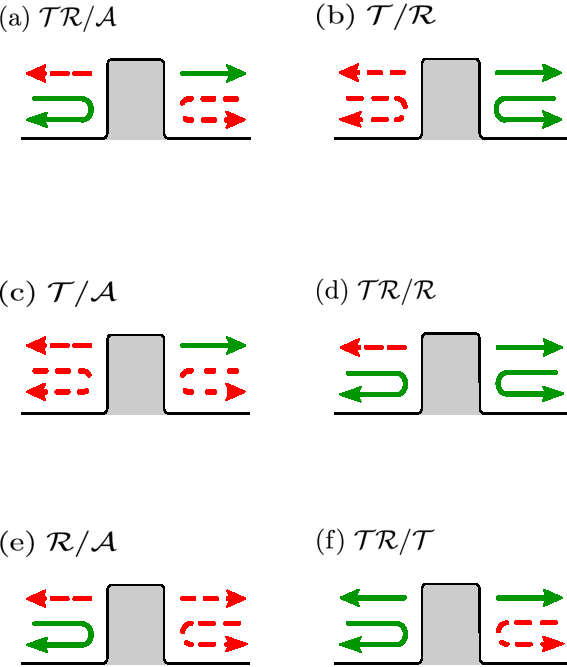
\includegraphics[width = 0.5\linewidth]{Figures/PotentialCasesPT.pdf}
  \caption{Devices with asymmetric scattering (limited to scattering coefficients being 0 or 1).  The dashed and continuous lines represent respectively zero or one
  for the moduli of the scattering amplitudes; the bended lines are for reflection amplitudes, and the straight lines for transmission:
  (a) One-way mirror ($\cal{TR/A}$); (b) One-way barrier ($\cal{T/R}$); (c) One-Way T-filter ($\cal{T/A}$);
  (d) Mirror \& 1-way transmitter ($\cal{TR/R}$); (e) One-way R-filter ($\cal{R/A}$); (f) Transparent, one-way
  reflector ($\cal{TR/T}$). The nomenclature for the devices is explained in the main text of section \ref{sec:chapter1_AsymmetricDevices}
  % The letter codes summarize the effect of left and right incidence, separated by a  slash ``$/$''.
  % ${\cal T}$ or ${\cal R}$ on one side of the slash indicate a unit
  % transmission or reflection coefficient
  % for  incidence from that side, whereas the absence of one or the other letter corresponds to zero coefficients.
  % An ${\cal A}$ denotes ``full absorption'', i.e., both moduli of reflection and transmission amplitudes are zero for incidence from one side.
  % For example,  $\cal{TR/A}$ means unit modulus transmission
  % and reflection from the left and total absorption from the right.
  \label{fig:chapter1_cases}}
\end{figure}

\section{Non-Hermitian scattering in 1 dimension \label{sec:chapter1_ScattFormalism}}

In this section I will put together the minimum set of ideas and tools needed to describe scattering in 1 dimension. The ideas in the section can be found with more detail in \cite{Muga2004}, which generalizes the results in the celebrated book by Taylor \cite{Taylor1972} to non-Hermitian Hamiltonians. In scattering theory one deals with the Hamiltonian for a particle of mass $m$ subjected to the action of a potential $V$
%
\begin{equation}
  H =  H_0 + V,
\end{equation}
%
where $H_0=\frac{P^2}{2m}$ is the kinetic energy operator, with $P$ the momentum operator. The potential $V$ is not assumed to be either hermitian or local. Before continuing, I shall clarify these two statements. A linear operator $\mathcal{O}$ is hermitian, or also self-adjoint, if it is equal to its adjoint operator $\mathcal{O}^\dagger$. The definition of the adjoint of a linear operator is given by the equation
%
\begin{equation}
  \braket{\phi}{\mathcal{O}\psi} = \braket{\mathcal{O}^\dagger\phi}{\psi}\quad\forall\ket{\psi},\,\ket{\phi}\in\mathcal{H},
  \label{eq:chapter1_adjointLinearOperators}
\end{equation}
%
Where $\mathcal{H}$ is the Hilbert space of the particle. A potential $V$ with a diagonal representation in the position basis $\{\ket{x}\}$ of the particle's Hilbert space is said to be local,
%
\begin{equation}
  \mel{x}{V_{local}}{x'} = \delta(x-x')V(x'),
  \label{eq:chapter1_localPotential}
\end{equation}
%
whereas a non local potential has off-diagonal elements
%
\begin{equation}
  \mel{x}{V_{non local}}{x'} = V(x,x').
  \label{eq:chapter1_nonLocalPotential}
\end{equation}
%
The potentials that we study are then non-diagonal and satisfy $V \neq V^\dagger$, therefore, the Hamiltonians will also be non-hermitian, $H \neq H^\dagger$.

Scattering theory addresses the following question: given an input (incident) wave packet $\ket{\psi_{in}}$, what is the output (outgoing) wave packet $\ket{\psi_{out}}$ after interacting with the potential? Another way of formulating the same question is: given an incoming state with a momentum $p$, what are the probability amplitudes of the state being reflected and transmited elastically (with the same energy)? To answer these questions the scattering theory brings in the scattering states, eigenstates of the Hamiltonian which belong to the continuum part of the spectrum, \textit{i.e.}, eigenstates of the Hamiltonian which are not bounded to a finite portion of the space and behave asymptotically as plane waves far from the range of action of the potential. The scattering states represent incoming waves with momentum $p$ and energy $E_p = \frac{p^2}{2m}>0$ that are partially reflected and transmitted by the potential. For a plane wave with momentum $p>0$ incoming from the left which is transmited to the right and reflected back, the scattering state $\ket{p^+}$ is asymptotically
%
\begin{equation}
  \braket{x}{p^+} =
  \begin{cases}
    \braket{x}{p} + R^l(p)\braket{x}{-p} \quad &\text{if}\; x \to -\infty
    \\
    T^l(p) \braket{x}{p} \quad &\text{if}\; x \to \infty
  \end{cases},
  \label{eq:chapter1_leftState}
\end{equation}
%
where $T^l(p)$ and $R^l(p)$ are the transmission and reflection amplitudes for left incidence. $\braket{x}{p} = \frac{1}{ \sqrt{2\pi\hbar} } e^{-i p x /\hbar} $ is the delta-normalized momentum eigenstate. Similarly, for a plane wave incoming from the right with momentum $-p \;(p>0)$ which is transmited to the left and reflected back, the scattering state $\ket{-p^+}$ is asymptotically
%
\begin{equation}
  \braket{x}{-p^+} =
  \begin{cases}
    T^r(p) \braket{x}{-p} \quad &\text{if}\; x \to -\infty
    \\
    \braket{x}{-p} + R^r(p)\braket{x}{p} \quad &\text{if}\; x \to \infty
  \end{cases},
  \label{eq:chapter1_rightState}
\end{equation}
%
where $T^r(p)$ and $R^r(p)$ are the transmission and reflection coefficients for right incidence. We shall see that in general $T^l\neq T^r$, $R^l\neq R^r$ for Hamiltonians that are nonhermitian and non-local. For the adjoint of the Hamiltonian $H^\dagger = \frac{P^2}{2m} + V^\dagger$, we can also find the scattering states and scattering amplitudes for left and right incidence for the adjoint: $\widehat{T}^l(p)$, $\widehat{R}^l(p)$, $\widehat{T}^r(p)$ and $\widehat{R}^r(p)$. In the rest of this Thesis I will use the convention that hatted variables $\widehat{...}$ will refer to the adjoint Hamiltonian $H^\dagger$. In the following, all the results I write down for $H$ can be obtained also for $H^\dagger$ by making the change $H \to H^\dagger$.

Scattering theory provides the method to calculate the scattering amplitudes through the transition operator $T_{op}(z)$, which is defined as
%
\begin{equation}
T_{op}(z) = V + VG(z)V,
\label{eq:chapter1_transitionOperator_definition}
\end{equation}
%
with $G(z) = (z-H)^{-1}$ being the Green's operator. In \cite{Muga2004} the transition operator is used to write the scattering eigenstates as
%
\begin{equation}
  \ket{\pm p^+} =  \ket{\pm p} + \lim_{ \varepsilon\to 0^+ } G^0(E_p + i\varepsilon)T_{op}(E_p + i\varepsilon)\ket{\pm p}\quad (p>0),
  \label{eq:chapter1_scatteringStateFormal}
\end{equation}
%
where $G^0(z) = (z-H_0)^{-1}$ is the Green's operator of the free propagation Hamiltonian $H_0$. Now, to find the scattering amplitudes of reflection and transmission, one has to take the limits of $\braket{x}{\pm p^+}$, where $\ket{\pm p^+}$ is given by eq. \eqref{eq:chapter1_scatteringStateFormal}, when $|x|$ goes to infinity and compare with eqs. \eqref{eq:chapter1_leftState}, \eqref{eq:chapter1_rightState} to get
%
\begin{align}
R^l&=-i\frac{2\pi m}{p}\la -p|T_{op}(+)|p\ra\nonumber,
\\
T^l&=1-i\frac{2\pi m}{p} \la p|T_{op}(+)|p\ra\nonumber,
\\
R^r&=-i\frac{2\pi m}{p}\la p|T_{op}(+)|-p\ra\nonumber,
\\
T^r&=1-i\frac{2\pi m}{p}\la -p|T_{op}(+)|-p\ra,
\label{eq:chapter1_amplitudesFromTOperator}
\end{align}
%
where $T_{op}(+)$ is a shorthand notation for $\lim_{ \varepsilon\to 0^+ } T_{op}(E_p + i\varepsilon)$. The same procedure can be followed using the transition operator $\widehat{T}_{op}$ for $H^\dagger$ to obtain $\widehat{T}^l(p)$, $\widehat{R}^l(p)$, $\widehat{T}^r(p)$ and $\widehat{R}^r(p)$. It is convenient to introduce the on-shell scattering matrix, defined as
%
\begin{equation}
  \mathsf{S}(p) =
  \left(
  \begin{array}{cc}
    T^l(p)&R^r(p)
    \\
    R^l(p)&T^r(p)
  \end{array}
  \right),
  \label{eq:chapter1_onShellMatrix}
\end{equation}
%
which gives the reflected and transmited components for an incident plane wave. Waves propagating from left to right are represented as $\left(1,0\right)^\mathsf{T}$ and waves propagating from right to left as $\left(0,1\right)^\mathsf{T}$. Therefore, a left incident wave will be scattered to $\left(T^l(p),R^l(p)\right)^\mathsf{T}$ and a right incident wave to $\left(R^r(p),T^r(p)\right)^\mathsf{T}$.

As I mentioned before, one of the goals of scattering theory is connecting an input state $\ket{\psi_{in}}$ with an output state $\ket{\psi_{out}}$. In scattering theory the way of doing this is through the collision or scattering operator $S$
%
\begin{equation}
  \ket{\psi_{out}} = S \ket{\psi_{in}}
  \label{eq:chapter1_actuationOfSOperator}.
\end{equation}
%
$S$ is the product of the M\"{o}ller operators $S = \Omega_{-}^\dagger\Omega_{+}$, which are defined as
%
\begin{align}
    \Omega_+ &= \lim_{t \to -\infty}e^{i H t / \hbar}e^{-i H_0 t/ \hbar},\nonumber\\
    \Omega_- &= \lim_{t \to +\infty}e^{i H^\dagger t/ \hbar}e^{-i H_0 t/ \hbar}.
    \label{eq:chapter1_MollerDefinition}
\end{align}
%
The M\"{o}ller $\widehat{\Omega}_\pm$ and scattering $\widehat{S}$ operators for the adjoint Hamiltonian can be found by substituting $H$ for $H^\dagger$ in eq. \eqref{eq:chapter1_MollerDefinition}. The M\"{o}ller operator with the +(-) symbol connects the input (output) state with the scattering states of the Hamiltonian. The M\"{o}ller operators satisfy the isometry relation
%
\begin{equation}
  \Omega_\pm^\dagger \Omega_\pm = 1,
  \label{eq:chapter1_MollerIsometry}
\end{equation}
%
and the following intertwining equations with the complete and free Hamiltonians $H$, $H_0$
%
\begin{align}
  H\Omega_+ &= \Omega_+ H_0,\nonumber
  \\
  H^\dagger\Omega_- &= \Omega_- H_0.
  \label{eq:chapter1_MollerIntertwining}
\end{align}
%
The hatted quantities for the adjoint Hamiltonian have expressions similar to those in eqs. \eqref{eq:chapter1_MollerIsometry} and \eqref{eq:chapter1_MollerIntertwining} with the substitution $H\leftrightarrow H^\dagger$. Because of eq. \eqref{eq:chapter1_MollerIntertwining} and because the momentum eigenstates $\ket{p}$ are eigenstates of $H_0$ with energy $E_p$ we have that the scattering states in eqs. \eqref{eq:chapter1_leftState}, \eqref{eq:chapter1_rightState} are also given by
%
\begin{equation}
  \ket{\pm p^+} = \Omega_+ \ket{\pm p}\quad (p>0).
  \label{eq:chapter1_scatteringStateFromMoller}
\end{equation}
%
%
It is immediate to see, that since the Hamiltonian may not be hermitian, the scattering operator will not be unitary in general. Because of this non-unitarity, input states may, for example, be absorbed by the potential. However, the scattering operator $S$ and the scattering operator $\widehat{S}$ of the adjoint Hamiltonian $H^\dagger$ satisfy the generalized unitarity relation
%
\begin{equation}
  \widehat{S}^\dagger S = S\widehat{S}^\dagger= 1.
  \label{eq:chapter1_SMatrixUnitarityGeneralized}
\end{equation}
%
The generalized unitary relation \eqref{eq:chapter1_SMatrixUnitarityGeneralized} implies a set of relations for the scattering amplitudes of non-Hermitian Hamiltonians. To find these relations one needs to find the matrix elements of $S$, $\widehat{S}$ in the momentum basis. According to \cite{Muga2004} the matrix elements of the scattering operator are related to the transition operator by
%
\begin{equation}
    \bra{p} S \ket{p'} = \delta (p-p') -2 i \pi \delta (E_p-E_{p'}) \bra{p}T_{op}(+)\ket{p'},
    \label{eq:SmatrixElements}
\end{equation}
%
If we factor the dirac delta in momentum using that $\delta(p-p') = \frac{|p|}{m}\delta(E_{p}-E_{p'})$ and consider positive momenta $p$ and $p'$ we get
%
\begin{equation}
  \left(
  \begin{array}{cc}
    \mel{p}{S}{p'} & \mel{p}{S}{-p'}\\
    \mel{-p}{S}{p'} & \mel{-p}{S}{-p'}
  \end{array}
  \right)
  = \frac{|p|}{m}\delta(E_{p}-E_{p'})\mathsf{S}(p).
  \label{eq:chapter1_onShellMatrixRelationToS}
\end{equation}
%
Because of \eqref{eq:chapter1_onShellMatrixRelationToS}, the on-shell scattering matrices $\mathsf{S}$ and $\mathsf{\widehat{S}}$ (of the adjoint Hamiltonian) inherit the generalized unitarity relation of the scattering operators \eqref{eq:chapter1_SMatrixUnitarityGeneralized}, yielding the following useful relations for the scattering amplitudes
%
\begin{equation}
  \mathsf{\widehat{S}}^\dagger\mathsf{S} = \mathsf{1}
  \Longrightarrow
  \begin{cases}
    %
    \widehat T^l(p) T^{l*}(p) + \widehat R^l(p) R^{l*}(p) &= 1,
    %
    \\
    %
    \widehat T^r(p) T^{r*}(p) + \widehat R^r(p) R^{r*}(p) &= 1,
    %
    \\
    %
    \widehat T^{l*}(p) R^r(p) + T^r(p) \widehat R^{l*}(p) &= 0,
    %
    \\
    %
    T^l(p) \widehat R^{r*}(p) + \widehat T^{r*}(p) R^l(p) &= 0,
    %
  \end{cases}
  \label{eq:chapter1_unitarityCoefficients}
\end{equation}
%
The relations in \eqref{eq:chapter1_unitarityCoefficients} will be extremely relevant for the rest of the Thesis, as they set extra conditions for the scattering amplitudes of asymmetry devices.

\subsection{Why is non-Hermiticity needed for asymmetric scattering?}

Asymmetric scattering is achieved when $\left|T^l\right|\neq\left|T^r\right|$ and $\left|R^l\right|\neq\left|R^r\right|$. When the Hamiltonian is hermitian, the hatted ($\widehat{\cdot}$) quantities in eq. \eqref{eq:chapter1_unitarityCoefficients} are equal to the unhatted ones and therefore eq. \eqref{eq:chapter1_unitarityCoefficients} becomes
%
\begin{align}
  \left|T^l(p)\right|^2 +  \left|R^l(p)\right|^2  &= 1,\nonumber
  %
  \\
  %
  \left|T^r(p)\right|^2 +  \left|R^r(p)\right|^2  &= 1,\nonumber
  %
  \\
  %
   T^{l*}(p) R^r(p) + T^r(p)  R^{l*}(p) &= 0.
  %
  \label{eq:chapter1_unitarityCoefficients_HermitianCase}
\end{align}
%
Taking absolute values in the last equation in \eqref{eq:chapter1_unitarityCoefficients_HermitianCase} and solving for $T^{r}(p)$ gives
%
\begin{equation}
  \left|T^r(p)\right|  = \left| T^{l}(p) \frac{R^r(p)}{R^{l}(p)} \right|.
\end{equation}
%
Now, because of the first equation in \eqref{eq:chapter1_unitarityCoefficients_HermitianCase} we get $\left|R^r(p)\right| = \left|R^l(p)\right|$. Finally, substracting the two first equations in \eqref{eq:chapter1_unitarityCoefficients_HermitianCase} one arrives at $\left|T^r(p)\right| = \left|T^l(p)\right|$. Therefore, it is impossible to build asymmetric devices with hermitian Hamiltonians.

\section{Right and left eigenvectors of non-hermitian Hamiltonians\label{sec:chapter1_LeftAndRightEigenstates}}

Eigenstates in the discrete part of the spectrum (bound-in-space eigenstates) of a hermitian Hamiltonian corresponding to different eigenvalues are orthogonal, \textit{i.e.} $\braket{E_i}{E_j} =0$ if $E_i\neq E_j$. Assuming there are no degenerate eigenvalues (for simplicity) one can choose the normalization $\braket{E_i}{E_j} =\delta_{ij}$, which makes the  eigenstates an orthonormal set. Similarly, the scattering states $\ket{p^+}$ satisfy (in the hermitian case) $\braket{p^+}{p'^+} =\delta(p-p')$. The discrete and scattering eigenstates are orthonormal bases in their corresponding subspaces and can be used to form a basis of the complete Hilbert space in the following way
%
\begin{equation}
  1 = \sum_i \ketbra{E_i}{E_i} + \int dp\; \ketbra{p^+}{p^+}
  \label{eq:chapter1_HermitianHamiltonianBasis}
\end{equation}
%
However, if the Hamiltonian is non-Hermitian, the completeness formula \eqref{eq:chapter1_HermitianHamiltonianBasis} will not be correct anymore. It is possible, however, to generalize \eqref{eq:chapter1_HermitianHamiltonianBasis} to the hermitian case with the concept of left eigenvectors and bi-orthogonal partners. We say that the vectors $\ket{\lambda}$ and $\ket{\widehat{\lambda}}$ are a right and a left pair of eigenvectors if there exists a $\lambda$ eigenvalue such that
%
\begin{align}
  H \ket{\lambda} &= \lambda \ket{\lambda},\nonumber\\
  \bra{\widehat{\lambda}} H  &= \bra{\widehat{\lambda}}\lambda.
  \label{eq:chapter1_leftAndRightEigenvector}
\end{align}
%
If one takes two different eigenvalues $\lambda_1$ and $\lambda_2$, it is easy to show that $\braket{\widehat{\lambda_1}}{\lambda_2}=\braket{\widehat{\lambda_2}}{\lambda_1}=0$, and for this reason, the pairs $\ket{\lambda},\,\ket{\widehat{\lambda}}$ are called biorthogonal partners. This result is applied to scattering Hamiltonians in the following way. If we assume, for simplicity, that there is no degeneracy in the discrete spectrum of $H$, we can choose the normalization $\braket{\widehat{E_i}}{E_j} = \delta_{ij}$ for the point spectrum eigenvectors. The right scattering states are given by eq. \eqref{eq:chapter1_scatteringStateFromMoller}. Using the intertwining relations \eqref{eq:chapter1_MollerIntertwining} for the hatted Moller operators (after the $H\leftrightarrow H^\dagger$ substitution) one can prove that the states $\ket{\widehat{p}^+} = \widehat{\Omega}_+\ket{p}$ are left eigenvectors of $H$ with eigenvalue $E_p$. The isometry relation \eqref{eq:chapter1_MollerIsometry} implies $\braket{\widehat{p}^+}{q^+} = \delta(q-p)$, therefore the pairs $\ket{\widehat{p}^+}$, $\ket{p^+}$ are biorthogonal partners. Finally, the completeness formula of the Hilbert space \eqref{eq:chapter1_HermitianHamiltonianBasis} is generalized to the non-Hermitian case as
%
\begin{equation}
  1 = \sum_i \ketbra{E_i}{\widehat{E}_i} + \int dp\; \ketbra{p^+}{\widehat{p}^+}.
  \label{eq:chapter1_NonHermitianHamiltonianBasis}
\end{equation}
%

\section{Generalized symmetries\label{sec:chapter1_generalizedSymmetries}}

For hermitian  Hamiltonians, symmetries are represented by the commutation of some symmetry operator $A$ with the Hamiltonian. According to Wigner's theorem \cite{Wigner1959}, a symmetry operator $A$ has to be either unitary or antiunitary. Unitary and antiunitary operators are defined by the relation $A^\dagger A = A A^\dagger = 1$. Unitary operators are linear, and therefore the adjoint is defined by eq. \eqref{eq:chapter1_adjointLinearOperators}, whereas antiunitary operators are antilinear, so the adjoint is defined by
%
\begin{equation}
  \braket{\phi}{\mathcal{O}\psi} = \braket{\mathcal{O}^\dagger\phi}{\psi}^*\quad\forall\ket{\psi},\,\ket{\phi}\in\mathcal{H}.
  \label{eq:chapter1_adjointAntiLinearOperators}
\end{equation}
%
In scattering theory, symmetry plays an important role  as it implies relations among
the S-matrix elements beyond those implied by its unitarity, see e.g. \cite{Taylor1972} and, for scattering in one dimension, Sec. 2.6 in \cite{Muga2004}. Symmetries are also useful for  non-Hermitian Hamiltonians, but the mathematical and conceptual
framework must be generalized. We consider that a unitary or antiunitary operator $A$ represents a symmetry of $H$ if it satisfies at least one of these relations,
%
\begin{eqnarray}
  AH&=&HA,
  \label{eq:chapter1_symmetry}
  \\
  AH&=&H^\dagger A,
  \label{eq:chapter1_pseudoSymmetry}
\end{eqnarray}
%
For a right eigenstate of $H$, $|\psi\rangle$,
with eigenvalue $E$, eq. (\ref{eq:chapter1_symmetry}) implies that
$A|\psi\rangle$ is also a right  eigenstate of $H$, with the
same eigenvalue if $A$ is unitary, and with the complex conjugate eigenvalue $E^*$ if $A$ is antiunitary.
Equation (\ref{eq:chapter1_pseudoSymmetry}) implies that $A|\psi\rangle$ is a right eigenstate of $H^\dagger$
with eigenvalue $E$ for $A$ unitary or $E^*$ for $A$ antiunitary, or a left eigenstate of $H$ with eigenvalue $E^*$ for $A$ unitary, or $E$
for $A$ antiunitary. For real-energy scattering
eigenfunctions in the continuum, the ones we are interested in here, $E^*=E$.
When eq. (\ref{eq:chapter1_pseudoSymmetry}) holds we say that $H$ is $A$-pseudohermitian \cite{Mostafazadeh2010}.
Parity-pseudohermiticity has played an important role as being equivalent to space-time reflection (PT) symmetry for {\it local} potentials
\cite{Mostafazadeh2010,Znojil2015}. A large set of these equivalences
will be discussed below.
A relation of the form (\ref{eq:chapter1_pseudoSymmetry}) has been also used with differential operators  to get real spectra beyond
PT-symmetry for local potentials  \cite{Nixon2016,Nixon2016a}.

Here we consider
%that $H$ may be non-local, and
$A$ to be a member of the
Klein 4-group $K_4=\{1,\Pi, \Theta, \Pi\Theta\}$ formed by unity, the parity operator $\Pi$, the antiunitary time-reversal operator $\Theta$, and their product
$\Pi\Theta$. The Klein 4-group is a discrete, Abelian group and every element $A$ satisfies $A^2 = 1$. We also assume that the  Hamiltonian is  of the form $H=H_0+V$, with $H_0$, the kinetic energy operator of the particle,
being hermitian and
satisfying $[H_0,A]=0$ for all members of the group, whereas the potential $V$ may be non-local in position representation.
The  motivation to use Klein's group is that the eight relations implied by eqs. (\ref{eq:chapter1_symmetry}) and (\ref{eq:chapter1_pseudoSymmetry}) generate all
possible symmetry transformations of a non-local potential due to the identity, complex conjugation, transposition, and sign inversion,
both in coordinate or momentum representation, see 3rd and 4th columns of table \ref{tab:chapter1_SymmetriesTable}, where each symmetry has been labeled by a roman number.

% ----------------------------------------------------------------------------------------------
\begin{landscape}
  \begin{table}
    \caption{Symmetries of the potential classified in terms of the commutativity or pseudo-Hermiticity of $H$ with the elements of
    Klein's 4-group  $\{1,\Pi,\theta,\Pi\theta\}$ (second column). The first column sets a simplifying roman-number code for each symmetry.
    The relations among potential matrix elements are given in coordinate and momentum representations in the third and fourth columns.
    The fifth column gives the relations they imply in the matrix elements of $S$ and/or $\widehat{S}$ matrices ($S$ is for scattering by $H$
    and $\widehat{S}$ for scattering by $H^\dagger$). From them  the next four columns set the relations implied on scattering amplitudes.
    Together with generalized unitarity relations (\eqref{eq:chapter1_unitarityCoefficients}) they also imply relations for the moduli (tenth column), and phases (not shown). The last two columns indicate the possibility to achieve perfect asymmetric transmission or reflection:  ``${P}$" means possible (but not necessary),
    ``No'' means impossible.  In some cases ``$P$" is accompanied by a condition that must be satisfied.\vspace*{.2cm}
    \label{tab:chapter1_SymmetriesTable}}
    \centering
    \scalebox{.8}{
    \begin{tabular}{cccccccccccc}
      \hline\hline\\
      (1)&(2)&(3)&(4)&(5)&(6)&(7)&(8)&(9)&(10)&(11)&(12)\\
      Code & Symmetry&  $\langle x|V|y\rangle=$ & $\langle p|V|p'\rangle=$ & $\langle p|S|p'\rangle=$ & $T^l\!=$ & $T^r\!=$ & $R^l\!=$& $R^r\!=$& from eq. (\eqref{eq:chapter1_unitarityCoefficients})&$|T^l|\!=\!1$&$|R^l|\!=\!1$
      \\
      &&&&&&&&&&$|T^r|\!=\!0$&$|R^r|\!=\!0$
      \\
      \hline
      I & $1H=H1$ &   $\langle x|V|y\rangle$ & $\langle p|V|p'\rangle$ & $\langle p|S|p'\rangle$ & $T^l$ & $T^r$ & $R^l$ & $R^r$ & & $P$ & $P$
      \\
      II & $1H=H^\dagger 1$ &  $\langle y|V|x\rangle^*$ & $\langle p'|V|p\rangle^*$ &$\langle p|\widehat{S}|p'\rangle$ & $\widehat{T}^l$& $\widehat{T}^r$ & $\widehat{R}^l$ & $\widehat{R}^r$
      & $|T^l|\!=\!|T^r|$, $|R^l|\!=\!|R^r|$&No&No
      \\
      III & $\Pi H=H\Pi$ &  $\langle -x|V|-y\rangle$ & $\langle -p|V|-p'\rangle$ &$\langle -p|S|-p'\rangle$ & $T^r$ & $T^l$ & $R^r$ & $R^l$& $|T^l|\!=\!|T^r|$,$ |R^l|\!=\!|R^r|$ &No&No
      \\
      IV & $\Pi H=H^\dagger \Pi$ &  $\langle -y|V|-x\rangle^*$ & $\langle -p'|V|-p\rangle^*$ & $\langle -p|\widehat{S}|-p'\rangle$ & $\widehat{T}^r$ & $\widehat{T}^l$ & $\widehat{R}^r$ & $\widehat{R}^l$&&$P$, $R^rR^{l*}=1$&$P$, $T^r{T^l}^*=1$
      \\
      V & $\Theta H=H\Theta$ &  $\langle x|V|y\rangle^*$& $\langle -p|V|-p'\rangle^*$ & $\langle -p'|\widehat{S}|-p\rangle$ & $\widehat{T}^r$ & $\widehat{T}^l$ & $\widehat{R}^l$& $\widehat{R}^r$
      &$|R^l|=|R^r|$&$P$, $|R^{r,l}|=1$&No
      \\
      VI & $\Theta H=H^\dagger\Theta$ &  $\langle y|V|x\rangle$& $\langle -p'|V|-p\rangle$ & $\langle -p'|S|-p\rangle$ & $T^r$& $T^l$ & $R^l$& $R^r$&$|T^l| = |T^r|$&No&$P$
      \\
      VII & $\Theta\Pi H=H\Theta \Pi$ &  $\langle -x|V|-y\rangle^*$ & $\langle p|V|p'\rangle^*$ & $\langle p'|\widehat{S}|p\rangle$ &$\widehat{T}^l$& $\widehat{T}^r$ & $\widehat{R}^r$& $\widehat{R}^l$&$|T^l|=|T^r|$&No&$P$, $|T^{r,l}|=1$
      \\
      VIII& $\Theta\Pi H=H^\dagger \Theta \Pi$ &  $\langle -y|V|-x\rangle$ & $\langle p'|V|p\rangle$ & $\langle p'|S|p\rangle$ & $T^l$ & $T^r$ & $R^r$ & $R^l$&$|R^l|=|R^r|$&$P$&No
      \\
      \hline\hline
    \end{tabular}}
  \end{table}
\end{landscape}
% ----------------------------------------------------------------------------------------------


\begin{table}
  \caption{Transformation rules of the M\"oller and scattering operators under symmetries/pseudo-symmetries with linear or antilinear operators.}
  \label{tab:chapter1_MollerOperatorSymmetries}
  \centering
  \begin{tabular}{lcc}
  \hline\hline\\
  \textbf{Type of symmetry} & \textbf{$A$ linear} & \textbf{$A$ antilinear}

  \\
  \hline
  $A H = H A$
  &
  $
  \begin{array}{ccc}
    &&
    \\
    A \Omega_{\pm}&=&\Omega_{\pm} A
    \\
    A S&=&S A
    \\
    &&
  \end{array}
  $
  &
  $
  \begin{array}{ccc}
    &&
    \\
    A \Omega_{\pm}&=&\widehat{\Omega}_{\mp} A
    \\
    A S&=&\widehat{S}^\dagger A
    \\
    &&
  \end{array}
  $
  \\
  $A H = H^\dagger A$
  &
  $
  \begin{array}{ccc}
    &&
    \\
    A \Omega_{\pm}&=&\widehat{\Omega}_{\pm} A
    \\
    A S&=&\widehat{S} A
    \\
    &&
  \end{array}
  $
  &
  $
  \begin{array}{ccc}
    &&
    \\
    A \Omega_{\pm}&=&\Omega_{\mp} A
    \\
    A S&=&S^\dagger A
    \\
    &&
  \end{array}
  $
  \\
  \hline\hline
  \end{tabular}
\end{table}

With the definitions of symmetry in eqs. \eqref{eq:chapter1_symmetry}, \eqref{eq:chapter1_pseudoSymmetry} and the tools from scattering formalism in \ref{sec:chapter1_ScattFormalism} we can now derive the effects of the symmetries in the scattering operator $S$, which will pose restrictions in the scattering amplitudes. We start by deriving the transformation rules of the M\"{o}ller operators \eqref{eq:chapter1_MollerDefinition} under a symmetry operator $A$ of the Klein 4-group. The M\"{o}ller operators are transformed differently depending on whether $A$ is unitary or antiunitary and whether the Hamiltonian obeys usual symmetry \eqref{eq:chapter1_symmetry} or pseudohermiticity \eqref{eq:chapter1_pseudoSymmetry}. For example, for $A$ unitary and \eqref{eq:chapter1_symmetry} we have
%
\begin{equation}
  \begin{split}
    A \Omega_+ &= A \lim_{t \to -\infty} e^{i H t/\hbar}e^{-i H_0 t/\hbar}\\
    &= \lim_{t \to -\infty}e^{i H t/\hbar}Ae^{-i H_0 t/\hbar}\\
    &= \lim_{t \to -\infty} e^{i H t/\hbar}e^{-i H_0 t/\hbar}A\\
    &= \Omega_+ A,
  \end{split}
  \label{eq:chapter1_MollerPositiveTransformAUnitary_Symmetry}
\end{equation}
%
and
%
\begin{equation}
  \begin{split}
    A \Omega_- &= A \lim_{t \to +\infty} e^{i H^\dagger t/\hbar}e^{-i H_0 t/\hbar}\\
    &= \lim_{t \to +\infty}e^{i H^\dagger t/\hbar}Ae^{-i H_0 t/\hbar}\\
    &= \lim_{t \to +\infty} e^{i H^\dagger t/\hbar}e^{-i H_0 t/\hbar}A\\
    &= \Omega_- A.
  \end{split}
  \label{eq:chapter1_MollerNegativeTransformAUnitary_Symmetry}
\end{equation}
%
Using eqs. \eqref{eq:chapter1_MollerPositiveTransformAUnitary_Symmetry} and \eqref{eq:chapter1_MollerNegativeTransformAUnitary_Symmetry} we finally get
%
\begin{equation}
  \begin{split}
    A S &= A \Omega_{-}^\dagger\Omega_{+} \\
    &= \Omega_{-}^\dagger A \Omega_{+} \\
    &= \Omega_{-}^\dagger\Omega_{+} A \\
    &= S A,\\
    &\Downarrow\\
    S &= A^{\dagger}SA.
  \end{split}
  \label{eq:chapter1_Moller-TransformAUnitary_Symmetry}
\end{equation}
%
The rest of combinations of the type of $A$ (unitary/antiunitary) with the type of symmetry (\eqref{eq:chapter1_symmetry} or \eqref{eq:chapter1_pseudoSymmetry}) are summarized in table \ref{tab:chapter1_MollerOperatorSymmetries}. Since the symmetry operators conmute with the free Hamiltonian $H_0$, the action of any of them on a momentum eigenstate will give as a result a state with the same energy. In fact, as can be seen in table \ref{tab:chapter1_KleinGroupOnPosAndMomentBases} the result of the action of any element $A$ of the 4-group on a state $\ket{p}$ is either $\ket{p}$ or $\ket{-p}$. For this reason, we can work with the on-shell representation of the scattering operator to obtain extra relations between the scattering amplitudes. As an example I will demonstrate what happens to the scattering amplitudes when the symmetry III is satisified, \textit{i.e.}, $\Pi H = H \Pi$. Considering a momentum $p>0$ and using $S = \Pi^{\dagger}S \Pi$ (see table \ref{tab:chapter1_MollerOperatorSymmetries}) I find
%
\begin{equation}
  \left(
  \begin{array}{cc}
    \mel{p}{S}{p} & \mel{p}{S}{-p}\\
    \mel{-p}{S}{p} & \mel{-p}{S}{-p}
  \end{array}
  \right)
  =
  \left(
  \begin{array}{cc}
    \mel{-p}{S}{-p} & \mel{-p}{S}{p}\\
    \mel{p}{S}{-p} & \mel{p}{S}{p}
  \end{array}
  \right).
\end{equation}
%
Now, using the on-shell representation of the scattering operator \eqref{eq:chapter1_onShellMatrixRelationToS} and the definition of $\mathsf{S}(p)$ \eqref{eq:chapter1_onShellMatrix} I arrive at
%
\begin{align}
  T^l(p) &= T^r(p),\nonumber\\
  R^l(p) &= R^r(p).
  \label{eq:chapter1_effectOfPArityOnamplitudes}
\end{align}
%
Instead of deriving the equivalent relation to \eqref{eq:chapter1_effectOfPArityOnamplitudes} for all the symmetries explicitely, I summarize the results for the matrix elements of the $S$ operator in the 5th column and for the scattering amplitudes in the columns 6-9 of table \ref{tab:chapter1_SymmetriesTable}. Explicit examples on how to find the relations in the 5th and 6th columns of table \ref{tab:chapter1_SymmetriesTable} for other symmetries can be found in \cite{Muga2004}.

If we now take into account the generalized unitary relations $\widehat{S}^\dagger S=S\widehat{S}^\dagger=1$, in terms of amplitudes \eqref{eq:chapter1_unitarityCoefficients}, the columns 6-9 of table \ref{tab:chapter1_SymmetriesTable} imply further consequences on the amplitudes' moduli (tenth column of table \ref{tab:chapter1_SymmetriesTable}) and phases (not shown). The final two columns use the previous results to determine if perfect asymmetry is possible for transmission or reflection.
This makes evident that Hermiticity (II) and parity (III) preclude, independently, any asymmetry in the scattering coefficients;
PT-symmetry (VII) or  $\Theta$-pseudohermiticity
(VI) forbid transmission asymmetry (all local potentials  satisfy automatically
symmetry VI),  whereas time-reversal symmetry (i.e., a real potential in coordinate space)
(V) or  PT-pseudohermiticity (VIII) forbid reflection asymmetry.


\begin{table}
  \caption{Action of the Klein 4-group on the position and momentum bases. Each cell corresponds to the action of the elements of the Klein 4-group (in the first column) on the position and momentum eigenstates (in the first row). A scalar $\alpha \in \mathbb{C}$ is included in the table to make the unitary/antiunitary nature of the elements of the group explicit.}
  \label{tab:chapter1_KleinGroupOnPosAndMomentBases}
  \center
  \begin{tabular}{lcc}
    \hline\hline
    & $\alpha \ket{x}$ & $\alpha \ket{p}$\\
    \hline
    $1$ & $\alpha \ket{x}$ & $\alpha \ket{p}$\\ %Identity
    $\Pi$  & $\alpha \ket{-x}$ & $\alpha \ket{-p}$\\ %Parity
    $\Theta$ & $\alpha^* \ket{x}$ & $\alpha^* \ket{-p}$\\ %Time Reversal
    $\Pi\Theta$ & $\alpha^* \ket{-x}$ & $\alpha^* \ket{p}$\\ %PT
    \hline\hline
  \end{tabular}
\end{table}




\subsection{Equivalences between symmetries}

The occurrence of one particular symmetry in the potential (conventionally  ``first symmetry'')
does not exclude a second symmetry to be satisfied as well.
When a double symmetry holds, excluding the identity,  the ``first'' symmetry  implies the equivalence of the second symmetry with a third symmetry.
We have already mentioned that $\Pi$-pseudohermiticity (IV) is equivalent to $PT$-symmetry (VII) for local potentials.
Being local is just one particular way to satisfy symmetry VI, namely $\Theta$-pseudohermiticity. The reader may verify with the aid of
the third column for $\langle x|V|y\rangle$  in table \ref{tab:chapter1_SymmetriesTable}, that indeed, if symmetry VI is satisfied (first symmetry), symmetry IV has the same effect as symmetry VII.
They become equivalent. Other well known example is  that for a local potential (symmetry VI is satisfied), a real potential in coordinate space  is necessarily hermitian,
so symmetries V and II become equivalent.
These examples are just particular cases of the full set of equivalences given in table \ref{tab:chapter1_equivalencesBetweenSymmetries}.

\begin{table}
  \caption{Equivalences among symmetries for the potential elements.
  Given the symmetry of the upper row, the table provides the equivalent symmetries.
  For example, if II is satisfied, then III=IV holds. In words, if the potential is hermitian,  parity symmetry amounts to
  parity pseudohermiticity. In terms of the matrix elements of the potential, if  $\langle x|V|y\rangle=\langle y|V|x\rangle^*$ and also
  $\langle x|V|y\rangle=\langle -x|V|-y\rangle$, $\forall (x,y)$, then $\langle x|V|y\rangle=\langle -y|V|-x\rangle^*$ holds as well. One may proceed similarly for all other relations.
  The commutation with the identity (I) is excluded as this symmetry is satisfied by all potentials.\vspace*{.2cm}
  \label{tab:chapter1_equivalencesBetweenSymmetries}}
  \centering
  \scalebox{1}{
  \begin{tabular}{ccccccc}
    \hline\hline
    II & III& IV& V& VI & VII &VIII
    \\
    \hline
    III=IV & II=IV & II=III & II=VI &II=V&II=VIII&II=VII
    \\
    V=VI&V=VII&V=VIII&III=VII&III=VIII&III=V&III=VI
    \\
    VII=VIII&VI=VIII&VI=VII&IV=VIII&IV=VII&IV=VI&IV=V
    \\
    \hline\hline
  \end{tabular}}

\end{table}



\section{Asymmetric devices\label{sec:chapter1_AsymmetricDevices}}

% We propose six different types of asymmetric devices, see fig. \ref{fig:chapter1_cases}. The six types of devices are classified according to the transmission and reflection coefficients of the scattering potentials, which in the ideal case would take only values of 0 or 1. For example, the device in fig. \ref{fig:chapter1_cases}(a), called \textit{One-way mirror} ($\cal{TR/A}$) reflects back and transmits incoming wave packets with the same intensity for left incidence, whereas all the wave packets coming from the right are completely absorbed. In fig. \ref{fig:chapter1_cases}(c) the \textit{One-Way T-filter} ($\cal{T/A}$) would be the equivalent to a diode, since it transmits all the wave packet for left incidence while it behaves as an insulator for right incidence.



Now, I will describe the set of devices that we want to design and how the symmetries of the Klein 4-group make this possible or impossible in some cases. Table \ref{tab:chapter1_DevicesDescription} shows a descriptive list of the 6 kinds of asymmetric devices that we consider (see also fig. \ref{fig:chapter1_cases} for a schematic representation of the devices). The first column gives the name that we have chosen for each of the devices. Second and third columns show the expected behaviour for left or right incidence, respectively. The fourth column shows the descriptive code for each of the devices. The descriptive codes have always the following structure, \textit{LI/RI}, where LI and RI are codes that describe the behaviour for left and right incidence respectively. LI and RI can be composed by the following symbols $\mathcal{T}$, $\mathcal{R}$, $\mathcal{A}$. $\mathcal{T}$ stands for devices with full transmision ($T=1$), $\mathcal{R}$ for full reflection ($R = 1$). $\mathcal{A}$ is the code for full absortion ($R=T=0$). For example, a device with reflection asymmetry $R^l=1$, $R^r=0$ and with $T^r=T^l=1$ would in our case be a particular ``transparent, one-way reflector'', as full transmission occurs from both sides and its descriptive code would be $\mathcal{T}\mathcal{R}/\mathcal{T}$. This effect has however become popularized as ``unidirectional invisibility'' \cite{Lin2011,Yin2013}. The device denominations in fig. \ref{fig:chapter1_cases} or table \ref{tab:chapter1_DevicesDescription} are intended as short and meaningful, and do not necessarily coincide with some extended terminology, in part because the range of possibilities is broader here than those customarily considered, and because we use a 1 or 0 condition for the moduli.

Combining the information of the last two-columns in table \ref{tab:chapter1_SymmetriesTable} with the additional condition that all scattering coefficients
be 0 or 1 we elaborate the last two columns of table \ref{tab:chapter1_DevicesDescription}, which provides the symmetries
that do not allow the implementation of the devices in fig. \ref{fig:chapter1_cases}. The complementary table \ref{tab:chapter1_AllowedDevices} gives instead the symmetries that allow, but do not necessarily imply, a given device type.




\begin{landscape}
  \begin{table}
    \caption{Device types for  transmission and/or reflection asymmetry, restricted to 1 or 0 moduli for the scattering amplitudes.¡''
    % (i.e., zero scattering amplitudes for transmission and reflection from the right).
    The fifth column indicates the symmetries in table \ref{tab:chapter1_SymmetriesTable} that forbid the device. Figures S2, S3, S5 and S6 can be found in the supplemental material to this paper.\vspace*{.2cm}}
    \label{tab:chapter1_DevicesDescription}
    \centering
    \scalebox{1}{
    \begin{tabular}{ccccccc}
      \hline\hline
      Device type & Left incidence& Right incidence&Code& Forbidden by & Example
      \\
      \hline
      One-way mirror&transmits and reflects&absorbs&$\cal{TR/A}$&II, III, IV, V, VI,  VII, VIII&
      \\
      One-way barrier&transmits&reflects&$\cal{T/R}$&II, III, IV, V, VI, VII, VIII&
      \\
      One-way T-filter&transmits&absorbs&$\cal{T/A}$&II, III, IV, V, VI, VII&fig. \ref{fig_device_T_A}
      \\
      Mirror\&1-way transmitter&transmits and reflects&reflects&$\cal{TR/R}$&II, III, VI, VII
      \\
      One-way R-filter&reflects&absorbs&$\cal{R/A}$&II, III, IV, V, VII, VIII&\cite{Huang2016}
      \\
      Transparent 1-way reflector&transmits and reflects&transmits&$\cal{TR/T}$& II, III, V, VIII
      & figs. \ref{fig_reflector}
      \\
      \hline\hline
    \end{tabular}}
  \end{table}
\end{landscape}


\begin{table}
  \caption{Device types allowed for a given symmetry.
  \vspace*{.3cm}\label{tab:chapter1_AllowedDevices}}
  \centering
  \scalebox{0.9}{
  \begin{tabular}{cc}
    \hline\hline
    Symmetry& Allowed devices
    \\
    \hline
    I&All types
    \\
    II&None
    \\
    III&None
    \\
    IV&$\cal{TR/R,TR/T}$
    \\
    V&$\cal{TR/R}$
    \\
    VI & $\cal{R/A, TR/T}$
    \\
    VII&$\cal{TR/T}$
    \\
    VIII&$\cal{T/A,TR/R}$
    \\
    \hline\hline
  \end{tabular}}

\end{table}


%%%%%%%%%

\begin{figure}
  \begin{center}
    (a)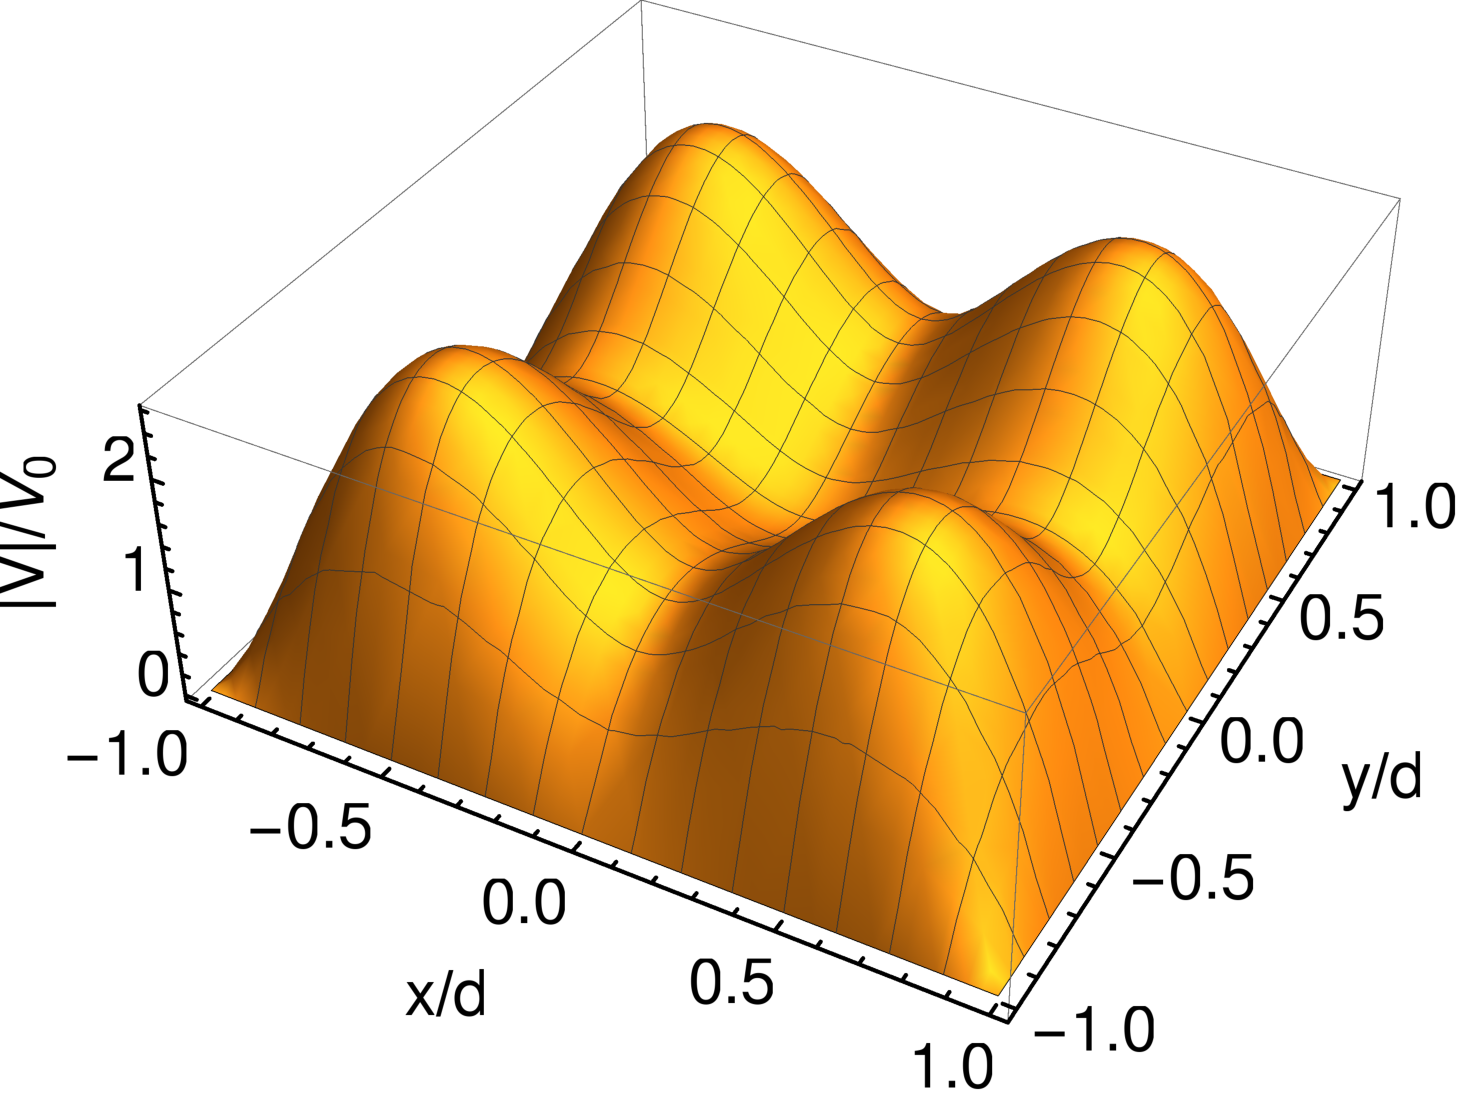
\includegraphics[width = 0.6\columnwidth]{Figures/fig_T_A_pot_abs.pdf}\\
    (b)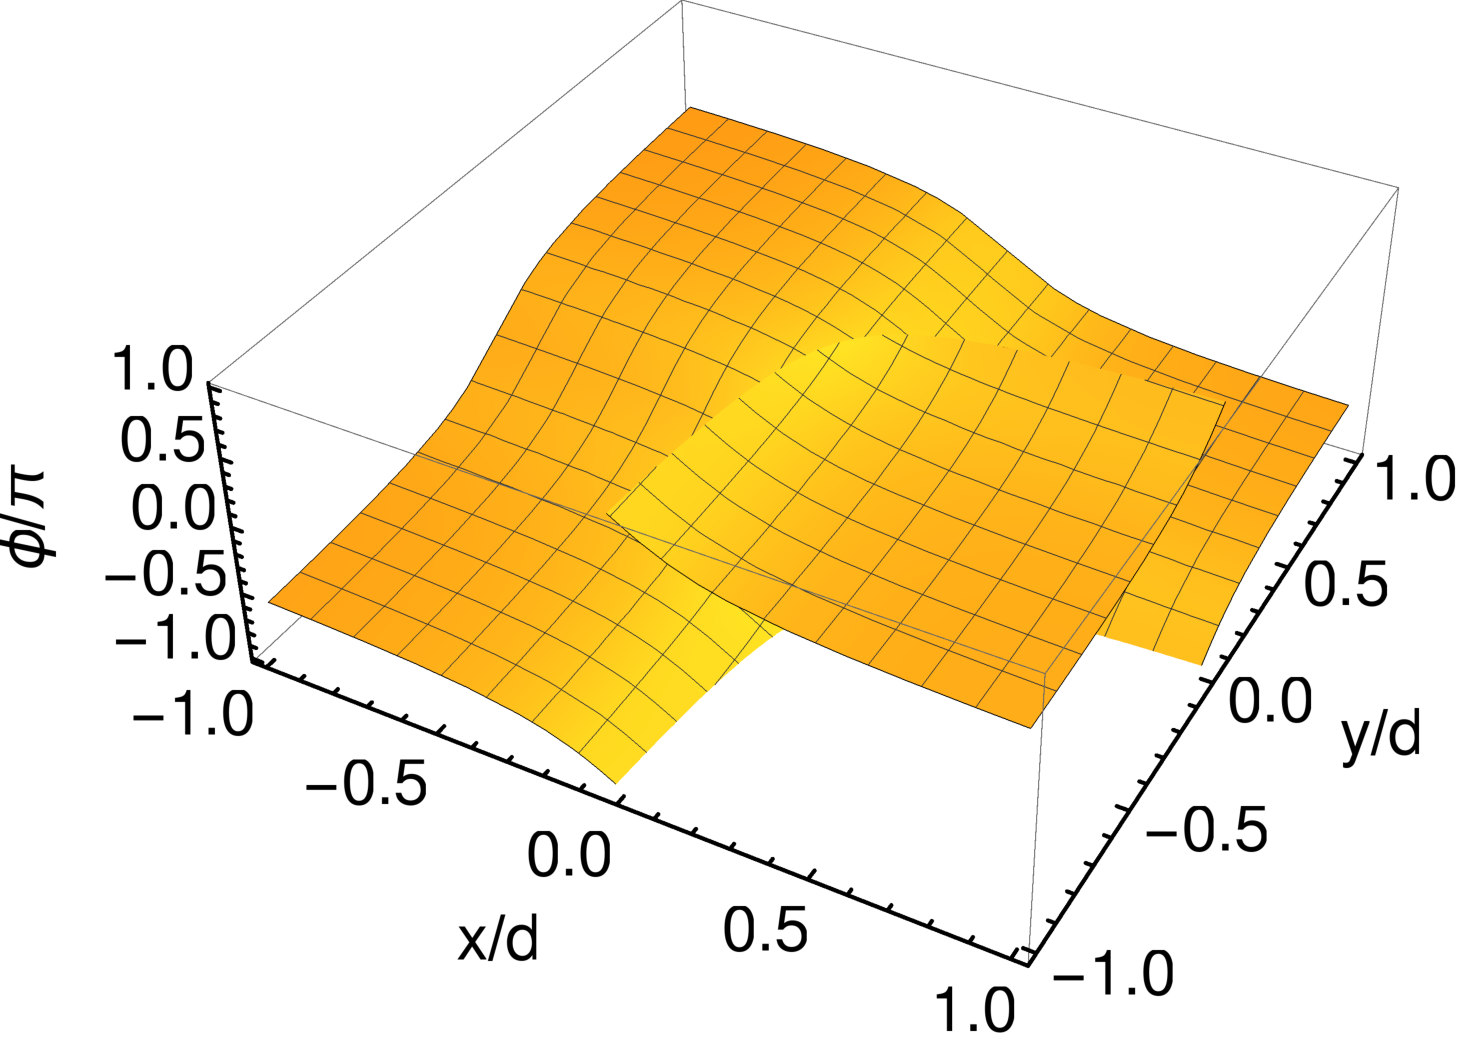
\includegraphics[width = 0.6\columnwidth]{Figures/fig_T_A_pot_arg.pdf}\\
    (c)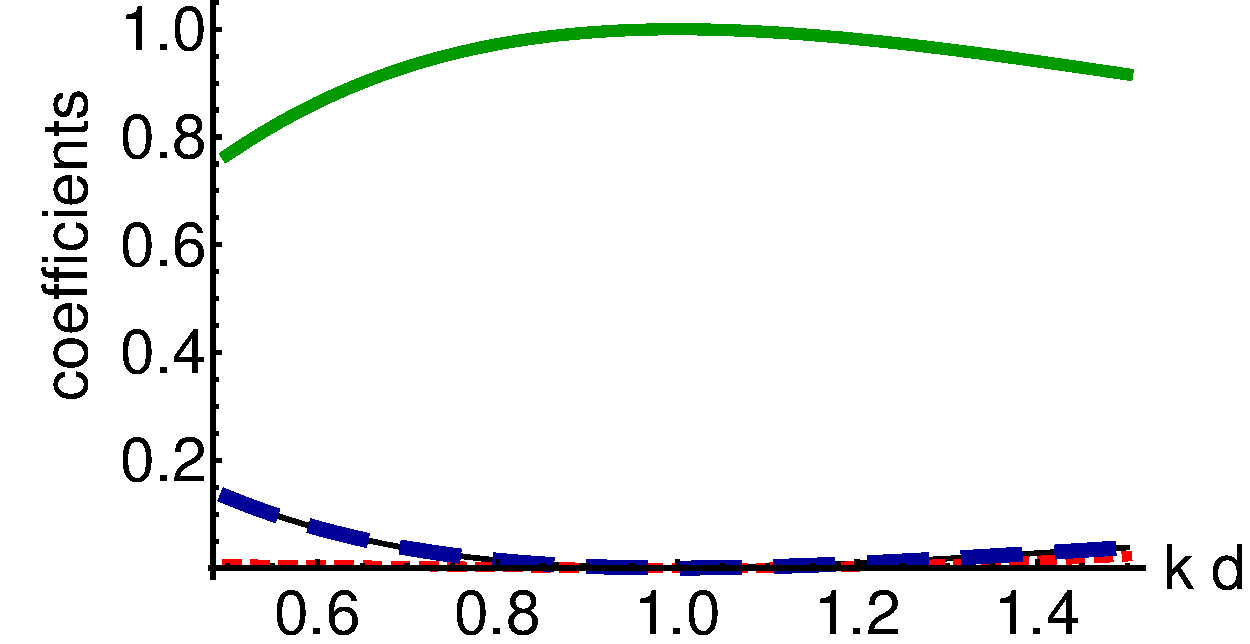
\includegraphics[width = 0.6\columnwidth]{Figures/fig_T_A_prob.pdf}
  \end{center}
  \caption{(Color online) One-way T-filter ($\cal{T/A}$, $\left|T^l\right|=1,T^r=R^l=R^r=0$) with  potential $V(x,y)=|V(x,y)|e^{i\phi(x,y)}$ set
  for $k_0 = 1/d$.
  (a) Absolute value $\left| V(x,y) \right|$;    (b) Argument $\phi(x,y)$;
  (c) Transmission and reflection coefficients:
  $\left| R^l \right|^2$ (black, solid line), $\left| T^l \right|^2$ (green, solid line),
  $\left| R^r \right|^2$ (blue, tick, dashed line), $\left| T^r \right|^2$ (red, dotted line). $V_0 = \hbar^2/(2m d^3)$.\label{fig_device_T_A}}
\end{figure}


%
%
%

\section{Designing potentials for asymmetric devices\label{sec:chapter1_examples}}

\begin{figure}
  \begin{center}
    (a) 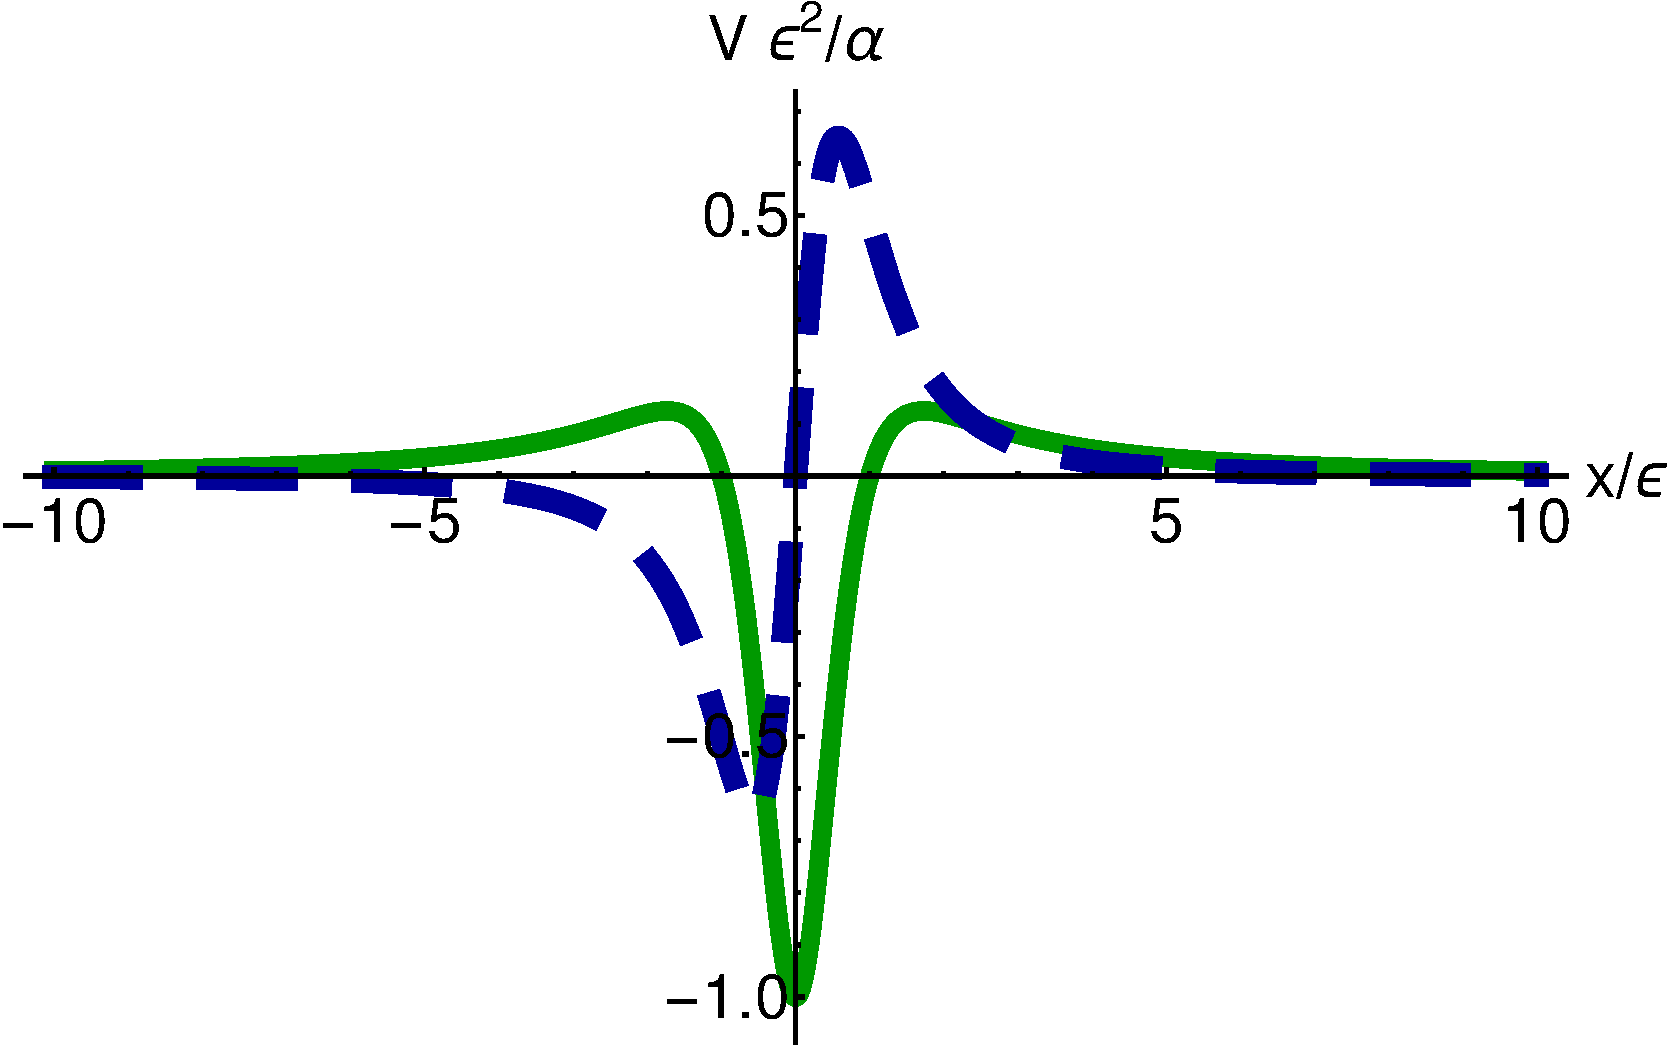
\includegraphics[width = 0.6\columnwidth]{Figures/fig_TR_T_local_pot.pdf}\\
    (b) 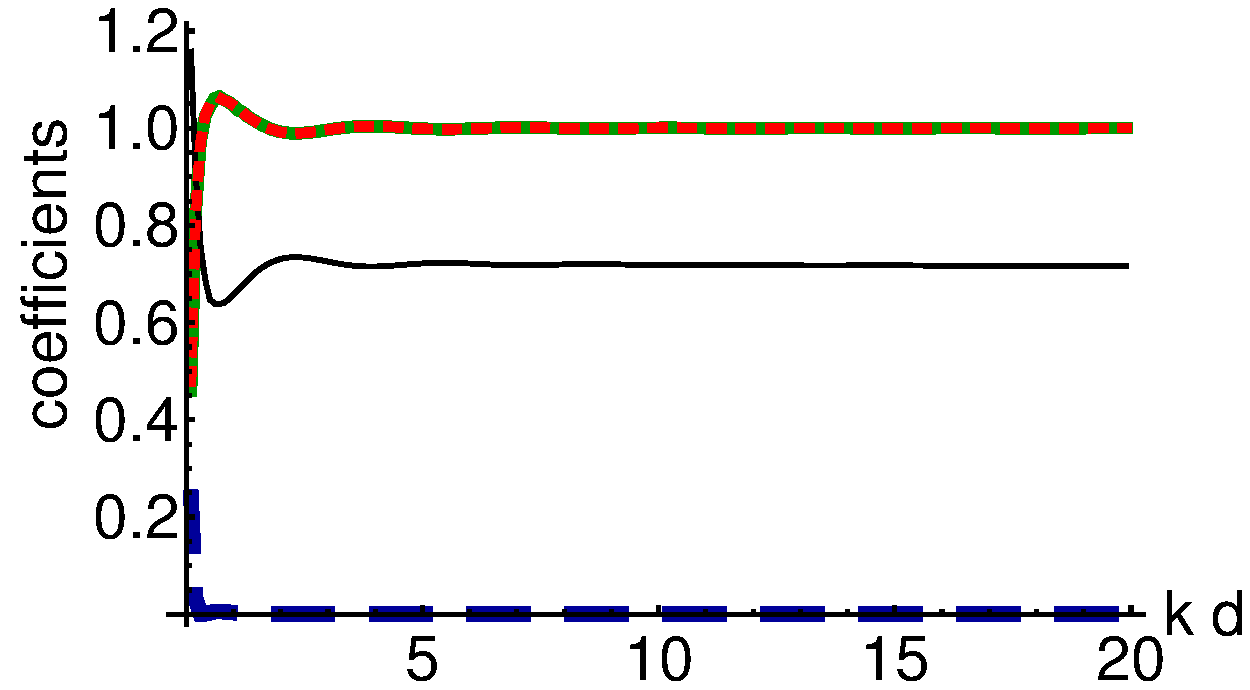
\includegraphics[width = 0.6\columnwidth]{Figures/fig_TR_T_local_prob_1.pdf}\\
    (c) 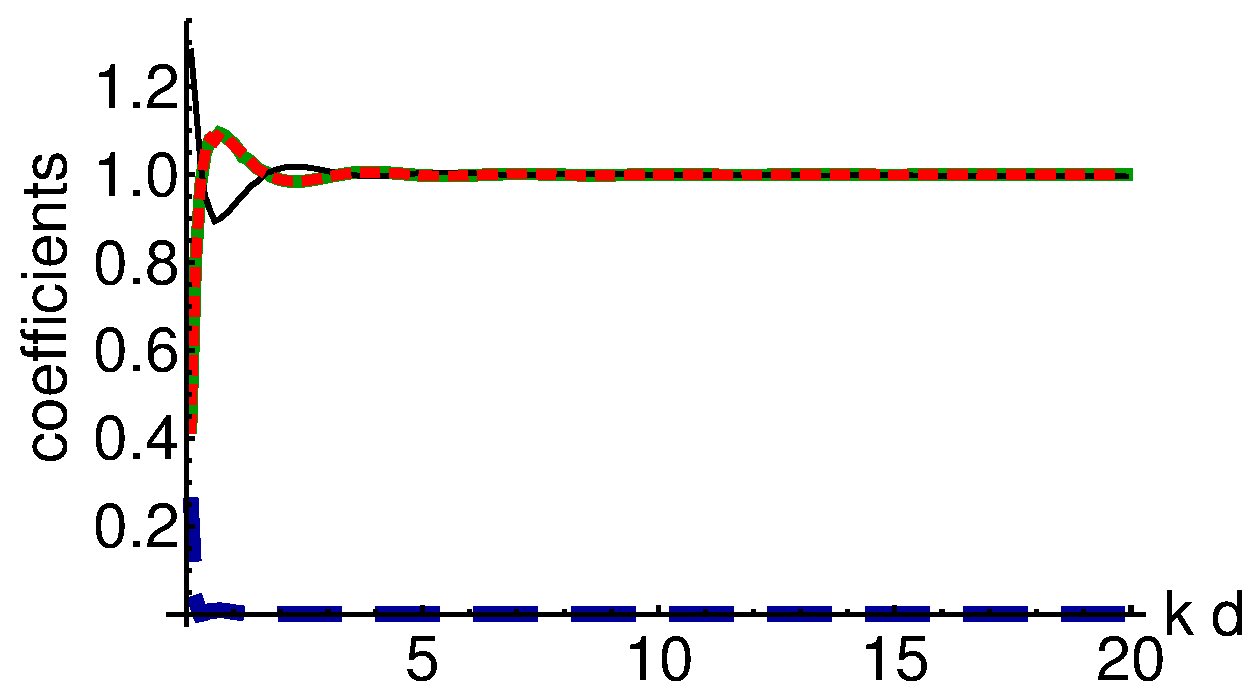
\includegraphics[width = 0.6\columnwidth]{Figures/fig_TR_T_local_prob_2.pdf}
  \end{center}
  \caption{\label{fig_reflector}(Color online) Transparent 1-way reflector with a local PT potential:
  (a) Approximation of the potential (\ref{num}), real part (green solid line), imaginary part (blue dashed line).
  (b,c) Transmission and reflection coefficients versus momentum $k d$;
  left incidence: $\left| R^l \right|^2$ (black, solid line), $\left| T^l \right|^2$ (green, solid line);
  right incidence: $\left| R^r \right|^2$ (blue, tick, dashed line), $\left| T^r \right|^2$ (red, dotted line, coincides with green, solid line).
  $\epsilon/d = 10^{-4}$.
  (b) $\alpha= 1.0 \hbar^2/(4\pi m)$ (c) $\alpha = 1.225 \hbar^2/(4\pi m)$
  (the black, solid line coincides here mostly with the red, dotted and green, solid lines).
  \label{fig_TR_T_local}}
\end{figure}


We will show  how to design non-local potentials
leading to the asymmetric devices.
For simplicity we look for  non-local potentials $V(x,y)$ with local support
that vanish  for $|x| >d$ and $|y| >d$.

To obtain the potentials for the asymmetric devices I follow an inverse scattering approach similar to \cite{Palao1998}. It starts by imposing an ansatz for the wavefunctions and the potential in the stationary Schr\"{o}dinger equation
%
\begin{eqnarray}
  \frac{\hbar^2k^2}{2m} \psi (x) = - \frac{\hbar^2}{2m} \frac{d^2}{dx^2} \psi (x)
  +\!\!\int_{-d}^d \!dy V(x, y) \psi(y).
  \label{Schroedinger}
\end{eqnarray}
%
The free parameters are fixed making use of the boundary conditions.
The form of the wavefunction incident from the left is
$\psi_l(x) = e^{i k x} + R^l e^{-i k x}$ for $x < -d$ and $\psi_l (x) = T^l e^{i k x}$ for $x > d$,
where  $k=p/\hbar$.
The wavefunction incident from the right is instead
$\psi_r(x) = e^{-ikx} T^r$ for $x < -d$ and $\psi_r (x) = e^{-i k x} + R^r e^{i k x}$ for $x > d$.

Our strategy is to assume  polynomial forms for the two wavefunctions in the interval $|x| < d$,
$\psi_l (x) = \sum_{j=0}^5 c_{l,j} x^j$ and $\psi_r (x) = \sum_{j=0}^5 c_{r,j} x^j$, and also a
polynomial ansatz of finite degree for the potential $V(x,y) = \sum_i \sum_j v_{ij} x^i y^j$.
Inserting these ansatzes in eq. (\ref{Schroedinger}) and from the conditions that $\psi_{l,r}$
and their derivatives must be continuous, all coefficients $c_{l,j}\,,c_{r,j}$ and $v_{ij}$ can be determined.
Symmetry properties of the potential can also be imposed via additional conditions on
the potential coefficients $v_{ij}$. For example we may use this method to obtain a one-way T-filter ($\cal{T/A}$) device (third device in table \ref{tab:chapter1_DevicesDescription}) with a nonlocal PT-pseudohermitian potential (symmetry VIII of table \ref{tab:chapter1_SymmetriesTable}) for a chosen wavevector $k = k_0$. The absolute value and argument of the resulting potential $V(x,y)$ are shown in figs. \ref{fig_device_T_A}(a) and \ref{fig_device_T_A}(b) together with its scattering coefficients as function of the incident wave vector, fig. \ref{fig_device_T_A}(c). As can be seen in fig. \ref{fig_device_T_A}(c) the imposed scattering coefficients are fulfilled exactly for the chosen wavevector. They are also satisfied approximately in a neighborhood of $k_0$. In the  Supplemental Material, Sec. II, we give further details about the construction of this potential and we work out other asymmetric devices of fig. \ref{fig:chapter1_cases}.
%
% ---------------------------------------- Asymmetric Reflection -----------------------------------
%
%
%
%

%
%%%%%%%%%%%%%%%%%%%%%%%%%%%%%%%%%%%%%%%%%%%%%%

%%%%%%%%%%%%%%%%%%%%%%%%%%%%%%%%%%%%%%%%%%%%%
%

\section{Extending the scattering asymmetry to a broad incident-momentum domain\label{sec:chapter1_extension}}
%
%
%
%
The inversion technique just described may be generalized
to extend the range of incident momenta for which the potential works by imposing additional
conditions and increasing correspondingly the number of parameters in the wavefunction ansatz,
for example we may impose that the derivatives of the  amplitudes,  in one or more orders,  vanish at $k_0$,
or  0/1 values for the coefficients not only at  $k_0$ but at a series of grid points $k_1$, $k_2$, ... $k_N$,
as in \cite{Brouard1994,Palao1998a,Palao1998,Muga2004}.

Here we put forward instead a method that provides a very broad working-window domain.
While we make formally use of the Born approximation, the exact numerical
computations demonstrate the robustness and accuracy of the approach to achieve that objective by
making use of an adjustable parameter in the potential. The very special role of the Born approximation in inverse problems has been
discussed and demonstrated in \cite{Snieder1990,Mostafazadeh2014,Horsley2015}.
Specifically we study a transparent one-way reflector ${\cal{TR/T}}$.
Our aim is now to find a local PT-symmetric potential such that asymmetric reflection results,
$T^l = T^r = 1, R^r = 0, |R^l|=1$ for a broad range of incident momenta. A similar goal
was pursued in \cite{Longhi2014} making use of a supersymmetric transformation,
without imposing $|R^l|=1$.

In the Born approximation and for a local potential $V(x)$, the reflection amplitudes take the simple form
%
\begin{eqnarray}
  R^l=-\frac{2\pi i m}{p}\langle -p|V|p\rangle,
  \;
  R^r=-\frac{2\pi i m}{p}\langle p|V|-p\rangle.
\end{eqnarray}
%
Defining the Fourier transform
%
\begin{eqnarray}
  \widetilde V (k) = \frac{1}{\sqrt{2\pi}} \int_{-\infty}^\infty dx \, V(x) e^{-i k x}
\end{eqnarray}
%
we get for $k=p/\hbar>0$:
%
\begin{eqnarray}
  R^l=-\frac{\sqrt{2\pi} i m}{k \hbar^2} \widetilde V (-2k),
  \;
  R^r=-\frac{\sqrt{2\pi} i m}{k\hbar^2} \widetilde V (2 k).
\end{eqnarray}
%
Assuming that the potential is local and PT-symmetrical, we calculate the transition coefficient
from them using generalized unitarity as
$|T|^2=1-{R^r}^*R^l$.

To build a ${\cal{TR/T}}$ device we demand:
$\widetilde V(k) = \sqrt{2\pi} \alpha k$ ($k < 0$) and $\widetilde V(k) = 0$ ($k \ge 0$).
By inverse Fourier transformation, this implies
%
\begin{eqnarray}
  V(x) &=&
  %-\alpha \frac{\partial}{\partial x} \left[P \frac{1}{x} + i \pi \delta(x) \right]
  %\nonumber\\
  %&=&
  -\alpha \frac{\partial}{\partial x} \lim_{\epsilon\to 0} \frac{1}{x - i \epsilon}
  = \alpha \lim_{\epsilon\to 0} \frac{1}{(x - i \epsilon)^2}
  \nonumber\\
  %&=& \alpha \lim_{\epsilon\to 0} \frac{(x + i \epsilon)^2}{(x^2 + \epsilon^2)^2}\\
  &=& \alpha \lim_{\epsilon\to 0} \left[\frac{x^2 - \epsilon^2}{(x^2 + \epsilon^2)^2} + i
  \frac{2 x\epsilon}{(x^2 + \epsilon^2)^2}\right],
  \label{num}
\end{eqnarray}
%
which is indeed a local, $PT$-symmetric potential for $\alpha$ real.
$\alpha$ is directly related to the reflection coefficient, within the Born approximation,
$R^l = 4 \pi i m \alpha/\hbar^2$. As the Born approximation may differ from exact results
we shall keep $\alpha$ as an adjustable parameter
in the following.

In a possible physical implementation, the potential in eq. (\ref{num}) will
be approximated by keeping a small finite $\epsilon>0$, see fig. \ref{fig_TR_T_local}(a).
%\begin{eqnarray}
%V(x) = \alpha \left[\frac{x^2 - \epsilon^2}{(x^2 + \epsilon^2)^2} + i
%\frac{2 x\epsilon}{(x^2 + \epsilon^2)^2}\right],
%\end{eqnarray}
%with a finite, small $\epsilon>0$.
Then, its Fourier transform is
$\widetilde V(k) = \sqrt{2\pi} \alpha k e^{\epsilon k}$ ($k < 0$) and $\widetilde V(k)=0$ ($k \ge 0$).
In figs. \ref{fig_TR_T_local}(b) and (c), the resulting coefficients for $\epsilon/d=10^{-4}$ and  two different values
of $\alpha$ are shown.  These figures have been calculated by
numerically solving the Schr\"odinger equation exactly.
% and demonstrate that
%$\alpha$ can indeed  be adjusted so that $\left| R^l \right|^2 \approx 1$.
Remarkably, the Born approximation contains all the information required to build the required potential shape
up to a global factor.  Such a prominent role of the Born approximation in inverse problems has been noted
in different applications \cite{Snieder1990,Mostafazadeh2014,Horsley2015}. For a range of $\alpha$, the potential gives $|R^r|\approx 0$, a nearly constant $|R^l|^2$, and
$|T^r|= |T^l|\approx1$  in a broad $k$-domain, see fig. \ref{fig_TR_T_local}(b). Adjusting  the value of $\alpha$, fig. \ref{fig_TR_T_local}(c),
sets $|R^l|\approx 1$ as desired.
%
%Remarkably, except for very low $k$,
%the potential is reflectionless from the right
%and provides full transmission independently of $\alpha$. As well, $|R^2|^2$ stays constant with respect to $k$ for different $\alpha$,
%so that that up to the adjustable parameter the Born approximation provides in fact the required potential shape, a surprising
%in inverse problems \cite{Snieder1990,Mostafazadeh2014,Horsley2015}.
%Figure \ref{fig_TR_T_local}(c) demonstrates that $\alpha$ can indeed be adjusted so that the  potential works
%as intended, i.e., as a transparent one-way reflector,  for a very broad range of $k$ values.

%
%
%
%
%
\section{Discussion\label{sec:chapter1_Discussion}}
%
%
Scattering asymmetries are necessary to develop technologically relevant devices such
as one-way mirrors, filters and  barriers, invisibility cloaks, diodes, or Maxwell demons.
So far much effort has been devoted to build and apply local PT-symmetric potentials but the possible scattering asymmetries with them are
quite limited. We find that six  device types with asymmetric scattering are possible
when imposing $0$ or $1$ scattering coefficients.
PT-symmetry can only realize one of them, but this symmetry  is just one among eight possible symmetries of complex non-local potentials.
The eight symmetries arise from the discovery that Klein's four-group
$\{1, \Pi, \Theta, \Theta\Pi\}$, combined with two possible relations among the Hamiltonian, its adjoint,
and the symmetry operators of the group, eqs. (1) and (2),
produce all possible  equalities among potential matrix elements after complex conjugation, coordinate inversion, the identity, and transposition.
In other words, to have all possible such equalities, the conventional definition of a symmetry $A$ in terms of its commutation with the Hamiltonian $H$ is not enough, and $A$-pseudohermiticity must be considered as well on the same footing.
Extending the concept of what a symmetry is for complex, non-local potentials is
a fundamental, far-reaching step of this work.
This group theoretical analysis and classification is not only esthetically pleasing, but also of practical importance, as it reveals
the underlying structure and span of the possibilities available in principle to manipulate the asymmetrical response of a potential
for a structureless particle.

We provide a potential for a One-way T-filter ($\mathcal{T}/\mathcal{A}$) and a PT potential for a transparent One-way reflector ($\mathcal{T}\mathcal{R}/\mathcal{T}$) that works in a broad domain of incident momenta. Although the present theory is for the scattering of quantum particles, the analogies between quantum physics and optics suggest to extend the concepts and results for optical asymmetric devices.
%
    % Asymmetric scattering by non-Hermitian potentials
%!TEX root = ../Thesis.tex
%Chapter 2

\chapter{$S$-matrix pole symmetries for non-Hermitian scattering Hamiltonians}
\label{Chapter2}
\lhead{Chapter 2. \emph{$S$-matrix pole symmetries for non-Hermitian scattering Hamiltonians}}

The complex eigenvalues of some non-Hermitian Hamiltonians, e.g. parity-time symmetric Hamiltonians, come in complex-conjugate pairs. We show that for non-Hermitian scattering Hamiltonians (of a structureless particle in one dimension) possesing one of four certain symmetries, the poles of the $S$-matrix eigenvalues in the complex  momentum plane are symmetric about the imaginary axis, i.e. they  are complex-conjugate pairs in complex-energy plane. This applies even to states which are not bounded eigenstates of the system, i.e. antibound or virtual states, resonances, and antiresonances. Example potentials with such symmetries are constructed and their pole structures and scattering properties are calculated.
%
\newpage
%
\section{Introduction}

Much work on non-hermitian (NH) physics has focused on PT-symmetric Hamiltonians, as they may have a purely real spectrum \cite{Bender1998}. More recently, other NH and non-PT Hamiltonians, have been shown to hold real eigenvalues \cite{Nixon2016,Chen2017,Yang2017}. Work on scattering by PT-symmetric potentials was at first rather scarce \cite{Muga2004,Ruschhaupt2005,Cannata2007,Znojil2015}. However, scattering has been later investigated intensely in connection with spectral singularities and reflection asymmetries for left or right incidence (i.e. unidirectional invisibility) \cite{Mostafazadeh2009,Longhi2014,Mostafazadeh2013}, in most cases restricting the analysis to local potentials. As was shown in chapter \ref{Chapter1}, different devices with asymmetrical scattering responses (i.e., with different transmission and/or reflection for right and left incidence in a 1D setting) are possible if one makes use of non-local potentials. Chapter \ref{Chapter1} provides the selection rules for the transmission and reflection coefficient asymmetries based on eight basic Hamiltonian symmetries. Four of theses symmetries are a standard conmutation between a symmetry operator $A$ and the Hamiltonian, eq. \eqref{eq:chapter1_symmetry}, and the other four are $A$-pseudohermicity, \eqref{eq:chapter1_pseudoSymmetry}. $A$ is an element of the Klein 4-group $\mathbf{K}_4 = \left\{1,\Pi,\Theta,\Theta\Pi\right\}$.

A set of works by A. Mostafazadeh \cite{Mostafazadeh2002,Mostafazadeh2002a,Mostafazadeh2002b} gives the sufficient and necesary conditions for hamiltonians with a discrete spectrum to have real or complex conjugate pairs of eigenvalues. Hamiltonians satisying eq. \eqref{eq:chapter1_pseudoSymmetry} for a hermitian linear operator $A$, \textit{i.e.} $A$-pseudohermicity have a spectrum in which the eigenvalues come in complex conjugate pairs, some of them can even be real-valued. Moreover, the results of \cite{Mostafazadeh2002b} show that if a Hamiltonian conmutes with a hermitian antilinear operator, then there will exist a hermitian linear operator $A$ for which the Hamiltonian is $A$-pseudohermitian and, therefore, it will have complex conjugate pairs of eigenvalues. However, an aspect uncovered in refs. \cite{Mostafazadeh2002,Mostafazadeh2002a,Mostafazadeh2002b} is that when the Hamiltonian is $A$-pseudohermitian, the poles of the scattering matrix can have the same properties as the discrete spectrum, they can also come in complex conjugate pairs.

This chapter aims at extending the results in chapter \ref{Chapter1} and refs. \cite{Mostafazadeh2002,Mostafazadeh2002a,Mostafazadeh2002b} in several directions:

i) I will provide an alternative characterization of the 8 symmetries formed by the elements of the Klein 4-group and the relations \eqref{eq:chapter1_symmetry}, \eqref{eq:chapter1_pseudoSymmetry} in terms of the invariance of $H$ with respect to the action of superoperators.

ii) Moreover,
four of these eight symmetries imply the same
type of pole structure of $S$-matrix eigenvalues in the complex momentum plane that was found for PT symmetry \cite{Muga2004},
namely, zero-pole correspondence at complex-conjugate points, and poles on the imaginary axis or forming symmetrical pairs with respect to the imaginary
axis. This configuration with poles located on the imaginary  axis or as symmetrical pairs has some important consequences. In particular, it provides stability of the real energy eigenvalues with respect to parameter variations of the potential. While a simple pole on the imaginary axis can move along that axis when a parameter is changed, it cannot move off this axis (since this would violate the pole-pair symmetry) or bifurcate. The formation of pole pairs occurs near special  parameter values for which two poles on the imaginary axis collide. When the poles are mapped to the energy complex plane $E = p^2/2m$, they have the same symmetry structure of complex conjugate pairs as the discrete eigenvalues of $A$-pseudohermitian Hamiltonian, which expands the results of refs. \cite{Mostafazadeh2002,Mostafazadeh2002a,Mostafazadeh2002b}.

The remainder of the chapter is organized as follows. In section \ref{sec:chapter2_super} I characterize the symmetry operations defined in chapter \ref{Chapter1} as the invariance of the Hamiltonian with respect to the action of eight linear or antilinear superoperators. In section \ref{sec:chapter2_SPoles} I discuss the physical consequences of the symmetries in the pole structure of the scattering matrix eigenvalues. Four symmetries are shown to lead to complex poles corresponding to real energies or conjugate (energy) pairs. This result generalizes what was found in refs. \cite{Mostafazadeh2002,Mostafazadeh2002a,Mostafazadeh2002b}. In section \ref{sec:chapter2_separablePotentials} I exemplify the general results with separable potentials exhibiting parity-pseudohermiticity and time-reversal symmetry. These are the two non-trivial symmetries of the four (in the sense that the other two, hermiticity and PT-symmetry, are already well discussed). In section \ref{sec:chapter2_Discussion} I discuss and summarize the results.
%
\begin{landscape}
  \begin{table}
    \centering
    \caption{Symmetries of the Hamiltonian with respect to the commutativity or pseudohermiticity of $H$ with the elements of $\mathbf{K}_4$ (column 2) in terms of the action of superoperators $\mathcal{L}$ on the potential $V$ in coordinate (Column 4) or momentum (Column 6) representation. This table follows the same code convention with roman numbers for the symmetries as chapter \ref{Chapter1} and can be seen as an extension of table \ref{tab:chapter1_SymmetriesTable} incorporating the superoperator formalism
    \vspace*{.2cm}
    \label{tab:chapter2_Symmetries}}
    \scalebox{1}{
    \begin{tabular}{ccccccccccc}
      \hline
      \hline\\
      (1)&(2)&(3)&(4)&(5)&(6)&(7)&(8)&(9)&(10)&(11)
      \\
      Code & Symmetry&  $\la x|V|y\ra$ & ${\cal{L}}$(coord)& $\la p|V|p'\ra$ & ${\cal L}$(momentum) &$\la p|S|p'\ra$ & $T^l$ & $T^r$ & $R^l$& $R^r$
      \\
      \hline
      I & $1H=H1$ &   $\la x|V|y\ra$ & ${ 1}$ &$\la p|V|p'\ra$ &${ 1}$& $\la p|S|p'\ra$ & $T^l$ & $T^r$ & $R^l$ & $R^r$
      \\
      II & $1H=H^\dagger 1$ &  $\la y|V|x\ra^*$ & ${\cal TC}$& $\la p'|V|p\ra^*$ &${\cal T'C'}$&$\la p|\widehat{S}|p'\ra$ & $\widehat{T}^l$& $\widehat{T}^r$ & $\widehat{R}^l$ & $\widehat{R}^r$
      \\
      III & $\Pi H=H\Pi$ &  $\la -x|V|-y\ra$ &${\cal I}$&  $\la -p|V|-p'\ra$ &${\cal I'}$&$\la -p|S|-p'\ra$ & $T^r$ & $T^l$ & $R^r$ & $R^l$
      \\
      IV & $\Pi H=H^\dagger \Pi$ &  $\la -y|V|-x\ra^*$ &${\cal CTI}$& $\la -p'|V|-p\ra^*$ &${\cal C'T'I'}$& $\la -p|\widehat{S}|-p'\ra$ & $\widehat{T}^r$ & $\widehat{T}^l$ & $\widehat{R}^r$ & $\widehat{R}^l$
      \\
      V & $\Theta H=H\Theta$ &  $\la x|V|y\ra^*$&${\cal C}$& $\la -p|V|-p'\ra^*$ &${\cal I'C'}$& $\la -p'|\widehat{S}|-p\ra$ & $\widehat{T}^r$ & $\widehat{T}^l$ & $\widehat{R}^l$& $\widehat{R}^r$
      \\
      VI & $\Theta H=H^\dagger\Theta$ &  $\la y|V|x\ra$&${\cal T}$& $\la -p'|V|-p\ra$ &${\cal I'T'}$& $\la -p'|S|-p\ra$ & $T^r$& $T^l$ & $R^l$& $R^r$
      \\
      VII & $\Theta\Pi H=H\Theta \Pi$ &  $\la -x|V|-y\ra^*$ &${\cal IC}$& $\la p|V|p'\ra^*$ &${\cal C'}$& $\la p'|\widehat{S}|p\ra$ &$\widehat{T}^l$& $\widehat{T}^r$ & $\widehat{R}^r$& $\widehat{R}^l$
      \\
      VIII& $\Theta\Pi H=H^\dagger \Theta \Pi$ &  $\la -y|V|-x\ra$ &${\cal IT}$& $\la p'|V|p\ra$ &${\cal T'}$& $\la p'|S|p\ra$ & $T^l$ & $T^r$ & $R^r$ & $R^l$
      \\
      \hline
      \hline
    \end{tabular}
    }
  \end{table}
\end{landscape}
% -------------------------------------------------------------------------------------------------


\section{Superoperator formalism\label{sec:chapter2_super}}

The eight symmetries discussed in chapter \ref{Chapter1}, which are listed again in Table \ref{tab:chapter2_Symmetries} may also be regarded as the invariance of the Hamiltonian with respect to
transformations represented by superoperators ${\cal L}$ \cite{Simon2018} defined by
%
\begin{equation}
	\mathcal{L}(H)=
	\begin{cases}
		A^\dagger H A &  \text{I, III,V,VII} \\
		A^\dagger H^\dagger A &\text{II, IV, VI, VIII}
		\end{cases}.
\end{equation}
%
This definition of the superoperator action is independent of the representation we use, but its realization in coordinates or momenta representation in terms of the operations of complex conjugation $\mathcal{C}$, transposition $\mathcal{T}$, and inversion (sign reversal of momentum or position) $\mathcal{I}$ is different. In coordinate representation, these superoperators take the following forms (see column 3 in Table \ref{tab:chapter2_Symmetries}),
%
\begin{align}
	1 H&=\int\!\!\int |x\ra \la x|H|y\ra\la y| dx dy,
	\nonumber\\
	{\cal T} (H) &=\int\!\!\int |x\ra \la y|H|x\ra\la y| dx dy,
	\nonumber\\
	{\cal C} (H)&=\int\!\!\int |x\ra \la x|H|y\ra^*\la y| dx dy,
	\nonumber\\
	{\cal I} (H)&=\int\!\!\int |x\ra \la -x|H|-y\ra\la y| dx dy,
	\label{eq:chapter2_superoperatorsPosition}
\end{align}
%
while in momentum representation, these superoperators are
%
\begin{align}
	1 H&=\int\!\!\int |p\ra \la p|H|q\ra\la q| dp dq,
	\nonumber\\
	{\cal T}' (H) &=\int\!\!\int |p\ra \la q|H|p\ra\la q| dp dq,
	\nonumber\\
	{\cal C}' (H)&=\int\!\!\int |p\ra \la p|H|q\ra^*\la q| dp dq,
	\nonumber\\
	{\cal I}' (H)&=\int\!\!\int |p\ra \la -p|H|-q\ra\la q| dp dq.
	\label{eq:chapter2_superoperatorsMomentum}
\end{align}
%
Adopting the trace inner product for linear operators $F$ and $G$
%
\begin{equation}
  \langle\langle F|G\rangle\rangle={\rm{tr}} F^\dagger G
  \label{eq:chapter1_innerProduct}
\end{equation}
%
we can show that all superoperators (also the primmed ones) and their products ${\cal L}$ are either unitary (for ${\cal L}=1,{\cal T},{\cal I},{\cal TI}$), or antiunitary (for ${\cal L}={\cal C}, {\cal CT},{\cal CI},{\cal CTI}$), with respect to the inner product as defined by
%
\begin{eqnarray}
	\langle\langle {\cal L}F| {\cal L}G\rangle\rangle&=& \langle\langle F| G\rangle\rangle\;\;\;  ({\cal L}\; {\rm unitary}),
	\\
	\langle\langle {\cal L}F| {\cal L} G\rangle\rangle&=& \langle\langle  F| G\rangle\rangle^*\;\;\;  ({\cal L}\; {\rm antiunitary}).
\end{eqnarray}
%
They all satisfy ${\cal L}{\cal L}^\dagger={\cal L}^\dagger {\cal L}=1$
where the adjoints are defined differently for linear or antilinear superoperators,
\begin{eqnarray}
	\langle\langle F| {\cal L}^\dagger G\rangle\rangle&=& \langle\langle {\cal L} F| G\rangle\rangle\;\;\;  ({\cal L}\; {\rm unitary}),
	\\
	\langle\langle F| {\cal L}^\dagger G\rangle\rangle&=& \langle\langle {\cal L} F| G\rangle\rangle^*\;  ({\cal L}\; {\rm antiunitary}).
\end{eqnarray}
%
Moreover the eight superoperators  satisfy ${\cal L}^\dagger={\cal L}$.

The set $\{1, \cal{I,T,C,CT,TI,IC,CTI}\}$ (and the primmed ones) forms the elementary abelian group $E8$ \cite{Rose2009}. This is a homocyclic group, namely, the direct product of isomorphic
cyclic groups of order 2 with generators $\cal{C,T,I}$. Only for the subgroup $\{1, \cal{I,CT,CTI}\}$ the superoperators have the same representation-independent form in terms of complex conjugation, transposition and inversion in momentum and position bases.

A direct application of the superoperator framework is the generalization of Wigner's
formulation of symmetries \cite{Wigner1959}. He associated symmetry transformations to unitary or antiunitary operators preserving the (Hilbert space) inner product, namely the ``transition probabilities'' $|\expval{A\psi,A\phi}|^2=|\expval{\psi,\phi}|^2$.
For general states described by density operators $\rho_1,\rho_2$, transition probabilities are computed as $\la\la \rho_1|\rho_2\ra\ra$
and the transformations described by the unitary or antiunitary superoperators preserve the
transition probability. Hamiltonian symmetries are, within the conventional Wigner scheme, the  symmetry transformations that leave the Hamiltonian invariant ($A^\dagger H A=H$, so that $A$ and $H$ commute). Here the Hamiltonian symmetry is more broadly defined  as
the invariance ${\cal L}H=H$, which includes transformations  beyond the conventional scheme.

\section{S-matrix pole structure}
\label{sec:chapter2_SPoles}
%
In refs. \cite{Mostafazadeh2002,Mostafazadeh2002a,Mostafazadeh2002b}, Mostafazadeh derived the sufficient and necessary conditions of diagonalizable Hamiltonians with a discrete spectrum for having a spectrum made of real eigenvalues and complex-conjugate pairs of eigenvalues. The condition was that the Hamiltonian had to be $A-$pseudohermitian with respect to a hermitian linear operator $A$ or commute with a hermitian antilinear operator $B$. In fact, the two conditions are equivalent \cite{Mostafazadeh2002b}: If a Hamiltonian is $A$-pseudohermitian one can find a hermitian antilinear $B$ that commutes with $H$ and viceversa. In this section I generalize the results in \cite{Mostafazadeh2002,Mostafazadeh2002a,Mostafazadeh2002b} to scattering Hamiltonians. I show, for the symmetry operators in the Klein 4-group, that the poles of the $S-$matrix have the same structure as the eigenvalues of the discrete spectrum, as described in \cite{Mostafazadeh2002,Mostafazadeh2002a,Mostafazadeh2002b}, when the Hamiltonian satisfies symmetries V and VII of table \ref{tab:chapter2_Symmetries}, \textit{i.e.}, eq. \eqref{eq:chapter1_symmetry} for $A$ antiunitary ($A = \Theta,\Pi\Theta$), or symmetries II and IV of table \ref{tab:chapter2_Symmetries}, \textit{i.e.}, eq. \eqref{eq:chapter1_pseudoSymmetry} for A unitary ($A = 1,\Pi$).


In section \ref{sec:chapter1_ScattFormalism} we introduced the scattering matrix ($S$-matrix) formalism, which was used to derive the results of chapter \ref{Chapter1} regarding the scattering coefficients. It was possible to decompose the $S$-matrix into the on-the-energy-shell matrices $\sf{S}$ for real and positive momentum in terms of transmission and reflection amplitudes for right
and left incidence, see eq. \eqref{eq:chapter1_onShellMatrix}. The $\sf{S}$ matrix contains the scattering amplitudes for incoming wave packets with well defined momentum being scattered into states with the same kinetic energy and reflected and transmitted components. The on-shell scattering matrix $\mathsf{S}$ allowed us to obtain the generalized unitary relations \eqref{eq:chapter1_SMatrixUnitarityGeneralized} in terms of the scattering amplitudes \eqref{eq:chapter1_unitarityCoefficients}. For negative $p$ the matrix elements of $\mathsf{S}$ give the amplitudes of scattering states with a pure outgoing plane wave towards the right or the left. Moreover we assume, as it is customary, that the amplitudes may be continued analytically beyond the real axis. The existence of a continuation on a complex plane domain depends on decay properties of the potentials and may
be checked for each potential.
The analytical continuation is indeed possible for the model potentials of the following section.

We will look for the poles of the $S$-matrix in the eigenvalues of its on shell decomposition $\mathsf{S}$. The eigenvalues of $\sf{S}$ can be calculated from the transmission and reflection amplitudes as
%
\begin{equation}
	S_j=\frac{(T^l+T^r)+(-1)^j[(T^l-T^r)^2+4R^lR^r]^{1/2}}{2}
	\label{eq:chapter2_SEigenvalues}
\end{equation}
%
for $j=1,2$, and of course there is a similar expression for $\widehat{S}_j$ (The scattering matrix for the adjoint Hamiltonian) with hatted amplitudes.
In general they satisfy the relations \cite{Muga2004},
%
\begin{equation}\label{eq:chapter2_pam1}
	S_j(p)=\widehat{S}_j^*(-p^*)\,,
\end{equation}
%
and
%
\begin{equation}\label{eq:chapter2_pam2}
	\widehat{S}_j^*(p^*)S_j(p)=1\,.
\end{equation}
%
Combining Eqs. (\ref{eq:chapter2_pam1}) and (\ref{eq:chapter2_pam2}) gives
%
\begin{equation}\label{eq:chapter2_pam3}
	S_j(p)=S^{-1}_j(-p)\,.
\end{equation}
%
Equation \eqref{eq:chapter2_pam3} is remarkable since it reveals the presence of a pole (zero) at $-p$ if there is a zero (pole) at $p$.
%
If the following relations are fulfilled,
%
\begin{eqnarray}
	T^{r,l}(p)&=&\widehat{T}^{r,l}(p)\; {\rm or}\; T^{r,l}(p)=\widehat{T}^{l,r}(p),
	\label{ts}
	\\
	R^{r,l}(p)&=&\widehat{R}^{r,l}(p)\; {\rm or}\; R^{r,l}(p)=\widehat{R}^{l,r}(p),
	\label{rs}
\end{eqnarray}
%
then
%
\begin{equation}
	S_j(p)=\widehat{S}_j(p),
\end{equation}
%
which together with Eq. \eqref{eq:chapter2_pam1} gives
%
\begin{equation}
	S_j(p)=S_j^*(-p^*).
	\label{eq:chapter2_PoleSymmetry}
\end{equation}
%}
In plain language, Eq. \eqref{eq:chapter2_PoleSymmetry} tells that if Eqs. (\ref{ts}) and (\ref{rs}) are satisfied,  the poles and zeros of $S_j$ must be symmetrically distributed with respect to the imaginary axis of momentum complex plane. Combined with Eq. (\ref{eq:chapter2_pam3})
this also means that each pole has a symmetrical zero with respect to the real axis. This symmetrical distribution of poles and zeros is the same as in the Hermitian case (see Fig. \ref{fig:DiagramPoles}),
%end red
the only difference being the possibility
of finding pairs of symmetrical poles in the upper complex plane when $H\neq H^\dagger$. They represent normalizable ``bound states
with complex energies''. When they  are not present, the discrete spectrum becomes purely real.

According to Table \ref{tab:chapter2_Symmetries},  Eqs. (\ref{ts}) and (\ref{rs}) are fulfilled
for symmetries  II (hermiticity), VII (PT-symmetry), IV (parity pseudohermiticity),
and V (time-reversal invariance). Thus, Hamiltonians having these symmetries have their $S-$matrix poles symmetrically distributed around the imaginary axis. For local potentials the last two symmetries coalesce with the first two well-known
cases \cite{Ruschhaupt2017}, namely,
IV becomes equivalent to PT-symmetry, and V becomes equivalent to hermiticity. For non-local potentials, though, these symmetries
correspond to genuinely distinct properties. In the following section we shall demonstrate this fact with potentials that are
either purely parity-pseudohermitian (and not PT-symmetrical), or time-reversal invariant but not Hermitian.
%


\begin{figure}[h]
  \centering
  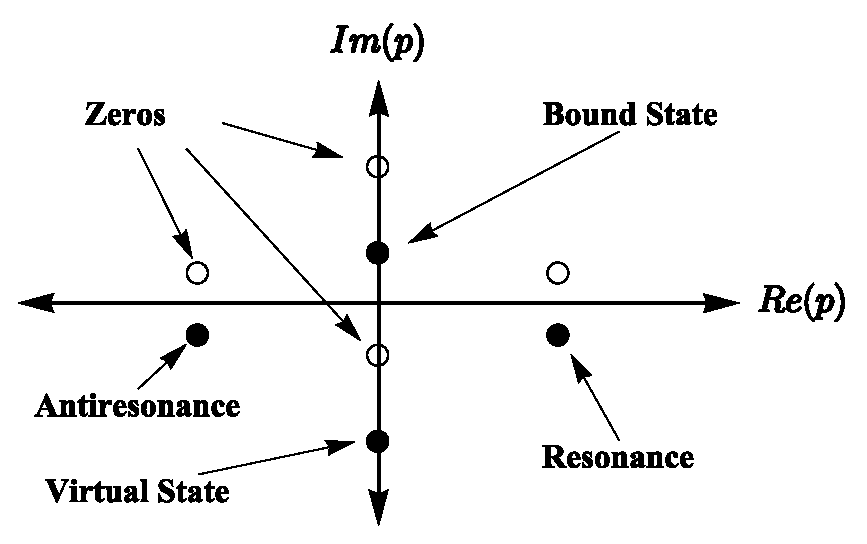
\includegraphics[width=0.5\linewidth]{Figures/DiagramPoles.eps}
  \caption{Example of configuration of poles (filled circles) and zeros (empty circles) of the $S$-matrix eigenvalues in the complex momentum plane for hermitian Hamiltonians.  Poles in the upper half plane ($\operatorname{Im}(p) > 0$) correspond to bound eigenstates of the Hamiltonian, i.e. localized states with negative energy. Poles in the lower half plane correspond to  virtual states ($\operatorname{Re}(p) = 0$), resonances ($\operatorname{Re}(p) > 0$) and antiresonances ($\operatorname{Re}(p)<0$). The singularities with negative imaginary part correspond to states that do not belong to the Hilbert space since they are not normalizable. However, they can produce observable effects in the scattering amplitudes, in particular when they approach the real axis. The pole structure of symmetries IV, V, and VII, see Table \ref{tab:chapter2_Symmetries},
  is similar, but pole pairs are also possible in the upper half-plane.}
  \label{fig:DiagramPoles}
\end{figure}

\section{Separable Potentials}
\label{sec:chapter2_separablePotentials}
%
%
In order to illustrate and test the theoretical concepts that we have discussed, in particular the
symmetrical configuration of poles with respect to the imaginary axis in the complex momentum plane for certain Hamiltonian symmetries, we will use some solvable toy models consisting on rank-one separable potentials.
Separable potentials are quite useful models as a solvable approximation to realistic ones, in particular in nuclear, atomic and molecular physics \cite{Popov2019}.
Often they lead to explicit expressions
for wave functions or scattering amplitudes, so they are used to test concepts and new methods.
They are also instrumental in learning about different dynamical phenomena (for example transient effects, short-time and long-time behavior, or anomalous decay laws)  and their relation to complex-plane singularities
\cite{Muga1990,Muga1996,Muga1996a,Muga1998}. Their simplest version takes the form
$|\chi\ra V_0\la\chi|$ for some  $\chi$.   In particular, with a complex $V_0$,
they have been used to examine anomalous (negative) time delays caused by  crossing of zeroes of the $S$-matrix eigenvalues or $S$-matrix elements across the momentum real axis \cite{Muga1998a}.

In this work we consider the simple structure
$V=V_0 \ketbra{\phi}{\chi}$, with $V_0$ (potential strength) real, and conveniently chosen normalised states $\ket{\phi}$, $\ket{\chi}$.
The aim of this section is to demonstrate the formal results of the previous section without attempting to simulate any specific systems, but we note that separable, NH potentials are instrumental to model nuclear reactions, in particular  by increasing the rank (number of separable terms) \cite{Hlophe2017}.
Separable NH potentials also provide solvable approximations to nonlocal NH potentials that arise naturally in quantum optics to describe the interaction of a ground state atom with a laser beam \cite{Ruschhaupt2004a}.

I proceed to look for the poles of the ${\sf S}$ matrix in the following way. Since the scattering amplitudes in ${\sf S}$ are simply related to matrix elements of $T_{op}(z)$ (eq. \eqref{eq:chapter1_transitionOperator_definition}) in momentum representation, see eq. \eqref{eq:chapter1_amplitudesFromTOperator}, the singularities in the scattering amplitudes and the eigenvalues of ${\sf S}$ will come from the singularities of $T_{op}(z)$ \cite{Muga1996}. For a separable potential, the transition operator $T_{op}$ can be written (see Appendix \ref{Appendix:SeparablePotentials_TransitionOperator}) as
%
\begin{equation}
	T_{op}=\frac{V_{0}}{1-V_{0} Q_{0}(E)} \ketbra{\phi}{\chi},
  \label{eq:chapter2_TransitionOperatorSeparablePotential}
\end{equation}
%
where $Q_{0}(E)=\bra{\chi}(E-H_0)^{-1}\ket{\phi}$ and $H_{0}=p^{2}/(2m)$. Therefore, the singularities (poles) of ${\sf S}$ are found by solving
%
\begin{eqnarray}
	Q_{0}(E)V_{0} = 1,
	\label{eq:chapter2_roots}
\end{eqnarray}
%
Once $Q_{0}(E)$  is calculated, the transmission and reflection amplitudes can be found from \eqref{eq:chapter1_amplitudesFromTOperator} using the momentum representation of $\ket{\phi}$ and $\ket{\chi}$ (see Appendix \ref{Appendix:SeparablePotentials_AmplitudesAndEigenvaluesofS}).

In the following subsections I will build a Hamiltonian with symmetry V (time reversal) and another one with symmetry IV (parity pseudohermicity) and illustrate the symmetries of the $S$ matrix poles in momentum complex plane.
%
\subsection{Time-reversal symmetric potential}
%
%
\begin{figure}[h]
  \centering
	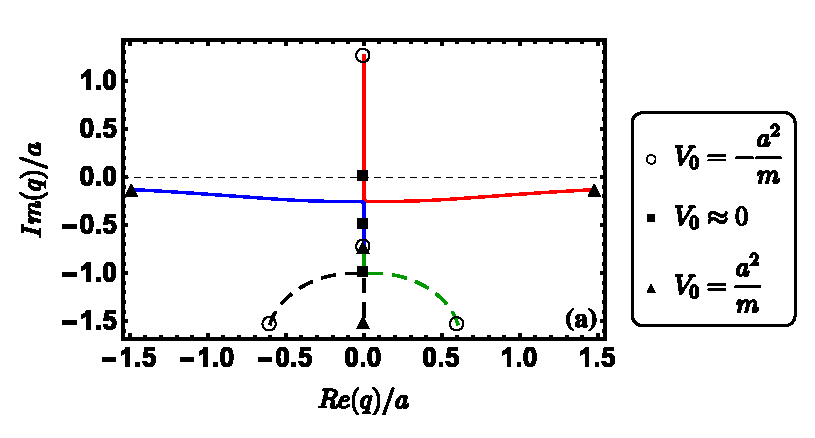
\includegraphics[width=0.75\linewidth]{Figures/VSymEigenvalsVaryingV0_Momentum.eps}
	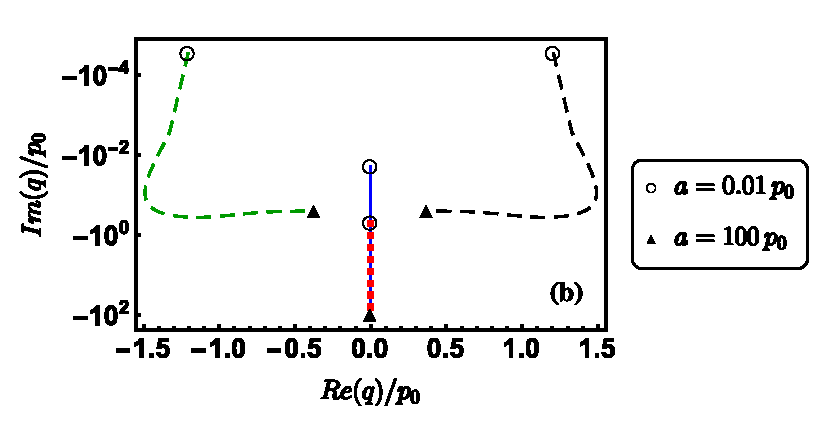
\includegraphics[width=0.75\linewidth]{Figures/VSymEigenvalsVaryingA_Momentum_Log.eps}
	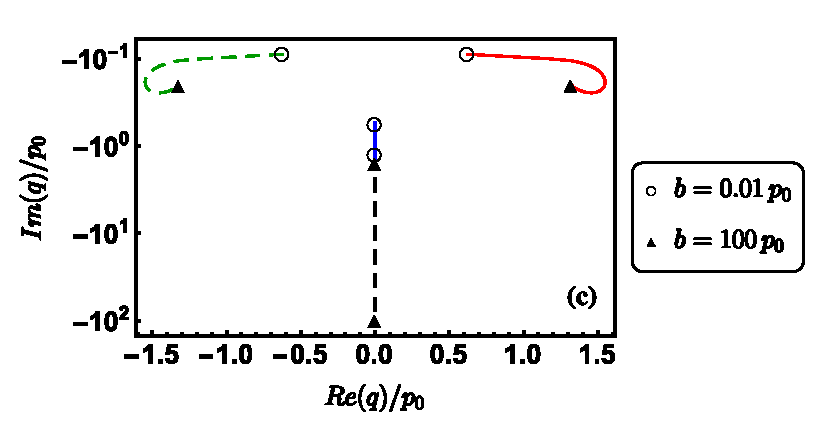
\includegraphics[width=0.75\linewidth]{Figures/VSymEigenvalsVaryingB_Momentum_Log.eps}
	\caption{ Poles and pole trajectories of time-reversal symmetric potential \eqref{TRpot} for (a) varying $V_0$ with $a=2 b$; (b) varying $a$ with $b=0.5\, p_0$, $V_0>0$; and (c) varying $b$ with $a=p_0$,
	$V_0>0$. At pole collisions we connect each of the incoming trajectories with a different emerging trajectory but the choice of outgoing branch  is arbitrary since the two colliding poles lose their identity.}
	\label{fig:VSymEigenvals}
\end{figure}

We start with an example of a separable potential which only satisfies symmetry V (apart from the trivial symmetry I). The normalised vector $\ket{\chi}$, is given in position and momentum representation as
%
\begin{eqnarray}
	\braket{x}{\chi}&=&\sqrt{\frac{a}{\hbar}} e^{-a \left| x \right|/\hbar},
	\nonumber \\
	\braket{p}{\chi}&=& \sqrt{\frac{2 a^3}{\pi}} \frac{1}{p^2+a^2}.
\end{eqnarray}
%
We choose $\ket{\phi}$ similarly as
%
\begin{eqnarray}
	\braket{x}{\phi}=&\sqrt{\frac{2ab}{\hbar (a+b)}} \begin{cases}
	e^{-b x/\hbar} &x>0,\\ e^{a x/\hbar}  &x<0,
	\end{cases}\nonumber \\
	\braket{p}{\phi}=& \sqrt{\frac{ab}{\pi (a+b)}}\frac{a+b}{(p+i a)(p-i b)}.
\end{eqnarray}
%
The real and positive parameters $\hbar/ a$ and $\hbar/ b$ determine the width of the potential functions in coordinate representation.
$b$ is chosen different from $a$ to introduce a right/left  asymmetry in $\braket{x}{\phi}$.
In coordinate representation the potential is given as
%
\begin{eqnarray}
	\la x|V|y\ra = V_{0} \sqrt{\frac{2 b a^2}{\hbar^2 (a+b)}} \begin{cases}
	e^{-(a \left| y \right|+b x)/\hbar} \, &x>0,\\ e^{a (x-\left| y \right|)/\hbar} \,  &x<0.
\end{cases} \label{TRpot}
\end{eqnarray}
%
%which can be seen in Fig. \ref{fig:VSymPotentialPlot}.
Clearly the potential is always even in $y$ and in the limiting case where $a=b$, it is also even in $x$. For $a=b$, the potential will satisfy parity symmetry (III) and also PT symmetry (VII), without asymmetric transmission or reflection.
% so we ignore it hereafter.

We define first a complex momentum $q=\sqrt{2 m E}$ (for complex $E$) with positive imaginary part.
To calculate $Q_{0}(q)$ explicitly we use a closure relation in momentum representation, and
complex contour integration around the poles at $ia$, $q$ and $ib$.
The result is then analytically continued to the whole $q$-plane,
%
\begin{equation}
Q_{0}(q)/m = -\frac{i \sqrt{2b} \left[2 a (a+b)^2-q^2 (3 a+b)-i q (2 a+b) (3 a+b)\right]}{q (a+b)^{3/2} (a-i q)^2 (b-i q)},
\label{eq:chapter2_ResolvantVSymm}
\end{equation}
%
with which we may calculate the transmission and reflection amplitudes.
The four roots of Eq. (\ref{eq:chapter2_roots}) are the core poles of ${\sf S}$.

Using $m$, $V_0$ and $\hbar$ we define the length and momentum scales $L_0 = \hbar/\sqrt{mV_0}$ and $p_0 = \sqrt{mV_0}$. In Fig. \ref{fig:VSymEigenvals}(a), we can see the trajectory of the ${\sf S}$-matrix core poles (zeros
of $1-V_0Q_0(q))$ for varying $V_0$. Notice a bound state for $V_0<0$ and collisions of the eigenvalue pairs around $V_0 = 0$. In Figs. \ref{fig:VSymEigenvals}(b) and \ref{fig:VSymEigenvals}(c), where $V_0$ is positive and $a$ or $b$ are varied,
there are two virtual states and one resonance/anti-resonance pair. In all cases the symmetry of the poles about the imaginary axis
% for fig. \ref{fig:VSymEigenvals},
which corresponds to real energies or complex-conjugate pairs of energies, is evident. For larger values of the $a$ or $b$ parameters
(not shown)
the pair collides so that all poles end up as virtual states.

Figure \ref{fig:VSymScattAmplitudes} depicts the associated transmission and reflection coefficients (square moduli of the amplitudes) as functions of the momentum $p$. $|R^l(p)|=|R^r(p)|$ for all $p$ due to symmetry V, see column (11) of table \ref{tab:chapter1_SymmetriesTable}. The coefficients can be greater than one in contrast to the Hermitian case.

%%%%%%%%%%%%%%%%%%%%%%%%%%%%%%%%%%%%%%%%%%
%Figure
%%%%%%%%%%%%%%%%%%%%%%%%%%%%%%%%%%%%%%%%%%
\begin{figure}
\begin{center}
	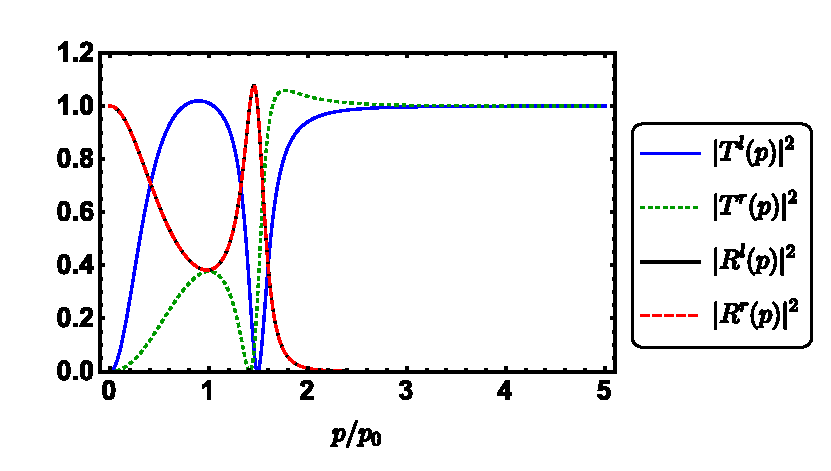
\includegraphics[width=0.75\linewidth]{Figures/VSymScattAmplitudes.eps}
\end{center}
\caption{Transmission and reflection coefficients of the time-reversal symmetric potential (symmetry V) \eqref{TRpot} with $a=p_0$, $b= 0.5\, p_0$ and $V_0>0$.}
\label{fig:VSymScattAmplitudes}
\end{figure}
%%%%%%%%%%%%%%%%%%%%%%%%%%%%%%%%%%%%%%%%%%

%
\subsection{Parity pseudohermitian potential}
%
%
As a second example we will consider  a separable potential which only fulfils symmetry IV. The normalised vector $\ket{\chi}$ in position and momentum representation is
%
\begin{eqnarray}
\braket{x}{\chi}=& \sqrt{\frac{a}{\hbar}} \begin{cases}
e^{-(a+ib)x/\hbar}  &x>0,\\ e^{a x/\hbar} &x<0,
\end{cases} \nonumber \\
\braket{p}{\chi}=&  \sqrt{\frac{a}{2\pi}} \frac{2 a+ i b}{(p+ia)(p+b-i a)},
\end{eqnarray}
%
where $a>0$ and $b$ is real.
We choose $\ket{\phi}$ as
%
\begin{eqnarray}
\braket{x}{\phi}=& \sqrt{\frac{a}{\hbar}} \begin{cases}
e^{-a x/\hbar} &x>0,\\ e^{(a+i b)x/\hbar} &x<0,
\end{cases} \nonumber \\
\braket{p}{\phi}=& \sqrt{\frac{a}{2\pi}} \frac{2 a+i b}{(p-ia)(p-b+i a)},
\end{eqnarray}
%
where $\hbar/a$ gives as before the width in coordinate representation. The potential functions in coordinate representation become asymmetrical
because of the  imaginary terms  $ib$ in  the exponent added only on  one side. This term leads to oscillations in real and imaginary parts. In momentum representation $b$ appears as a real shift in the position of one of the poles.
%
In coordinate representation the potential is
%
\begin{eqnarray}
\hspace*{-0.6cm}\la x|V|y\ra=  \frac{aV_{0}}{\hbar} \begin{cases}
e^{-\left[a (x+y) - i b y\right]/\hbar} \, ,&x>0,\,y>0\\
e^{a(y-x)/\hbar} \,  ,&x>0, \,y<0\\
e^{\left[a(x-y)+i b(x+y)\right]/\hbar} \,  ,&x<0,\,y>0\\
e^{\left[a(x+y)+i b x\right]/\hbar} \,  ,&x<0,\,y<0
\end{cases}.
\label{Ppot}
\end{eqnarray}
%
%see Fig. \ref{fig:IVSymPotentialPlot}.
The case $b=0$ implies that the potential is real and hence satisfies time-reversal symmetry (V) with equal reflection amplitudes (as in the previous case), and also symmetry VIII.


\begin{figure}[h]
\centering
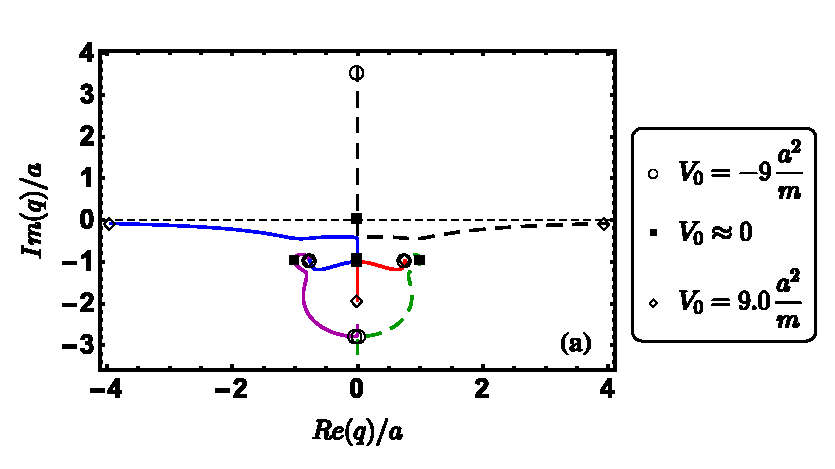
\includegraphics[width=0.75\linewidth]{Figures/IVSymEigenvalsVaryingV0new.eps}
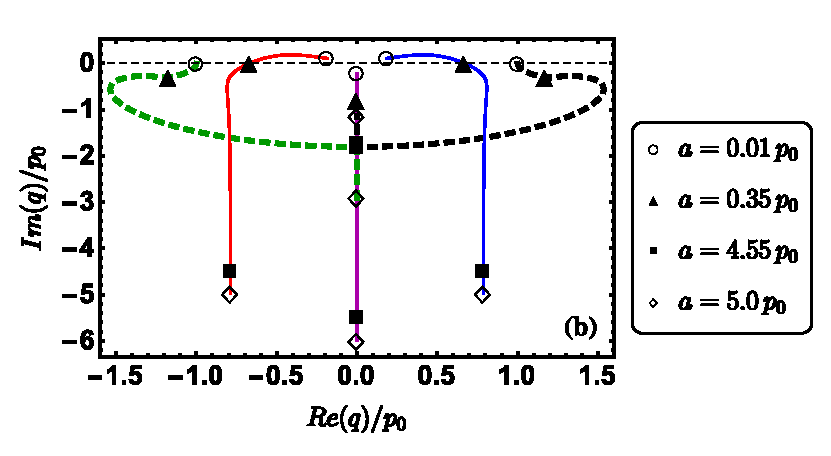
\includegraphics[width=0.75\linewidth]{Figures/IVSymEigenvalsVaryinganew.eps}
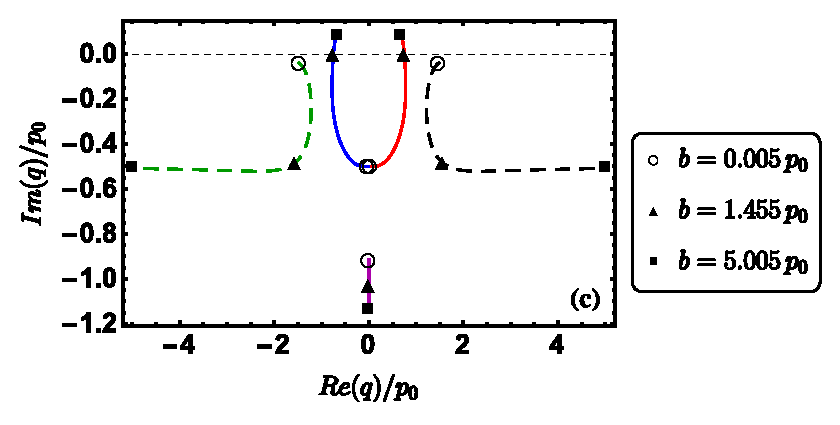
\includegraphics[width=0.75\linewidth]{Figures/IVSymEigenvalsVaryingbnew.eps}
\caption{ Poles and pole trajectories for the parity pseudohermitian potential \eqref{Ppot} (a) varying $V_0$ with $a=b$; (b) varying $a$ with $b=p_0$, $V_0>0$; (c) varying $b$ with $a=0.5\, p_0$, $V_0>0$.}
\label{fig:IVSymEigenvals}
\end{figure}



By calculating $Q_{0}$ again explicitly using complex contour integration around the poles at $-q$, $-b-i a$ and $b-i a$, we get that
%
\begin{eqnarray}
&&Q_{0}(q)/m
\nonumber\\
&&=\frac{8 a^2 q^3-4 a^2 q \left(10 a^2+b^2\right)-i a \left(4 a^2+b^2\right)^2+32 i a^3 q^2}{q \left(4 a^2+b^2\right) (a-i q)^2 \left[b^2+(a-i q)^2\right]}.
\nonumber\\
\end{eqnarray}
%
Equation \eqref{eq:chapter2_roots} has five roots in this case constituting core poles of the $S$ matrix elements.

Figure \ref{fig:IVSymEigenvals} depicts the trajectories of these poles for varying $a$, $b$ or $V_0$. As for the previous potential, the poles are symmetric with respect to the imaginary axis. In Fig. \ref{fig:IVSymEigenvals}(a) there is a single bound state for $V_0<0$ while for positive values there are a resonance/antiresonance pair and a pair of virtual states. There are collisions of eigenvalues for values of $V_0$ close to 0. In Fig. \ref{fig:IVSymEigenvals}(b)  two complex-conjugate (bound) eigenvalues cross the real axis and become a resonance/antiresonance pair. At the exact point where the eigenvalues are on the real axis, the scattering amplitudes diverge, however the eigenvalues of the $S$ matrix do not, since divergences of the left and right amplitudes cancel each other. For $a  \approx 4.55$ $p_0$ a resonance/antiresonance pair collides and becomes a pair of virtual states. In Fig. \ref{fig:IVSymEigenvals}(c) another crossing of the real axis takes place, but in this case when decreasing $b$.

Figure \ref{fig:T_R_fig2} depicts the associated transmission and reflection coefficients as functions of the momentum $p$. The eigenvalues are not always equal since parity pseudohermicity does not imply any strict restriction to them \cite{Ruschhaupt2017}. For large  momenta, i.e. $p \gg \sqrt{2} p_0$, the potential is transparent giving $T^l,T^r \approx 1$. For $p\approx 1.5$ $p_0$ the right incidence transmission has a pronounced peak. Comparing with \ref{fig:IVSymEigenvals}(c), we notice that the values of the potential parameters and the momentum are close to the ones for which the real axis crossing takes place. Around $p = 0.6$ $p_0$ the potential acts as a $\mathcal{T}/\mathcal{R}$ device or one-way-barrier (see table \ref{tab:chapter1_DevicesDescription}).


\begin{figure}[t]
\begin{center}
  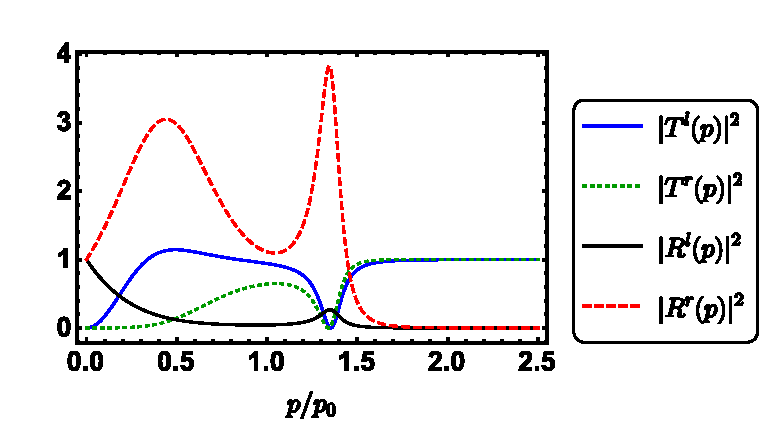
\includegraphics[width=0.75\linewidth]{Figures/IVSymTR.eps}
\end{center}
\caption{ Transmission and reflection coefficients for $a=b=0.5\, p_0$ and $V_0>0$.}
\label{fig:T_R_fig2}
\end{figure}


\section{Discussion}
\label{sec:chapter2_Discussion}

In this chapter I have studied some aspects of the scattering of a structureless particle in one dimension by
generally non-local and non-Hermitian potentials.

Conditions that were found for discrete Hamiltonians to imply conjugate pairs of discrete eigenenergies
(pseudohermiticity with respect to a linear operator or commutativity of $H$ with an antilinear operator \cite{Mostafazadeh2002,Mostafazadeh2002a,Mostafazadeh2002b}) can in fact be extended to scattering Hamiltonians in the continuum, implying symmetry relations not just for bound-state eigenvalues
but also for complex
poles of the $S$-matrix. Specifically the poles of $S$ matrix eigenvalues
are symmetrically located with respect to the imaginary axis, also in the lower momentum plane, so that resonances and antiresonance
energies are conjugate pairs as well.
In  terms of the eight possible Hamiltonian symmetries associated with Klein's group of $A$ operators (unity, parity, time reversal and PT)
and their commutation or pseudohermiticity with $H$,
the symmetrical disposition of the poles applies to four of them, which includes hermiticity and PT-symmetry. Potential models
and pole motions are provided for the
two other non trivial symmetries: time-reversal symmetry and parity pseudohermiticity.

The study contributes to deepen our understanding of asymmetric scattering  (with different responses for left/right incidence) beyond the
% much studied  PT-symmetric potentials. This work opens interesting perspectives in AMO physics where much activity on asymmetric-scattering, mostly via optical devices,   is currently being carried out.
    % Symmetries of non-Hermitian potentials S-matrix poles
%!TEX root = ../Thesis.tex
%Chapter 3

\chapter{Quantum-Optical implementation of non-Hermitian potentials for asymmetric scattering}
\label{Chapter3}
\lhead{Chapter 3. \emph{Quantum-Optical implementation of non-Hermitian potentials for asymmetric scattering}}

In chapters \ref{Chapter1} and \ref{Chapter2}, non-local potentials for asymmetric scattering were constructed as mathematical models but no physical implementation was discussed. In this chapter a feasible quantum-optical implementation
of non-Hermitian, non-local, non-PT potentials is put forward to implement different scattering asymmetries, including transmission
asymmetries. Using Feshbach's projection technique it is found that the effective potentials for a ground-state atom crossing a laser beam in a region of space are generically non-local and non-Hermitian. Shaping the spatial-dependence of the, generally complex, Rabi frequency, and selecting a specific laser detuning allows to produce different potential symmetries and asymmetric scattering effects, including asymmetric transmission.

The rest of this chapter is organized as follows. In section \ref{sec:chapter3_enl}, I shall explain how to generate different non-Hermitian symmetries in a quantum-optical setting of an atom impinging on a laser illuminated region. In section \ref{sec:chapter3_exa}, I provide specific examples of devices (constructed using numerical optimisation) with different asymmetric scattering responses. Realistic experimental parameters are also examined. In section \ref{sec:chapter3_class}, the asymmetric behavior is explained with a classical approximation of the motion and the non-commutativity of rotations on the Bloch sphere, which gives good estimates for the potential parameters. Finally, in section \ref{sec:chapter3_Discussion}, I summarize the main findings in the chapter.

%---------------------------------------------------------------------------------------------
\begin{table}[t]
  \caption{Conditions leading to  specific symmetries in the potential \eqref{eq:chapter3_effpot}. A given symmetry also implies others, see the last column.\label{tab:chapter3_SymmetriesConditions}}
  \hspace*{-0.1cm}
  \centering
  \begin{tabular}{lcc}
  \hline\hline
  Symmetry& Conditions & Implies
  \\
  \hline
  (I)\;$1H=H1$ &   none & -
  \\
  (II)\;$1H=H^\dagger 1$ &  $q=-q^{*}$ (i.e. $\operatorname{Re}q=0$) & I
  \\
  (III)\;$ \Pi H=H\Pi$ &  $\Omega(x)=e^{i\phi}\Omega(-x)$ & I
  \\
  (IV) $\Pi H=H^\dagger \Pi$ &  $q=-q^{*}$ \& $\Omega(x)=e^{i\phi}\Omega(-x)$ & III,\! II,\! I
  \\
  (V) $\Theta H=H\Theta$ &  $q=-q^{*}$ \& $\Omega(x)=e^{i\phi}\Omega(x)^*$ & {\small VI,\! II,\! I}
  \\
  (VI) $\Theta H=H^\dagger\Theta$ &  $\Omega(x)=e^{i\phi}\Omega(x)^*$ & I
  \\
  (VII) $\Theta\Pi H=H\Theta \Pi$ &  $q=-q^{*}$ \& $\Omega(x)=e^{i\phi}\Omega(-x)^*$ & VIII,\! II,\! I
  \\
  (VIII)\,$\Theta\Pi H=H^\dagger \Theta \Pi$ &  $\Omega(x)=e^{i\phi}\Omega(-x)^*$  & I
  \\
  \hline\hline
  \end{tabular}
\end{table}
%---------------------------------------------------------------------------------------------

%
\section{Effective non-local potential for the ground state of a two-level atom\label{sec:chapter3_enl}}
%
The key task is to physically realize some of the potential and asymmetric device types described in chapter \ref{Chapter1}, which are again summarized in table \ref{tab:chapter3_table2PhysicalImplementation}. I start with a two-level atom with ground level $\ket{1}$ and excited state $\ket{2}$ impinging onto a laser illuminated region. For a full account of the model and further references see
\cite{Ruschhaupt2009}. The motion is assumed to be one dimensional, either because the atom is confined in a waveguide or because the direction $x$ is uncoupled to
the others.
I only account explicitly for atoms before the first spontaneous emission in the wave function
\cite{Hegerfeldt1996,Damborenea2002,Navarro2003}.
If the excited atom emits a photon, it disappears from the coherent wave function ensemble.
I assume that no resetting into the ground state occurs. The physical mechanism
may be an irreversible decay into a third level  \cite{Oberthaler1996}, or atom ejection from the waveguide or the privileged 1D direction due to  random recoil  \cite{Streed2006}.
The state ${\bf\Phi}_k=\left(\begin{smallmatrix}\phi_k^{(1)},\phi_k^{(2)}\end{smallmatrix}\right)^{\sf T}$
for the atom before the first spontaneous emission impinging with wave number $k$
in a laser adapted  interaction picture,
obeys, after applying the rotating-wave approximation, an effective stationary Schr\"{o}dinger equation
with a time-independent Hamiltonian \cite{Ruschhaupt2004a,Ruschhaupt2009}
%
${\cal H}{\bf\Phi}_k(x)=E{\bf\Phi}_k(x)$,
%
where
%
\begin{eqnarray}
  {\cal H}&=& H_0{\bf 1}+ {\cal V}=\frac{1}{2m}\left(
  {{p}^2\atop 0}{0\atop {p}^2}\right)+ {\cal V}(x),
  \\
  {\cal V}(x) &=&
  \frac{\hbar}{2}\left(
  {0\atop \Omega(x)^*}\;\;\;\;
  {\Omega(x)\atop -(2\Delta+i\gamma)}
  \right).
\end{eqnarray}
%
I assume perpendicular incidence of the atom on the laser beam for simplicity. Here $E=\hbar^2 k^2/2m$ is the energy, and
$\Omega(x)$ is the position-dependent, on-resonance Rabi frequency, where real and imaginary parts may be controlled independently
using two  laser field quadratures  \cite{Zhang2013};
$\gamma$ is the inverse of the lifetime of the excited state;
$\Delta=\omega_{L}-\omega_{12}$
is the detuning (laser angular frequency minus the atomic transition
angular frequency $\omega_{12}$);
${p}=-i\hbar\partial/\partial x$ is the momentum operator;
and ${\bf 1}=|1\ra\la 1|+|2\ra\la 2|$ is the unit operator
for the internal-state space.
Complementary projectors
%
$P=|1\ra\la 1|$ and $Q=|2\ra\la 2|$
%
are defined to select ground and excited state components.
Using the Feshbach partitioning
technique \cite{Feshbach1958,Feshbach1962,Levine1969},
I find for the ground
state amplitude $\phi_k^{(1)}$ the equation
%
\begin{equation}\label{effecti}
  E\phi_k^{(1)}(x) = H_0\phi_k^{(1)}(x)+\!
  \int\! dy\, \la x,1|{\cal W}(E)|y,1\ra \phi_k^{(1)}(y),
\end{equation}
%
where
%
$
{\cal W}(E)=P{\cal V}P+P{\cal V}Q(E+i0-Q{\cal H}Q)^{-1}Q{\cal V}P,
$
%
is generically non-local and energy-dependent. Specifically, I have now achieved
a physical realization of an effective (in general) non-local, non-Hermitian potential whose kernel has the form
%
\begin{eqnarray}
  \hspace*{-.3cm}V (x,y) = \la x,1|{\cal W}(E)|y,1\ra = \frac{m}{4} \frac{e^{i|x-y|q}}{i q}
  \Omega(x)\Omega(y)^*,
  \label{eq:chapter3_effpot}
\end{eqnarray}
%
%
where
$
q=\frac{\sqrt{2mE}}{\hbar}(1+\mu)^{1/2},\;\;
{\rm Im}\,q\ge 0,
\label{qeq}
$ and
$
\mu=\frac{2\Delta+i\gamma}{2E/\hbar}.
$
%
eq. \eqref{eq:chapter3_effpot} is worked out  in momentum representation to do the integral
using the residue theorem.
This is a generalized, non-local version of the effective potentials known for the ground state
\cite{Chudesnikov1991,Oberthaler1996}, which are found from eq. \eqref{eq:chapter3_effpot}  in the large $\mu$ limit \cite{Ruschhaupt2004a}.
The reflection and transmission amplitudes $R^{r,l}$ and  $T^{r,l}$ may be calculated directly
using the potential \eqref{eq:chapter3_effpot} or as corresponding amplitudes for
transitions from ground state to ground state in the full two-level theory (see Appendix \ref{Appendix:NumericalCalculationOfTandR}).

%%%%%%%%%
\begin{table}
  \caption{Device types for  transmission and/or reflection asymmetry in the first row (see section \ref{sec:chapter1_AsymmetricDevices} for nomenclature).
  The second row gives the corresponding symmetries  that allow
  each device.
  \label{devices}}
  \vspace*{.0cm}
  \label{tab:chapter3_table2PhysicalImplementation}
  \centering
  \begin{tabular}{cccccc}
    \hline\hline
    $\cal{TR/A}$ & $\cal{T/R}$ & $\cal{T/A}$ & $\cal{TR/R}$ & $\cal{R/A}$ & $\cal{TR/T}$ \\
    \hline
    I            & I           & I,VIII      & I,VIII       & I,VI        & I, IV, VI, VII
    \\
    \hline\hline
  \end{tabular}
\end{table}
%

\subsection{Possible symmetries of the non-local potential}
%
The necessary conditions for the different symmetries of a non-Hermitian and non-local Hamiltonian were worked out in section \ref{sec:chapter1_AsymmetricDevices}. In the second column of table \ref{tab:chapter3_SymmetriesConditions}, those conditions have been particularized for the effective potential of the 2-level atom \eqref{eq:chapter3_effpot}. For example, symmetry III (parity) requires that $V(x,y)=V(-x,-y)$ (see table \ref{tab:chapter1_SymmetriesTable}). Inserting the functional form of the potential from eq. \eqref{eq:chapter3_effpot} into this condition, it results in the requirement $\Omega(x) \Omega(y)^* = \Omega(-x) \Omega(-y)^*$. This is fulfilled if $\Omega(x)=\Omega(-x)e^{i \phi}$ with some arbitrary phase freedom $\phi$.

Since $\Omega(x)$ does not depend on $q$, symmetries IV, V and VII imply that symmetry II is obeyed as well (Hermiticity).
Moreover, symmetry III (parity) should be discarded for our purpose since it does not allow for asymmetric transmission or reflection
\cite{Ruschhaupt2017}.
This leaves us with three interesting symmetries to explore:
VI, which allows for  asymmetric reflection; VIII which allows for asymmetric transmission; and  I,
which in principle allows for arbitrary asymmetric responses, except for physical limitations imposed by
the two-level model see Appendix \ref{Appendix:NumericalCalculationOfTandR}.

As seen from  table \ref{tab:chapter3_SymmetriesConditions}, $\operatorname{Re}(q)=0$ makes the potential Hermitian, so it must be avoided.
If $\gamma=0$,   $\mu \in \mathbb{R}$. Hence $\mu+1<0$ gives $\operatorname{Re}(q)=0$ and $\mu+1>0$ gives
$\operatorname{Im}(q)=0$. $\mu+1>0$ amounts to a condition on the detuning compared to the incident energy, namely $\Delta>-E/\hbar$.
In the following I implement potentials with symmetries VIII, VI, and I, with detunings and energies satisfying the condition $\mu+1>0$.


\section{Design of asymmetric devices\label{sec:chapter3_exa}}

I will now apply this method to physically realize non-local potentials of the form \eqref{eq:chapter3_effpot}. I shall work out explicitly a ${\cal T/A}$ device with symmetry  VIII, an ${\cal R/A}$ device with symmetry  VI, and a ``partial''-${\cal TR/A}$ device,  having 1/2 transmission and reflection coefficients from the left, with symmetry I. The  ${\cal T/A}$ and the ``partial''-${\cal TR/A}$ device have transmission asymmetry so they cannot be built with local or $PT$-symmetric  potentials.
%, whereas   to design asymmetric devices which can be shown not to be implementable with a one-dimensional, one-channel, local potential.
Let us  motivate the effort with some possible applications, relations  and analogies of these devices.
${\cal T/A}$ and ${\cal R/A}$ are, respectively, transmission and reflection filters. They are analogous to
half-wave electrical rectifiers that either let the signal from one side ``pass'' (transmitted) or change its sign (reflected)
while suppressing the other half signal.  They may play the role of half-rectifiers in atomtronic circuits.
A ${\cal T/A}$ device allows us, for example, to empty a region of selected particles, letting them go away while not letting particles in.
The ``atom diode'' devices worked out e.g. in \cite{Ruschhaupt2004,Ruschhaupt2006a,Ruschhaupt2006,Ruschhaupt2007}
were of type ${\cal R/A}$. As the mechanism behind them was adiabatic, a broad range of momenta with the desired asymmetry
could be achieved. In comparison, the current approach is not necessarily adiabatic so it can be adapted to faster processes.

As for the ``partial''-${\cal RT/A}$ device,  it reflects and transmits from one side while absorbing from the
other side. In an optical analogy an observer from the left perceives it as a darkish mirror.
An observer from the right ``sees'' the other side because of the allowed transmission
but cannot be seen from the left since  nothing is transmitted from right to left. Our device is necessarily a ``partial'' one as
there cannot be  net probability gain because of the underlying two-level system, and a ``full'' version with both reflection and transmission coefficients equal to one
would need net probability gain.

The three devices are worked out for $\gamma=0$, a valid approximation for  hyperfine transitions. %, although this is by no means a necessary assumption.
I assume for the Rabi frequencies the forms
%
\begin{eqnarray}
  \Omega_{\rm VIII} (x) &=& a [g(x+x_0) + i  g(x-x_0)],
  \nonumber\\
  \Omega_{\rm VI} (x) &=&  b g(x+x_0) + c g(x-x_0),
  \nonumber\\
  \Omega_{\rm I} (x) &=&  - i b g(x+x_0) + c g(x-x_0),
  \label{3omegas}
\end{eqnarray}
%
in terms of smooth, realizable Gaussians $g(x) =  \exp[-{x^2}/{w^2}]$.
I fix $2 d$ as an effective finite width
of the potential area beyond which the potential is negligible and assumed to vanish. I will express in the following the different length parameters as a multiple of $d$ to keep results general.
In addition, I will use as a scaling factor for the velocity $v_{d} = {\hbar}/({m d})$, and for time $\tau={m d^2}/{\hbar}$.

In the following calculations I fix the width of the Gaussians to be $w= {\sqrt{2}}d/{10}$.
I always first set a target velocity $v_0$ to achieve the desired asymmetric scattering response.
The real parameters $a$, $b$, $c$, $x_0$ in eq. \eqref{3omegas}, and  $\Delta$
are then numerically optimized with the GRAPE (Gradient Ascent Pulse Engineering) algorithm \cite{Khaneja2005,Wu2015}.

The Rabi frequencies will fulfill the indicated symmetries VIII, VI, and I. $\Omega_{\rm VI}(x)$ should not be even (i.e. $b \neq c$) to avoid symmetry II. In addition, $\Omega_{\rm I}(x)$ should not fulfill any other symmetry than ${\rm I}$.
The corresponding Rabi frequencies $\Omega(x)$ are  depicted in figs. \ref{fig_t_a}, top row.
The scattering coefficients are shown in the bottom row. fig. \ref{fig_t_a} demonstrates that the three potentials satisfy the asymmetric response conditions imposed
at the selected velocity and also in a region nearby.

The ``partial''-${\cal TR/A}$  device fullfills $\absq{T^l} = \absq{R^l} = 1/2$ and full absorption from the right.
The potential I use for that device has symmetry I only, i.e., ``no symmetry'' other than the trivial commutation with the identity. No other potential symmetry would allow this type of device.

The effective non-local potential $V(x,y)$, see eq. \eqref{eq:chapter3_effpot}, corresponding to the $v/v_d$ ratios used for the three devices is shown in fig. \ref{fig_poten1}. Note that the non-local potential has dimensions  energy/length, so  we
divide the absolute value by a factor $V_0=\hbar^2/(m d^3)$ to plot a dimensionless quantity.


% -------------------------------------------------------------
\begin{figure}
  \begin{center}
  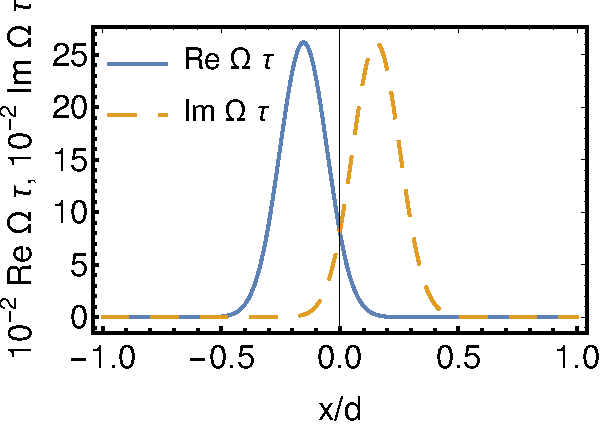
\includegraphics[width=0.28\linewidth]{Figures/asym_fig_t_a_400_pot.pdf}
  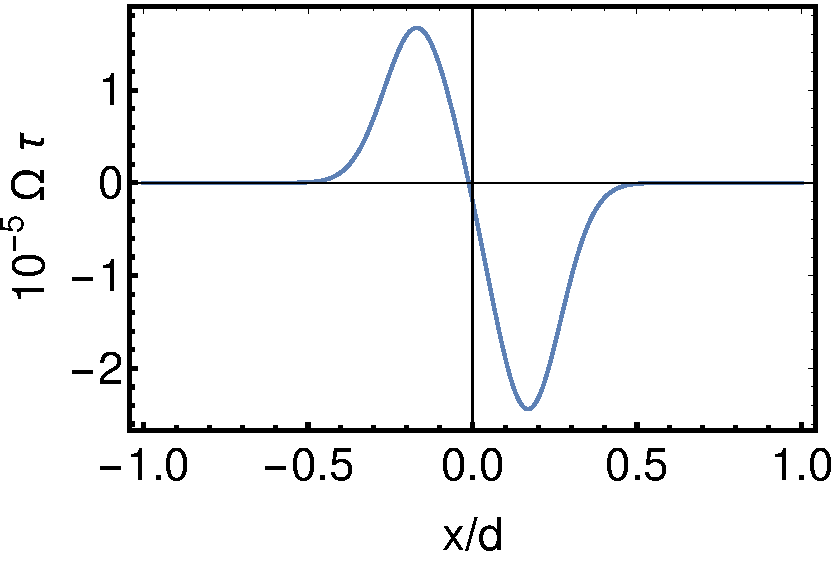
\includegraphics[width=0.28\linewidth]{Figures/asym_fig_r_a_400_pot.pdf}
  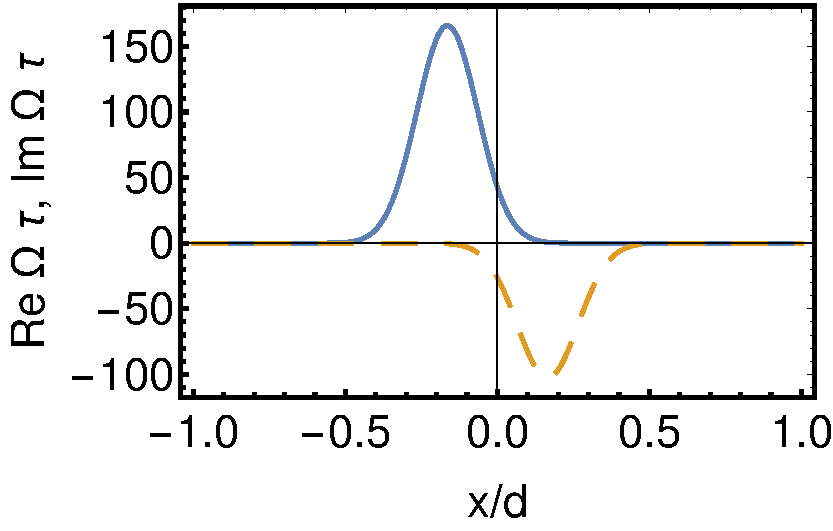
\includegraphics[width=0.28\linewidth]{Figures/asym_fig_1_2_tr_a_8_pot.pdf}\\
  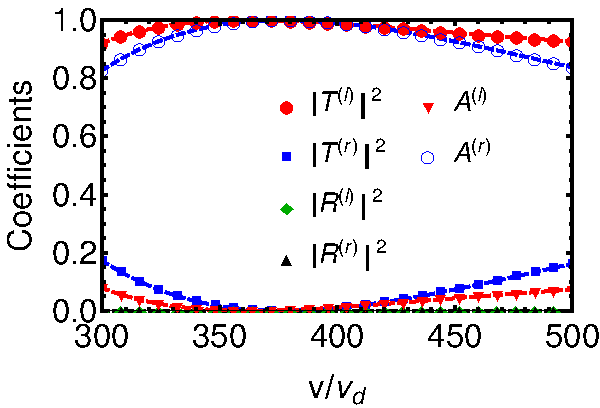
\includegraphics[width=0.29\linewidth]{Figures/asym_fig_t_a_400.pdf}
  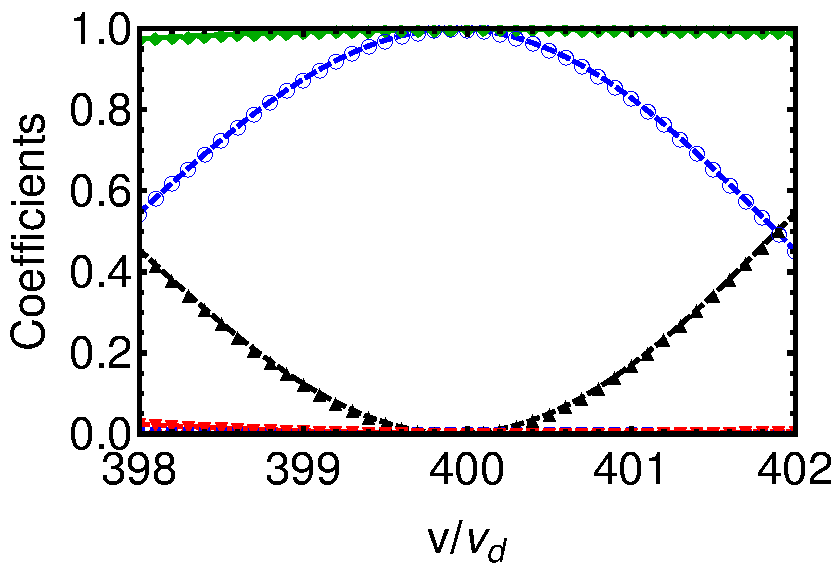
\includegraphics[width=0.29\linewidth]{Figures/asym_fig_r_a_400.pdf}
  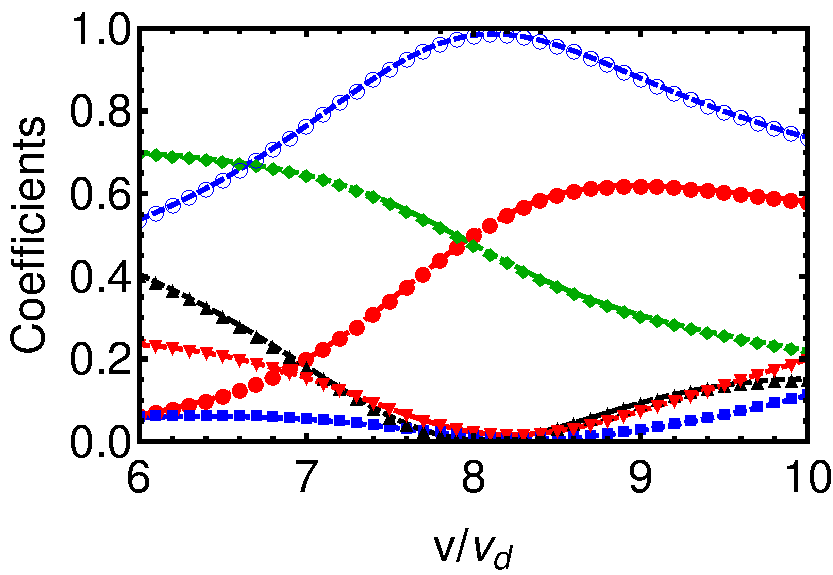
\includegraphics[width=0.29\linewidth]{Figures/asym_fig_1_2_tr_a_8.pdf}
  \end{center}
  \caption{Left column: ${\cal T/A}$ device with symmetry VIII.
  Top: $\Omega_{\rm VIII}(x)$;
  Bottom:  transmission and reflection coefficients. $v_0/v_d=400$, $a\tau = 2618.19$,
  $x_0/d = 0.1532$, $\tau\Delta = 1413.01$.
  %
  Middle column: ${\cal R/A}$ device with symmetry VI.
  Top: $\Omega_{\rm VI} (x)$ (it is real); Bottom:  transmission and reflection coefficients. $v_0/v_d=400$,
  $b \tau =  -244516.1$,
  $c\tau = 167853.9$,
  $x_0/d = 0.1679$,
  $\tau\Delta= 193.508$.
  %
  Right column: ``Partial''-${\cal TR/A}$ device with symmetry I.
  Top:  $\Omega_{\rm I}(x)$, real (blue, solid line) and imaginary parts (orange, dashed line);
  Bottom: transmission and reflection coefficients. $v_0/v_d=8$, $b\tau =  102.6520$,
  $c \tau =  165.8355$,
  $x_0/d = 0.1648$,
  $\tau\Delta= 90.5337$. In all cases $\tau={m d^2}/{\hbar}$ and $v_{d} = {\hbar}/({m d})$.
  \label{fig_t_a}}
\end{figure}
% -------------------------------------------------------------

%--------------------------------------------------------------------------
\begin{figure}
  \begin{center}
  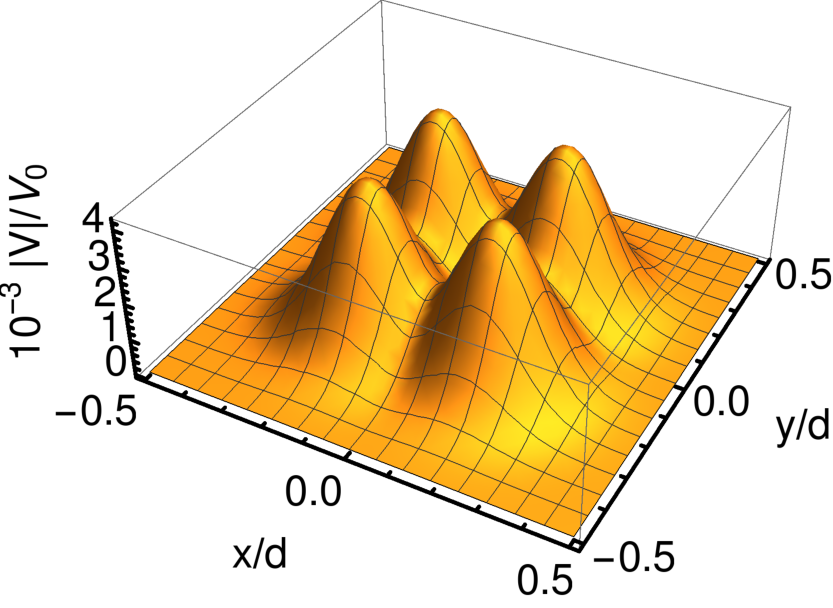
\includegraphics[width=0.28\linewidth]{Figures/asym_fig_t_a_400_eff_pot_abs.pdf}
  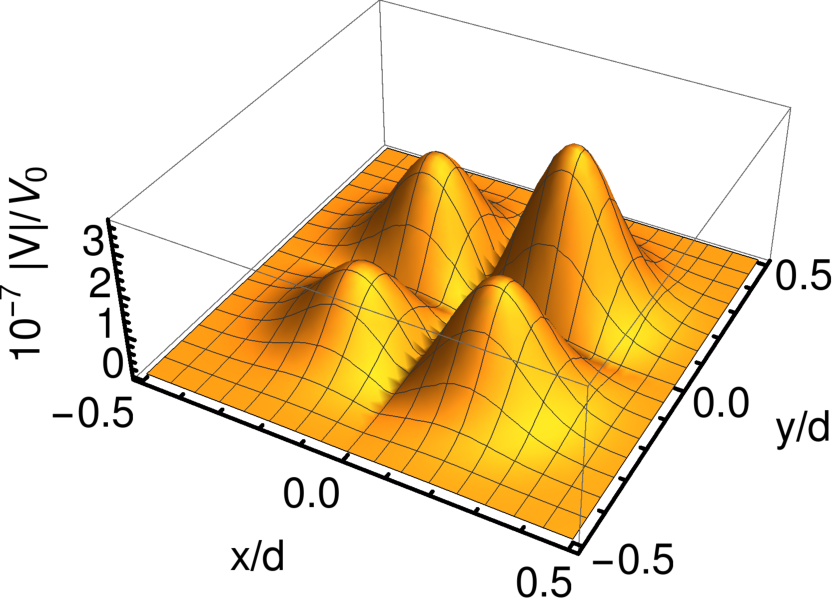
\includegraphics[width=0.28\linewidth]{Figures/asym_fig_r_a_400_eff_pot_abs.pdf}
  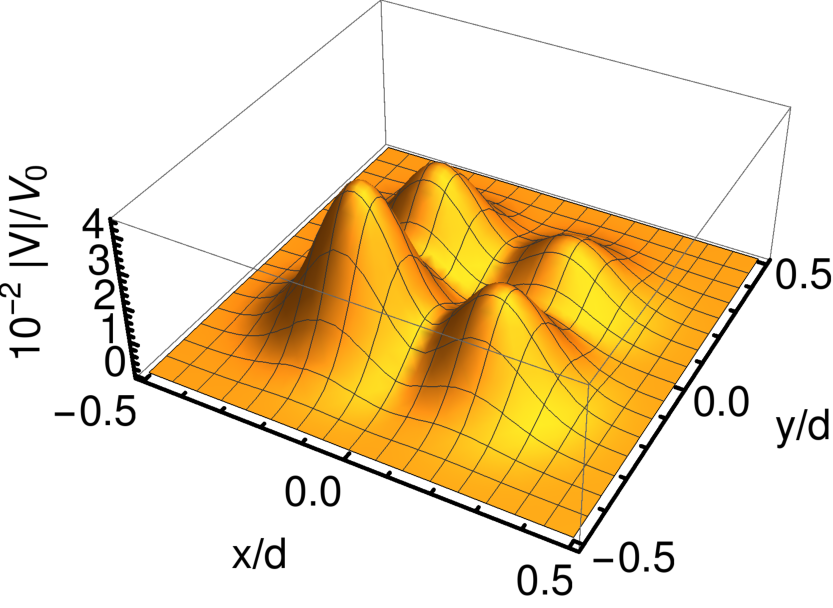
\includegraphics[width=0.28\linewidth]{Figures/asym_fig_1_2_tr_a_8_eff_pot_abs.pdf}\\
  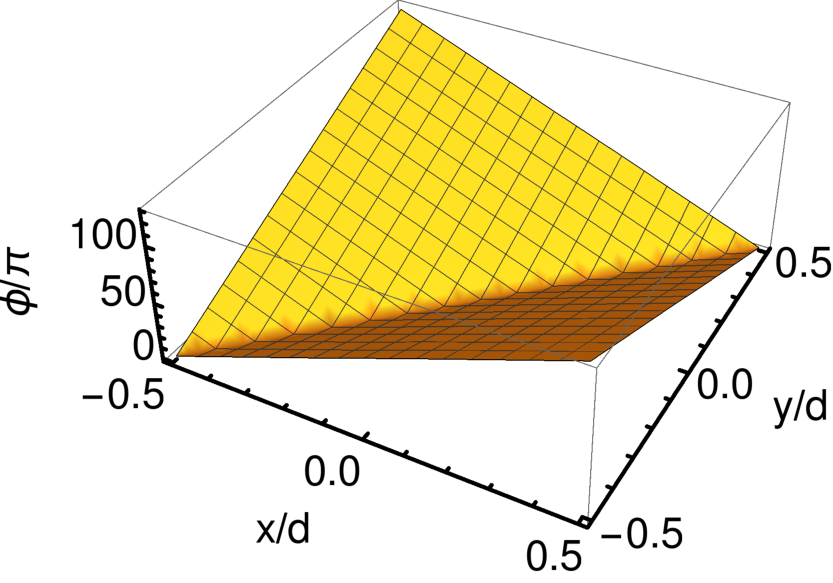
\includegraphics[width=0.29\linewidth]{Figures/asym_fig_t_a_400_eff_pot_arg.pdf}
  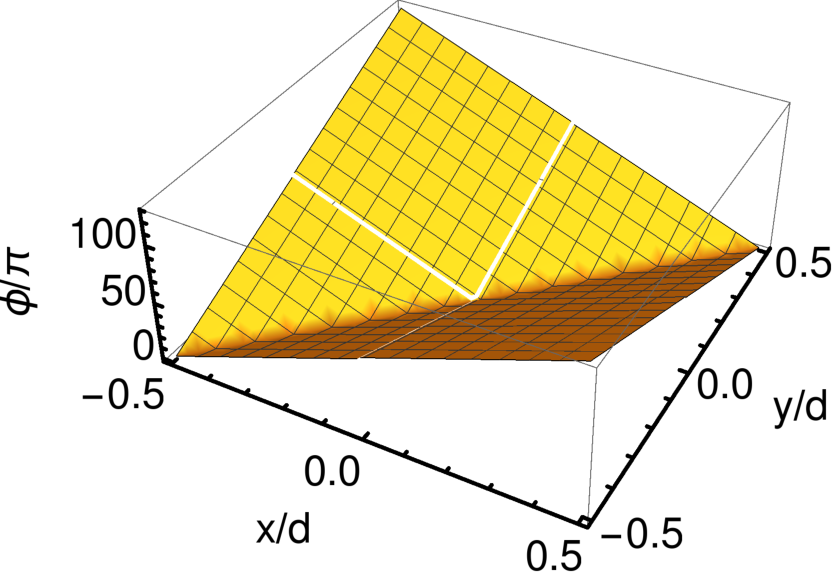
\includegraphics[width=0.29\linewidth]{Figures/asym_fig_r_a_400_eff_pot_arg.pdf}
  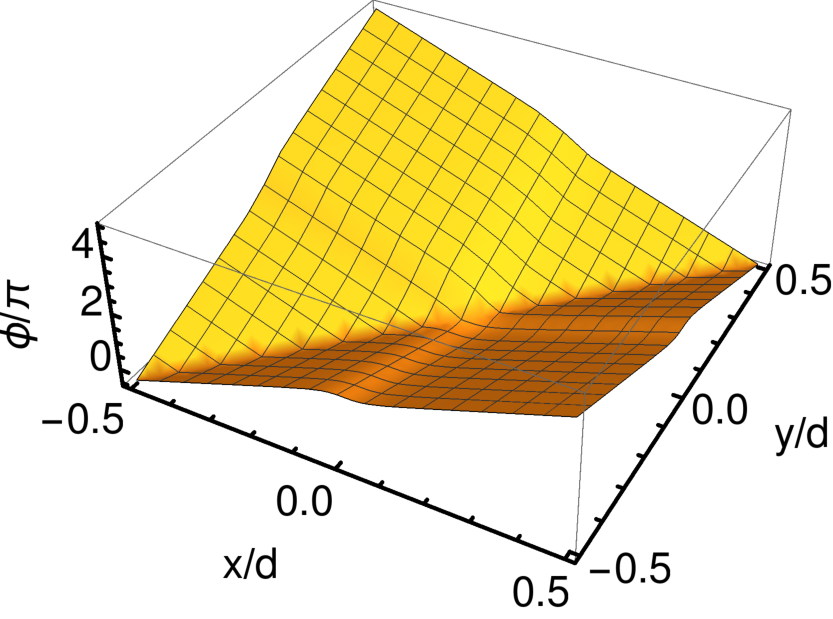
\includegraphics[width=0.29\linewidth]{Figures/asym_fig_1_2_tr_a_8_eff_pot_arg.pdf}
  \end{center}
  \caption{Non-local potentials  $V(x,y)$: absolute value (top), argument (bottom).
  Left column: Potential for ${\cal T/A}$ device with symmetry VIII.
  Middle column: Potential for ${\cal R/A}$ device with symmetry VI.
  Right column: ``Partial''-${\cal TR/A}$ device with symmetry I.
  $V_0=\hbar^2/(md^3)$.}
  \label{fig_poten1}
\end{figure}
%--------------------------------------------------------------------------

In the parameter optimization I see that increasing the velocities further does not pose a problem for the ${\cal T/A}$
device, it is more challenging for an ${\cal R/A}$ device, and it is quite difficult for the partial-${\cal RT/A}$ device.  The device ${\cal T/A}$ is feasible for an experimental implementation  as the ratio $v_0/v_d$ can be easily increased to desired values, for  reasonable values of the
Rabi frequency and laser waist \cite{Zeyen2016}.

Moreover, the velocity width with the desired behavior is much broader for ${\cal T/A}$. Therefore a ${\cal T/A}$
device is the best candidate for
an experimental implementation.
As a check of feasibility, let us assume a Beryllium ion. Its hyperfine structure provides a good  two-level system
for which I can neglect decay (i.e. $\gamma\approx 0$ is indeed realistic). $m=1.49\times 10^{-26}$ kg
and I set a length $d=10\, \mu$m compatible with the small laser waists (in this case 1.4 $\mu$m) achieved for individual ion
addressing \cite{Zeyen2016}. The scaling factors take the values
%
\begin{eqnarray}
  v_d&=&0.67\, {\rm mm/s},
  \nonumber\\
  \tau&=&1.49\times 10^{-2}\, {\rm s},
  \nonumber
\end{eqnarray}
%
which gives  $v\approx$ 27 cm/s for $v/v_d=400$, (there is no major obstacle to get devices for higher velocities,
in particular the classical approximations in section \ref{sec:chapter3_class} can be used to  estimate the values of the parameters)
and Rabi frequencies, see fig. \ref{fig_t_a},  in the hundreds of kHz range. The relative ion-laser beam velocity could be as well
implemented  by moving the beam in the laboratory frame.

%
%
\section{Classical approximation for ${\cal T/A}$ device \label{sec:chapter3_class}}
%
%
In a ${\cal T/A}$ device such as the one presented, an incident plane wave from the left ends up as a pure transmitted wave with no reflection or absorption.
However, a wave incident from the right is fully absorbed. How can that be? Should not the velocity-reversed motion
of the transmitted wave lead to the reversed incident wave?
%Obviously that is not the case, and a formal answer to that question  is that $V$ is not time-reversal invariant.
For a more intuitive understanding I may seek help in the underlying two-level model.
In the larger space the potential is again local and Hermitian. A simple semiclassical
approximation is to assume that the particle moves with  constant speeds $\pm v$ for left ($v>0$) or right ($-v<0$) incidence,  so that at a given time it is subjected to  the $2\times2$ time-dependent potentials
${\cal V}(\pm vt)$. The incidence from the left and right give different time dependences for the potential. The scattering problem then reduces to solving the time-dependent Schr\"odinger equation for the amplitudes of a two-level atom with time-dependent potential, i.e. to solving the following time-dependent Schr\"odinger equation ($\gamma = 0$)
%
\begin{eqnarray}
  i \hbar \frac{\partial}{\partial t} \chi_\pm(t)
  = {\cal V} (\pm v t) \chi_\pm(t),
\end{eqnarray}
%
with the appropriate boundary conditions $\chi_+ (-\infty) = \chi_- (-\infty) =\left(\begin{smallmatrix} 1\\ 0\end{smallmatrix}\right)$. The  solutions for $v/v_d = 400$
%9.1
are shown in fig. \ref{fig_t_a_approx}.
In fig. \ref{fig_t_a_approx}(a), $\chi_+ (t)$ (left incidence) is depicted:  the particle ends  with high probability in the ground state at the final time. In fig. \ref{fig_t_a_approx}(b), $\chi_- (t)$ (right incidence) shows that the ground state population is transferred to the excited state. Projected onto the ground-state level alone,
this corresponds to full absorption of the ground state population at the final time.

For an  even rougher but also illustrative picture,  again in a semiclassical time-dependent framework, I  may substitute the smooth Gaussians for Re$(\Omega)$ and Im$(\Omega)$ in fig. \ref{fig_t_a} by two simple, contiguous square functions of height
$\Omega>0$ and width $\tilde{w} > 0$. Then, the $2\times2$ potential at a given time is, in terms of Pauli matrices,
%
\begin{eqnarray}
  {\cal V} (x) = \frac{\hbar}{2}\Delta (\sigma_Z-{\mathbf 1})+ \frac{\hbar}{2} \left\{\begin{array}{cc}
  \Omega\sigma_X & -\tilde w < x < 0\\
  -\Omega\sigma_Y & 0 < x < \tilde w\\
  0 & \mbox{otherwise}
  \end{array}\right.
\end{eqnarray}
%
where $x = \pm v t$ and let ${\sf T}=2 \tilde w/v$.

% ------------------------------------------------------------------------------
\begin{figure}
  \begin{center}
  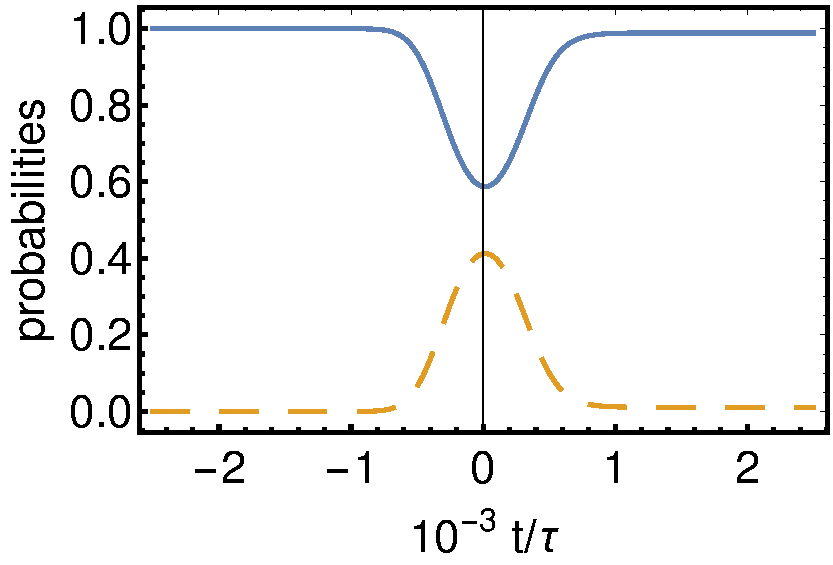
\includegraphics[width=0.48\linewidth]{Figures/asym_fig_t_a_approx_left.pdf}
  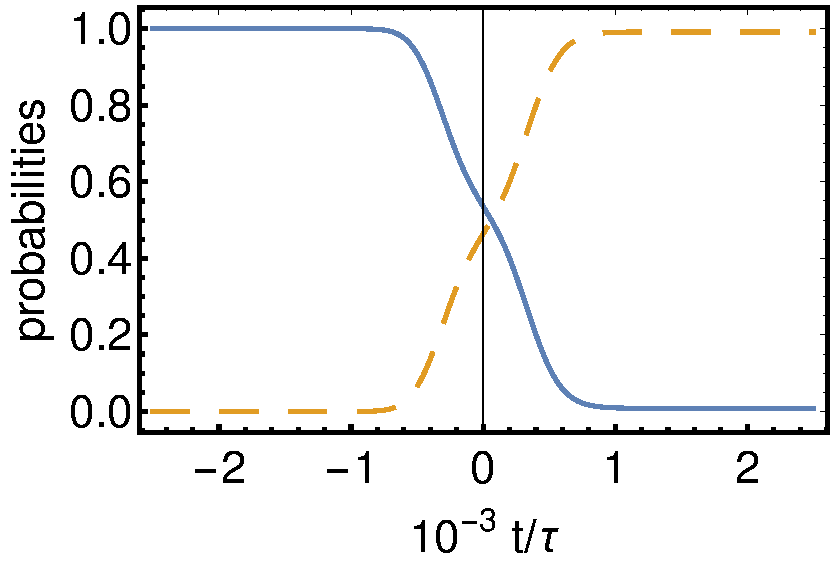
\includegraphics[width=0.48\linewidth]{Figures/asym_fig_t_a_approx_right.pdf}
  \end{center}
  \caption{Simplified model of the asymmetric ${\cal T/A}$ device with symmetry VIII: (a) $\chi_+(t)$, (b) $\chi_-(t)$; ground-state population $\absq{\chi_{\pm(t),1}}$ (blue, solid line), excited-
  $\absq{\chi_{\pm(t),2}}$ (orange, dashed line). $v/v_d = 400$, $a\tau = 2618.19$,
  $x_0/d = 0.1532$, $\tau\Delta = 1413.01$.
  \label{fig_t_a_approx}}
\end{figure}
% ------------------------------------------------------------------------------

% ------------------------------------------------------------------------------
\begin{figure}
  (a) Order of rotations:  first  $R_1({\sf T}/2)$ (left figure) and then $R_2({\sf T}/2)$ (right figure).
  \begin{center}
  % \vspace*{-0.32cm}
  \includegraphics[width=0.4\linewidth]{Figures/"asym_fig_sphere_left1"}\,\includegraphics[width=0.4\linewidth]{Figures/"asym_fig_sphere_left2"}\\[0.1cm]
  \end{center}
  (b) Order of rotations: first $R_2({\sf T}/2)$ (left figure) and then $R_1({\sf T}/2)$ (right figure).
  % \vspace*{-0.32cm}
  \begin{center}
  \includegraphics[width=0.4\linewidth]{Figures/"asym_fig_sphere_right1"}\,\includegraphics[width=0.4\linewidth]{Figures/"asym_fig_sphere_right2"}
  \end{center}
  \vspace*{-.8cm}
  \caption{Simplified time-dependent model of the asymmetric ${\cal T/A}$ device with symmetry VIII: Bloch sphere explaining non time-reversal invariance, see text for details. The state trajectories are depicted in two-steps on the sphere. The rotation axes are
  also depicted. (a) The process simulates incidence from the left. The state starts and ends in $|1\ra$. (b) The process simulates incidence from the right. The state starts at $|1\ra$ and ends at $|2\ra$.
  \label{fig_t_a_simple2}}
\end{figure}
% ------------------------------------------------------------------------------


The time-evolution of this process, $\chi_\pm (t)$,
up to a phase factor may be regarded as
two consecutive rotations $R_j=e^{-i{\beta}{\bf n}_j\cdot {\boldsymbol{\sigma}}/2}$ ($j=1,2$), with $\beta=\frac{{\sf T}}{2}\sqrt{\Omega^2+\Delta^2}$, of the two-level state on the Bloch sphere about the axes
%
\begin{eqnarray}
  {\bf n}_1&=&\frac{1}{\sqrt{\Omega^2+\Delta^2}}(\Omega,0,\Delta), %real
  \\
  {\bf n}_2&=&\frac{1}{\sqrt{\Omega^2+\Delta^2}}(0,-\Omega,\Delta). %imag
\end{eqnarray}
%
The initial state at a time $t=-{\sf T}/2$ is again $\chi_+ (-{\sf T}/2) = \chi_- (-{\sf T}/2) =\left(\begin{smallmatrix} 1\\ 0\end{smallmatrix}\right)$.
The unitary time-evolution operator to reach the final time ${\sf T}/2$ takes the form
$e^{i\Delta {\sf T}/2}R_2 R_1$ for  incidence from the left ($\chi_+$) and
$e^{i\Delta {\sf T}/2}R_1 R_2$ for incidence from the right ($\chi_-$).
The time ${\sf T}$ and the parameters $\Omega, \Delta$ will be fixed to reproduce the results of the full calculation with the exact model so that the system starts in the ground state to end either in the ground state
($\absq{\chi_{+} ({\sf T}/2)} = 1$)
or in the excited state by performing the rotations in one order or the reverse order
($\absq{\chi_{-} ({\sf T}/2)} = 0$). This gives $\Omega/\Delta = \sqrt{2}$ and ${\sf T}= 4\pi/(3 \sqrt{3} \Delta)$. It follows that ${\bf n}_1=\frac{1}{\sqrt{3}}(\sqrt{2},0,1)$ and ${\bf n}_2=\frac{1}{\sqrt{3}}(0,-\sqrt{2},1)$.

The different outcomes can thus be understood as the result of the \linebreak non-commutativity of rotations on the Bloch sphere, see
fig. \ref{fig_t_a_simple2}: In fig. \ref{fig_t_a_simple2}(a), first the rotation $R_1({\sf T}/2)$ and then the rotation $R_2({\sf T}/2)$ are performed. Starting in the ground state $\ket{1}$, the system ends up  in the excited state $\ket{2}$.
In fig. \ref{fig_t_a_simple2}(b),  first the rotation $R_2({\sf T}/2)$ and then the rotation $R_1({\sf T}/2)$ are performed:  now the system starts and ends  in the ground state $\ket{1}$.

These results can also be used to approximate the parameters of the potential in the quantum setting.
As an approximation of the height $a$ I assume that the area $a \int_{-\infty}^\infty dx \, g(x) = a \sqrt{\pi} w$
is equal to $\tilde w \Omega = {{\sf T}} v_0 \Omega/2 =
v_0 \pi ({2}/{3})^{3/2}$. This results in an
approximation $a \approx \frac{v_0}{w} \sqrt{\pi}\, ({2}/{3})^{3/2}$. As an additional approximation, we
assume that $(a/\sqrt{2})/\Delta \approx {\Omega}/{\Delta} = \sqrt{2}$, so I get
$\Delta \approx a/2 \approx \frac{v_0}{2 w} \sqrt{\pi}\, ({2}/{3})^{3/2}$. A comparison between
these approximations and the numerically achieved parameters, see fig. \ref{fig_t_a_param}, shows a good agreement
over a large velocity range. This allows one to find good initial values for further numerical optimization.

% ------------------------------------------------------------------------------
\begin{figure}
  \begin{center}
  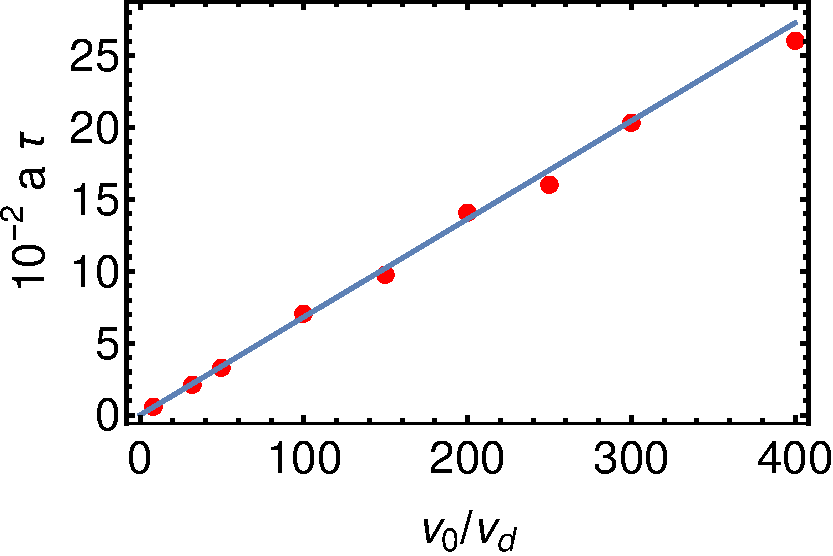
\includegraphics[width=0.48\linewidth]{Figures/asym_fig_t_a_param1.pdf}
  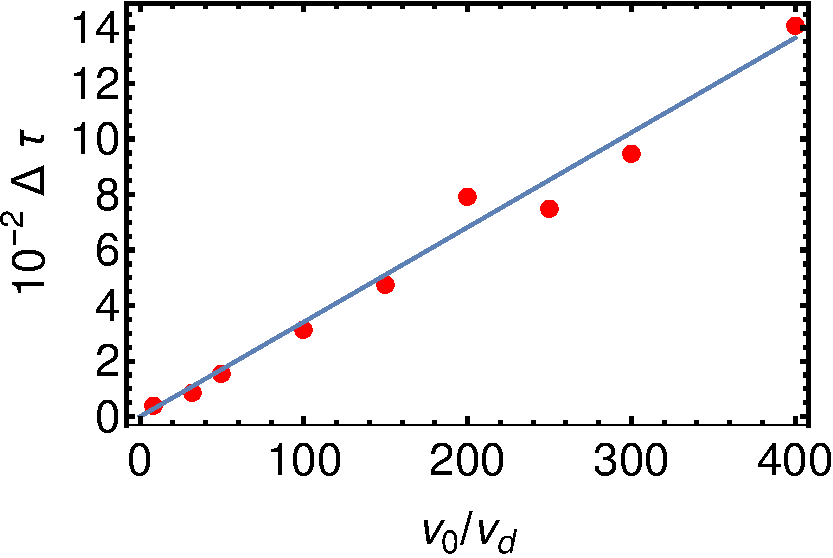
\includegraphics[width=0.48\linewidth]{Figures/asym_fig_t_a_param2.pdf}
  \end{center}
  \caption{Asymmetric ${\cal T/A}$ device with symmetry VIII: comparison between numerically achieved parameters (red dots) and approximated parameters (blue, solid lines) versus velocity $v_0$.
  (a) Height of Rabi frequency $a$, (b) detuning $\Delta$.
  \label{fig_t_a_param}}
\end{figure}
% ------------------------------------------------------------------------------

%
%
%
%

%
%
\section{Discussion\label{sec:chapter3_Discussion}}

Since devices of technological interest, such as one-way filters for transmission or reflection, one-way barriers, one-way mirrors, and others, may be built based on the asymmetric scattering response of non-Hermitian Hamiltonians, there is both fundamental
interest and applications in sight to implement non-Hermitian scattering Hamiltonians. The results in this chapter are a step forward in that direction, specifically I propose a quantum-optical implementation of potentials with asymmetric scattering response.
They are non-local and non-PT symmetrical, which allows for asymmetric transmission.

In general the chosen Hilbert space may  be regarded as a subspace of a larger space. For example,  the space of a ``structureless particle'' in 1D is the ground-state subspace
for a particle with internal structure, consisting of two-levels in the simplest scenario.
It is then possible to regard the non-Hermitian physics in the reduced space
as a projection of the larger space, which may itself be driven by a  Hermitian or a non-Hermitian Hamiltonian.
I have used the Hermitian option in the examples, where I assumed a zero decay constant, $\gamma=0$, for the excited state.
A non-zero $\gamma$ implies  a non-Hermitian  Hamiltonian in the larger two-level space. The description may still be
enlarged,  including  quantized field modes to account for the atom-field interaction with a Hermitian Hamiltonian.
As an outlook, depending on the application, there might be the need for a more fundamental and detailed descriptive level. Presently I discuss the desired physics (i.e., the scattering asymmetries) at the level of the smallest 1D space of the ground state, while taking refuge in the
two-level space to find a feasible physical implementation.
    % Physical Implementation of non-Hermitian and non-local Hamiltonians


% ------------ PART II: Heat Rectification ---------------------------------------------------------
\part{Heat rectification in mesoscopic systems\label{partII}}
%!TEX root = ../Thesis.tex
%Chapter 4

\chapter{Local Rectification of Heat Flux}
\label{Chapter4}
\lhead{Chapter 4. \emph{Local Rectification of Heat Flux}} % Write in your own chapter title to set the page header
%
In this chapter, a model for an atom-chain thermal rectifer is presented. The atoms in the chain are trapped in on-site harmonic potentials, and interact with their nearest neighbours by Morse potentials (or also by harmonic potentials in a simplified version). The chain is homogeneous except for a local modification of the interactions at one site, the ``impurity''. The rectification mechanism is due here to the localized impurity, the only asymmetrical element of the structure, apart from the externally imposed temperature bias, and does not rely on putting in contact different materials or other known mechanisms such as grading or long-range interactions.  The effect survives if all interaction forces are linear except the ones for the impurity.

The rest of the chapter is organized as follows. In section \ref{sec:homogeneous_chain} I shall describe the homogeneous 1D chain, without the impurity.  For this system, I numerically solve the dynamical equations, to show that the usual heat conduction applies. In section \ref{sec:Impurity_rectifier} I modify the potentials for one of the atoms and demonstrate the rectification effect. I also observe rectification when all the interaction Morse potentials are substituted by harmonic oscillators. Finally, in section \ref{sec:chapter4_Discussion} I summarize and discuss the results of this chapter.

\section{Homogeneous one-dimensional chain\label{sec:homogeneous_chain}}

I start with a homogeneous $1D$ chain with $N$ atoms coupled at both extremes to heat baths, at different temperatures $T_h$ and $T_c$ for ``hot" and ``cold" respectively. The baths are modeled with a Nos\' e-Hoover method as described in \cite{Martyna1992}. Atoms $1$ and $N$ represent the first and the $N$-th atom in the chain, from left to right, that will be in contact with the baths. All the atoms are subjected to on-site potentials and to nearest-neighbor interactions, and their equilibrium positions $y_{i0}$ are assumed to be equally spaced by a distance $a$.
$x_i= y_i-y_{i0}$,
$i=1,...,N$, represent the displacements from the equilibrium positions of the corresponding atoms
with positions $y_i$.

%%%%%%%%%%%%%%%%%%%%%%%
\begin{figure}
\centering
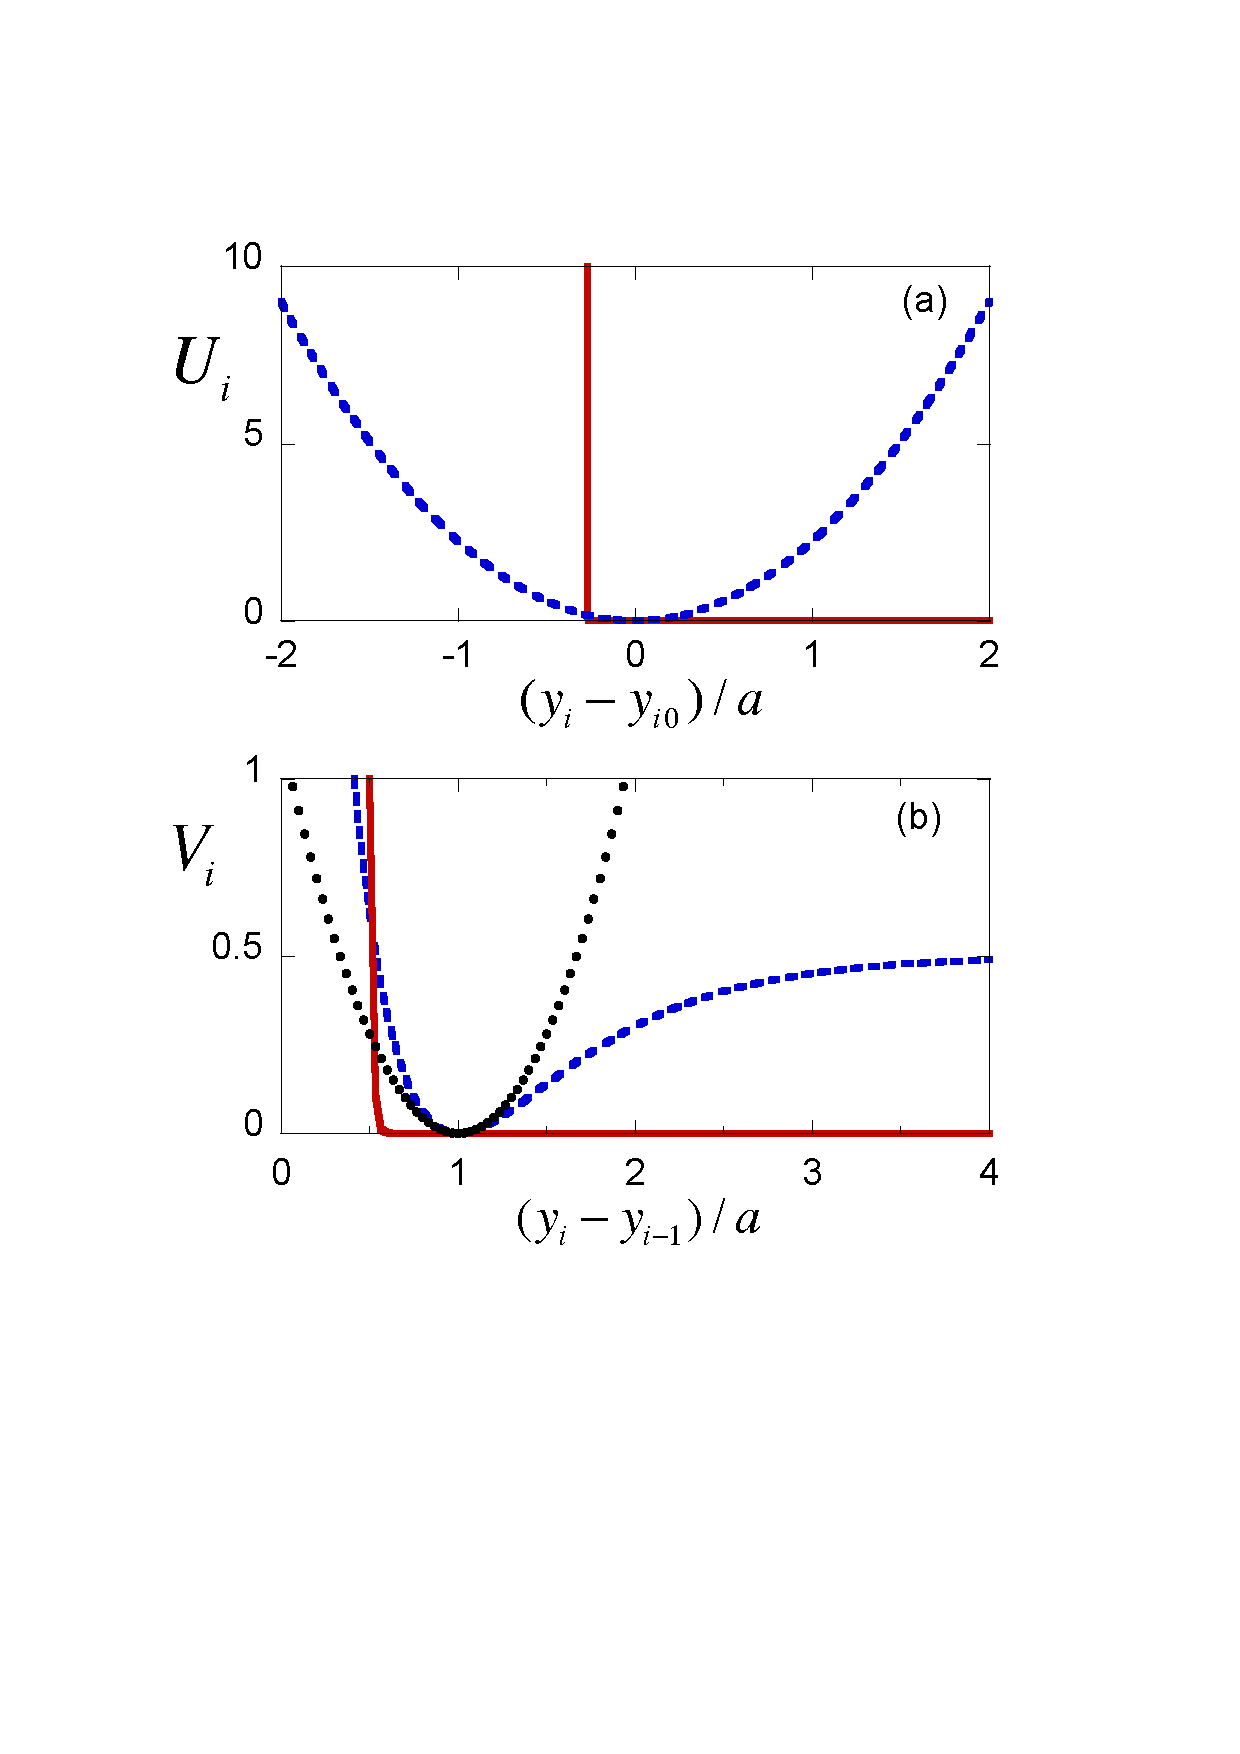
\includegraphics[width=0.65\linewidth]{Figures/FIG1.pdf}
\caption{(a) On-site potentials: harmonic potential centered at the equilibrium position of each atom (dashed blue line) as a function of the displacement from this position $x_i=y_i-y_{i0}$ in $a-$units, and the on-site potential for the impurity, $i=N/2+1$
($N$ even, red solid line). (b) Interaction potentials as a function of the distance between nearest neighbors: Morse potential
(blue dashed line) valid for all atoms except for $i=N/2+1$, $N$ even, where the modified potential (red solid line) is used.
The harmonic approximation of the Morse potential is also depicted (eq. (\ref{Vhar}), black dots, only used for fig. \ref{fig:chapter4_figure5}, below).
Parameters: $D=0.5$, $g=1$, $\gamma = 45$, $d=100$ and $b=105$, used throughout the chapter.
}
\label{fig:chapter4_figure1}
\end{figure}
%%%%%%%%%%%%%%%%%%%%%%%%%

The classical Hamiltonian of the atom chain can be written in a general form as
%
\begin{equation}
\label{GH}
%GH=general Hamiltonian
H=\sum_{i=1}^{N} H_i,
\end{equation}
%
with
%
\begin{eqnarray}
\label{GH2}
%GH=general Hamiltonian
H_1&=&{{p^2_1} \over {2m}} +U_1(x_1)+V_L,
\nonumber\\
H_i&=&{{p^2_i} \over {2m}} +U_i(x_i)+V_i(x_{i-1},x_i)  \quad i=2,...,N-1,
 \nonumber\\
H_N&=&{{p^2_N} \over {2m}} +U_N(x_N)+V_N(x_{N-1},x_N) + V_R,
\end{eqnarray}
%
where the $p_i$ are the momenta, $U_i(x_i)$ is the on-site potential for the $i$th atom, and $V_i(x_{i-1},x_i)$ represents the atom-atom interaction potential. $V_R$ and $V_L$ are the interactions coupling the boundary atoms to the Nos\'e-Hoover thermostats, see \cite{Martyna1992}.

%%%%%%%%%%%%%%%%%%%%%%%%%%%%
\begin{figure}
\centering
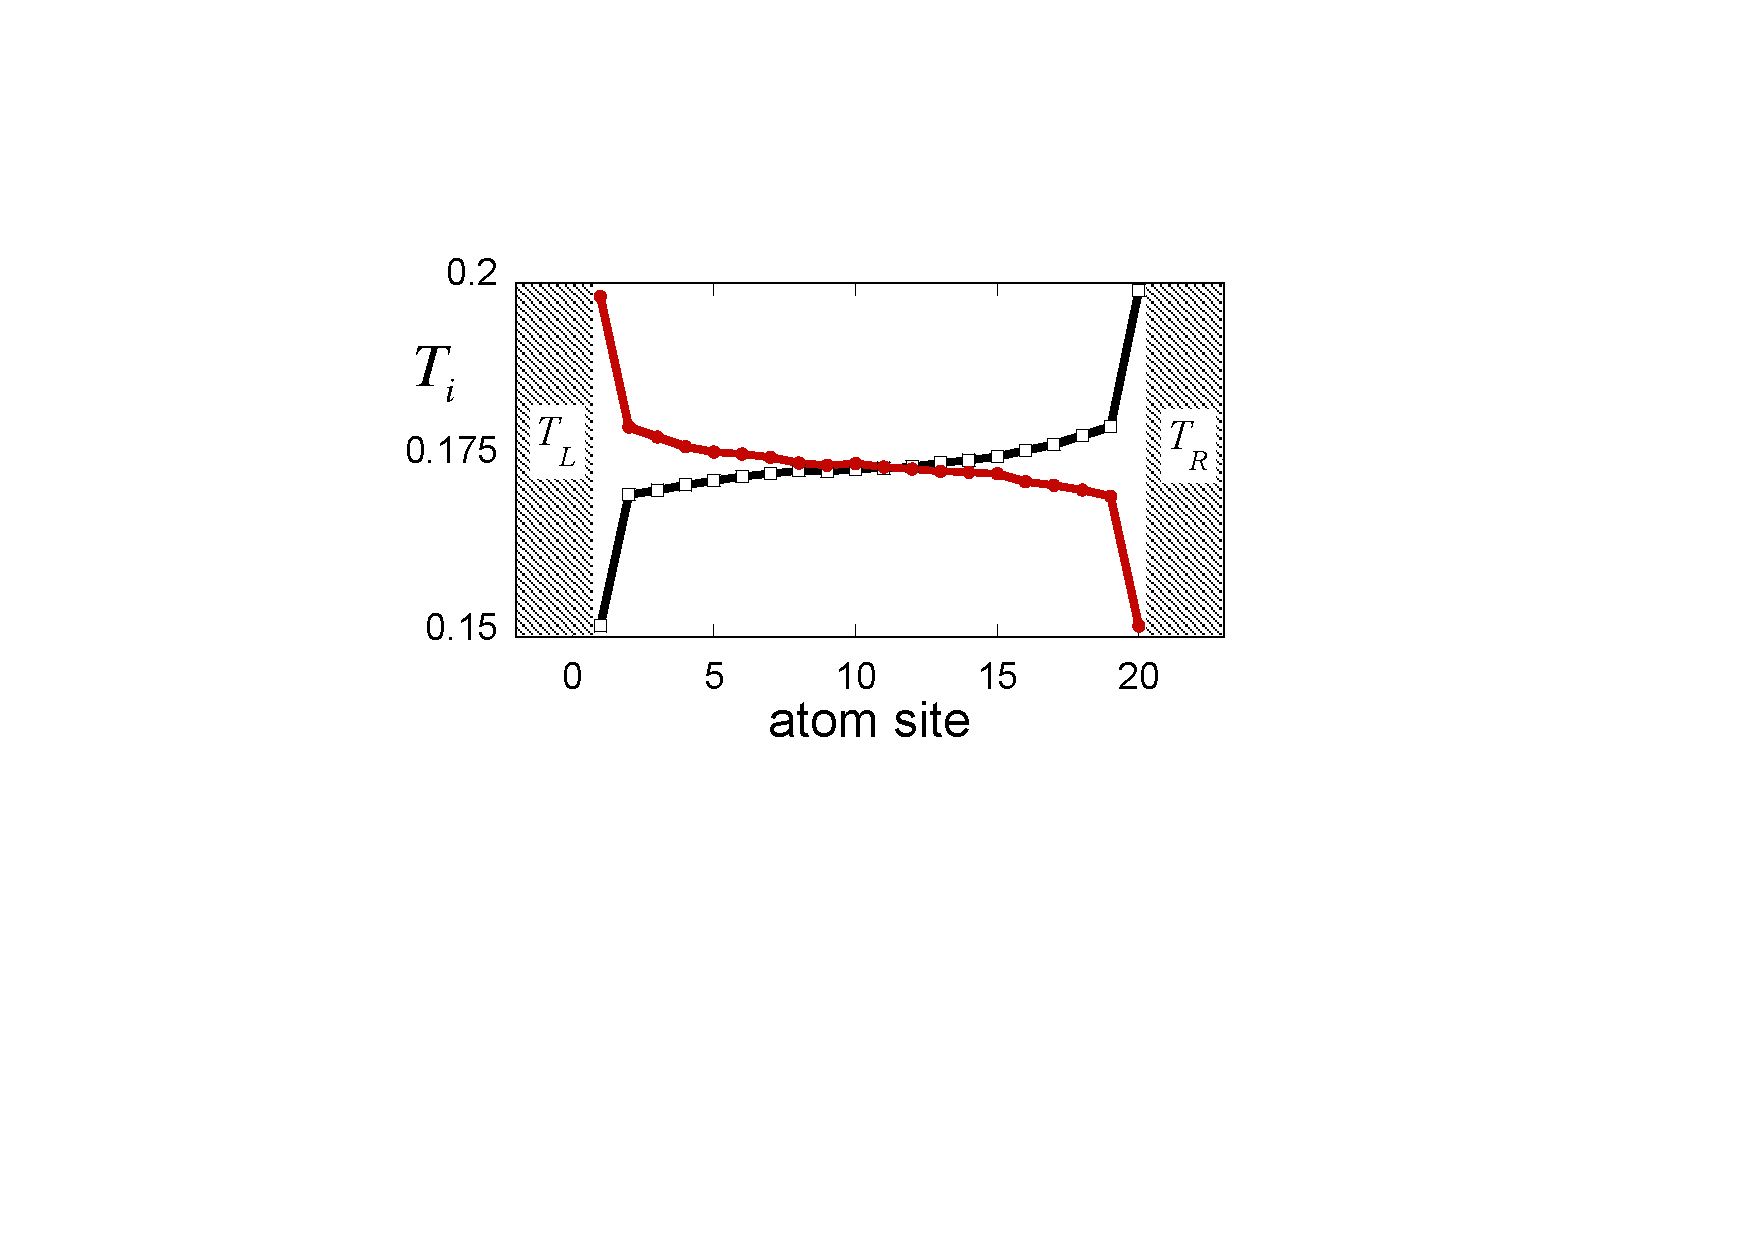
\includegraphics[width=0.65\linewidth]{Figures/FIG2.pdf}
\caption{Symmetric temperature profiles for a homogeneous chain, without impurity.  For $T_{h}=T_{L}$, $T_c=T_R$ (red solid dots) the (absolute value of) the heat flux is $J_{L\rightarrow R}$, equal to $J_{R\rightarrow L}$ for the reverse configuration of the bath temperatures, $T_{h}=T_{R}$, $T_c=T_L$
(black empty squares). Parameters as in fig. \ref{fig:chapter4_figure1}.}
\label{fig:chapter4_figure2}
\end{figure}
%%%%%%%%%%%%%%%%%%%%%%%%%%%%%%

There are a large number of $1D$ models that obey this general Hamiltonian. Different choices of the trapping and interaction potentials would give different conductivity behaviors. I choose a simple form of the Hamiltonian in which each atom is subjected to a harmonic on-site potential and a Morse interaction potential between nearest neighbors (see fig. \ref{fig:chapter4_figure1}, dashed lines),
%
\begin{eqnarray}
\label{HO}
%HO=Harmonic oscillator
U_i(x_i)&=&{1 \over 2} m \omega^2 x^2_i,
%\end{equation}
%\begin{equation}
\\
\label{IH}
%IP=Interaction potential
V_i(x_{i-1},x_i)&=&D\left \{e^{-\alpha [x_i-x_{i-1}]}-1\right \}^2,
\end{eqnarray}
%
where $\omega$ is the trapping angular frequency, and $D$ and $\alpha$ are time independent parameters of the Morse potential.
A ``minimalist version'' of the model where $V$ becomes the harmonic limit of eq. (\ref{IH}), dotted line in fig. 1,
 will also be considered in the final discussion,
%
\begin{equation}
\label{Vhar}
{V}_i(x_{i-1},x_i)=k(x_i-x_{i-1})^2/2,\;k=2D\alpha^2.
\end{equation}
%
For convenience, dimensionless units are used and the mass of all particles is set to unity.

I start by studying the homogeneous configuration with no impurity and potentials (\ref{HO}) and (\ref{IH}), solving numerically the dynamical equations for  the Hamiltonian (\ref{GH}) with a Runge-Kutta-Fehlberg algorithm. I have chosen a low number of atoms, $N=20$,  with thermal baths at $T_h=0.20$ and $T_c=0.15$ at both ends of the chain with 16 thermostats each. The real temperature is related to the dimensionless one through $T_{real}=T m a^2 \omega^2/k_B$ so, for typical values  $m\approx10^{-26}$ kg, $\omega \approx 10^{13}$ s$^{-1}$, $a\approx 10^{-10}$ m, and using $k_B =1.38 \times 10^{-23}$ JK$^{-1}$,
the dimensionless temperatures $0.15,\, 0.20$, translate into $100,\, 150$ K. It is advisable to use temperatures around these values in order to ensure that the displacements of the particles are realistic \cite{Casati1984}.

%%%%%%%%%%%%%%%%%%%%%%%%%%%%%%%%%%
\begin{figure}
\centering
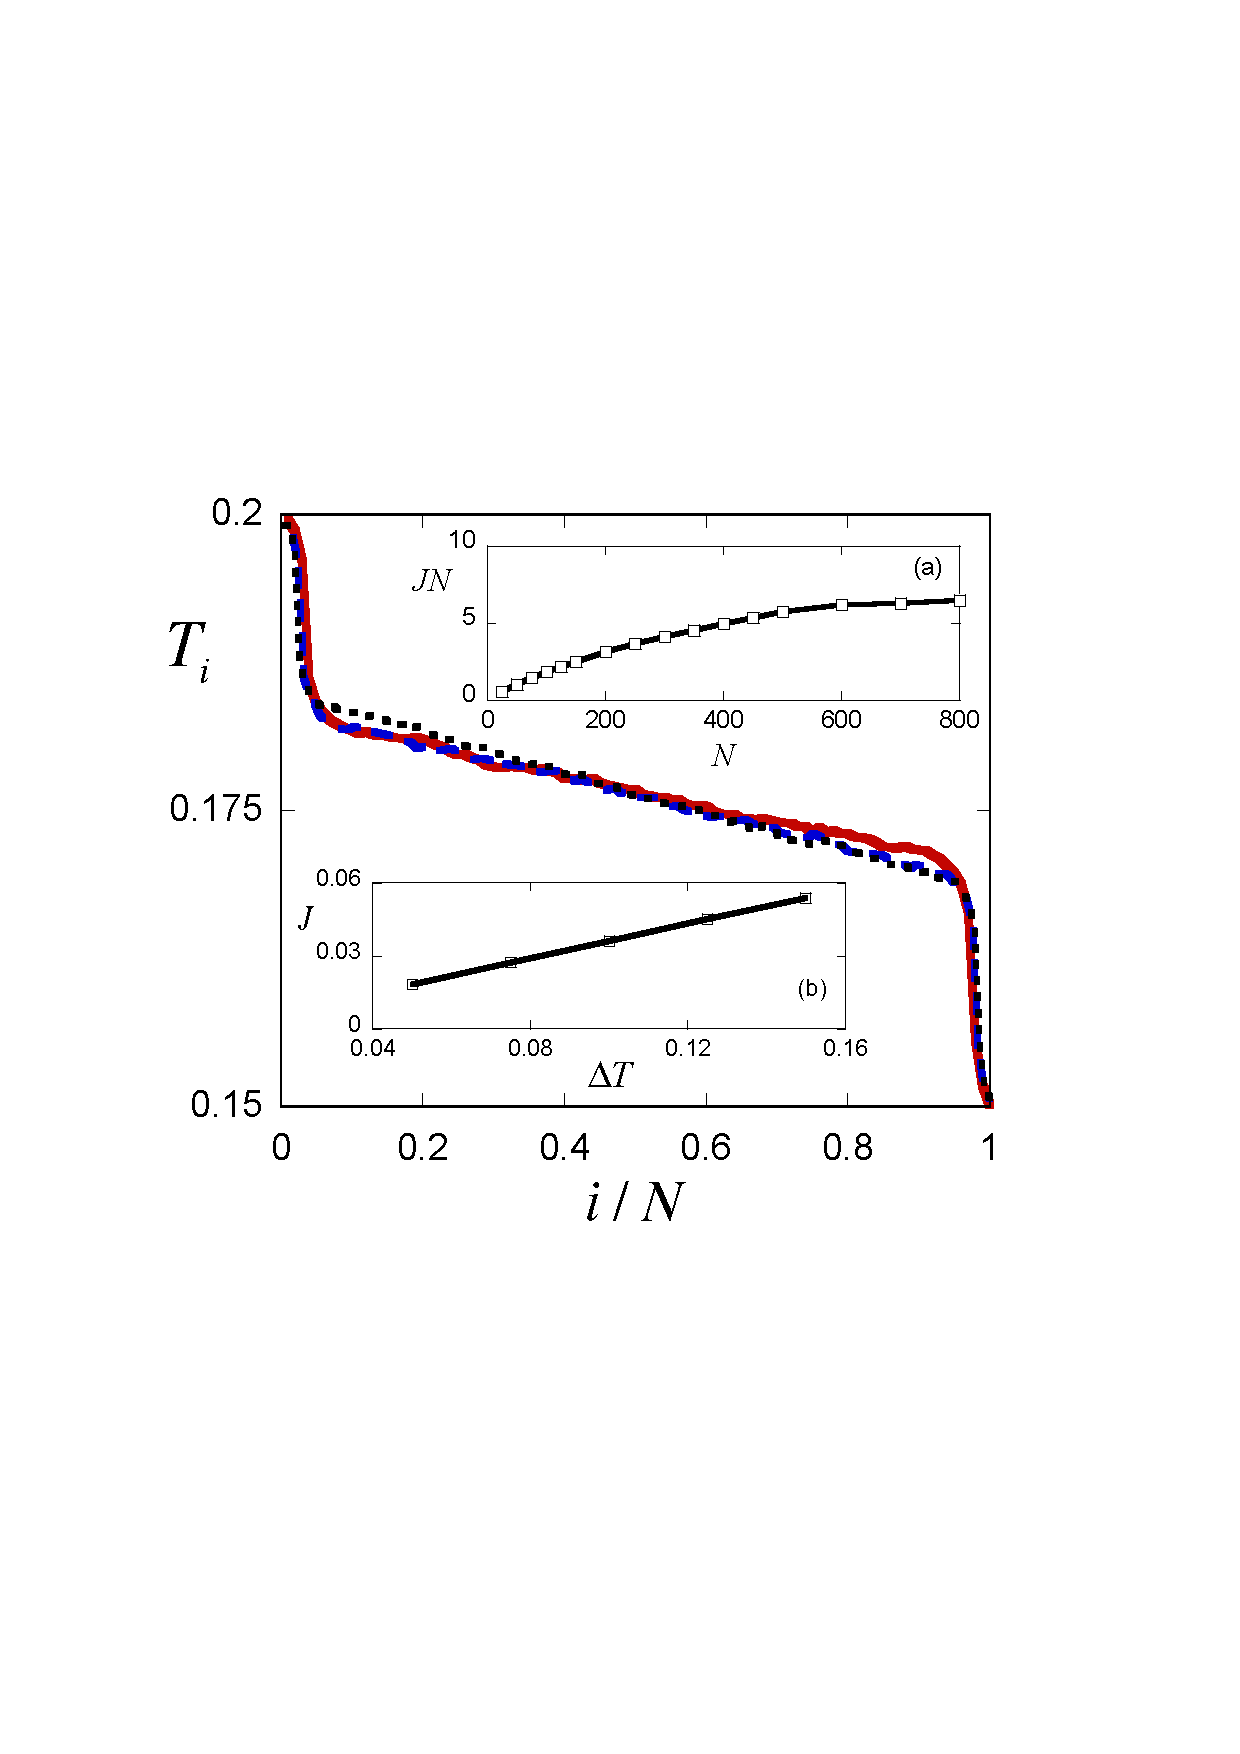
\includegraphics[width=0.65\linewidth]{Figures/FIG3.pdf}
\caption{Temperature profile along the homogeneous chain for different number of atoms: 100 (dotted black line), 125 (dashed blue line) and 150 (solid red line). The atom sites have been rescaled with the total number of atoms.
%, showing the convergence of the spatial profile of the local temperature $T_i$.
The time averages have been carried over a time interval of $\approx 2 \times 10^6$ after a transient of $\approx 1\times 10^5$. In the inset (a), the product $JN$ vs. $N$ demonstrates that for long chains $JN$ is independent of $N$. In (b) the linear dependence of $J$ with $\Delta T$ for a fixed number of atoms, $N=100$, is shown. Parameters as in fig. \ref{fig:chapter4_figure1}.}
\label{fig:chapter4_figure3}
\end{figure}
%%%%%%%%%%%%%%%%%%%%%%%%%%%%%%%%%%%%%%%%

First I demonstrate the conductivity behavior of the model.
%that our system satisfies Fourier's heat law for the heat flux, $J=\kappa \nabla T$.
%, so it shows normal thermal conductivity. ESTE CONCEPTO TIENE QUE VER CON EL TAMA�O?
To this end, I calculate the local heat flux $J_i$ and temperature $T_i$, performing the numerical integration
%of Eq. (\ref{GH2})
for long enough times to reach the stationary state.
The local temperature is found as the time average $T_i= \langle p_i^2 / m \rangle$, whereas
%After a transient, the local temperature is given by the time average $T_i=\langle p_i^2\rangle$.
$J_i$,  from the continuity equation
%, $\dot H(x,t)+divJ(x,t)=0,$
\cite{Hu1998}, is given by
%
%Fourier law: temperature gradient vanishes with N
\begin{equation}
\label{heatflux}
J_i=-\dot x_i {{\partial V(x_{i-1},x_{i})} \over {\partial x_i}}.
\end{equation}
%
From now on I only consider the time average $\langle J_i (t)\rangle$, which converges to a constant value for all sites once the system is in the stationary nonequilibrium state. I depict the temperature profiles, for $N=20$, first with $T_L=T_h$ and $T_R=T_c$
($L$ and $R$ stand for left and right) and after switching the positions of the thermal baths in fig. \ref{fig:chapter4_figure2}. The profiles are symmetric, as expected, and the heat flux does not have a preferred direction  \cite{Hu1998,Terraneo2002}. Denoting the absolute values of the fluxes from the left (when $T_L=T_h$) as
$J_{L\rightarrow R}$, and from the right (when $T_R=T_h$) as
$J_{R\rightarrow L}$, I find that $J_{L\rightarrow R}=J_{R\rightarrow L}=J=1.6\times 10^{-2}$, in the dimensionless units, consistent with the values found in other models \cite{Terraneo2002,Hu1998}.

%%%%%%%%%%%%%%%%%%%%%%%%%%%%%%%%%%%
\begin{figure}
\centering
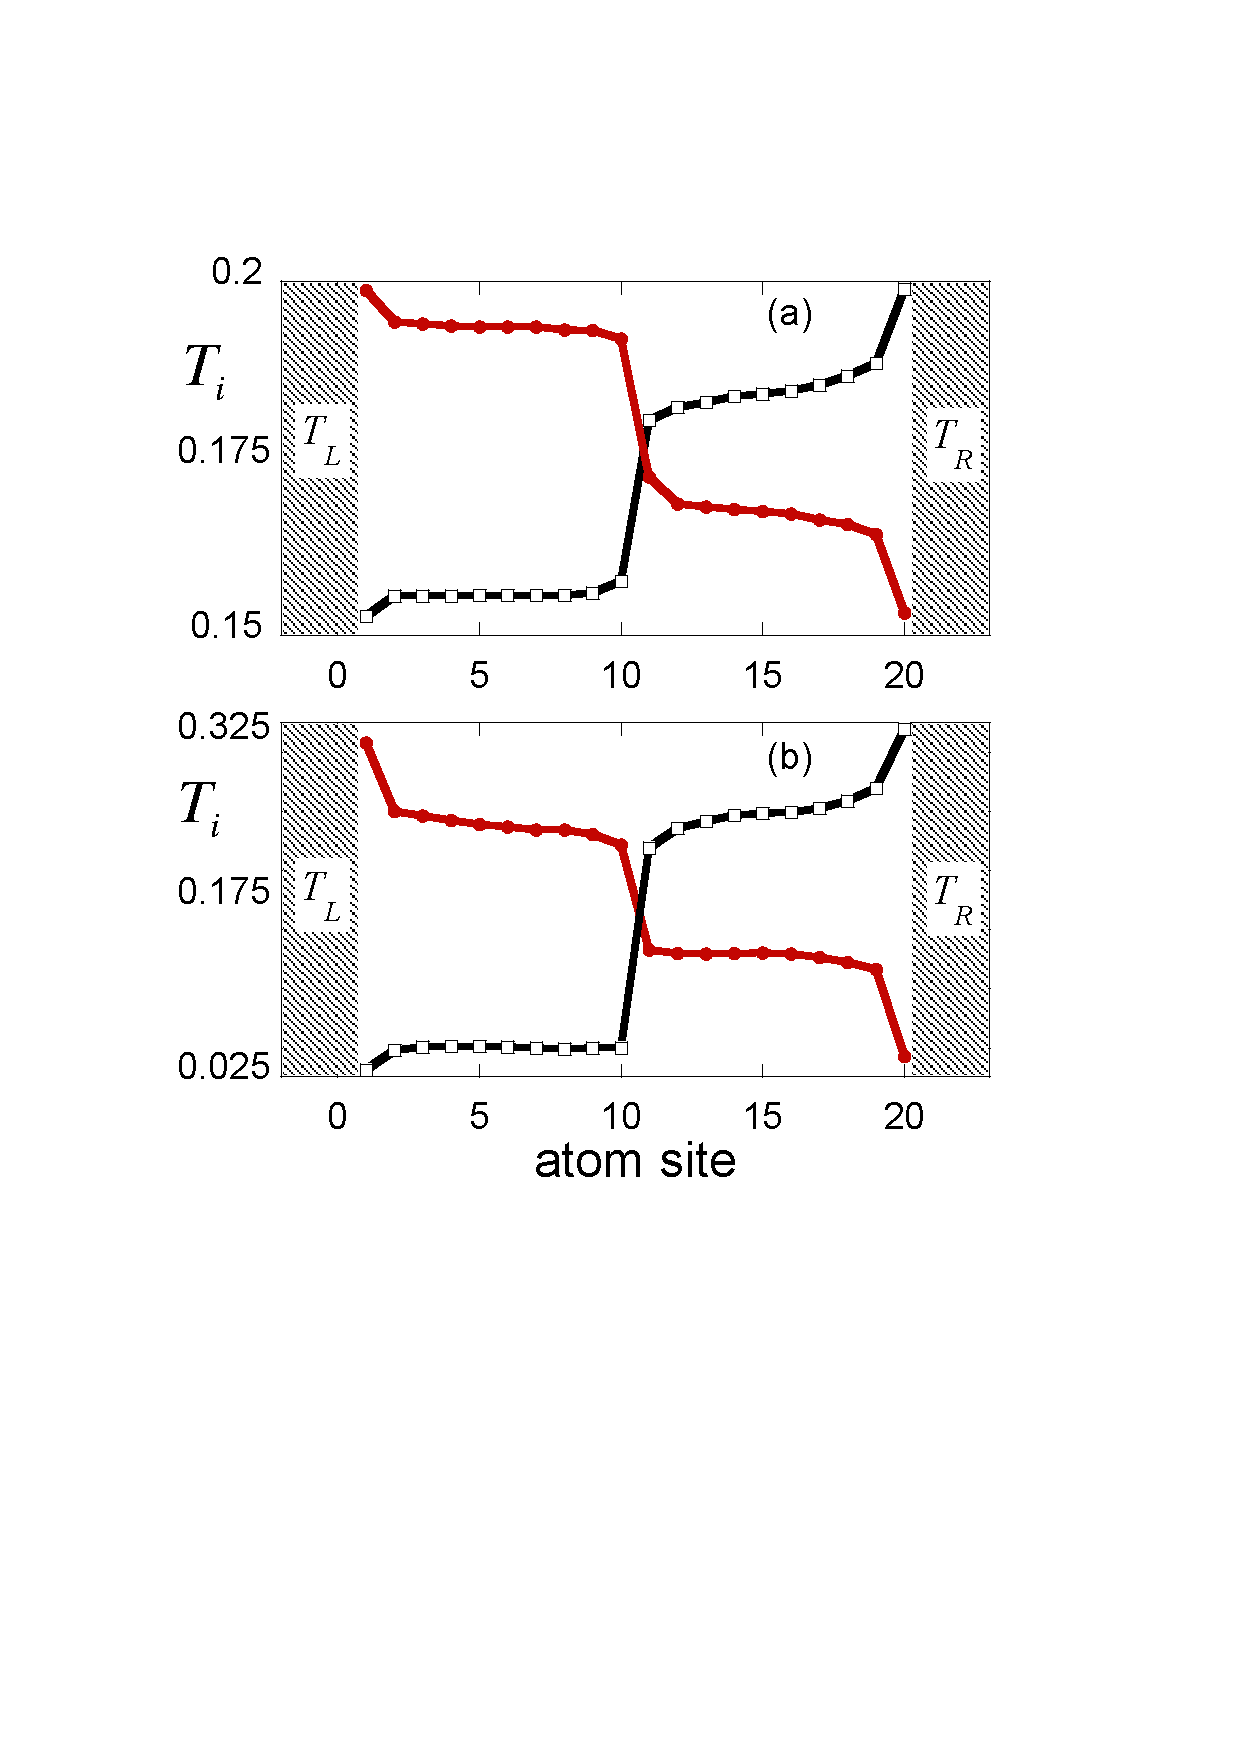
\includegraphics[width=0.65\linewidth]{Figures/FIG4b.pdf}
\caption{Temperature profile for the chain of $N=20$ atoms, with an impurity in the $N/2+1$ position, with $T_L=T_h$ and $T_R=T_c$ (circles) and with the thermostat baths switched (squares).
Parameters as in fig. \ref{fig:chapter4_figure1}.
(a) $T_c=0.15$, $T_h=0.2$. $J_{L\rightarrow R}=0.00769$ vs $J_{R\rightarrow L}=0.00581$, with gives a rectification $R=31 \% $; (b) $T_c=0.025$, $T_h=0.325$. $J_{L\rightarrow R}=0.0499$ vs  $J_{R\rightarrow L}=0.0140$, with $R=256 \%$.}
\label{fig:chapter4_figure4}
\end{figure}
%%%%%%%%%%%%%%%%%%%%%%%%%%%%%%%%%%%%%%%%%

The profile of the temperature is linear with boundary nonlinearities at the edges, close to the thermal baths,  due to the boundary conditions \cite{Lepri1997}. In fig. \ref{fig:chapter4_figure3} I depict $T_i$ vs $i/N$ for $N=100, 125$ and $150$ with the same boundary conditions. For these
larger atom numbers  I have connected the first 3 and the last 3 atoms to the Nos\'e-Hoover baths.
%The temperature gradient scales as $N^{-1}$, which is also true for many other different models \cite{Hu1998}.
In the inset (a) of fig. \ref{fig:chapter4_figure3}  the product $JN$ is plotted vs. $N$ showing that in a low $N$ limit there is a well defined conductivity per unit length whereas for longer chains, $JN$ tends to be constant  which indicates a normal thermal conductivity independent of the length. Fixing the number of atoms to 100, as in the inset (b) of fig. \ref{fig:chapter4_figure3},  I observe a linear dependence between the flux and $\Delta T$.
%Fourier law, $J=\kappa \nabla T$, is fulfilled.

\section{Impurity-based thermal rectifier \label{sec:Impurity_rectifier}}

To rectify the heat flux I modify the potentials for site $j=N/2+1$ with $N$ even, as
%
%\begin{equation}
%\label{IMP1}
%IMP1=impurity in absolute position
%U_j(y_j,t)=d e^{-b [y_j(t)-y_{d}]} +ge^{-\gamma [y_j(t)-y_{j-1}(t)-\epsilon]}
%\end{equation}
%with $y_{d}=y_{d,0}-a/3$.  Written in terms of the displacements, $x_j$,
%
\begin{eqnarray}
\label{IMP}
%IMP=impurity
U_j(x_j,t)&=&d e^{-b [x_j(t)+a/3]},
\\
V_j(x_{j-1},x_j,t)&=&ge^{-\gamma [x_j(t)-x_{j-1}(t)+a/2]}.
\end{eqnarray}
%
All the parameters involved, $d, b$, and $g,\gamma$ are time independent. In fig. \ref{fig:chapter4_figure1} the modifications introduced with respect to the ordinary sites are shown (solid lines).  The different on-site and interaction terms introduce soft-wall potentials
(instead of hard-walls to aid integrating the dynamical equations) that make it difficult for the impurity to transmit its excitation to the left whereas left-to-right transmission is still possible.
This effect is facilitated by the relative size of the coefficients, $a/3<a/2$, that determine the position of the walls.
% that I fixed after some experimentation.
These positions imply that an impurity excited by a hot right bath cannot affect its left cold neighbour near its equilibrium position at the $j-1$ site.
However, if the left $j-1$ atom is excited from a hot bath on the left,
it can get close enough to the impurity to kick it and transfer kinetic energy.

\begin{figure}
\centering
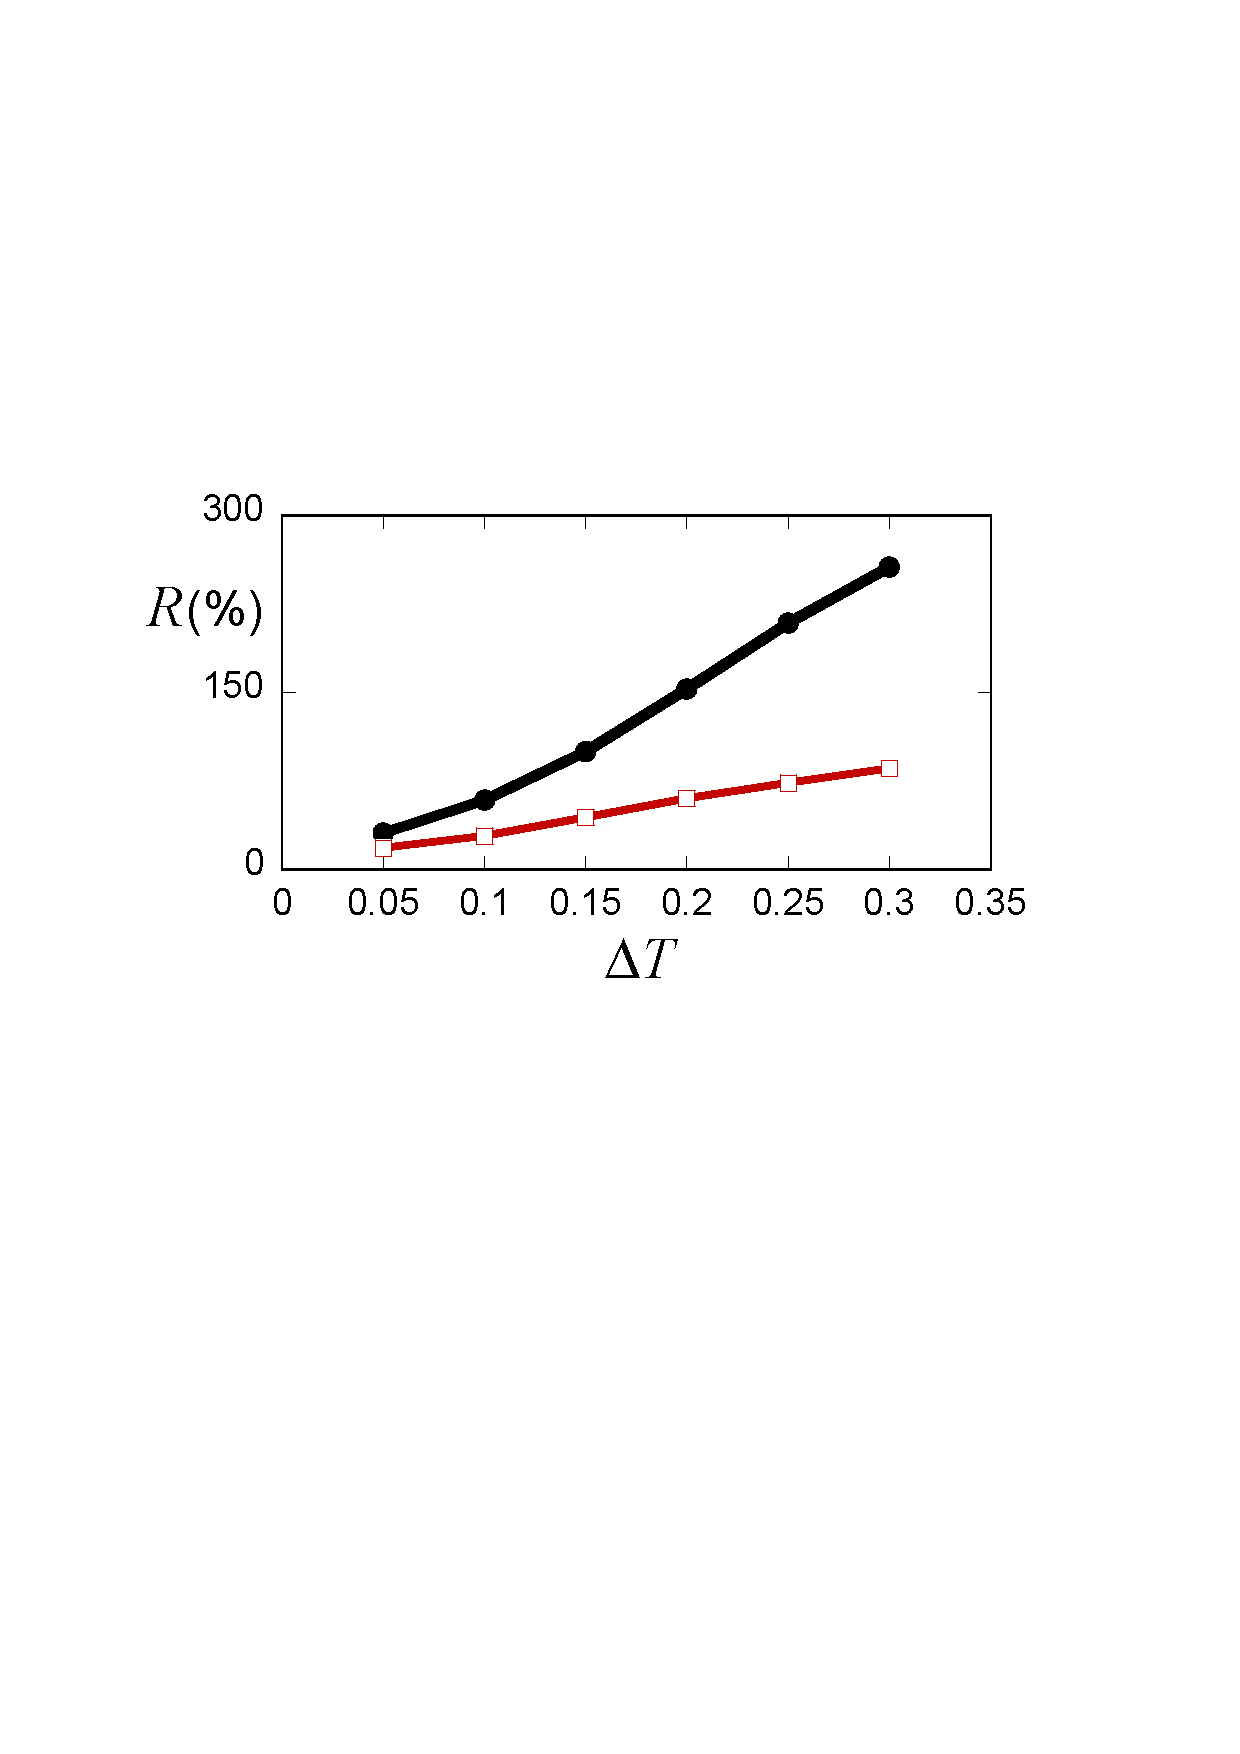
\includegraphics[width=0.65\linewidth]{Figures/FIG5new.pdf}
\caption{Rectification factor $R$ as a function of the temperature difference between ends of the chain of atoms, $\Delta T$.
%The rectification factor shows a very strong dependency on $\Delta T$.
I have changed both $T_h$ and $T_c$ according to $T_c=0.15-(\Delta T-0.05)/2$ and $T_h=0.2+(\Delta T-0.05)/2$, with $N=20$,  keeping the rest of parameters as in fig. \ref{fig:chapter4_figure1}.
Interatomic potentials: Morse potential, eq. (\ref{IH}) (black line with circles, see the temperature profiles of extreme points in fig. \ref{fig:chapter4_figure4}); harmonic potential, eq. (\ref{Vhar}) (red line with squares).}
\label{fig:chapter4_figure5}
\end{figure}

After extensive numerical simulations, I have chosen the values of these parameters as in fig. \ref{fig:chapter4_figure1}, such that the conductivity in the forward direction, $J_{L\rightarrow R}$, and the rectification factor, defined as $R=(J_{L\rightarrow R}-J_{R\rightarrow L}) / J_{R\rightarrow L}\times 100$,
are both large for $T_h=0.2$, $T_c=0.15$. A large $R$ without a large $J_{L\rightarrow R}$ could in fact be useless \cite{Roberts2011}.
%($R=0$ would represent a perfectly symmetric heat conduction.).
Note that the parameters are not necessarily the optimal combination, which in any case would depend on the exact definition of ``optimal'' (technically on how $J_{L\rightarrow R}/J$ and $R$ are weighted and combined in a cost function and on the limits imposed on the
parameter values). This definition is an interesting question but it goes beyond the focus of this chapter, which is to demonstrate and discuss the effect of the localized inpurity.

I have used again $N=20$ atoms connected to baths of 16 thermostats each, with the same temperatures as for the homogeneous chain, and numerically solved the dynamical equations
to calculate the local temperature and the heat flux for both configurations of the baths. The interatomic potential for the regular atoms is the Morse potential (\ref{IH}).
In fig. \ref{fig:chapter4_figure4}(a), the temperature profiles show a clear asymmetry between ${L\rightarrow R}$ and ${R\rightarrow L}$. Specifically, I find $J_{L\rightarrow R}=7.6 \times 10^{-3}$ and $J_{R\rightarrow L}=5.8 \times 10^{-3}$ which gives
$R=31\%$. The effect decays with longer chains,  with, for example, $R=19\%$ for $N=100$, and R=17.8\% for $N=150$.

\begin{figure}
\centering
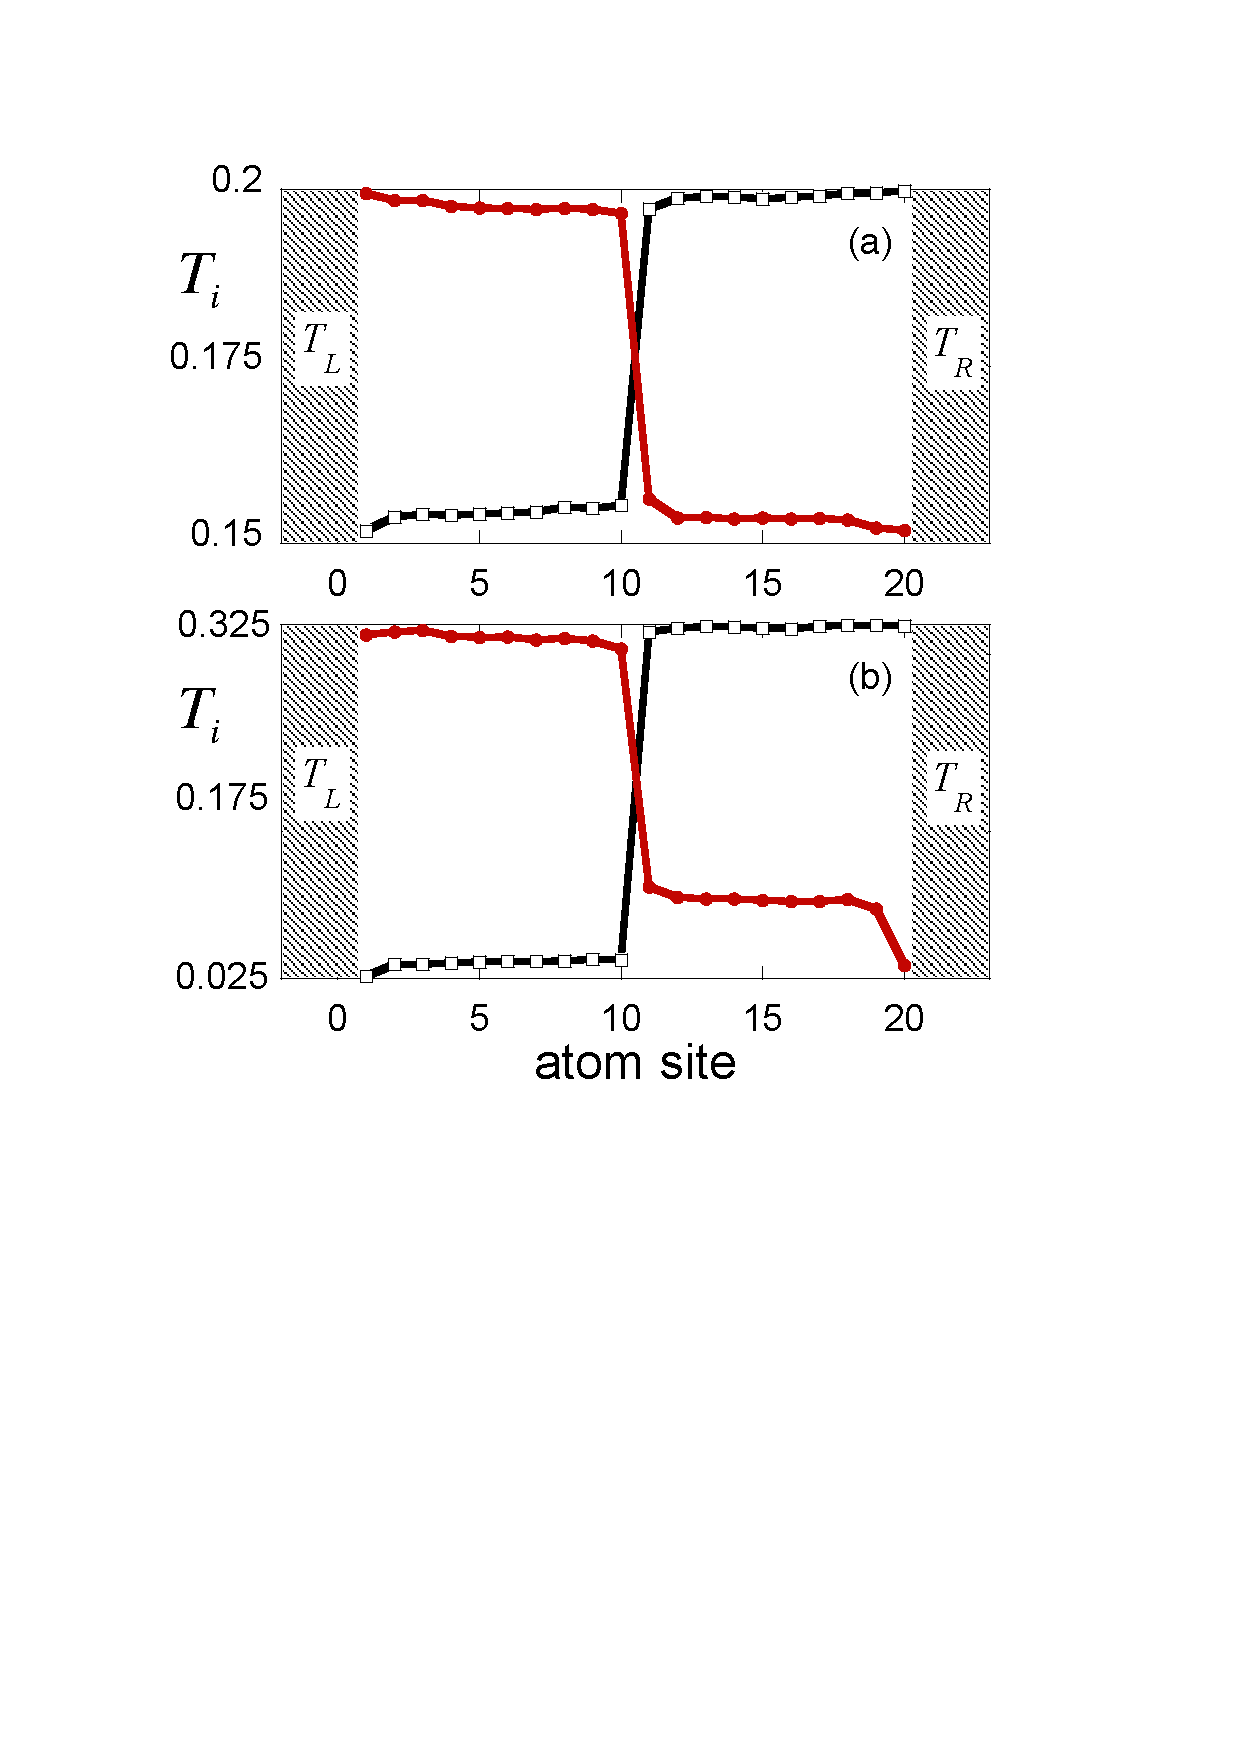
\includegraphics[width=0.65\linewidth]{Figures/FIG6.pdf}
\caption{Temperature profile for a harmonic interacting chain of $N=20$ atoms, with an impurity in the $N/2+1$ position, with $T_L=T_h$ and $T_R=T_c$ (circles) and with the thermostat baths switched (squares), for (a) $\Delta T = 0.05$ and (b)  $\Delta T = 0.3$. The corresponding rectification factors are (a) $R=18\%$ and (b) $R=85\%$. Parameters regarding the impurity are the same as in fig. \ref{fig:chapter4_figure1}.
}
\label{fig:chapter4_figure6}
\end{figure}

These temperature profiles depend on the difference between the bath temperatures, see e.g. fig. \ref{fig:chapter4_figure4}(b). Increasing the temperature gap, but  keeping $T_h$ low enough so that the displacement of the atoms from their equilibrium positions is realistic, I find higher values of $R$. Figure \ref {fig:chapter4_figure5} shows the strong dependence of $R$ with $\Delta T$ (black circles). I have changed both $T_h$ and $T_c$ so that the mean temperature $(T_c+T_h)/2$ remains constant.

\section{Discussion\label{sec:chapter4_Discussion}}

I have presented  a scheme for thermal rectification using a one-dimensional chain of atoms which is homogeneous except
for the special interactions of one of them, the impurity, and the couplings with the baths at the boundaries. These proof-of-principle results for an impurity-based rectification mechanism may encourage further exploration of the impurity-based rectification, in particular of the effect of different forms for the impurity on-site potential and its interactions with neighboring atoms.
In contrast to the majority of chain models, the structural asymmetry in the present model is only in the impurity. The idea of a localized effect was already implicit in early works on a two-segment Frenkel-Kontorova
model \cite{Li2004,Hu2006}, where rectification depended crucially on the interaction constant coupling between the two segments.
However, the coupling interaction was symmetrical and the asymmetry was provided by the different nature
(parameters) of the segments put in contact.
Also different from common chain models are the potentials chosen here. Instead of using the Morse potential as an on-site model, see e.g.  \cite{Terraneo2002},
I have considered a natural setting where this potential characterizes the interatomic interactions,
and the on-site potential is symmetrical with respect to the equilibrium position, and actually harmonic.
The numerical results indicate that this model is consistent with normal conduction,
and also helps to isolate and identify the local-impurity mechanism for rectification.
In this regard it is useful to consider a further simplification, in the spirit of the minimalists models
proposed by Pereira \cite{Pereira2017}, so as to distill further the essence of the local rectification mechanism.
If the Morse interatomic interaction is substituted by the corresponding harmonic interaction, see the black dotted line in fig. \ref{fig:chapter4_figure1}(b), the rectification effect remains, albeit slightly reduced, see fig. \ref{fig:chapter4_figure5}. The chain is then perfectly linear with the only nonlinear exception  localized
at the impurity.
The temperature dependent feature mentioned in \cite{Pereira2017} as the second necessary condition for rectification besides asymmetry, is here localized in the impurity too, and consists of a different
capability to transfer kinetic energy depending on the temperatures on both sides of the impurity.
Figure \ref{fig:chapter4_figure6} shows temperature profiles for the purely harmonic chain to be compared with the Morse-interaction
chain in fig. \ref{fig:chapter4_figure4}. Flatter profiles are found on both sides of the impurity, as corresponds to the abnormal transport expected for harmonic chains \cite{Lepri2003}. It would be interesting to combine the impurity effect with other rectification mechanisms (such as grading, long-range interactions, or use of different segments), or with more impurities in series to enhance further the rectification effect.

Even though the motivation was to mimic the effect of a localized atom diode that lets atoms pass only one way,
unlike the atom diode \cite{Ruschhaupt2004}, all interactions in the present model
are elastic. The model may be extended by adding an irreversible,  dissipative element so as to induce not only rectification but a truly Maxwell demon for heat transfer \cite{Skordos1992,Ruschhaupt2006}.
On the experimental side, one dimensional chains of neutral atoms in optical lattices can be implemented with cold atoms \cite{Bloch2005}.
An impurity with different internal structure could be subjected to a different on-site potential imprinted by a holographic mask \cite{Bakr2009}, and asymmetrical interatomic interactions could be implemented by trapping a controllable polar molecule or mediated by atoms in parallel lattices \cite{Gollub2014}.
    % Heat Rectification with local impurities
%!TEX root = ../Thesis.tex
%Chapter 5

\chapter{Asymmetric heat transport in ion crystals}
\label{Chapter5}
\lhead{Chapter 5. \emph{Asymmetric heat transport in ion crystals}} % Write in your own chapter title to set the page header

In this chapter I propose to bridge the gap between mathematical models and actual physical systems by exploring the implementation of a thermal rectifier in a realistic, graded system with long-range interactions:
a chain of ultracold ions in a segmented Paul trap with frequency-graded microtraps for each ion. Long-range interactions are due to the Coulomb forces, and the baths at the ends of the chain may be implemented with optical molasses (see fig. \ref{fig:Diagram}). The trapping frequencies of the  microtraps are controlled individually in order to create a graded and asymmetric trap-frequency profile along the chain. This asymmetry will lead to a heat flow that depends on the sign of the temperature difference of the baths. Heat transport in trapped-ion chains has been studied in several works  \cite{Freitas2015,Ruiz2014,Ruiz2019,Pruttivarasin2011,Ramm2014} and interesting phenomena like phase transitions have been investigated \cite{Freitas2015,Ruiz2014,Ruiz2019,Pruttivarasin2011}. The idea of using locally-controlled traps is already mentioned in \cite{Freitas2015} to implement disorder and study its effects. The device I present here may be challenging to implement, but at reach with the current technology, in particular  that of microfabricated traps \cite{Cirac2000,Krauth2014,Schmied2009}. Thus the setting is thought for a small, realistic number of controllable ions.

The chapter is organized as follows. In section \ref{sec:chapter5_PhysicalSystem}, I describe the physical system of trapped ions with graded trap frequencies. I also set the stochastic dynamics due to the action of lasers at the chain edges.
In section \ref{sec:chapter5_HeatFlow}, I implement an efficient  method to find the steady state using Novikov's theorem and solving an algebraic system of equations. In section \ref{sec:chapter5_NumericalResults}, I present simulations of this system exhibiting thermal rectification and discuss the dependence with the number of ions, different options for the ion-laser coupling, and the advantages/disadvantages of using a graded frequency profile instead of a segmented one. Finally, in section \ref{sec:chapter5_Discussion}, I summarize the conclusions, and discuss connections with other works.
%
%
\section{Physical System\label{sec:chapter5_PhysicalSystem}}
%
%
%
%
Consider a linear lattice of $N$ individual harmonic traps of (angular) trapping frequencies  $\omega_n$ evenly distributed along the $x$ axis at a distance $a$ from each other. Each trap contains a single ion that interacts with the rest via Coulomb potentials. All the ions are of the same species, with mass $m$ and charge $q$. The Hamiltonian that describes the dynamics of the system is (I consider only one-dimensional motion along the chain axis)
%
\begin{equation}
    H(\bm{x},\bm{p}) = \sum_{n=1}^N \left[\frac{p_n^2}{2m}  + \frac{m\omega_n^2}{2} (x_n - x_n^{(0)})^2\right] + V_{int}(\bm{x}),
    \label{eq:chapter5_ChainHamiltonian}
\end{equation}
%
where $\{x_n,p_n\}$, position and momentum of each ion, are the components of  the vectors
$\bm{x},\bm{p}$, $x_n^{(0)} = n  a$ are the centers of the harmonic traps, and $V_{int}$ is the sum of the Coulomb interaction potential between all  pairs of ions,
%
\begin{equation}
    V_{int}(\bm{x}) = \frac{1}{2}\sum_n \sum_{l\neq n} V_{C}(\left|x_n-x_l\right|),
    \label{eq:chapter5_InteractionHamiltonian}
\end{equation}
%
with $V_{C}(\left|x_n-x_l\right|) = \frac{q^2}{4\pi\varepsilon_0}\frac{1}{\left|x_n-x_l\right|}$. The ends of the chain are in contact with two thermal reservoirs at temperatures $T_L$ for the left bath and $T_R$ for the right bath respectively. The action of the resevoirs on the dynamics of the chain is modeled via Langevin baths at temperatures $T_L$ and $T_R$ \cite{Lepri2003,Dhar2018}. The equations of motion of the chain, taking into account the baths and the Hamiltonian, are
%
\begin{align}
  \dot{x}_n &= \frac{1}{m}p_n,\nonumber \\
  \dot{p}_n &= - m\omega_n^2 (x_n-x_n^{(0)}) - \frac{\partial V_{int}}{\partial x_n} - \frac{\gamma_n}{m}p_n + \xi_n(t),
  \label{eq:chapter5_Dynamics}
\end{align}
%
where $\gamma_n$ and $\xi_n(t)$ are only non-zero for the ions in the end regions, in contact with the left and right baths in the sets ${\cal L} = \left\{1,2,...,N_L\right\}$ and \linebreak ${\cal R} = \left\{N-(N_R-1),...,N-1,N\right\}$,  see fig. \ref{fig:Diagram}. $\gamma_n$ are friction coefficients and $\xi_n(t)$ are uncorrelated Gaussian noise forces satisfying $\expval{ \xi_n(t)} = 0$ and $\expval{ \xi_n(t)\xi_m(t') } = 2 D_n \delta_{nm}\delta(t-t')$, $D_n$ being the diffusion coefficients. These Gaussian forces are formally the time derivatives of independent Wiener processes (Brownian motions)   $\xi_n(t) = \sqrt{2D_n}\frac{dW_n}{dt}$ \cite{Toral2014,Ruiz2014} and eq. \eqref{eq:chapter5_Dynamics} is a stochastic differential equation (SDE) in the Stratonovich sense \cite{Toral2014}.

\begin{figure}
    \center
    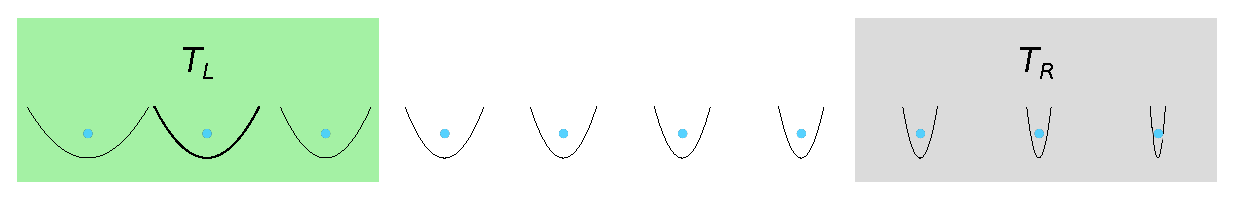
\includegraphics[width=0.9\linewidth]{Figures/Diagram.eps}
    \caption{Schematic representation  of the frequency-graded chain of trapped ions proposed as a thermal rectifier. The left and right ends of the chain are in contact with optical molasses at temperatures $T_L$ and $T_R$ (green and grey boxes respectively). Each ion is in an individual trap. The (angular) frequencies of the traps increase homogeneously from left to right, starting from $\omega_1$ and ending at $\omega_1+\Delta\omega$. The ions interact through the Coulomb force, which is long range, and therefore all the ions interact among them, even distant neighbors. By default  I use 15 ions.}
    \label{fig:Diagram}
\end{figure}

The baths are physically implemented by optical molasses consisting of a pair of counterpropagating Doppler-cooling lasers \cite{Ruiz2014}. The friction and diffusion coefficients for the ions in contact with the baths are given in \cite{Cohen1992,Metcalf2003,Ruiz2014}
%
\begin{align}
  \gamma_n &= -4 \hbar k_{L,R}^2 \left(\frac{I_{L,R}}{I_0}\right)\frac{2\delta_{L,R}/\Gamma}{\left[1 + (2\delta_{L,R}/\Gamma)^2\right]^2},\nonumber\\
  %
  D_n &= \hbar^2 k_{L,R}^2 \left(\frac{I_{L,R}}{I_0}\right) \frac{\Gamma}{1 + (2\delta_{L,R}/\Gamma)^2},\nonumber\\
  n &\in \cal{L},\cal{R},
  \label{eq:chapter5_DopplerCooling}
\end{align}
%
where $k_L$ ($k_R$) and $I_L$ ($I_R$) are the wave vector and intensity of the left (right) laser. $\delta_L$ ($\delta_R$) is the detuning of the left (right) laser with respect to the angular frequency $\omega_0$ of the atomic transition the laser is exciting, and $\Gamma$ is the corresponding natural line width of the  excited state. The expressions in eq. \eqref{eq:chapter5_DopplerCooling} are valid only if the intensities of the lasers are small compared to the saturation intensity $I_0$, $I_{L,R}/I_0\ll 1$. In this bath model, the friction term in eq. \eqref{eq:chapter5_Dynamics} comes from the cooling action of the laser and the white noise force $\xi_n(t)$ corresponds to the random recoil of the ions due to spontaneous emission of photons \cite{Metcalf2003,Cohen1992}. Using the diffusion-dissipation relation $D = \gamma k_B T $ \cite{Chee2010}, the temperatures of the optical molasses baths are given by
%
\begin{equation}
    T_{L,R} = -\frac{\hbar \Gamma}{4 k_B} \frac{1+(2\delta_{L,R}/\Gamma)^2}{(2\delta_{L,R}/\Gamma)},
    \label{eq:chapter5_Doppler}
\end{equation}
%
with $k_B$ being the Boltzmann constant. If the laser intensities are low enough, the temperatures of the baths are controlled by modifying the detunings. When $\delta = \delta_D=-\Gamma / 2$ the optical molasses reach their minimum possible temperature, the Doppler limit $T_{D} = {\hbar \Gamma}/({2k_B})$. Note that away from the Doppler limit the same temperature may be achieved
for two different values of the detuning. These two possibilities imply different couplings (two different pairs of $\gamma$ and $D$ values) and thus different physical effects that will be studied in section \ref{TC}.
%
%
%
%
\section{Calculation of the stationary heat currents\label{sec:chapter5_HeatFlow}}
%
%
The local energy of each site is defined by
%
\begin{equation}
    H_n = \frac{1}{2m} p_n^2 + \frac{1}{2}m\omega_n^2 \left( x_n - x_n^{(0)}\right)^2 +\frac{1}{2}\sum_{l\neq n} V_C(\left|x_n-x_l\right|).
    \label{eq:chapter5_LocalEnergy}
\end{equation}
%
Differentiating $H_n$ with respect to time I find the continuity  equation
%
\begin{equation}
    \dot{H}_n = \frac{p_n}{m}\! \left[ \xi_n(t)-\gamma_n \frac{p_n}{m} \right]\! - \frac{1}{2m}\!\sum_{l\neq n}\frac{\partial V_C (\left|x_n\!-\!x_l\right|)}{\partial x_n}(p_n + p_l).
    \label{eq:chapter5_continuityFirst}
\end{equation}
%
Two different contributions can be distinguished: $j^B_n \equiv \frac{p_n}{m} \left[ \xi_n(t)-\gamma_n \frac{p_n}{m} \right]$, which is the energy flow from the laser reservoir to the ions at the edges of the chain (only for $n\in {\cal L}, {\cal R}$), and $\dot{H}_n^{int} \equiv - \frac{1}{2m}\sum_{l\neq n}\frac{\partial V_C (\left|x_n-x_l\right|)}{\partial x_n}(p_n + p_l)$, which gives the ``internal'' energy flow due to the interactions with the rest of the ions. In the steady state $\expval{\dot{H}_n} = 0$, and therefore
%
\begin{equation}
    \expval{j^B_n} + \expval{\dot{H}_n^{int}} = 0,
    \label{eq:chapter5_continuitySecond}
\end{equation}
%
where $\langle \cdot\!\cdot\!\cdot \rangle$ stands for the expectation value with respect to  the ensemble of noise processes $\bm\xi (t)$ ($\bm\xi$ represents a vector with
components $\xi_n$). Equation \eqref{eq:chapter5_continuitySecond} implies that, in the steady state, the internal rates $\dot{H}_n^{int}$ vanish for the inner ions of the chain because $j^B_n = 0$ for $n\notin {\cal L},{\cal R}$. In chains with nearest-neighbor (NN) interactions,
$\langle\dot{H}_n^{int}\rangle$ simplifies to two compensating and equal-in-magnitude contributions that define the homogeneous heat flux across the chain.
For long-range interactions this is not so and defining the flux is not so straightforward. A formal possibility is to impose
nearest-neighbor interatomic interactions for some atoms in the chain \cite{Chen2015},
but this approach is not realistic in the current system so I define instead the heat currents
for the left and right baths as
%
\begin{align}
  J_L (t)&= \sum_{n\in {\cal L}} \expval{j^B_n},\nonumber\\
  J_R (t)&= \sum_{n\in {\cal R}} \expval{j^B_n},
  \label{eq:chapter5_BathHeatFlows}
\end{align}
%
respectively. These expressions are in general time-dependent. In the steady state $J_{L,{\rm steady}}$ and $J_{R,{\rm steady}}$ should cancel each other since the local energies stabilize and internal energy flows cancel. I will use either $J_{L,{\rm steady}}$ or $J_{R,{\rm steady}}$ to calculate the total energy flow in the chain, always taking the absolute value, i.e., $J \equiv \abs{J_{L,{\rm steady}}}= \abs{J_{R,{\rm steady}}}$. $J$ is defined as $J_\rightarrow$ when the hot bath is on the left
and $J_\leftarrow$ when it is on the right.

To compute the average heat fluxes of the baths $\expval{j^B_n}$ in eq. \eqref{eq:chapter5_BathHeatFlows} I need
the averages $\expval{p_n(t)\xi_n(t)}$. Instead of explicitly averaging $p_n(t)\xi_n(t)$ over different realizations of the white noise, I use Novikov's theorem \cite{Novikov1965,Ma2011,Toral2014}. Novikov's theorem states that the ensemble average (over  the realizations of the noise) of the product of some functional $\phi(t)$, which depends on a set of
$n_{noise}$ Gaussian noises $\xi_i(t)$ with zero mean value, $\expval{\xi_i(t)} = 0$, and the noise itself, is given by
%
\begin{equation}
    \expval{\xi_i(t)\phi(t)} = \sum_{j=1}^{n_{noise}}\int_0^t dt' \expval{\xi_i(t)\xi_j(t')} \expval{\frac{\delta \phi(t)}{\delta\xi_j(t')}},
    \label{eq:chapter5_Novikov_GeneralExpression}
\end{equation}
%
where ${\delta \phi(t)}/{\delta\xi_j(t')}$ is the functional derivative of $\phi(t)$ with respect to the $j$-th component of the noise. Since the noises are independent from each other and $\delta-$correlated,
%
\begin{align}
  \expval{\xi_i(t)\phi(t)} &= 2D_i \overbrace{\int_0^t dt' \delta(t-t') \expval{\frac{\delta \phi(t)}{\delta\xi_i(t')}}}^{= \frac{1}{2} \lim_{t'\to t^-} \expval{\frac{\delta \phi(t)}{\delta\xi_i(t')}} }\nonumber\\
  &=D_i \lim_{t'\to t^-} \expval{ \frac{\delta \phi(t)}{\delta\xi_i(t')} }.
  \label{eq:chapter5_Novikov_WhiteIndependentNoise}
\end{align}
%
The $1/2$ factor from the integral in eq. \eqref{eq:chapter5_Novikov_WhiteIndependentNoise} comes from the assumption that the Dirac delta function is the limit of even correlation functions when the correlation time goes to 0. The notation $\lim_{t'\to t^-}$ stands for the limit when $t'$ goes to $t$ from below ($t'<t$). To evaluate the functional derivatives of the position $x_n(t)$ and momentum $p_n(t)$ coordinates with respect to the white noises, I integrate eq. \eqref{eq:chapter5_Dynamics} to have its formal solution as a functional depending on the white Gaussian noises $\xi_n(t)$,
%
\begin{align}
  x_n(t) &= x_n(0) +  \frac{1}{m}\int_0^t ds\; p_n(s) ,\nonumber\\
  p_n(t) &= p_n(0) + \int_0^t ds\; \left[ -\frac{\partial H}{\partial x_n}(s) - \frac{\gamma_n}{m}p_n(s) + \xi_n(s)\right].
  \label{eq:chapter5_FormalSolution}
\end{align}
%
Taking the functional derivatives of eq. \eqref{eq:chapter5_FormalSolution} I get for $t'<t$
%
\begin{align}
  \frac{\delta x_n(t)}{\delta \xi_m(t')} &= \frac{1}{m}\int_{t'}^{t} ds\; \frac{\delta p_n(s)}{\delta \xi_m(t')},\nonumber
  %
  \\
  %
  \frac{\delta p_n(t)}{\delta \xi_m(t')} &= \delta_{nm} -\int_{t'}^{t} ds\;\frac{\delta}{\delta \xi_m(t')}\left[\frac{\partial H}{\partial x_n}(s) + \frac{\gamma_n}{m}p_n(s) \right].
  \label{eq:chapter5_functional_derivatives}
\end{align}
%
The integration limits in eq. \eqref{eq:chapter5_functional_derivatives} go from $t'$ to $t$ since the functional derivatives are $0$ when $s<t'$, because the values of the noise in the future cannot affect a signal in the present, which would break causality. I have also used that $\frac{\delta \xi_n(t)}{\delta \xi_m(t')} = \delta_{nm}\delta(t-t')$. Taking the limit $t'\to t^-$ in eq. \eqref{eq:chapter5_FormalSolution} I obtain the values of the functional derivatives of $x_n$ and $p_n$, $ \lim_{t'\to t^-} \delta x_n(t)/\delta \xi_m(t') = 0$ and $\lim_{t'\to t^-} \delta p_n(t)/\delta \xi_m(t') = \delta_{nm}$ ($\delta_{nm}$ is the usual Kronecker delta). Thus I have $\expval{x_n(t) \xi_m(t)} = 0$ and $\expval{p_n(t) \xi_m(t)} = \delta_{nm}D_m$, which gives for the heat flow from the baths
%
\begin{equation}
    \expval{j^B_n} = \frac{1}{m} \left[ D_n-\gamma_n \frac{\expval{p_n^2}}{m} \right].
    \label{eq:chapter5_BathHeatFlowNovikov}
\end{equation}
%
In all simulations I check that $|J_{L,{\rm steady}}|=|J_{R,{\rm steady}}|$ within the numerical tolerance of the computer. To measure the asymmetry of the heat currents I use the rectification factor $R$ defined as
%
\begin{equation}
    R = \frac{ J_\rightarrow - J_\leftarrow}{max(J_\rightarrow,J_\leftarrow)}.
    \label{eq:chapter5_R_Factor}
\end{equation}
%
$R$ may go from $-1$ to $1$ (In the figures I depict it in \% between -100\% and 100\%). If there is no rectification $J_\rightarrow = J_\leftarrow $ and $R=0$. For perfect rectification in the right (left) direction, $J_\rightarrow \gg J_\leftarrow$ ($J_\rightarrow \ll J_\leftarrow$), and $R = 1$ ($R = -1$).
Notice that other  definitions of rectification factors exist in many works
on asymmetric heat transfer so comparisons should be done with care.
%

This model does not show the antithermodynamical behavior  observed in other models
\cite{De-Chiara2018,Levy2014}, and heat is found to flow in all cases from the hot to the
cold bath.
%
%
%
\subsection{Algebraic, small-oscillations approach to calculate the steady state\label{sec:chapter5_steadyState}}
%
%
%
%
To find the temperature profiles and heat currents in the steady state the usual approach is to solve the SDE system in eq. \eqref{eq:chapter5_Dynamics} up to long times  and for many realizations of the white noises $\bm\xi (t)$. In that way, the ensemble averages $\expval{p_n(t \to \infty)^2}$, necessary for both the temperature profiles and heat currents, are computed. This standard route implies a heavy computational effort, in particular  when I want to study the heat transport for several bath configurations, frequency increments and chain parameters. It is possible to circumvent this difficulty and find ensemble averages like $\expval{x_n x_m}$, $\expval{x_n p_m}$, $\expval{p_n p_m}$ (second order moments) without integrating any SDE \cite{Sarkka2019,Rieder1967,Casher1971}. The idea is to impose the condition ${d\expval{\cdot\cdot\cdot}}/{dt} = 0$ for all the second order moments and linearize the dynamical equations of the system around equilibrium.
A system of linear algebraic equations for the moments results, that can be easily solved without solving the SDE many times.
% to solve a system of linear algebraic equations. I will analyze the validity of the linearized approximation in the following section.

\begin{figure}
  \center
  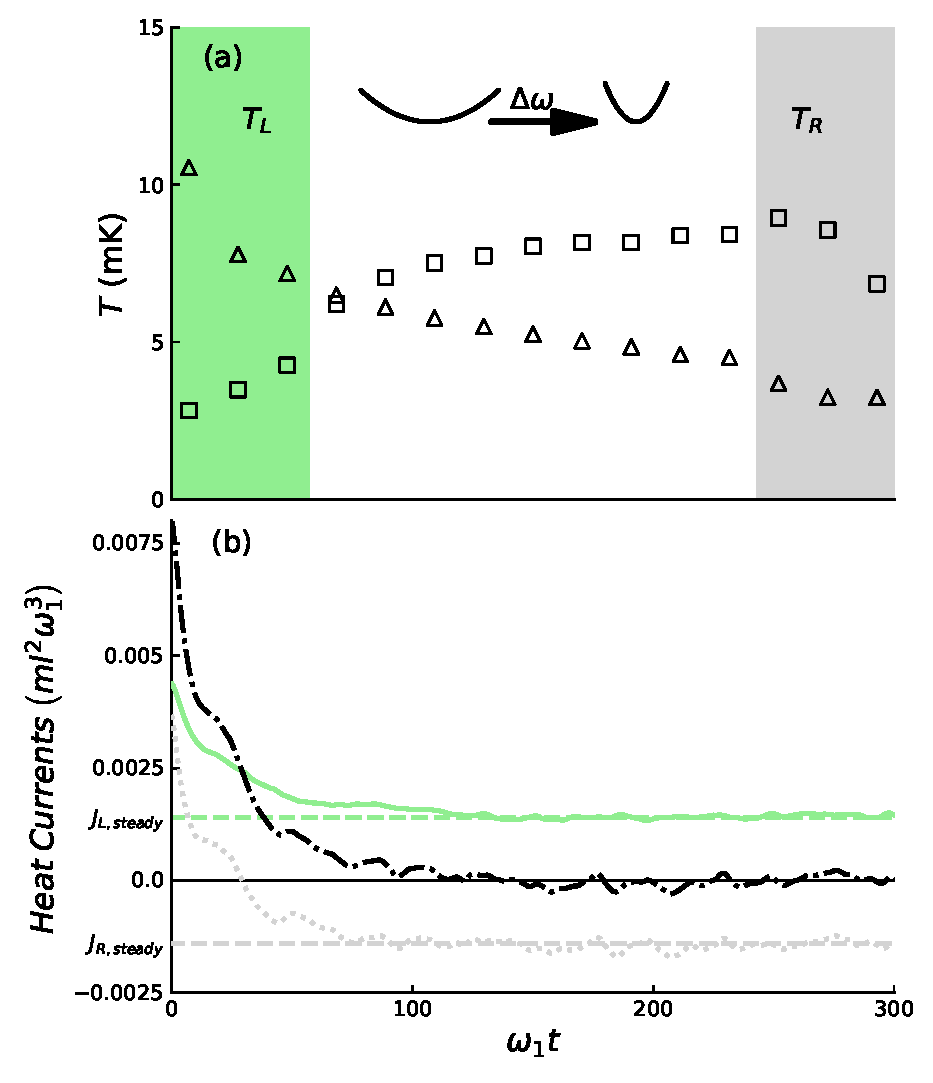
\includegraphics[width=0.85\linewidth]{Figures/24Mg_Temperature_Profiles_And_Evolution.eps}
  \caption{(a) Temperatures of the ions in the stationary state for a graded chain with the parameters described in section \ref{Results_A}. The temperature profiles found with the algebraic method (eq. \eqref{eq:chapter5_SteadyStateEquation}) are indistinguishable from the ones found solving the Langevin equation (eq. \eqref{eq:chapter5_Dynamics}). Empty triangles (squares) correspond to $T_L = T_H$ ($T_L = T_C$) and $T_R = T_C$ ($T_R = T_H$). (b) Heat currents  as a function of time for $T_L = T_H$ and $T_R = T_C$, see eq. (\ref{eq:chapter5_BathHeatFlows}): $J_L(t)$ (solid green line) from the left reservoir into the chain;$J_R(t)$ (dotted grey line) from the right reservoir into the chain (negative except at very short times); $J_L(t)+J_R(t)$ (dotted-dashed black line), which must go to zero in the steady state. The three lines tend to stationary values marked by horizontal lines. Parameters: $\omega_1 = 2\pi \times 50$ kHz, $a=50\, \mu$m,  $\delta_H = -0.02 \, \Gamma$, and $\delta_C = -0.1 \, \Gamma$, which gives temperatures $T_H \approx 12$ mK and $T_C \approx 3$ mK. $\Delta\omega = 0.5 \, \omega_1$. In all figures $\Gamma = 2\pi \times 41.3$ MHz.}
  \label{fig:Temperature_Profiles_Magnesium}
\end{figure}

To linearize the SDE in eq. \eqref{eq:chapter5_Dynamics} I approximate the potential energy of the Hamiltonian in eq. \eqref{eq:chapter5_ChainHamiltonian}, $V(\bm{x}) = V_{int}(\bm{x}) + m\;\sum_n \omega_n^2 (x_n-x_n^{(0)})^2/2$, by its harmonic approximation around the equilibrium positions $\bm{x}^{eq}$, defined by  $\frac{\partial V(\bm{x})}{\partial\bm{x}}\Big|_{\bm{x}=\bm{x}^{eq}} = 0$. The approximate potential (ignoring the zero-point energy) is
%
\begin{equation}
    V(\bm{x})\approx  \frac{1}{2} \sum_{n,m} K_{nm} (x_n-x_n^{eq})(x_m-x_m^{eq}),
\end{equation}
%
with $K_{nm} = \frac{\partial^2 V(\bm{x})}{\partial x_n \partial x_m}\Big|_{\bm{x}=\bm{x}^{eq}}$ being the Hessian matrix entries of $V(\bm{x})$ around the equilibrium configuration \cite{James1998}
%
\begin{equation}
    K_{nm} =
    \begin{cases}
        m \omega_n^2 + 2 \left(\frac{q^2}{4\pi\varepsilon_0}\right) \sum_{l \neq n  }\frac{1}{\left|x_n^{eq}-x_l^{eq}\right|^3} & \text{if  } n=m\\

         - 2 \left(\frac{q^2}{4\pi\varepsilon_0}\right) \frac{1}{\left|x_n^{eq}-x_m^{eq}\right|^3} & \text{if  } n \neq m
    \end{cases}.
\end{equation}
%
Note that this approximation does not modify the two main features of the system, namely asymmetry and long-range interactions, which are manifest in the asymmetric distribution of $\omega_n$ and the non-zero off-diagonal elements of the $K$ matrix, respectively. In the following I will use $y_n=x_n-x_n^{eq}$ to simplify the notation. The linearized dynamics around the equilibrium positions are given by
%
\begin{align}
  \dot{y}_n &= \frac{1}{m}p_n,\nonumber\\
  \dot{p}_n &= -\sum_{l}K_{nl}y_l- \frac{\gamma_n}{m}p_n + \xi_n(t).
  \label{eq:chapter5_DynamicsHarmonic}
\end{align}
%
Now, I set ${d\expval{\cdot\!\cdot\!\cdot}}/{dt} = 0$ for all the moments. Using eq. \eqref{eq:chapter5_DynamicsHarmonic} and applying Novikov's theorem I find

%
\begin{align}
  \expval{p_n p_l} - \gamma_l\expval{y_n p_l} - \sum_m K_{lm}\expval{y_n y_m} &= 0,\nonumber\\
  \sum_{m}\left[ K_{nm}\expval{y_m p_l} + K_{lm}\expval{y_m p_n} \right] + \frac{1}{m}\left( \gamma_l + \gamma_n \right)\expval{p_n p_l} &= 2 \delta_{nl} D_n.
  \label{eq:chapter5_SteadyStateEquation}
\end{align}
%
The system \eqref{eq:chapter5_SteadyStateEquation} is linear in the second order moments so it can be solved numerically to find the steady-state values of the moments. Besides eq. \eqref{eq:chapter5_SteadyStateEquation} I have that $\expval{y_n p_l} = - \expval{y_l p_n}$, which follows from eq. \eqref{eq:chapter5_DynamicsHarmonic} and $d\expval{y_n y_m}/dt = 0$. Since there are $\frac{1}{2}N(N-1)$ independent $\expval{y_n p_l}$ moments, I choose the ones with $n<l$. Similarly, the moments $\expval{y_n y_l}$ and $\expval{p_n p_l}$ contribute with $\frac{1}{2}N(N+1)$ independent variables each and I choose the ones with $n\leq m$. Thus there are in total $\frac{1}{2}N(3N+1)$ independent moments that can be arranged in the vector
%
\begin{align}
    \bm\eta = \Big[ &\expval{y_1 y_1},\expval{y_1 y_2},...,\expval{y_N y_N},\nonumber\\
    &\expval{p_1 p_1},\expval{p_1 p_2},...,\expval{p_N p_N},\nonumber\\
    &\expval{y_1 p_2},\expval{y_1 p_3},...,\expval{y_{N-1} p_N}\Big]^T.
    \label{eq:chapter5_CovariancesVector}
\end{align}
%
There are the same number of independent equations
%in eq. \eqref{eq:chapter5_SteadyStateEquation}
as independent moments: $N^2$
equations correspond to the first line in eq.  \eqref{eq:chapter5_SteadyStateEquation}, and $\frac{1}{2}N(N+1)$ equations
to the second line because of the symmetry with respect to $n,l$. The system of equations \eqref{eq:chapter5_SteadyStateEquation} may be compactly written as $\mathbf{A}\boldsymbol\eta = \mathbf{B}$, where $\mathbf{A}$ and $\mathbf{B}$ are a $\frac{1}{2}N(3N+1)$ square matrix and vector.

\section{Numerical Results\label{sec:chapter5_NumericalResults}}


I now display the results of the simulations. To find the temperature profiles and the currents in the steady state I use the algebraic method described in section \ref{sec:chapter5_steadyState}. I also check that the results coincide with those by solving eq. \eqref{eq:chapter5_Dynamics} for many different realizations of the noise forces $\bm\xi (t)$ and averaging. The code for all the numerical simulations has been written in the language \textit{Julia} \cite{Bezanson2012,Bezanson2017}. In particular, to solve the Langevin equation, I used \textit{Julia}'s package \textit{DifferentialEquations.jl} \cite{Rackauckas2017}.

To model the baths and the chain I use atomic data taken from ion trap experiments \cite{Leupold2015,Lo2015}. I consider 15 $^{24}$Mg$^+$ ions in all figures except in fig. \ref{fig:N_Dependence}. Only the three leftmost and three rightmost ions interact with Doppler cooling lasers. The Doppler cooling lasers excite the transition $3s^2S_{1/2}\rightarrow 3p^2P_{1/2}$, with angular frequency $\omega_0 = 2 \pi \times 1069$ THz and excited state line width $\Gamma = 2\pi \times 41.3$ MHz \cite{Ruiz2014}. For this ionic species and atomic transition the Doppler limit is $T_D = 1$ mK.
%I use typical trap frequencies of the order of MegaHertzs and intertrap spacings of a few tens of $\mu$m.
The intensities of the laser beams are small compared to the saturation intensity $I_0$ so that eq. \eqref{eq:chapter5_DopplerCooling} holds. I take $I_n/I_0 = 0.08$ for the ions  in the laser beams, whereas  $I_n=0$ for the rest.

The temperatures $T_L,\,T_R$ of the left and right laser baths are controlled with their detunings $\delta_L,\,\delta_R$ with respect to the atomic transition. I fix two values for the detunings, $\delta_H$ and $\delta_C$, such that $T_H>T_C$ (hot and cold baths, also source and drain) and I define $J_\rightarrow$ ($J_\leftarrow$) as the stationary heat current in the chain when $T_L = T_H$ and $T_R = T_C$ ($T_L = T_C$ and $T_R = T_H$).

Except in section \ref{GS} I consider a graded frequency profile.
%In the graded chain the frequency increases by $\frac{\Delta\omega}{N-1}$ from one trap to the next.
If the frequency of the leftmost trap is $\omega_1$, the frequency of the $n$th trap will be $\omega_n = \omega_1 +\Delta\omega\frac{n-1}{N-1}$ up to $\omega_1 +\Delta\omega$ for the rightmost trap. In
section \ref{GS}, I compare the graded chain to a segmented chain, where the left half of the chain has trapping frequencies $\omega_1$ while the other half has $\omega_1 +\Delta\omega$.


\subsection{Evolution to steady state \label{Results_A}}

\begin{figure}
  \center
  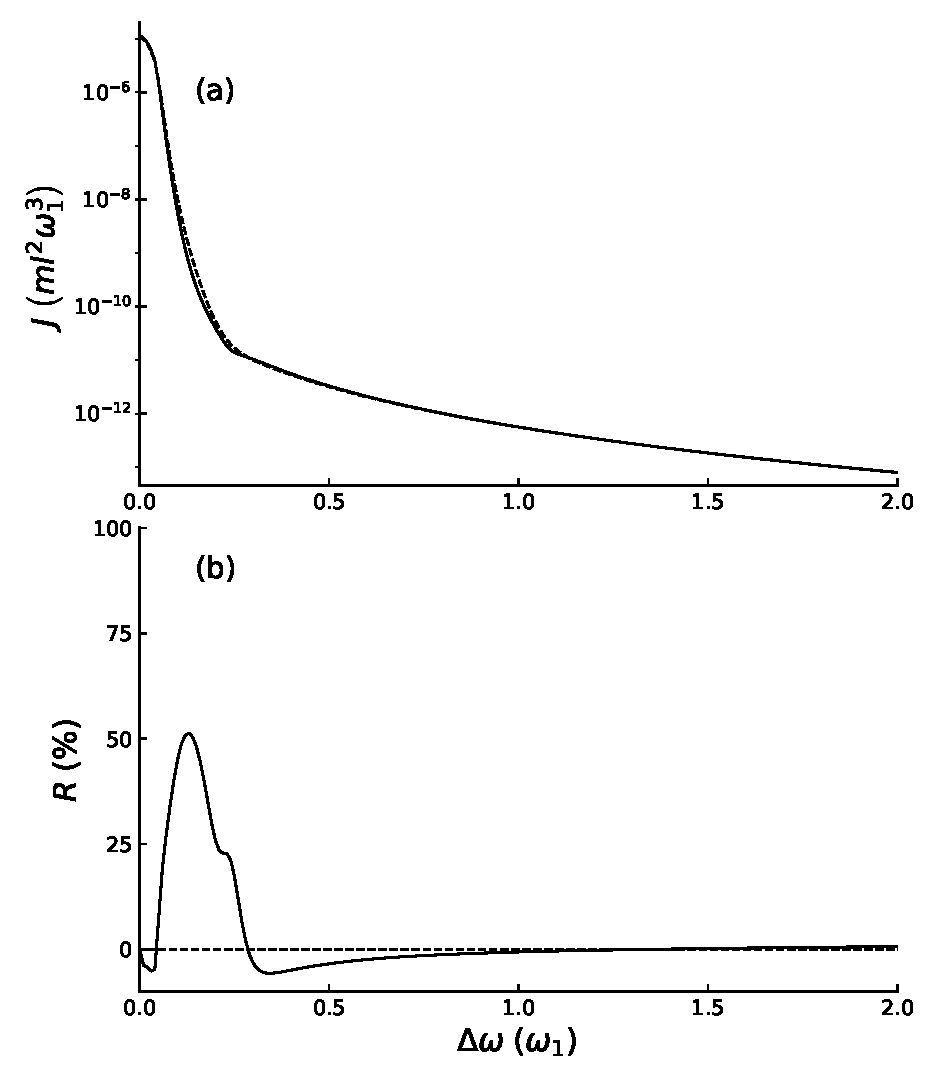
\includegraphics[width=0.85\linewidth]{Figures/Graded_24Mg_FluxAndRectification_VS_FreqGradient.eps}
  \caption{Graded chain of $N=15$ $^{24}$Mg$^+$ ions. (a) Stationary fluxes for different frequency increments: $J_\rightarrow$   (for $T_L = T_H$ and $T_R = T_C$, dashed line); $J_\leftarrow$ (for $T_L = T_C$ and $T_R = T_H$, solid line) (b) Rectification factor. Parameters: $\omega_1 = 2 \pi \times 1$ MHz, $l = 5.25\;\mu$m, $a = 4.76\, l$ ($25\,\mu$m), $\delta_H = -0.02 \,\Gamma$, and $\delta_C = -0.1 \, \Gamma$.}
  \label{fig:RFG}
\end{figure}

To compare the results by solving eq. \eqref{eq:chapter5_Dynamics} and averaging and those from the algebraic method, I simulated a frequency graded chain with a trapping frequency $\omega_1 = 2\pi \times 50$ kHz for the leftmost ion, see fig. \ref{fig:Temperature_Profiles_Magnesium}.  The number of ions interacting with the laser beams (three on each bath) is consistent with the lattice constant and typical waists of Gaussian laser beams \cite{Leupold2015,Lo2015}. To set the trap distance I fix first the characteristic length  $l =  \left(\frac{q^2}{4\pi\varepsilon_0}\frac{1}{m\omega_1^2}\right)^{1/3}$ as the distance for which the Coulomb repulsion of two ions equals the trap  potential energy for an ion at a distance
$l$ away from the center of its trap.
If $a<l$, the Coulomb repulsion of the ions is stronger than the trap confinement which makes the ions jump from their traps. With the parameters used in this section I have $l = 38.7\,\mu$m and set $a = 1.29 \,l=50\,\mu$m. The detunings of the \textit{hot} and \textit{cold} lasers are $\delta_H = -0.02 \, \Gamma$, and $\delta_C = -0.1 \, \Gamma$ which gives temperatures $T_H \approx 12$ mK and $T_C \approx 3$ mK. I fix the value $\Delta\omega = 0.5 \, \omega_1$ for the frequency increment.

The results of the two methods are in very good agreement. In the scale of fig. \ref{fig:Temperature_Profiles_Magnesium} (a)
the calculated local temperatures are undistinguishable. In the calculation based on solving the dynamics I had to integrate eq. \eqref{eq:chapter5_Dynamics} for $N_{trials} = 1000$ realizations of white noise $\bm{\xi}(t)$. The method based on the system of moments
shortened the calculation time with respect to the dynamical trajectories   by a factor of $1/700$. In fact, the time gain is even more important because
the dynamical method requires further processing, performing a time averaging to compute the stationary flux in addition to noise averaging, see fig.  \ref{fig:Temperature_Profiles_Magnesium} (b).


Additionally, the relaxation to the steady state slows down when the frequencies of the traps increase since the deterministic part of the Langevin equation dominates the dynamics over the stochastic part, entering an under-damped regime. In contrast, this increase does not affect the
algebraic method.
%%%%%%%%%%%%%%%%%%%%
\begin{figure}
  \center
  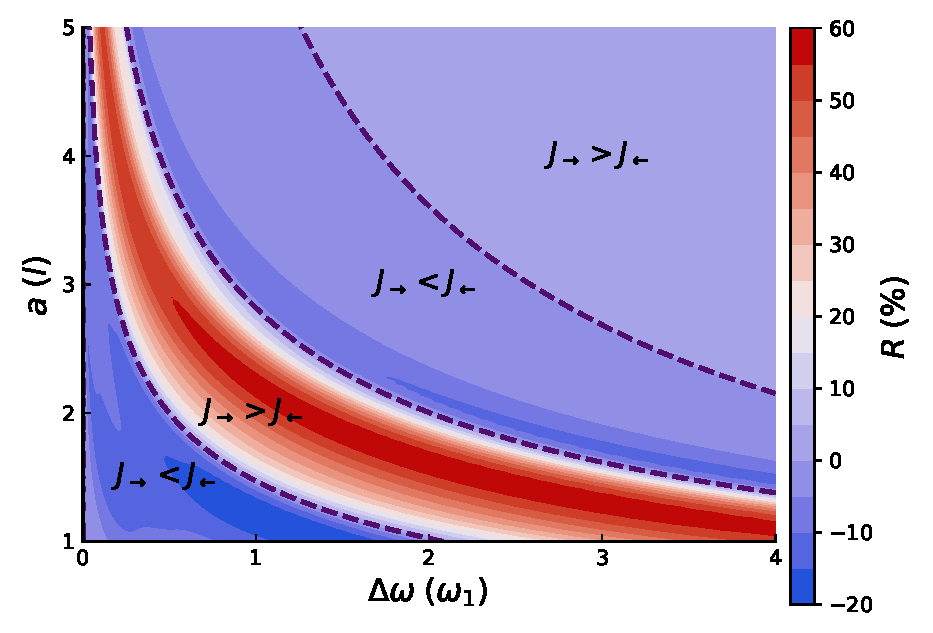
\includegraphics[width=0.85\linewidth]{Figures/Graded_24Mg_Rectification_VS_Gradient_and_lattConstant.eps}
  \caption{ Rectification factor in a graded chain of $N=15$ $^{24}$Mg$^+$ ions for different trap distances and frequency increment. The dashed lines are for $R = 0$ and delimit the regions $J_\rightarrow > J_\leftarrow$ and $J_\rightarrow < J_\leftarrow$. The parameters  are $\omega_1 = 2 \pi \times 1$ MHz, $l = 5.25\,\mu$m, $\delta_H = -0.02 \,\Gamma$, and $\delta_C = -0.1 \, \Gamma$.}
  \label{fig:Graded_24Mg_Rectification_VS_Gradient_and_lattConstant}
\end{figure}
%
%
%
%
\subsection{Rectification in frequency graded chains \label{GradedChains}}
%
%
\begin{figure}
  \center
  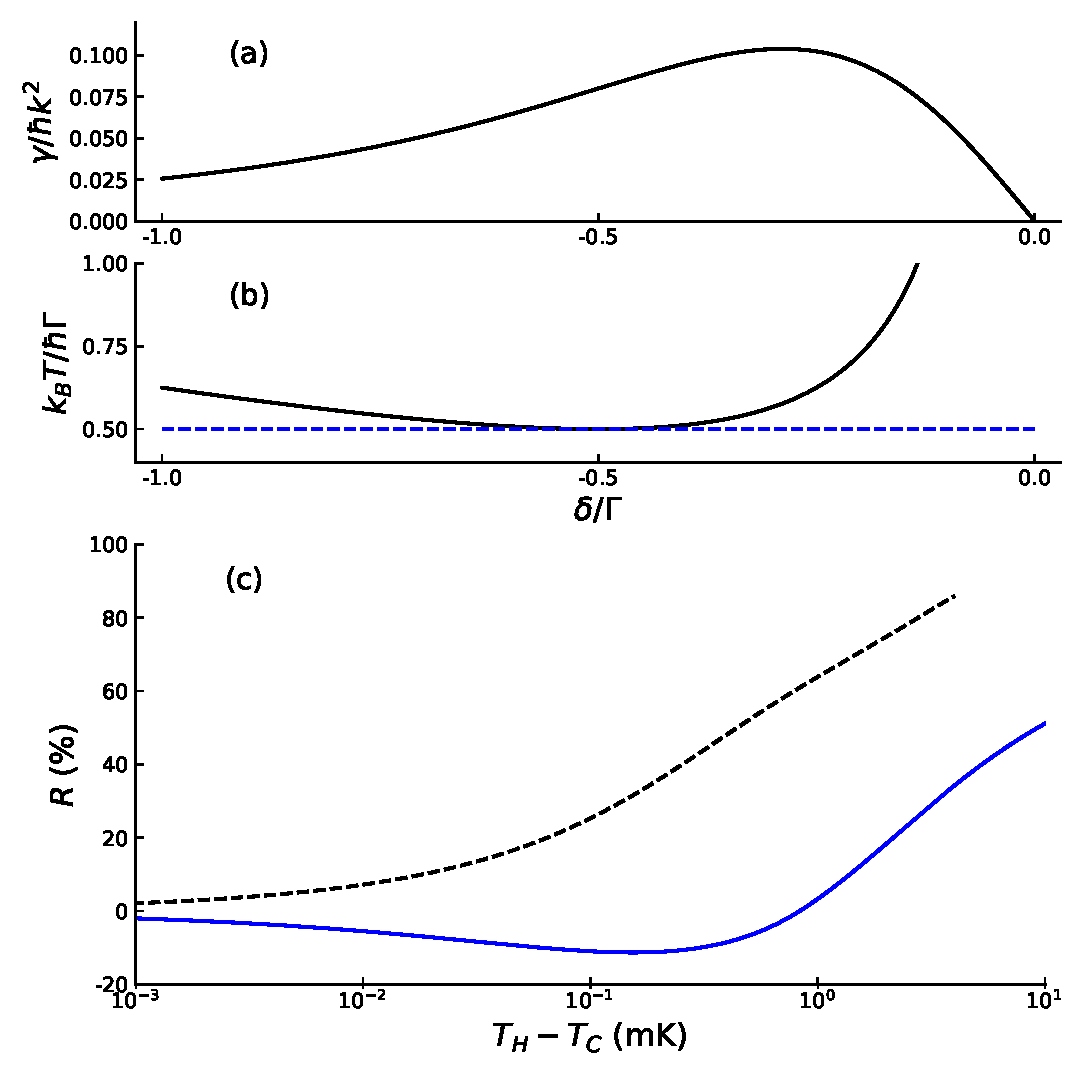
\includegraphics[width=0.85\linewidth]{Figures/R_as_function_of_TemperatureBias.eps}
  \caption{ (a) Friction coefficient defined in eq. \eqref{eq:chapter5_DopplerCooling}. (b) Bath temperature defined in eq. \eqref{eq:chapter5_Doppler}. (c) Rectification as a function of the temperature difference between the hot and cold baths $T_H -T_C$ for $\delta_H$ below (dashed black line) and above (solid blue line) the Doppler limit, and $\delta_C=\delta_D$ (Doppler limit). Parameters: $\omega_1 = 2 \pi \times 1$ MHz, $\Delta \omega = 0.15 \, \omega_1$, $l = 5.25\,\mu$m, $a = 4.76 \, l$.}
  \label{fig:RD}
\end{figure}
%
In this subsection I demonstrate rectification for the frequency graded chain. I  used the method described in section \ref{sec:chapter5_steadyState} for $^{24}$Mg$^+$ ions with the same parameters for the baths used before. I fix the trapping frequency of the leftmost trap to $\omega_1 = 2\pi \times 1$ MHz, and a trap spacing $a = 4.76\, l$ ($25\,\mu$m) (the  characteristic length is $l = 5.25\,\mu$m). Figure \ref{fig:RFG} depicts  the results with these parameters in a graded chain. Figure \ref{fig:RFG} (a) shows that both
$J_\rightarrow$ and $J_\leftarrow$
% the right-going flux (dashed line) and the left-going flux (solid line)
decrease rapidly as the frequency increment  is increased.
%In fig. \ref{fig:Graded_24Mg_FluxAndRectification_VS_FreqGradient} I see that
The rectification reaches its maximum value for a frequency difference of $\Delta\omega \approx 0.1 \omega_1$. The fluxes cross so there are some points where the rectification is exactly zero, besides the trivial one at $\Delta\omega = 0$, at $\Delta\omega = 0.05\,\omega_1,\;0.3\,\omega_1,\;1.3\,\omega_1$. At these points the direction of rectification reverses, presumably as a consequence of the changes in the match/mismatch of the temperature dependent local power spectra.
The change of rectification direction occurs for all the choices of parameters, as displayed in fig. \ref{fig:Graded_24Mg_Rectification_VS_Gradient_and_lattConstant}. Figure \ref{fig:Graded_24Mg_Rectification_VS_Gradient_and_lattConstant} gives the rectification factor for different trap distances and frequency increments.  $0$-rectification curves separate regions with different rectification direction. The second region in fig. \ref{fig:Graded_24Mg_Rectification_VS_Gradient_and_lattConstant} (starting from the left) would be the most interesting one to build a thermal diode, since rectification reaches its largest values there.

{For small values of $\Delta \omega$ there is little asymmetry in the chain and therefore modest rectification is expected whereas a very large $\Delta \omega$ implies very high trapping frequencies on the right implying a too strong confinement and vanishing interactions. This bottleneck reduces the fluxes in both directions and  the rectification. However, since $\Delta \omega$ is controllable,
and the range of values of $\Delta \omega$ for which rectification is larger can be also controlled with the intertrap distance $a$, see fig. \ref{fig:Graded_24Mg_Rectification_VS_Gradient_and_lattConstant},
the existence of a rectification window
does not imply a major limitation.}

\begin{figure}
  \center
  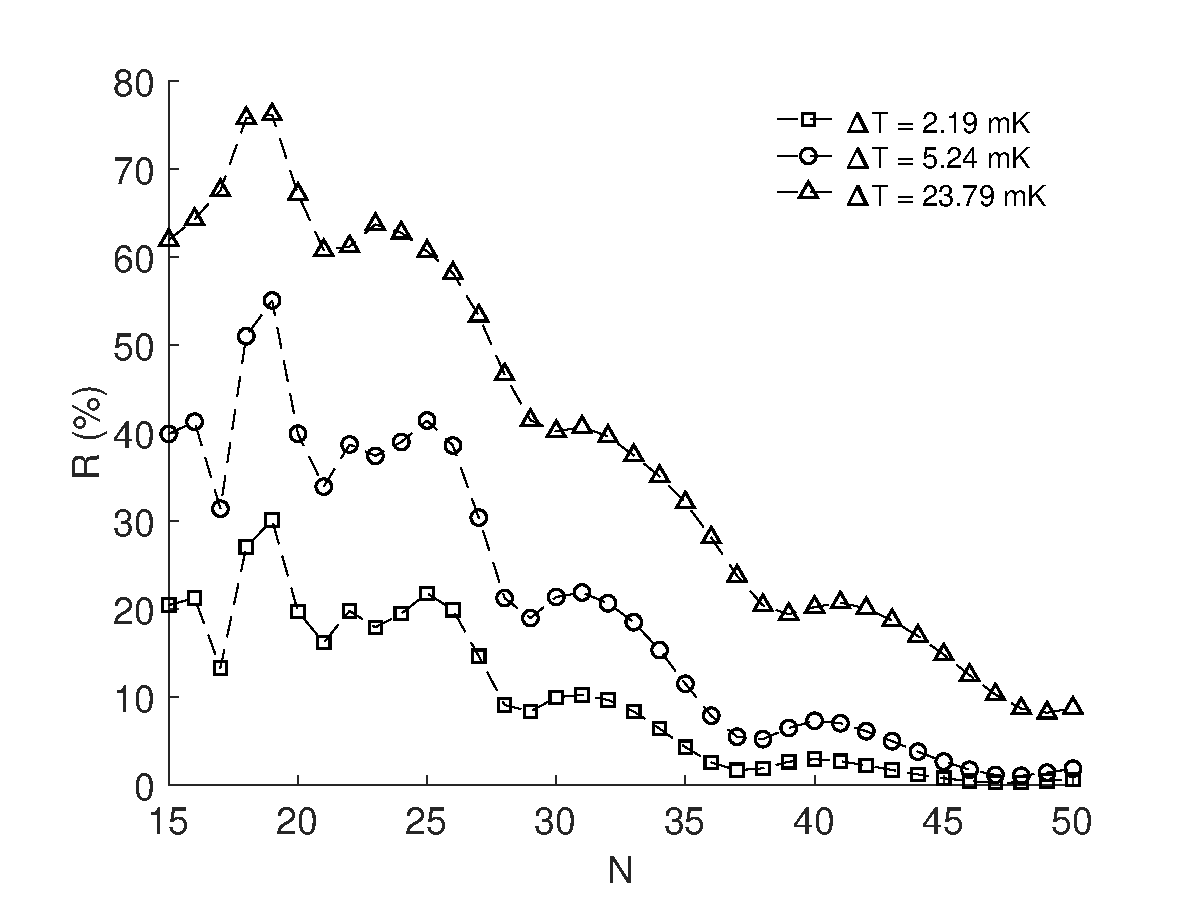
\includegraphics[width=0.85\linewidth]{Figures/Changing_N.eps}
  \caption{Rectification factor for different bath temperature differences $\Delta T$ as the number of ions is increased. The detuning of the cold bath laser is set to the Doppler limit $\delta_C = - \Gamma / 2$. $\omega_1 = 2 \pi \times 1$ MHz, $\Delta \omega = 0.15 \, \omega_1$, $l = 5.25\,\mu$m, $a = 4.76 \, l$.}
  \label{fig:N_Dependence}
\end{figure}
%
%
\subsection{Same bath temperatures, different bath couplings\label{TC}}
%
%
As already mentioned (below eq. \eqref{eq:chapter5_Doppler}), above and below the detuning  $\delta_D=-\Gamma/2$ corresponding to the  Doppler limit temperature, the optical molasses allow for
two different couplings (two pairs of friction and diffusion coefficients in eq. (\ref{eq:chapter5_DopplerCooling})) between the ions and the laser corresponding to the same bath temperature.
This duality may be seen explicitly in fig. \ref{fig:RD}. Specifically fig. \ref{fig:RD} (a) depicts the variation of the friction coefficient for values of $\delta$ around $\delta_R$,  and fig. \ref{fig:RD} (b) the corresponding temperatures.
Interestingly, the different couplings imply different rectification factors.
% To check if this requirement is fulfilled I have calculated the rectification factor for different temperatures in the baths.
If I set $\delta_C = \delta_D=-\Gamma / 2$,  i.e., the cold bath is cooled to the Doppler limit, $\delta_H$ can be chosen to be below or above $\delta_D$ for the same temperature $T_H$. The corresponding rectification factors for the two choices
are shown in  fig. \ref{fig:RD} (c),
%I see that it is possible to achieve comparable rectifications for smaller temperature differences when $\delta_H<\delta_D$.
%Note that since the effective laser temperatures depend on the linewidth $\Gamma$ of the atomic transition, the range of temperatures that can be reached is limited to the mK. Although other works have shown rectification in temperatures of the order of 100 K \cite{Elzouka2017}, the nature of the rectification mechanism and the physical system are very different. Here I have considered an atomic system, instead of a macroscopic one, where the temperatures are intrinsically low.
which
demonstrates that significant rectification can be achieved by choosing $\delta_H<\delta_D$ for temperature increments that
are smaller than or of the order of $T_C=T_D$, for example $R\approx 20\%$ for $\Delta T=0.1 T_C$, or $R\approx 60\%$
for $\Delta T= T_C$.  Finding good rectification at low (relative) temperature differences is considered to be one on the challenges
in asymmetric heat transport research \cite{Zhang2015}.

%
%
%
\subsection{Dependence with number of ions\label{IN}}
%
Keeping in mind that scaling the frequency-graded ion chain  to a large numbers of ions is not a realistic option in this setting,
it is nevertheless important to
study the dependence with ion number from small to moderate numbers.  In fig. \ref{fig:N_Dependence} I observe an overall trend in which the rectification decreases with the number of ions in the chain (while it increases with temperature bias $\Delta T$ in the studied range). This effect is easy to understand, as increasing $N$
while keeping the total variation of the trapping frequency $\Delta \omega$ constant, the frequency gradient  decreases. This
lowers  the  asymmetry in the chain and the rectification factor. Oscillations with $N$ superimposed to the global trend are more visible for smaller $N$ giving  an optimal value at $N=19$.

\subsection{Graded versus segmented\label{GS}}
%
I have also compared the performance of the graded thermal diode and a segmented version in which the left half of the chain is trapped with frequency $\omega_1$ and the right half (including the middle ion) with $\omega_1+\Delta \omega$. Even though the optimal rectification  in fig. \ref{fig:GS} (a)  for the segmented chain is larger than for the graded chain, the fact that the fluxes are generally much larger for the graded chain, see fig. \ref{fig:GS} (b), makes the graded chain more interesting for applications.



\begin{figure}
  \center
  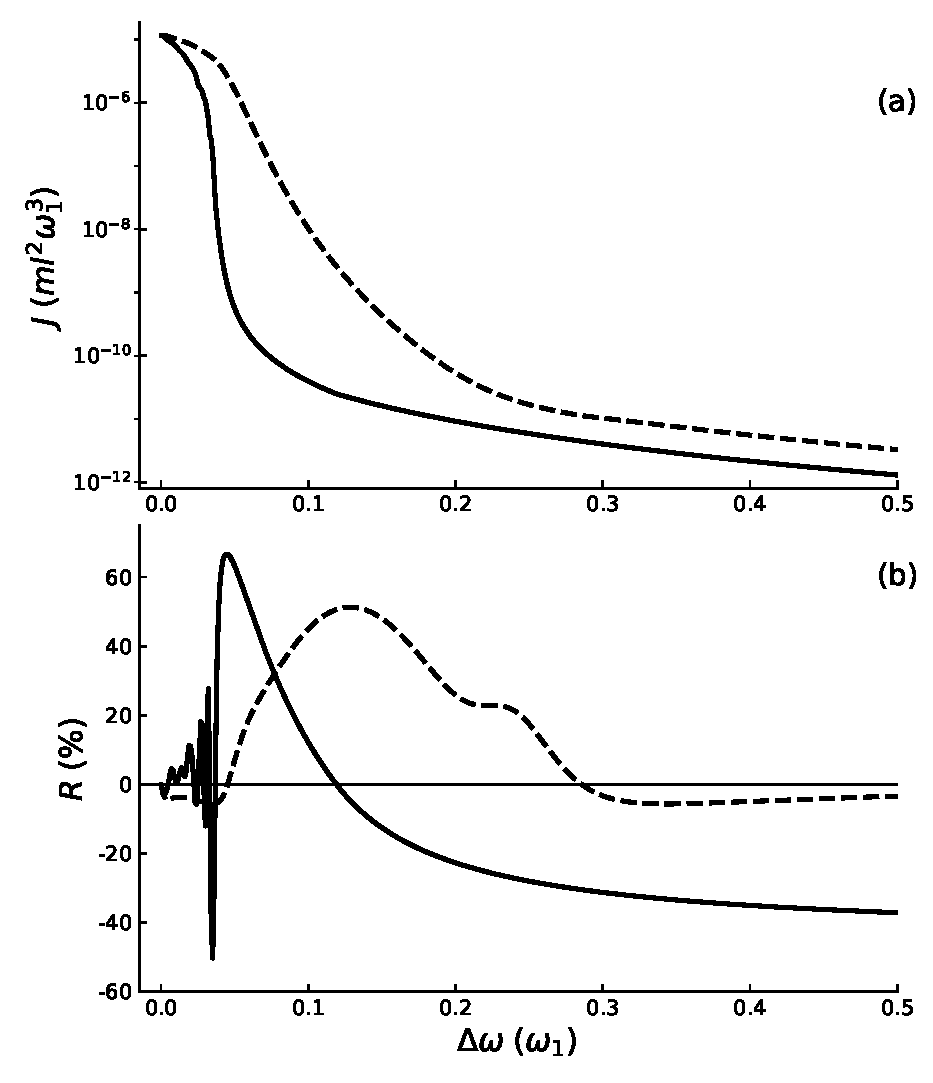
\includegraphics[width=0.85\linewidth]{Figures/24Mg_Comparacion_Graded_AND_Segmented.eps}
  \caption{Comparison of graded and segmented chains with $N=15$ $^{24}$Mg$^+$ ions. (a) Maximum
  of $J_\rightarrow$ and $J_\leftarrow$
   for the graded and segmented chain for different frequency increments. (b) Rectification factor: graded chain (dashed lines); segmented chain (solid lines). Parameters: $\omega_1 = 2 \pi \times 1$ MHz, $l = 5.25\,\mu$m, $a = 4.76 \, l$, $\delta_H = -0.02 \, \Gamma$, and $\delta_C = -0.1 \, \Gamma$.}
  \label{fig:GS}
\end{figure}

\section{Discussion\label{sec:chapter5_Discussion}}
%
In this chapter I have numerically demonstrated heat rectification in a chain of ions trapped in individual microtraps with graded frequencies, connected at both ends to thermal baths
created by optical molasses. An alternative to implement a graded
frequency profile in the lab
could be combining a collective Paul trap for all the ions with on-site dipolar laser forces \cite{Freitas2015,Enderlein2012,Bermudez2013,Schneider2010}.

A goal of this chapter is to connect two communities, ion trappers and
researchers on heat-rectification models. The results found are encouraging and demonstrate the potential of a trapped-ion platform to experimentally investigate heat rectification schemes. Trapped ions are quite interesting to this end because  they are highly controllable,  and may easily adopt several features to enhance rectification, such as
the ones explored here (long-range interactions and an asymmetrical gradation),
or others such as time-dependent forces \cite{Li2012,Riera-Campeny2018}, or different non-linearities in on-site forces.
The limitations and application domain should also be clear,  the proposed platform is circumscribed to cold temperatures of the order of hundreds of $\mu$K to mK achieved by Doppler cooling.
In this sense it is not aimed at competing  with (it is rather complementary to)
proposals for which experiments  \cite{Chang2006,Leitner2013,Kobayashi2009,Elzouka2017} or simulations \cite{Zhang2015,Ma2018,Reid2019}
demonstrate thermal rectification
at room temperature or for hundreds of K.
Also, the number of ions should realistically be kept small so the proposed ion chain
is not aimed at achieving a macroscopic diode length, but at playing a role in thermal diode research
and in the context of ion-trapped based quantum technologies.

Methodologically, the calculation of the steady state has been performed with an algebraic approach much faster than
the time-consuming integration and averaging over noise and time of the dynamical equations.
The algebraic approach linearizes the forces around equilibrium positions which, in this system and for the realistic parameters considered  is well justified and tested numerically.
The results found provide additional evidence that simple linear models may  rectify heat flow \cite{Pereira2017}.  I  underline that this linear
model is, arguably,  even simpler than some linear ``minimalist, toy models'' in \cite{Pereira2017} that showed rectification (the on-site forces are already linear from the start and the temperature dependence of explicit model parameters is only in the coefficients of the Langevin baths), with the important bonus of being also realistic.
    % Heat Rectification in graded chains of trapped ions
%!TEX root = ../Thesis.tex
%Chapter 6

\chapter{Rectification in a minimal model}
\label{Chapter6}
\lhead{Chapter 6. \emph{Rectification in a minimal model}} % Write in your own chapter title to set the page header
%
In this chapter we present a minimalistic model system which shows rectification. It is composed of two unequal atoms subjected to linear forces and in contact with effective Langevin baths
induced by optical molasses. Analytic expressions of the heat currents in the steady state and the rectification coefficient are spelled out. Asymmetric heat transport is found in this linear system if both the bath temperatures and the temperature dependent bath-system couplings are exchanged. The model can be realized with two ions  in  either common or individual traps. This physical setting allows for a natural temperature dependence of the coupling to the baths.
We also explore the parameter space of the model to optimize asymmetric heat current and find
conditions for maximal rectification. High rectification corresponds to a good match of the power spectra of the ions for forward temperature bias and mismatch  for reverse bias, which may be understood by the behavior of dissipative normal modes.
%
\newpage
%
\section{Introduction \label{sec:Introduction}}

As previously discussed in the introduction to this part of the thesis, the presence of thermal rectification in the first models was explained by the temperature dependences of the phonon bands (power spectra) of the different segments of the chain \cite{Terraneo2002,Li2004}. This temperature dependence of the phonon bands brings two different extreme situations. The phonon spectra of neighboring parts of the chain match, meaning they overlap significantly, which implies a good transfer of energy. Conversely, if the spectra of the neighboring parts mismatch, meaning they do not overlap significantly, there will be a bad thermal conduction. If the spectra of the parts of the chain are affected differently by the temperature, then the magnitude of the net heat current will change with the sign of the applied temperature bias. Temperature dependence of the phonon bands occurs naturally in systems where there are non-linear (anharmonic) interactions, therefore non-linearities have been regarded recurrently as an essential element for rectification \cite{Li2012,Li2008,Hu2006,Zeng2008,Segal2005,Segal2005b,Katz2016,Benenti2016}. However, it was later pointed out by Pereira \cite{Pereira2017} that anharmonicity is not a necessary condition for rectification. Rectification can also take place in harmonic systems where there is some structural asymmetry and temperature-dependence of the system parameters.

In this chapter we put forward a minimalistic model for rectification composed of two neighboring atoms of different mass interacting harmonically and in contact with thermal baths with temperature dependent coupling. The model admits a  natural realization in terms of two trapped ions subjected to  Doppler cooling lasers, which provide the
necessary temperature dependence of the coupling parameters. Apart from the possibility of a physical realization, another interesting
feature is the analytical treatment, which facilitates greatly the exploration in parameter  space to  identify regimes of maximal rectification. The explicit solution of the stationary regime also provides tools for a better understanding of the physics and enhanced control. For example the match or mismatch of the spectra of the two masses for forward and reverse bias configurations, which will be made evident for the parameters with maximal
rectification, may be analyzed in terms of dissipative normal modes characterized by complex eigenvalues.

The model may be compared and related to other simple models. The localization of the
structural asymmetry in a  small spatial region, by a ``defect'', ``impurity'', or asymmetrical molecule has been proposed e.g. in
several anharmonic models \cite{Segal2005b,Pons2017,Alexander2020}.
Segal and Nitzan proposed models with some similarities to ours \cite{Segal2005,Segal2005b}, specifically an anharmonic chain
with different couplings to both baths. They also worked out  quantum models \cite{Segal2005,Segal2005b} in terms of an N-level
system asymmetrically coupled to the baths. Both types of models have ``harmonic limits'', which in the chain is reached by making the potentials
harmonic, and in the quantum one by taking $N$ to infinity assuming equispaced levels.
The asymmetrical couplings however, were not interchanged when reversing the temperature bias
(in these models that interchange would have suppressed the asymmetry because the forward bias configuration becomes a mirror image of the reverse bias one), so that
the harmonic limit did not give any rectification.

The chapter is organized as follows: In Section \ref{sec:Physical_Model}
we describe the physical model and its dynamical equations. In Section \ref{sec:covMatrix} we introduce the  covariance matrix and  derive the equation  that it satisfies in the steady state. In Section \ref{sec:solutions} we solve the covariance matrix equation and find analytical expressions for the steady-state temperatures of the masses and heat currents. In Section \ref{sec:TrappedIonSetUp} we relate the parameters of the model to those of Doppler cooled trapped ions. In Section \ref{sec:lookingForR} we look for configurations with high rectification. We also study the power spectra of the oscillators, which confirm the match or mismatch pattern for rectification. Finally, in Section \ref{sec:Conclusions} we summarize the results and present the conclusions.

\begin{figure}
  \center
  \includegraphics[width=0.75\linewidth]{Figures/model_diagram.pdf}
  \caption{Diagram of the model described in Section \ref{sec:Physical_Model}. Two masses are coupled to each other through a spring constant $k$. Each mass is harmonically trapped and connected to a bath characterized by its temperature $T_i$ and its friction coefficient $\gamma_i$. }
  \label{fig:model_diagram}
\end{figure}
%
%
%
%
\section{Physical Model \label{sec:Physical_Model}}
%
%
%
%
The physical model consists of two masses $m_1$ and $m_2$ coupled to each other by a harmonic interaction with spring constant $k$ and natural length $x_e$. The masses $m_1$ and $m_2$ are confined by  harmonic potentials centered at $x_L$, $x_R$ with spring constants $k_L$, $k_R$  respectively (see Fig. \ref{fig:model_diagram}). The Hamiltonian describing this model is
%
\begin{equation}
  H = \frac{p_1^2}{2m_1} + \frac{p_2^2}{2m_2} + V(x_1,x_2),
  \label{eq:chapter6_HamiltonianOriginalCordinates}
\end{equation}
%
with $V(x_1,x_2)=\frac{k}{2}\left( x_1 - x_2 - x_e \right)^2 + \frac{k_L}{2}\left( x_1 - x_L \right)^2 + \frac{k_R}{2}\left( x_2 - x_R \right)^2$,  where $\{x_i,p_i\}_{i=1,2}$ are the position and momentum of each mass. Switching from the original coordinates $x_i$ to displacements with respect to the equilibrium positions of the system $q_i = x_i - x_i^{eq}$, where $x_i^{eq}$ are the solutions to $\partial_{x_i}V(x_1,x_2)=0$, the Hamiltonian can be written as
%
\begin{align}
  H &= \frac{p_1^2}{2m_1} + \frac{p_2^2}{2m_2} + \frac{k+k_L}{2}q_1^2\nonumber\\ &+ \frac{k+k_R}{2}q_2^2 - k q_1 q_2 + V(x_1^{eq},x_2^{eq}).
  \label{eq:chapter6_Hamiltonian}
\end{align}
%
Dropping the constant term, this has the form of  the Hamiltonian of a system around a stable equilibrium point,
%
\begin{equation}
  H = \frac{1}{2} \overrightarrow{p}^\mathsf{T}\mathbb{M}^{-1}\overrightarrow{p} + \frac{1}{2} \overrightarrow{q}^\mathsf{T}\mathbb{K}\overrightarrow{q},
\label{generic}
\end{equation}
%
where $\overrightarrow{q} = \left(q_1,q_2\right)^\mathsf{T}$, $\overrightarrow{p} = \left(p_1,p_2\right)^\mathsf{T}$, $\mathbb{M} = diag(m_1,m_2)$ is the mass matrix of the system and $\mathbb{K}$ is the Hessian matrix of the potential at the equilibrium point, i.e., $\mathbb{K}_{ij} = \partial^2_{x_i,x_j}V(\overrightarrow{x})\Big|_{\overrightarrow{x} = \overrightarrow{x}^{eq}}$. In this model  $\mathbb{K}_{11} = k + k_L$, $\mathbb{K}_{22} = k + k_R$ and $\mathbb{K}_{12} = \mathbb{K}_{21} = -k$.
We shall see later that
the generic form (\ref{generic}) can be adapted to different physical settings, in particular to
two ions in individual traps, or to two ions in a common trap.

The  masses are in contact with Langevin baths, which will be denoted as $L$ (for left) and $R$ (for right), at temperatures $T_{L}$ and $T_R$ for  the mass $m_1$ and $m_2$ respectively (see Fig. \ref{fig:model_diagram}). The equations of motion of the system, taking into account the Hamiltonian and the Langevin baths are
%
\begin{align}
  \dot{q}_1 &= \frac{p_1}{m_1},\;\;\;\;
  \dot{q}_2 = \frac{p_2}{m_2},\nonumber
  \\
  \dot{p}_1 &= -(k+k_L)q_1 + k q_2 -\frac{\gamma_L}{m_1} p_1 + \xi_L(t),\nonumber
  \\
  \dot{p}_2 &= -(k+k_R)q_2 + k q_1 -\frac{\gamma_R}{m_2} p_2 + \xi_R(t),
\end{align}
%
where $\gamma_L$, $\gamma_R$ are the friction coefficients of the baths and $\xi_L(t)$, $\xi_R(t)$ are Gaussian white-noise-like forces. The Gaussian forces have zero mean over noise realizations ($\expval{ \xi_L(t) } = \expval{ \xi_R(t) } = 0 $) and satisfy the correlations $\expval{ \xi_L(t)\xi_R(t') } = 0$, $\expval{ \xi_L(t)\xi_L(t') } = 2D_L\delta(t-t')$, $\expval{ \xi_R(t)\xi_R(t') } = 2D_R\delta(t-t')$. $D_L$ and $D_R$ are the diffusion coefficients, which satisfy the fluctuation-dissipation theorem, $D_L = \gamma_L k_B T_L$, $D_R =\gamma_R k_B T_R$, where  $k_B$ is the Boltzmann constant.

It is useful to define the phase-space vector $\overrightarrow{r}(t) = \left( \overrightarrow{q}, \mathbb{M}^{-1}\overrightarrow{p} \right)^\mathsf{T}$ (note that $\overrightarrow{v} = \mathbb{M}^{-1}\overrightarrow{p}$ is just the velocity vector).  The equations of motion are
%
\begin{equation}
  \dot{\overrightarrow{r}}(t) = \mathbb{A} \, \overrightarrow{r}(t) + \mathbb{L}\overrightarrow{\xi}(t),
  \label{eq:chapter6_vectorEqOfMotion}
\end{equation}
%
with
%
\begin{align}
  \mathbb{A} &=
  \left(
  \begin{array}{cc}
    \mathbb{0}_{2 \times 2} & \mathbb{1}_{2 \times 2}
    \\
    -\mathbb{M}^{-1}\mathbb{K} & -\mathbb{M}^{-1}\bbGamma
  \end{array}
  \right),
  \nonumber
  \\
  \mathbb{L} &=
  \left(
  \begin{array}{c}
    \mathbb{0}_{2\times 2} \\ \mathbb{M}^{-1}
  \end{array}
  \right),
  \label{eq:chapter6_Dynamical_Matrix}
\end{align}
%
and $\overrightarrow{\xi}(t) = \left( \xi_L(t),\xi_R(t) \right)^\mathsf{T}$, $\bbGamma = diag(\gamma_L,\gamma_R)$. $\mathbb{0}_{n\times n}$ and $\mathbb{1}_{n\times n}$ are the $n$-dimensional squared 0 matrix and identity matrix respectively. With the vector notation the correlation of the white-noise forces can be written as
%
\begin{equation}
  \expval{\overrightarrow{\xi}(t)\overrightarrow{\xi}(t')^\mathsf{T}} = 2 \mathbb{D}\delta(t-t'),
\end{equation}
%
where $\mathbb{D} = diag(D_L,D_R)$.
%
%
%
%
%
%
\section{Covariance matrix in the steady state\label{sec:covMatrix}}
%
%
%
%
%
%
In order to look for the steady state currents in the system we will make use of the covariance matrix $\mathbb{C}(t)$ which is defined as
%
\begin{equation}
\mathbb{C}(t) = \expval{\overrightarrow{r}(t)\overrightarrow{r}(t)^\mathsf{T}}.
\end{equation}
%
The relation between the kinetic temperatures of the masses, $T_1(t)$ and  $T_2(t)$, and the covariance matrix is given by
%
\begin{align}
  T_1(t) &\equiv \frac{\expval{ p_1^2(t)}}{m_1 k_B} = \frac{m_1 C_{3,3}(t)}{k_B},
  \nonumber\\
   T_2(t) &\equiv \frac{\expval{ p_2^2(t)}}{m_2 k_B} = \frac{m_2 C_{4,4}(t)}{k_B}.
  \label{eq:chapter6_Temperature_definition}
\end{align}
%
As discussed in section \ref{sec:chapter5_steadyState}, the covariances of the positions and velocities of the masses could be calculated integrating eq. \eqref{eq:chapter6_vectorEqOfMotion} over an ensemble of noise realizations $\overrightarrow{\xi}(t)$ and taking the corresponding expectation values in the steady state. However, in section \ref{sec:chapter5_steadyState} we also pointed out the tremendous cost of doing this, so we introduced a way to linearize the system that let us find the steady-state covariances as the solutions for a set of algebraic equations \cite{Sarkka2019,Rieder1967,Casher1971}. In this case the system dynamics are already linear, so we can directly use the steady-state method described in \ref{sec:chapter5_steadyState}. Besides, the solutions of the steady-state equations will be analytical for this two oscillators model.

To begin, we differentiate $\mathbb{C}(t)$ with respect to time and use Eq. \eqref{eq:chapter6_vectorEqOfMotion} to get
%
\begin{align}
  \frac{d}{dt}\mathbb{C}(t) &=
  \mathbb{A}\mathbb{C}(t) +
  \mathbb{C}(t) \mathbb{A}^\mathsf{T}
  \nonumber\\
  &+
  \mathbb{L}\expval{ \overrightarrow{\xi}(t)\overrightarrow{r}(t)^\mathsf{T}}
  %\nonumber\\
 % &+
+
  \expval{ \overrightarrow{r}(t)\overrightarrow{\xi}(t)^\mathsf{T}}\mathbb{L}^\mathsf{T}.
  \label{eq:chapter6_evolutionOfCovariances}
\end{align}
%
The solution of Eq. \eqref{eq:chapter6_evolutionOfCovariances} can be used to find the kinetic temperatures of the masses at all times but we are only interested in the steady-state values, \textit{i.e.} the asymptotic values for $t\to \infty$. In the steady state, the covariance matrix is constant ($\frac{d}{dt}\mathbb{C}(t)=0$), therefore it satisfies
%
\begin{equation}
  \mathbb{A}\mathbb{C}^{s.s.} +
  \mathbb{C}^{s.s.} \mathbb{A}^\mathsf{T}=
  - \mathbb{L}\expval{ \overrightarrow{\xi}\overrightarrow{r}^\mathsf{T}}^{s.s.}
  - \expval{ \overrightarrow{r}\overrightarrow{\xi}^\mathsf{T}}^{s.s.}\mathbb{L}^\mathsf{T},
  \label{eq:chapter6_SteadyStateEquationToyModel_raw}
\end{equation}
%
with $\small\{\cdot\small\}^{s.s.}\equiv \lim\limits_{t \to \infty} \small\{\cdot\small\}(t)$. The two terms $\expval{ \overrightarrow{\xi}\overrightarrow{r}^\mathsf{T}}^{s.s.}$ and  $\expval{\overrightarrow{r}\overrightarrow{\xi}^\mathsf{T}}^{s.s.}$ in \eqref{eq:chapter6_SteadyStateEquationToyModel_raw} can be calculated using Novikov's theorem \cite{Novikov1965} as explained in section \ref{sec:chapter5_HeatFlow}. We get
%
\begin{equation}
  \expval{ \overrightarrow{\xi}(t)\overrightarrow{r}(t)^\mathsf{T}} = \mathbb{D}\mathbb{L}^\mathsf{T}.
\end{equation}
%
We have therefore, the following algebraic equation for the steady-state covariance matrix
%
\begin{equation}
  \mathbb{A}\mathbb{C}^{s.s.} +
  \mathbb{C}^{s.s.}\mathbb{A}^\mathsf{T}
  =
  -\mathbb{B},
  \label{eq:chapter6_SteadyStateEquationToyModel}
\end{equation}
%
with $\mathbb{B} = 2 \mathbb{L}\mathbb{D}\mathbb{L}^\mathsf{T}$. By definition, the covariance matrix is  symmetric, but there are also  additional restrictions imposed by the equations of motion and the steady-state condition, which reduce the dimensionality of the problem of solving Eq. \eqref{eq:chapter6_SteadyStateEquationToyModel} \cite{Simon2019}. Since ${d \expval{ q_i q_j }}/{dt} = 0$ in the steady state, we have
%
\begin{align}
  \expval{ p_1 q_1}^{s.s.} &= \expval{ p_2 q_2}^{s.s.} = 0,\nonumber\\
  \frac{\expval{ p_1 q_2}^{s.s.}}{m_1}&=-\frac{\expval{ q_1 p_2}^{s.s.}}{m_2}.
  \label{eq:chapter6_ExtraConditionSteadyState}
\end{align}
%
Taking \eqref{eq:chapter6_ExtraConditionSteadyState} into account, the steady-state covariance matrix takes the form
%
\begin{equation}
  \begin{split}
    \mathbb{C}^{s.s.} =
    \left(
    \begin{array}{cccc}
      \expval{ q_1^2}^{s.s.}  & \expval{ q_1 q_2}^{s.s.}  & 0 & \frac{\expval{ p_2 q_1}^{s.s.} }{m_2} \\
      \expval{ q_1 q_2}^{s.s.}  & \expval{ q_2^2}^{s.s.}  & -\frac{\expval{ p_2 q_1}^{s.s.} }{m_2} & 0 \\
      0 & -\frac{\expval{ p_2 q_1}^{s.s.} }{m_2} & \frac{\expval{ p_1^2}^{s.s.} }{m_1^2} & \frac{\expval{ p_1 p_2}^{s.s.} }{m_1 m_2} \\
      \frac{\expval{ p_2 q_1}^{s.s.} }{m_2} & 0 & \frac{\expval{ p_1 p_2}^{s.s.} }{m_1 m_2} & \frac{\expval{ p_2^2}^{s.s.} }{m_2^2} \\
      \end{array}
      \right)
    \end{split}
    \label{eq:chapter6_steadyStateCovarianceMatrix}\,.
\end{equation}
%
The explicit set of equations for the components of $\mathbb{C}^{s.s}$ can be found in Appendix \ref{Appendix:SteadyStateEquations}.
%
%
%
%
%
\section{Solutions\label{sec:solutions}}
%
%
%
%

%
In this section we use the solution to Eq. \eqref{eq:chapter6_SteadyStateEquationToyModel} to write down the temperatures and currents in the steady state. We use {\it Mathematica} to find analytic expressions for the temperatures,
%
\begin{align}
  T_1 &= \frac{T_L \mathcal{P}_{1,L}(k) + T_R \mathcal{P}_{1,R}(k)}{\mathcal{D}(k)},\nonumber
  %
  \\
  %
  T_2 &= \frac{T_L \mathcal{P}_{2,L}(k) + T_R \mathcal{P}_{2,R}(k)}{\mathcal{D}(k)},
  %
  \label{eq:chapter6_ModelBTemperatures}
\end{align}
%
where $\mathcal{D}(k) =  \sum\limits_{n=0}^2 \mathcal{D}_n k^n$ and $\mathcal{P}_{i,(L/R)}(k) = \sum\limits_{n=0}^2 a_{i,n,(L/R)} k^n$ are polynomials in the coupling constant $k$ with coefficients
%

%\begin{widetext}
  \begin{align}
    \mathcal{D}_0 &= a_{1,0,L} = a_{2,0,R}
    \nonumber\\
    & = \gamma _L \gamma _R\! \left[h^{(1)}\! \left(\gamma_L k_R +\gamma_R k_L \right)+\left(m_1 k_R-m_2 k_L\right)^2\right]\!,
    \nonumber\\
    %
    \mathcal{D}_1 &= a_{1,1,L} = a_{2,1,R}
    \nonumber\\
    &= \gamma _L \gamma _R\! \left[h^{(0)} h^{(1)}\!+2 \left(m_1-m_2\right) \left(m_1 k_R-m_2 k_L\right)\right]\!,
    %
    \nonumber\\
    %
    \mathcal{D}_2 &= h^{(0)} h^{(2)},\nonumber
    %
    \\
    %
    a_{1,2,L} &= \gamma _L \left(m_2 h^{(1)} + \gamma_R (m_1 - m_2)^2 \right),\nonumber
    %
    \\
    %
    a_{1,2,R} &= h^{(1)} m_1 \gamma_R,\nonumber
    %
    \\
    %
    a_{2,2,L} &= h^{(1)} m_2 \gamma_L,\nonumber
    %
    \\
    %
    a_{2,2,R} &= \gamma _R \left( m_1 h^{(1)} + \gamma_L (m_1-m_2)^2 \right),\nonumber
    %
    \\
    %
    a_{1,0,R} &= a_{1,1,R} = a_{2,0,L} = a_{2,1,L} = 0,
    %
    \label{eq:chapter6_SolutionPolynomialCoefficients}
  \end{align}
%\end{widetext}
%
where
%
\begin{equation}
h^{(n)}\equiv \gamma_R m_1^n + \gamma_L m_2^n.
\end{equation}
%
The currents from the baths to the masses are given by eq. \eqref{eq:chapter5_BathHeatFlowNovikov}
%
\begin{equation}
    J_L = k_B \frac{\gamma_L}{m_1} \left( T_L - T_1 \right),\;\;\;
    J_R = k_B \frac{\gamma_R}{m_2} \left( T_R - T_2 \right),
    \label{eq:chapter6_currents_definition}
\end{equation}
\\
%
with $T_i$ given by Eq. \eqref{eq:chapter6_ModelBTemperatures}. Since, in the steady state, $J_L = -J_R$ we will use the shorthand notation $J \equiv J_L$. Substituting Eq. \eqref{eq:chapter6_ModelBTemperatures} into Eq.  \eqref{eq:chapter6_currents_definition} we get for the heat current
%
\begin{equation}
  J = \kappa\;(T_L - T_R),
  \label{eq:chapter6_CurrentsInModelB}
\end{equation}
%
where $\kappa = k_B {k^2\gamma_L \gamma_R h^{(1)}}/{\mathcal{D}(k)}$ acts as an effective thermal conductance.
%
%
%
%
\section{Relation of the Model to a trapped ion setup \label{sec:TrappedIonSetUp}}
%
In this section we discuss the realization of the model with  a pair of trapped ions. We consider two different setups: two ions in a collective trap, and two ions in individual traps. Later in Section \ref{sec:lookingForR} we shall focus on two ions in individual traps to illustrate the analysis of rectification.

In both setups we assume strong confinement in the radial direction, making the effective dynamics one-dimensional. We will also assume that the confinement in the axial direction is purely electrostatic, which makes the effective spring constant independent of the mass of the ions \cite{Leibfried2003}. Additionally, we will relate the temperatures and friction coefficients of the Langevin baths to those corresponding to Doppler cooling.
%
%
\subsection{Collective trap}
%
%
Consider two ions of unit charge with masses $m_1$ and $m_2$ trapped in a collective trap. Assuming strong radial confinement and purely electrostatic axial confinement, both ions feel the same harmonic oscillator potential with trapping constant $k_{trap}$ \cite{Leibfried2003}. The potential describing the system is
%
\begin{equation}
  V_{collective} = \frac{1}{2}k_{trap} \left( x_1^2 + x_2^2\right) + \frac{\mathcal{C}}{x_2-x_1},
\end{equation}
%
with $\mathcal{C}={Q^2}/({4\pi\varepsilon_0})$. The equilibrium positions for this potential are
%
\begin{equation}
  x_2^{eq} = -x_1^{eq} =
  \label{eq:chapter6_equilibriumPositionsCollectiveTrap}\left(\frac{1}{2}\right)^{2/3} \left(\frac{Q^2}{4\pi\varepsilon_0 k_{trap}}\right)^{1/3}.
\end{equation}
%
Assuming small oscillations of the ions around the equilibrium positions, the Hessian matrix of the system is
%
\begin{align}
  \mathbb{K}_{1,2} &= -\frac{Q^2}{2\pi\varepsilon_0}\frac{1}{(x_2^{eq}-x_1^{eq})^3} = -k_{trap},\nonumber
  \\
  \mathbb{K}_{1,1} &= k_{trap} + \frac{Q^2}{2\pi\varepsilon_0}\frac{1}{(x_2^{eq}-x_1^{eq})^3} = 2 k_{trap},\nonumber
  \\
  \mathbb{K}_{2,2} &= k_{trap} + \frac{Q^2}{2\pi\varepsilon_0}\frac{1}{(x_2^{eq}-x_1^{eq})^3} = 2 k_{trap}.
  \label{eq:chapter6_HessianOffDiagonalCollective}
\end{align}
%
Using Eq. \eqref{eq:chapter6_HessianOffDiagonalCollective} we can relate the parameters of this physical setup to those of the model described in Section \ref{sec:Physical_Model},
%
\begin{equation}
  k_L = k_R = k = k_{trap}.
\end{equation}
%
%
%
\subsection{Individual on-site traps}
%
%
%
We can make the same assumptions for the axial confinement as in the previous subsection but now each of the ions is in an individual trap with spring constants $k_{trap,L}$ and $k_{trap,R}$ respectively. The potential of the system is
%
\begin{align}
    V_{individual} &= \frac{1}{2}k_{trap,L}\left(x_1 -x_L\right)^2 +\frac{1}{2}k_{trap, R}\left(x_2 -x_R\right)^2 \nonumber \\&+ \frac{\mathcal{C}}{x_2-x_1},
\end{align}
%
where $x_L$ and $x_R$ are the center positions of the on-site traps. The elements of the Hessian matrix in the equilibrium position are
%
\begin{align}
  \mathbb{K}_{1,2} &= -\frac{Q^2}{2\pi\varepsilon_0}\frac{1}{(x_2^{eq}-x_1^{eq})^3},\nonumber
  \\
  \mathbb{K}_{1,1} &= k_{trap,L} + \frac{Q^2}{2\pi\varepsilon_0}\frac{1}{(x_2^{eq}-x_1^{eq})^3},\nonumber
  \\
  \mathbb{K}_{2,2} &= k_{trap,R} + \frac{Q^2}{2\pi\varepsilon_0}\frac{1}{(x_2^{eq}-x_1^{eq})^3}.
  \label{eq:chapter6_HessianOffDiagonalOnSite}
\end{align}
%
Comparing the parameters in Eq. \eqref{eq:chapter6_HessianOffDiagonalOnSite} with those in the model described in Section \ref{sec:Physical_Model} we identify
\begin{align}
  k_L &= k_{trap,L},\nonumber\\
  k_R &= k_{trap,R},\nonumber\\
  k &= \frac{Q^2}{2\pi\varepsilon_0}\frac{1}{(x_2^{eq}-x_1^{eq})^3}\,.
\end{align}
%
In this case, the analytic expressions for the equilibrium positions are more complicated. We get for the distance between the equilibrium positions of the ions
%
\begin{align}
  &(x_2 - x_1)^{(eq)} = \frac{1}{3} \Delta x_{LR}\nonumber\\
  &- \frac{1}{6}\Big[ \frac{2^{2/3}\zeta}{k_{trap,L} k_{trap,R} (k_{trap,L} + k_{trap,R})}\nonumber\\
  &+ \frac{2^{4/3} k_{trap,L} k_{trap,R} (k_{trap,L} + k_{trap,R}) (x_R-x_L)^2}{\zeta} \Big]\,,
\end{align}
%
where $\Delta x_{LR} = (x_R-x_L)$ and $\zeta = \left( Y - \eta \right)^{(1/3)}$, with
%
\begin{eqnarray}
&&Y = 3 \sqrt{3} \bigg\{\mathcal{C} k_{trap,L}^4 k_{trap,R}^4 \left(k_{trap,L}+k_{trap,R}\right)^{7}
\nonumber\\
&&\times\left[4 k_{trap,L} k_{trap,R} \Delta x_{LR}^3+27 \mathcal{C} \left(k_{trap,L}+k_{trap,R}\!\right)\!\right]\!\!\bigg\}^{\!1/2}\!,
\nonumber
%
\\
  %%
&&\eta =  k_{trap,L}^2 k_{trap,R}^2 \left(k_{trap,L}+k_{trap,R}\right)^{3}
\nonumber\\
&&\times\left[2 k_{trap,L} k_{trap,R} \Delta x_{LR}^3+27 \mathcal{C} \left(k_{trap,L}+k_{trap,R}\right)\right]\!.
\end{eqnarray}
%
In this setup, the coupling between the ions $k$ can be controlled by changing the distance between the on-site traps.
%
%
%
\subsection{Optical molasses and Langevin baths}
%
%
%
As discussed in section \ref{sec:chapter5_PhysicalSystem}, the Langevin dynamics can be implemented in a trapped-ion setup with the technique of optical molasses \cite{Chu1985,Cohen1992,Metcalf1999,Metcalf2003}. The damping-like force in the Langevin equation comes from the absorption of the photons by the ions, while the diffusive force ($\overrightarrow{\xi}(t)$) is originated by the random recoil of the ions when they emit photons. To recall what was explained in \ref{sec:chapter5_PhysicalSystem}, the effect of the optical molass amounts to having an effective temperature $T_{molass}$ and effective friction coefficient $\gamma_{molass}$ which are controlled with the laser intensity $I$ and frequency detuning $\delta$ with respect to the selected internal atomic transition. The following expressions describe the molass effect \cite{Cohen1992,Metcalf2003,Ruiz2014}
%
\begin{align}
  \gamma_{molass}(I,\delta) &= -4 \hbar \left(\frac{\delta + \omega_0}{c}\right)^2 \left(\frac{I}{I_0}\right)\frac{2\delta/\Gamma}{\left[1 + (2\delta/\Gamma)^2\right]^2},\nonumber\\
  %
  T_{molass}(\delta) &= -\frac{\hbar \Gamma}{4 k_B} \frac{1+(2\delta/\Gamma)^2}{(2\delta/\Gamma)},
  \label{eq:chapter6_DopplerCoolingToyModel}
\end{align}
%
where $\omega_0$ is the frequency of the selected internal atomic transition of the ion, $\Gamma$ is the natural width (decay rate) of the excited state, and $I_0$ is the saturation intensity. For fixed $\Gamma$ and $I$, $\gamma_{molass}$ depends on $\delta$, and thus, indirectly, on the temperature $T_{molass}$.
%
%
%
\section{Looking for rectification\label{sec:lookingForR}}
%
%
%
%First let us define what we exactly mean by \textit{rectification}.
There is rectification if the flux $J$  for the forward temperature bias is different from the flux $\tilde{J}$ for reverse bias
with the baths exchanged.  To measure rectification, we will use the rectification coefficient $0\le R\le 1$ defined as
%
\begin{equation}
  R \equiv \frac{\abs{|J|-|\tilde{J}|}}{\max(|J|,|\tilde{J}|)}
  = 1 - \min{ \left( \frac{\kappa}{\tilde{\kappa}} , \frac{\tilde{\kappa}}{\kappa} \right) },
  \label{eq:chapter6_Rectification}
\end{equation}
%
where $\kappa$, $\tilde{\kappa}$ are the heat conductance in the forward and reversed (after the baths are exchanged) configurations. The important point here is to define what is meant by \textit{exchanging the baths}. We consider that a bath is characterized, not only by its temperature $T$ but also by its coupling  to the system by means of the friction coefficient $\gamma$, so, exchanging the baths is achieved by exchanging both the temperatures and the friction coefficients, as summarized in Table \ref{tab:reversed_bath}. For generic models this
choice is a matter of definition, but for trapped ions it is a natural way to proceed.

When implementing temperatures and friction coefficients by lasers according to
%, this exchange operation is performed by changing the values of the intensities and detunings acting on each ion (
Eq. \eqref{eq:chapter6_DopplerCoolingToyModel}, the exchange operation is straightforward when the two ions are either of the same species or isotopes of each other, since the only required action to exchange temperatures is to exchange the detunings without modifying the intensities. The detuning exchange in turn automatically exchanges the friction coefficients. However, for two different species, which involve two different atomic transitions, the laser wavelengths and the decay rates $\Gamma$ depend on the species. Then, exchanging the temperatures by modifying the detunings, keeping the laser intensities constant, does not necessarily imply an exchange of the friction coefficients. Nevertheless it is possible to adjust the laser intensities so that the friction coefficients get exchanged and that is the assumption hereafter. In terms of the analysis of rectification in Ref. \cite{Pereira2017}, we are adding a temperature dependent feature to the system, namely,  the friction coefficients depend on the bath temperature
and are exchanged as the baths are reversed.

\begin{figure}
  \center
  \includegraphics[width=0.75\linewidth]{Figures/RwMPlota.pdf}
  \caption{Rectification, $R$, in the $k_L k_R$ plane for $k = 1.17$ fN/m, $\gamma_L = 6.75\times 10^{-22}$ kg/s, and $\gamma_R = 4.64\gamma_L$, $m_1 = 24.305$ a.u., $m_2 = 40.078$ a.u. The dashed  line represents Eq.  (\ref{eq:chapter6_MaxRLines}).}
  \label{fig:Fig_rectification_K_plane}
\end{figure}


%that is, the ratio between the difference of heat currents and the largest one. As defined, $R=0$ for no asymmetry of the heat currents and $R=1$ when they are maximally asymmetric.

\begin{table}[]
\center
\caption{Definition of forward and reversed (exchanged) bath configurations. The variables with a tilde are the ones for the ``reversed'' configuration.}
\begin{tabular}{lcc}
\hline
& forward                & reversed                                                       \\ \hline
Bath Friction    & $\gamma_L$, $\gamma_R$ & $\tilde{\gamma}_L =\gamma_R $,  $\tilde{\gamma}_R =\gamma_L $   \\
Bath Temperature & $T_L$, $T_R$           & $\tilde{T}_L =T_R $,  $\tilde{T}_R =T_L $                     \\
\hline
\end{tabular}
\label{tab:reversed_bath}
\end{table}
%
%
\subsection{Parametric exploration}
%
%
%
We have explored thoroughly the space formed by the parameters of the model $m_1,m_2,k,k_L,k_R,\gamma_L,\gamma_R$, to find
and maximize asymmetric heat transport. We have fixed the values of some of the parameters to realistic ones while varying the rest. Unless stated otherwise the masses are
$m_1 = 24.305$ a.u. and $m_2 = 40.078$ a.u., which correspond to Mg and Ca, whose ions are broadly used in trapped-ion physics. According to eqs. \eqref{eq:chapter6_CurrentsInModelB} and \eqref{eq:chapter6_Rectification} does not formally depend on the bath temperatures in this model for given friction coefficients. Of course the friction coefficients depend on the temperature indirectly, but also on laser intensities, see Eq. \eqref{eq:chapter6_DopplerCoolingToyModel}, so in the parametric space $m_1,m_2,k,k_L,k_R,\gamma_L,\gamma_R$ there is no need to specify the bath temperatures to analyze the rectification in the following. The bath temperatures will be needed though to calculate the power spectra, and play an implicit role in the central assumption that their exchange implies an exchange of friction coefficients.

Figure \ref{fig:Fig_rectification_K_plane} depicts the values of the rectification after sweeping the $k_L k_R$ plane for fixed values of $k$, $\gamma_L$, and $\gamma_R$. There is a ridge in the $k_L,k_R$ plane for which the rectification is maximal. $\partial_{k_L}R = 0$ may be
solved explicitly but the solution is too long to be displayed here. In a weak dissipation regime
(${\gamma_L}/{m_1}<<\sqrt{{k}/{m_1}}$, ${\gamma_R}/{m_2}<<\sqrt{{k}/{m_2}}$), a Taylor series around $(\gamma_L,\gamma_R) = (0,0)$ gives in zeroth order
%.i.e., ${\gamma_L}/{m_1}<<\sqrt{{k}/{m_1}}$, ${\gamma_R}/{m_2}<<\sqrt{{k}/{m_2}}$, the ridge is given approximately by
a straight line for the ridge,
%
\begin{equation}
  \frac{k+k_R}{m_2} = \frac{k+k_L}{m_1}.
  \label{eq:chapter6_MaxRLines}
\end{equation}
%
Eq. \eqref{eq:chapter6_MaxRLines} implies the resonance condition $\omega_L = \omega_R$
for the effective oscillation frequencies $\omega_L = \sqrt{{(k+k_L)}/{m_1}}$ and $\omega_R = \sqrt{{(k+k_R)}/{m_2}}$,
see Eq. (\ref{eq:chapter6_Hamiltonian}). The lowest order correction to  Eq. \eqref{eq:chapter6_MaxRLines} implies a small shift of the line,
keeping the same slope,
%
\begin{equation}
  \frac{k+k_R}{m_2} = \frac{k+k_L}{m_1} + \frac{(m_2\gamma_L+m_1\gamma_R)(m_1\gamma_L+m_2\gamma_R)}{2m_1m_2(m_2^2-m_1^2)}.
  \label{eq:chapter6_MaxRLines_correction}
\end{equation}
%
In a trapped-ion context the condition \eqref{eq:chapter6_MaxRLines} may be imposed by adjusting the distance of the traps for fixed $k_L$ and $k_R$. Besides the line of maximum rectification, Fig. \ref{fig:Fig_rectification_K_plane} also shows two lines where rectification is zero.
At these lines forward and backward fluxes cross.
%, The lines correspond to the boundaries in which the heat conductance for the reversed configuration surpasses the forward configuration. Inside of these boundaries heat propagates easily for a forward bias ($T_L>T_R$), whereas the opposite happens outside. In Fig. \ref{fig:Fig_rectification_K_plane}, the lines of zero rectification look parallel to the one of maximum rectification. This is however only a limiting behavior for weak dissipation.
Solving $R=0$ with a Taylor series around $(\gamma_L,\gamma_R) = (0,0)$ gives, up to second order in friction coefficients,  the two approximate solutions
%
\begin{align}
k_R &= k_L\left[\frac{m_2}{m_1}\pm\frac{1}{2k}\sqrt{\frac{m_2\gamma_L\gamma_R^3}{m_1^3}}\right]
\nonumber\\
&+k\left[\frac{m_2}{m_1}\left(1\pm \frac{ 2 m_1 m_2 \gamma_R + (m_1^2 + m_2^2)\gamma_L }{2\sqrt{m_1 m_2^3 \gamma_L \gamma_R}} \right)-1\right]
\nonumber\\
&\pm\frac{1}{2}\sqrt{\frac{m_2\gamma_L\gamma_R^3}{m_1^3}} + \gamma_R\frac{(m_1^2+m_2^2)\gamma_L + m_1m_2\gamma_R}{2m_1^2(m_2-m_1)}.
\label{eq:chapter6_zeroRlines}
\end{align}
%
The term $\pm\frac{1}{2k}\sqrt{{m_2\gamma_L\gamma_R^3}/{m_1^3}}$ in Eq. \eqref{eq:chapter6_zeroRlines} makes the slopes of the
two zero-rectification lines different from each other and also from the maximum-rectification line. This difference is however
hardly noticeable for weak dissipation as in  Fig. \ref{fig:Fig_rectification_K_plane}.

Interestingly, along the maximum line  \eqref{eq:chapter6_MaxRLines} the rectification no longer depends on the spring constants of the model,
see  Eqs. \eqref{eq:chapter6_CurrentsInModelB}  and \eqref{eq:chapter6_Rectification},
%
\begin{equation}
    R=
    \begin{cases}
      1-\frac{a+g}{1+ag} &\text{ if }a>1,g>1\text{ or }a<1,g<1\\
      1-\frac{1+ag}{a+g} &\text{ if }a>1,g<1\text{ or }a<1,g>1,
    \end{cases}
  \label{eq:chapter6_maxRExpression}
\end{equation}
%
it only depends on the mass and friction coefficient ratios $a$ and $g$
%
\begin{align}
  a = m_2/m_1,\;\;\;\;
  g = \gamma_R/\gamma_L.
\end{align}
%
%The maximal rectification found does not scale with the magnitude of the masses or the friction coefficients, just with their ratios.
Besides a high value of $R$, it is desirable to have a significant current $J_{max}$
%when a forward temperature bias is applied to the rectifier
%, as in some cases an increase of $R$ is accompanied by an overall decrease of the heat currents
\cite{Simon2019}. Using again  Eq. \eqref{eq:chapter6_MaxRLines} in the expression for the currents \eqref{eq:chapter6_CurrentsInModelB}, the maximum current $J_{\max} = \max(\big|{J}\big|,\big|\tilde{J}\big|)$ is
%
\begin{align}
    &J_{\max}=\begin{cases}
   \frac{k_B g\gamma_L k^2 \abs{T_L-T_R}}{(a+g)(g\gamma_L^2(k_L+k)+k^2m_1)} &
   \text{ if }\begin{cases}a>1,g>1\\
   \text{ or }a<1,g<1\end{cases}
    \\
    \frac{k_B g\gamma_L k^2 \abs{T_L-T_R}}{(1+ag)(g\gamma_L^2(k_L+k)+k^2m_1)}&\text{ if }
    \begin{cases}a>1,g<1
    \\\text{ or }a<1,g>1\end{cases}
    \end{cases}
    \label{eq:chapter6_maxJExpression}
\end{align}
%
Now we analyze how the parameters $a$ and $g$ affect the maximum current $J_{max}$ in \eqref{eq:chapter6_maxJExpression}. To do this, we can divide the $ag$ plane in four quadrants by the axes $a = 1$ and $g = 1$ (in those axes $R = 0$). In Eq. \eqref{eq:chapter6_maxJExpression} the parameter $a$ appears only in the denominator, thus for a higher $a$, a smaller current is found. The quadrants with $a < 1$ will be better for achieving large currents. $g$ appears both in the numerator and denominator so there is no obvious advantageous quadrant for this parameter.

Equation \eqref{eq:chapter6_maxRExpression} is symmetric upon the transformations $a \leftrightarrow 1/a$ and $g \leftrightarrow 1/g$. Using a logarithmic scale for $a$ and $g$, the resulting $R$ map is symmetric with respect to the $a=1$ and $g=1$ axes. We can thus limit ourselves to analyze the quadrant $a > 1$, $g > 1$.


\begin{figure}
  \center
  \includegraphics[width=0.75\linewidth]{Figures/Rade.pdf}
  \caption{Rectification factor, $R$, given by Eq. \eqref{eq:chapter6_maxRExpression}.}
  \label{fig:R_g_a_plane}
\end{figure}

Figure \ref{fig:R_g_a_plane} shows the rectification given by Eq. \eqref{eq:chapter6_maxRExpression} in terms of $a$ and $g$. If one follows the direction of the gradient vector of R, $\overrightarrow{\nabla}R\equiv\left( \partial_a R, \partial_g R \right)$, which is indicated in fig. \ref{fig:R_g_a_plane} by the black arrows, it becomes clear that the fastest way of increasing $R$ is following the diagonal dashed line of $a=g$. Therefore we decided to vary $a$ and $g$ following a common value $c=a = g$. The effect of varying  the common value $c$ may be seen in Fig. \ref{fig:Fig_PerfectRectification}, which  shows the rectification in Eq. \eqref{eq:chapter6_maxRExpression}. $R$ tends to one for large $c$.
%
%
\subsection{Spectral match/mismatch approach to rectification}
%
%
%
\begin{figure}
  \center
  \includegraphics[width=0.75\linewidth]{Figures/CC.pdf}
  \caption{Rectification for different values of $c=m_2/m_1=\gamma_R/\gamma_L$ when the maximum condition in the $k_L k_R$ plane is satisfied (Eq. \eqref{eq:chapter6_MaxRLines}).}
  \label{fig:Fig_PerfectRectification}
\end{figure}

If there is a good match between the phonon spectra of the ions (i.e., their peaks overlap in a broad range of frequencies) for a certain baths configuration, and mismatch when the baths exchange, the system will present heat rectification \cite{Terraneo2002,Li2004}.
We have studied the spectra of the ions in our model for several sets of parameters exhibiting no rectification or strong rectification. The spectra are calculated  through the spectral density matrix. For a real-valued stochastic process $\overrightarrow{x}(t)$, its spectral density matrix is defined as \cite{Sarkka2019}
%
\begin{equation}
  \mathbb{S}_{\overrightarrow{x}}(\omega) \equiv \expval{ \overrightarrow{X}(\omega) \overrightarrow{X}^\mathsf{T}(-\omega) },
  \label{eq:chapter6_SpectralDensityDefinition}
\end{equation}
%
with $\overrightarrow{X}(\omega)$ being the Fourier transform of $\overrightarrow{x}(t)$ (we use the convention of factors of $1$ and ${1}/{(2\pi)}$ for the transform and the inverse transform). A justification of the use of the spectral density matrix to understand heat transport arises from the Wiener-Khinchin theorem \cite{Sarkka2019}, which says that the correlation matrix of a stationary stochastic process in the steady state is the inverse Fourier transform of its spectral density matrix $\expval{\overrightarrow{r}(t)\overrightarrow{r}^\mathsf{T}(t+\tau)} = \mathcal{F}^{-1}[\mathbb{S}_{\overrightarrow{r}}(\omega)](\tau)$. Thus  the covariance matrix in the steady state is
%
\begin{equation}
  \mathbb{C}^{s.s.} = \frac{1}{2\pi} \int_{-\infty}^{\infty}d\omega\;\mathbb{S}_{\overrightarrow{r}}(\omega).
  \label{eq:chapter6_Wiener-Khinchin}
\end{equation}
%
Eq. \eqref{eq:chapter6_Wiener-Khinchin} directly connects the spectral density matrix to the steady-state temperature
since  $T_1^{s.s.} = {m_1 C_{3,3}^{s.s.}}/{k_B}$ and $T_2^{s.s.} = {m_2 C_{4,4}^{s.s.}}/{k_B}$, and, therefore, to the heat currents,
see  Eqs.(\ref{eq:chapter6_Temperature_definition}) and (\ref{eq:chapter6_currents_definition}).


\begin{figure}[t]
  \center
  \includegraphics[width=0.75\linewidth]{Figures/SpectrumComparative.pdf}
  \caption{Spectral densities of the velocities of the ions ($r_3$ and $r_4$) corresponding to $T_L=\tilde{T}_R=2$ mK, $T_R=\tilde{T}_L=1$ mK, and  two values of $c$ in Fig. \ref{fig:Fig_PerfectRectification}: (a), (b) for $c=1$ and (c), (d) for $c=10$. Solid, black lines are for the left ion spectral density ${\cal{S}}_1(\omega)$ and dashed, blue lines for the right ion spectral density
 ${\cal{S}}_2(\omega)$. Dot-dashed, vertical lines mark the frequencies of the normal modes of the system. The spectra are multiplied by their corresponding masses so that  the areas are proportional to the steady-state temperatures, see  Eq. \eqref{eq:chapter6_Wiener-Khinchin}. (a) and (b) correspond to $R = 0$:  the overlap between the phonon bands is the same in forward and reversed configurations. (c) and (d) correspond to $R\approx 0.8$:  in the forward configuration (c)  the phonons match better than in the reversed configuration (d).}
  \label{fig:Figure_Spectra}
\end{figure}

The Fourier transform of the vector process $\overrightarrow{r}(t)$ describing the evolution of our system, see Eq. (\ref{eq:chapter6_vectorEqOfMotion}),
is $\overrightarrow{R}(\omega) = \left( i \omega - \mathbb{A} \right)^{-1}\mathbb{L}\overrightarrow{\Xi}(\omega)$ with $\overrightarrow{\Xi}(\omega)$ being the Fourier transform of the white noise $\overrightarrow{\xi}(t)$. Note that $\overrightarrow{\Xi}(\omega)$ is not square-integrable, however its spectral density is $\mathbb{S}_{\overrightarrow{\xi}}(\omega) = 2 \mathbb{D}$ \cite{Sarkka2019}, which is flat as expected for a white noise. Therefore, the spectral density matrix of the system is
%
\begin{equation}
  \mathbb{S}_{\overrightarrow{r}} (\omega)= 2 \left(  \mathbb{A} - i\omega\right)^{-1}\mathbb{L}\mathbb{D}\mathbb{L}^\mathsf{T}\left(  \mathbb{A} + i\omega\right)^{-\mathsf{T}}.
  \label{eq:chapter6_SpectralDensityToyModelB}
\end{equation}
%
%As we can see in Eq. \eqref{eq:chapter6_SpectralDensityToyModelB},
The imaginary part of the eigenvalues of the dynamical matrix $\mathbb{A}$ correspond to the peaks in the spectrum whereas the real part dictates their width. Eq. \eqref{eq:chapter6_SpectralDensityToyModelB} gives after direct computation
%
\begin{equation}
  \mathbb{S}_{\overrightarrow{r}}(\omega) = 2 k_B \frac{\gamma_L T_L\mathbb{S}_L(i\omega)+\gamma_L T_R\mathbb{S}_R(i\omega)}{(m_1 m_2)^2 P_\mathbb{A}(i\omega)P_\mathbb{A}(-i\omega)},
\end{equation}
%
where $P_\mathbb{A}(\lambda)$ is the characteristic polynomial of the dynamical matrix $\mathbb{A}$ and $\mathbb{S}_L(\omega)$, $\mathbb{S}_R(\omega)$ are the matrix polynomials in the angular frequency $\omega$ whose coefficients are defined in Appendix \ref{Appendix:SpectralDensity}. We give
%Equation \eqref{eq:chapter6_SpectralDensitiesVelocities} gives the full expressions of
the spectral densities for the velocities, ${\cal{S}}_1\equiv\mathbb{S}_{3,3}(\omega) = \expval{R_3(\omega)R_3(-\omega)}$ for the left ion, and ${\cal S}_2\equiv\mathbb{S}_{4,4}(\omega) = \expval{R_4(\omega)R_4(-\omega)}$ for the right ion, since they are the elements related to the calculation of the heat current using Eq. \eqref{eq:chapter6_Wiener-Khinchin},
%
  \begin{align}
    {\cal S}_1(\omega) &= 2 k_B \frac{\gamma_R k^2 T_R \omega ^2+\gamma_L T_L \left[\omega ^4 \left(\gamma_R^2-2 k m_2-2 k_R m_2\right)+\omega ^2 (k+k_R)^2+m_2^2 \omega ^6\right]}{(m_1 m_2)^2 P_\mathbb{A}(i\omega)P_\mathbb{A}(-i\omega)},\nonumber\\
    %
%    \nonumber\\
    %
%    \mathbb{S}_{4,4}(\omega)
{\cal S}_2(\omega)
&= 2 k_B \frac{\gamma_L k^2 T_L \omega ^2+\gamma_R T_R \left[\omega ^4 \left(\gamma_L^2-2 k m_1-2 k_L m_1\right)+\omega ^2 (k+k_L)^2+m_1^2 \omega ^6\right]}{(m_1 m_2)^2 P_\mathbb{A}(i\omega)P_\mathbb{A}(-i\omega)}.
    \label{eq:chapter6_SpectralDensitiesVelocities}
  \end{align}
%
%The spectral densities of the masses depend explicitly on the temperatures on the baths, as well as implicitly through the dependence of the friction coefficients if the laser cooling baths are used.
Figure \ref{fig:Figure_Spectra} depicts a series of plots of the spectra given by Eq. \eqref{eq:chapter6_SpectralDensitiesVelocities}, corresponding to two points in Fig. \ref{fig:Fig_PerfectRectification}. (The calculation for the reverse bias is done with the substitutions in Table \ref{tab:reversed_bath}.)
For $c=1$ (Fig. \ref{fig:Figure_Spectra}(a) and (b)) there is no rectification, since the spectra match in the forward (a) and reversed (b) configurations. However, for $c=10$ (Fig. \ref{fig:Figure_Spectra}(c) and (d), $R\approx 0.8$) the picture is very different: there is a good match between the spectra in the forward configuration but not for the reversed configuration. It is interesting to analyze how the system changes from $c=1$ to $c=10$ (see fig. \ref{fig:Figure_Eigenvals_NormalModes})using the dissipative normal modes of the system, which may be found by diagonalizing the dynamical matrix $\mathbb{A}$, Eq. \eqref{eq:chapter6_Dynamical_Matrix}. The frequencies of the peaks in Fig. \ref{fig:Figure_Spectra} are given by the imaginary part of the eigenvalues $\lambda_\mathbb{A} = \lambda_r + i \lambda_i$ of $\mathbb{A}$. Likewise, the width depends on  the real part of the eigenvalues. For the forward configuration, the normal frequencies (position of the peaks) come closer to each other as $c$ is increased, while the widths remain practically constant. To understand why the real part remains practically constant, we recall that we have chosen to work with spring constants that satisfy Eq. \eqref{eq:chapter6_MaxRLines} and making the mass and friction coefficient ratios equal to $c$, \textit{i.e.}, $ c\equiv m_2/m_1 = \gamma_R/\gamma_L$. The (dissipative) terms in $\mathbb{A}$ responsible for the real parts in the eigenvalues are,
for the forward configuration,  $\gamma_L/m_1$ and $\gamma_R/m_2 = (c \gamma_L)/(c m_1) = \gamma_L/m_1$, which are constant for every value of $c$. On the contrary, in the reverse bias configuration  the dissipative terms in the dynamical matrix  are $\tilde{\gamma}_L/m_1 = \gamma_R/m_1 = c\gamma_L/m_1$ and $\tilde{\gamma}_R/m_2 = \gamma_L/ (c m_1)$, with opposite behavior with respect to $c$. The real parts of the eigenvalues
also behave quite differently for reverse bias, one of them gets closer to the imaginary axis for $c=10$,
see Fig. \ref{fig:Figure_Spectra} (d), where this mode  concerns mostly the right ion,
the only one excited at the peak frequency, while the other eigenvalue  moves far from the imaginary axis so a peak is not noticeable
at the imaginary value (left dotted-dashed line) any more.

\begin{figure}
  \center
  \includegraphics[width=0.75\linewidth]{Figures/Eigenvals_NormalModes.pdf}
  \caption{The evolution of the dissipative normal modes of the system as the asymmetry parameter $c$ increases is shown in this plot. $\lambda_r$, $\lambda_i$ stand for the real and imaginary parts of the eigenvectors of the dynamical matrix $\mathbb{A}$.}
  \label{fig:Figure_Eigenvals_NormalModes}
\end{figure}


%
\section{Conclusions \label{sec:Conclusions}}
%
We have studied heat rectification in a model composed of two coupled harmonic oscillators connected to Langevin baths, which could be realized with trapped ions and optical molasses. This simple model allows analytical treatment but still has enough complexity to examine different ingredients that can produce rectification. %We have also derived analytical expressions for the heat currents and local temperatures.
Our results demonstrate in a simple but realistic model that harmonic systems can rectificate heat current if they have features which depend on the temperature  \cite{Pereira2017}. We implement this notion of temperature-dependent features by defining the baths exchange operation as an exchange of both temperatures and coupling parameters of the baths to the system. The temperature dependence of the bath-system coupling  occurs naturally in laser-cooled trapped ion setups.

We have also studied the phonon spectra of the system, aided by a normal mode analysis,
comparing the match/mismatch of the phonon bands, to reach the conclusion that the band match/mismatch description for heat rectification is also valid for systems which are purely harmonic, as long as there are temperature-dependent features.
We hope this chapter sheds more light into the topic of heat rectification and that encourages more research regarding its physical implementation on chains of trapped ions.
    % Rectification in a minimal model

\addtocontents{toc}{\vspace{2.0em}}
% ------------ CONCLUSIONS -------------------------------------------------------------------------
%!TEX root = ../Thesis.tex
%Conclusions Chapter

% \chapter*{Conclusions}
\label{Conclusions}
\lhead{\emph{Conclusions}}
\null
% \vfill
\textit{``Don't adventures ever have an end? I suppose not. Someone else always has to carry on the story.''}
\begin{flushright}
  {\bf J. R. R. Tolkien}\\
  The Fellowship of the Ring
\end{flushright}
%\vfill
\null

In this Thesis I have presented the most relevant results of the research I have conducted during my PhD, which embraces the study of asymmetric scattering and heat transport. The general goal of my research was to design devices that alow asymmetric transport and that are reallistic enough, so they can be implemented experimemtally. In this chapter I will summarize in a few pages the main results of this Thesis and present my conclusions.

Since this Thesis is divided in a first part, which adresses the design of asymmetric devices based on non-Hermitian and non-local potentials, and a second part, which focus on the design of thermal rectifiers, I will present the conclusions to each part in different sections.
% Finally, I shall present my general conclusions for the entirety of my work.


\section*{Conclusions to part I}

\begin{itemize}
  \item {\bf Asymmetric scattering by non-Hermitian potentials}
  \begin{itemize}
    \item Six types of devices with asymmetric scattering are possible when imposing 0 or 1 for the values of the scattering probabilities.

    \item Hermitian Hamiltonians do not allow for any asymmetry in transmission and
    reflection probabilities, therefore in order to design asymmetric devices non-hermitian
    Hamiltonians are needed. Besides, non-local potentials are needed for asymmetric scattering.

    \item There are 8 symmetries that generate all the possible transformations of the potential matrix elements, which consist in complex conjugation, coordinate inversion, the identity and transposition. The eight symmetries arise from the commutation or pseudohermiticity of the potential with an element of the Klein’s 4-group $\mathbb{K}_4 = \{1,\Pi,\Theta,\Pi\theta\}$. The symmetries impose selection rules for the scattering amplitudes that conditions the design of some of the devices.

    \item The conventional definition of a symmetry in terms of commutation with a unitary/antiunitary operator $A$ is extended with the concept of $A$-pseudohermiticity for non-Hermitian Hamiltonians. Both commutation and $A$-pseudohermiticity must be considered on the same footing.

    \item Some example potentials are given for the different asymmetric devices, in particular a local PT-potential that works as transparent 1-way reflector in a broad domain of incident momenta.

  \end{itemize}

  \item {\bf $S$-matrix pole symmetries for non-Hermitian scattering Hamiltonians}
  \begin{itemize}
    \item The symmetries of a non-Hermitian Hamiltonian, understood as commutation or $A$-pseudohermiticity, can be rewritten as the invariance of $H$ with respect to the action of a unitary or antiunitary superoperator, $H = \mathcal{L}(H)$. Following this approach with the 8 symmetries described in chapter \ref{Chapter1} a group structure is unveiled: the 8 symmetries form the elementary abelian group E8.

    \item In refs. \cite{Mostafazadeh2002,Mostafazadeh2002a,Mostafazadeh2002b} it was shown that
    $A$-pseudohermiticity, with $A$ linear and hermitian, or commutavity with an antilinear hermitian operator were necessary and sufficient conditions for a discrete Hamiltonian to have conjugate pairs of discrete eigenenergies. I show that this result can be extended to scattering Hamiltonians. Scattering Hamiltonians that satisfy the same conditions, have the poles of their $S$-matrix forming conjugate pairs in the complex energy plane.

    \item I provided examples of the distribution of poles using separable potentials. The two examples correspond to the non-trivial symmetries: time-reversal and parity-pseudohermicity.

  \end{itemize}

  \item {\bf Quantum-optical implementation of non-Hermitian potentials for asymmetric scattering}
  \begin{itemize}
    \item I propose a quantum-optical implementation of non-local and non-Hermitian potentials
    with asymmetric scattering amplitudes. Since they are non-local and also non-PT symmetrical they allow asymmetric transmission.

    \item The non-Hermitian potentials are constructed by obtaining the effective dynamics for the ground state of a two-level atom impinging on a laser field. This is done using Feshbach projection technique.

    \item I present examples of a $\mathcal{T/A}$ device (One-way T-filter), a $\mathcal{R/A}$ device (One-way R-filter) and a partial $\mathcal{TR/A}$ device (One-way mirror).

  \end{itemize}

\end{itemize}

\section*{Conclusions to part II}

\begin{itemize}
  \item {\bf Local rectification of heat flux}
  \begin{itemize}
    \item I have presented a design for a thermal rectifier based on a localized impurity in a chain of atoms. The on-site potential and interatomic interactions are modeled with harmonic and Morse potentials, respectively.

    \item As oposed to other models, the chain is homogeneous and the only structural asymmetry is only in the impurity.

    \item The numerical results show normal heat conduction in the absence of the impurity and rectification when it is present.

    \item Rectification is also present when the Morse interaction is substituted by a harmonic one, although it is slightly fainter

  \end{itemize}

  \item {\bf Asymmetric heat transport in ion crystals}
  \begin{itemize}
    \item I introduced a model of a chain of ions trapped in individual microtraps and in contact at both ends with thermal baths mediated by optical molasses.

    \item Numerical results show that there is rectification when the microtrap frequencies are graded along the chain.

    \item In this model I explore some of the mechanisms that have been proposed in the literature to improve rectification, namely long range interactions and graded structures.

    \item This model could be implemented in a trapped-ion platform, which is interesting because is one of the most controllable quantum technologies platform. Besides, this work connects two different scientific communities: ion trappers and researchers in thermal rectification.
  \end{itemize}

  \item {\bf Heat rectification with a minimal model of two harmonic oscillators}
  \begin{itemize}
    \item  I study thermal rectification in an analytically treatable model
    composed of two coupled harmonic oscillators connected to Langevin Baths.

    \item The results demonstrate that thermal rectification is even possible in
    harmonic systems if there are temperature-dependent features. In this case, the
    temperature dependence is in the coupling of the oscillators to the baths. This
    temperature dependence arise naturally in Doppler-cooled trapped-ion setups.

    \item The phonon band match-mismatch description that was proposed for non-harmonic
    systems also applies in this harmonic model.
  \end{itemize}

\end{itemize}

% \section*{General conclusions}
 %Conclusions


% ------------ APPENDICES --------------------------------------------------------------------------
\addtocontents{toc}{\vspace{2em}} % Add a gap in the Contents, for aestheticsy

\part*{Appendices}
\addcontentsline{toc}{part}{Appendices}

\appendix % Cue to tell LaTeX that the following 'chapters' are Appendices

%Properties of separable potentials
%%!TEX root = ../Thesis.tex

\chapter{Properties of separable potentials}
\label{Appendix:SeparablePotentials}
\lhead{Appendix C. \emph{Properties of separable potentials}}

\section{Transition operator}
\label{Appendix:SeparablePotentials_TransitionOperator}
%%%%%%%%%%%%%%%%%
For a separable potential $V=V_0 \ketbra{\phi}{\chi}$, the transition operator becomes
\begin{equation}
T_{op}=\alpha \ketbra{\phi}{\chi},
\end{equation}
where $\alpha=V_{0}+V_{0}^{2}\bra{\chi}G(E)\ket{\phi}$. Then using the Lippmann-Schwinger equation we get that
%
\begin{align}
T_{op}(E)&=V+VG_{0}(E)T_{op}(E)
\nonumber \\
&= \left[V_{0}+\alpha V_{0} \bra{\chi}G_{0}(E)\ket{\phi}\right]\ketbra{\phi}{\chi},
\end{align}
%
where $G_{0}(E)=(E-H_{0})^{-1}$ is the Green's operator for free motion. Solving for $\alpha$ now gives
%
\begin{equation}
\alpha =\frac{V_{0}}{1-V_{0} \bra{\chi}G_{0}(E)\ket{\phi}}
		   =\frac{V_{0}}{1-V_{0} Q_{0}(E)}.
\end{equation}
%
%%%%%%%%%%%%%%%%%
%
%
%
%
\section{$S$-matrix eigenvalues}
\label{Appendix:SeparablePotentials_AmplitudesAndEigenvaluesofS}
%
The eigenvalues for the S-matrix are given by eq. \eqref{eq:chapter2_SEigenvalues} in terms of the reflection and transmission amplitudes. For a separable potential, using eq. \eqref{eq:chapter1_amplitudesFromTOperator}, we can simplify the transmission and reflection coefficients as
\begin{eqnarray}
T^{l}&=&1-\frac{2 \pi i m}{p} \alpha \phi(p) \chi^{*}(p),
\nonumber \\
T^{r}&=&1-\frac{2 \pi i m}{p} \alpha \phi(-p) \chi^{*}(-p),
\nonumber \\
R^{l}&=&-\frac{2 \pi i m}{p} \alpha \phi(-p) \chi^{*}(p),
\nonumber \\
R^{r}&=&-\frac{2 \pi i m}{p} \alpha \phi(p) \chi^{*}(-p).
\nonumber \\
\end{eqnarray}
%
If we now define
%
\begin{equation}
\Gamma=\frac{2 \pi i m}{p} \alpha \left[\phi(p) \chi^{*}(p)+\phi(-p) \chi^{*}(-p)\right],
\end{equation}
%
we can write the eigenvalues as simply
%
\begin{eqnarray}
S_{j}&=&1-\frac{\Gamma-(-1)^{j}\Gamma}{2}.
\end{eqnarray}
%
Note that $S_2=1$ for all $p$. Clearly the following relation must also always hold for the reflection and transmission amplitudes,
%
\begin{equation}
T^l + T^r - T^l T^r + R^l R^r = 1.
\end{equation}
%
%
%
% \section{Uniqueness of bound state}
% %
% A separable potential  can only have at most one bound state $\ket{\psi_{E}}$.
% In momentum representation,
% %
% \begin{eqnarray}
% \braket{p}{\psi_{E}}&=&\bra{p}\frac{V_{0}}{E-H_{0}}\ket{\phi}\braket{\chi}{\psi_{E}}
% \nonumber \\
% &=&\frac{M}{p^{2}-q_{B}^{2}}\braket{p}{\phi},
% \end{eqnarray}
% %
% where $M=-2 m V_{0} \braket{\chi}{\psi_{E}}$ and $q_{B}^2=2 m E<0$. Suppose there is a second bound state $\ket{\psi_{E'}}$,
% with corresponding quantities $M'$ and $q_{B'}^2$. Then,
% %
% \begin{eqnarray}
% \braket{\psi_{E'}}{\psi_{E}}&=&M M' \int_{-\infty}^\infty dp \left|\braket{p}{\phi}\right| \frac{1}{p^{2}-q_{B}^{2}}\frac{1}{p^{2}-q_{B'}^{2}}. \nonumber \\		\end{eqnarray}
% %
% Since $MM'\ne 0$ and the integral is positive the overlap cannot be zero
% so there cannot be two bound states.


%Numerical calculation of transmission and reflection coefficients
%%!TEX root = ../Thesis.tex

\chapter{Numerical calculation of transmission and reflection coefficients}
\label{Appendix:NumericalCalculationOfTandR}
\lhead{Appendix B. \emph{Numerical calculation of transmission and reflection...}}

%

Here we will discuss how to numerically solve  the
stationary Schr\"odinger equation for the two-level system
by the invariant imbedding method \cite{Singer1982,Band1994}.
%

%
Let the potential ${\cal V}(x)$ be non-zero in the region $-d < x < d$.
We  introduce the following dimensionless variables: $\bar k = (2mE)^{1/2}2d/\hbar$, $\bar x = x/(2d) + 1/2$,
$\bar\Omega (\bar x)= (4md^2/\hbar) \Omega(x)$ and $\bar\Gamma = (4md^2/\hbar) (\gamma-2i\Delta)$.
%
%
The non-Hermitian dimensionless Hamiltonian for the system takes the form
%
\begin{eqnarray}
	\bar {\cal H}&=& \bar {\cal H}_{0}+\bar {\cal V}(\bar x), \\
	\bar {\cal H}_{0}&=&- \frac{\partial^2 }{\partial {\bar x}^2}+\left(\begin{array}{cc}
	0 & 0 \\
	0 & -i\bar\Gamma
	\end{array}\right), \\
	\bar {\cal V}(\bar x)&=& \left(\begin{array}{cc}
	0 & \bar\Omega (\bar x)\\
	\bar\Omega (\bar x)^{*} & 0
	\end{array}\right).
\end{eqnarray}
%
To set the matrices we use as in the main text the convention for internal states $\ket{1} = \left(\begin{smallmatrix}1\\0\end{smallmatrix}\right)$ and $\ket{2} = \left(\begin{smallmatrix}0\\1\end{smallmatrix}\right)$.
%
To simplify the notation, we will from now on drop the bars above variables and operators for the remaining part of this section A.
The corresponding stationary Schr\"odinger equation is now
%
\begin{eqnarray}
	k^{2} \psi^{(1)}(x)&=&-\frac{\partial^2}{\partial x^2}\psi^{(1)}(x)+\Omega(x) \psi^{(2)}(x),
	\nonumber \\
	k^{2} \psi^{(2)}(x)&=&-\frac{\partial^2}{\partial x^2}\psi^{(2)}(x)+\Omega(x)^* \psi_{1}(x)-i \Gamma \psi^{(2)}(x).
	\nonumber
\end{eqnarray}
%
Let us denote as  $|{\Psi}_\alpha(x)\ra$  the wave vector for the atom impinging in internal level $\alpha$, $\alpha=1,2$.
This vector has ground and excited state components, generically $\braket{\beta}{\psi_{\alpha}(x)}$, $\beta=1,2$, which are still functions of $x$.
We can define the matrices $F(x)$ and $\widetilde{F}(x)$ as
%
\begin{eqnarray}
	F_{\beta,\alpha} (x) = \braket{\beta}{\psi_{\alpha}(x)},
	\quad
	\widetilde{F}_{\beta,\alpha} (x) = \braket{\beta}{\widetilde{\psi}_{\alpha}(x)},
\end{eqnarray}
%
so the stationary Schr\"odinger equation can be rewritten as
%
\begin{eqnarray}
	\left[k^2-{\cal H}_{0}-{\cal V}(x)\right]F(x)&=&0,
	\nonumber\\
	\left[k^2-{\cal H}_{0}-{\cal V}(x)\right]\widetilde{F}(x)&=&0.
\end{eqnarray}
%

\section{Free motion, ${\cal V}=0$}
%
%
When ${\cal V}(x)=0$ we get
%
\begin{eqnarray}
	\left[k^2-{\cal H}_{0}\right]\ket{\psi_{\alpha}(x)}&=&0,
	\nonumber\\
	\left[k^2-{\cal H}_{0}\right]\ket{\widetilde{\psi}_{\alpha}(x)}&=&0,
\end{eqnarray}
%
for $\alpha=1,2$.
We can write down the solutions for particles ``coming'' from the left $\ket{\psi_{\alpha}(x)}$ in  internal state $\ket{\alpha}$ as
%
\begin{eqnarray}
	\ket{\psi_{1}(x)} = \left(\begin{array}{c}
	\frac{1}{\sqrt{k}} e^{i k x}\\
	0
	\end{array}\right)\!,
	\,
	\ket{\psi_{2}(x)} = \left(\!\!\begin{array}{c}
	0\\
	\frac{1}{\sqrt[4]{k^2+i \Gamma}} e^{i \sqrt{k^2+i \Gamma}x}
	\end{array}\!\!\right)\!,
	\nonumber
\end{eqnarray}
%
where we assume the branch $\operatorname{Im} \sqrt{k^2+i \Gamma}\ge 0$.
$\ket{\psi_2(x)}$ is a regular traveling wave only for real $\sqrt{k^2+i\Gamma})$. If the square root has an imaginary part,  $\ket{\psi_2(x)}$  decays  from left to right.
%
The solutions for incidence from the right  $\ket{\widetilde{\psi}_{\alpha}(x)}$ in internal state $\ket{\alpha}$ are similarly
%
\begin{eqnarray}
	\ket{\widetilde{\psi}_{1}(x)} = \left(\!\begin{array}{c}
	\frac{1}{\sqrt{k}} e^{-i k x}\\
	0
	\end{array}\!\right)\!,
	\ket{\widetilde{\psi}_{2}(x)} = \left(\!\!\begin{array}{c}
	0\\
	\frac{1}{\sqrt[4]{k^2+i \Gamma}} e^{-i \sqrt{k^2+i \Gamma}x}
	\end{array}\!\!\right)\!.
	\nonumber
\end{eqnarray}
%
The normalization is chosen in such a way that the dimensionless probability current
is constant (and equal) for all solutions with real $\sqrt{k^2+i\Gamma}$.


The solutions are given by $F(x) = h_+ (x)$ and $\widetilde F (x) = h_- (x)$, where
%
\begin{equation}
	h_{\pm}(x)=\left(\begin{array}{cc}
	\frac{1}{\sqrt{k}}e^{\pm i k x} & 0\\
	0 & \frac{1}{\sqrt[4]{k^2+i \Gamma}} e^{\pm i \sqrt{k^2+i \Gamma} x} \\
	\end{array}\right).
\end{equation}
%
The Wronskian is $W(h_{+},h_{-})(x)=2i$ so that these are linearly independent solutions.


\section{General case}
To solve the general case, we construct the Green's function defined by
%
\begin{equation}
	(k^2-{\cal H}_{0})G_{0}(x,x')=\delta(x-x')\mathbf{1}.
\end{equation}
%
It is given by
%
\begin{eqnarray}
	G_{0}(x,x')&=&W^{-1} \begin{cases}
	h_{+}(x)h_{-}(x')  & x>x' , \\ h_{+}(x')h_{-}(x) & x'>x ,
	\end{cases} \\
	&=& -\frac{i}{2} \left(\!\begin{array}{cc}
	\frac{1}{k}e^{ i k \abs{x-x'}} & 0\\
	0 & \frac{e^{ i \sqrt{k^2+i \Gamma} \abs{x-x'}}}{\sqrt{k^2+i \Gamma}} \\
	\end{array}\!\right). \nonumber
\end{eqnarray}
%
The Green's function allows us to solve for   $F(x)$ and $\widetilde{F}(x)$ in integral form,
%
\begin{eqnarray}
	F(x)=h_{+}(x)+\int_{-\infty}^{\infty} dx' G_{0}(x,x') {\cal V}(x') F(x'),
	\nonumber\\
	\widetilde{F}(x)=h_{-}(x)+\int_{-\infty}^{\infty} dx' G_{0}(x,x') {\cal V}(x') \widetilde{F}(x').
	\label{eqf}
\end{eqnarray}


\section{Asymptotic form of the solutions}
%
From eq. \eqref{eqf} we find the following asymptotic forms of  $F(x)$ and $\widetilde{F}(x)$:
%
\begin{eqnarray}
	F_{\eta}(x)&=& \begin{cases}
	h_{+}(x)+h_{-}(x)R  & x<0  \\ h_{+}(x)T & x>1
	\end{cases},
	\nonumber\\
	\widetilde{F}_{\eta}(x)&=&\begin{cases}
	h_{-}(x)\widetilde{T}  &  x<0  \\ h_{-}(x)+h_{+}(x)\widetilde{R} & x>1
	\end{cases},
\end{eqnarray}
%
where the $R$ and $T$ matrices for incidence from the left are given by
%
\begin{eqnarray}
	R &=& W^{-1}\int_{0}^{1} dx' h_{+}(x'){\cal V}(x')F (x'),
	\nonumber\\
	T &=& \mathbf{1}+W^{-1}\int_{0}^{1} dx' h_{-}(x'){\cal V}(x')F (x'),
\end{eqnarray}
%
whereas, for right incidence,
%
\begin{eqnarray}
	\widetilde{R} &=& W^{-1}\int_{0}^{\eta} dx' h_{-}(x'){\cal V}(x')\widetilde{F}_{\eta}(x'),
	\nonumber\\
	\widetilde{T} &=& \mathbf{1}+W^{-1}\int_{0}^{\eta} dx' h_{+}(x'){\cal V}(x')\widetilde{F}_{\eta}(x').
\end{eqnarray}
%
In particular, for left incidence  in the ground-state, we get  if $x < 0$,
%
\begin{eqnarray}
	\hspace*{-.5cm}|\psi_1 (x)\ra = \left(\!\!\begin{array}{c} \frac{1}{\sqrt{k}}e^{i k x} \\ 0\end{array}\!\!\right)
	+ \left(\!\!\begin{array}{c}
	R_{1,1} \frac{1}{\sqrt{k}}e^{-i k x} \\
	R_{2,1} \frac{1}{\sqrt[4]{k^2+i \Gamma}} e^{- i \sqrt{k^2+i \Gamma} x}
	\end{array}\!\!\right)\!,
	\label{as-}
\end{eqnarray}
%
and, if $x>1$,
%
\begin{eqnarray}
	|\psi_1 (x)\ra = \left(\begin{array}{c}
	T_{1,1} \frac{1}{\sqrt{k}}e^{i k x} \\
	T_{2,1} \frac{1}{\sqrt[4]{k^2+i \Gamma}} e^{i \sqrt{k^2+i \Gamma} x}
	\end{array}\right).
	\label{as+}
\end{eqnarray}
%
When $\sqrt{k^2+i \Gamma}$ is real, the elements of $T$ and $R$ in Eqs. \eqref{as-} and \eqref{as+}
are transmission and reflection amplitudes for waves traveling away from the interaction region.
However when  ${\rm Im}\sqrt{k^2+i \Gamma}>0$ the waves for the excited state $2$ are evanescent.
In scattering theory parlance the channel is ``closed'', so  the $T_{2,1}$ and $R_{2,1}$ are just proportionality factors
rather than proper transmission
and reflection amplitudes for travelling waves. By continuity however, it is customary to keep the same notation
and even terminology for closed or open channels.


In a similar way, for right incidence in the ground state and
$x > 1$,
%
\begin{eqnarray}
	\hspace*{-.5cm}|\widetilde\psi_1 (x)\ra = \left(\!\!\begin{array}{c} \frac{1}{\sqrt{k}}e^{-i k x} \\ 0\end{array}\!\!\right)
	\!+\! \left(\!\!\begin{array}{c}
	\widetilde R_{1,1} \frac{1}{\sqrt{k}}e^{i k x}
	\\
	\widetilde R_{2,1} \frac{1}{\sqrt[4]{k^2+i \Gamma}} e^{i \sqrt{k^2+i \Gamma} x}
	\end{array}\!\!\right)\!\!,
\end{eqnarray}
%
whereas, for $x<0$,
%
\begin{eqnarray}
	|\widetilde \psi_1 (x)\ra = \left(\begin{array}{c}
	\widetilde T_{1,1} \frac{1}{\sqrt{k}}e^{-i k x} \\
	\widetilde T_{2,1} \frac{1}{\sqrt[4]{k^2+i \Gamma}} e^{-i \sqrt{k^2+i \Gamma} x}
	\end{array}\right).
\end{eqnarray}
%
Note that alternative definitions of the amplitudes may be found in many works,
without momentum prefactors.

The amplitudes relevant for the main text are $T^l=T_{1,1}$,
$T^r=\widetilde{T}_{1,1}$, $R^l=R_{1,1}$, and $R^r=\widetilde{R}_{1,1}$.  The following
subsection explains how to compute them.


\section{Differential equations for $R$ and $T$ matrices}
To solve for $R$ and $T$ we will use cut-off versions of the  potential,
%

\begin{equation}
	{\cal V}_{\eta} (x) =\begin{cases}
	{\cal V}(x)  & 0\leq x \leq \eta , \\ 0& \text{Otherwise}
	\end{cases},
\end{equation}
%
where $0 \le \eta \le 1$, and corresponding matrices
%
%
\begin{eqnarray}
	R_{\eta}&=& W^{-1}\int_{0}^{\eta} dx' h_{+}(x'){\cal V}(x')F_{\eta}(x'),
	\nonumber\\
	T_{\eta}&=& \mathbf{1}+W^{-1}\int_{0}^{\eta} dx' h_{-}(x'){\cal V}(x')F_{\eta}(x'),
	\nonumber\\
	%
	\widetilde{R}_{\eta} &=& W^{-1}\int_{0}^{\eta} dx' h_{-}(x'){\cal V}(x')\widetilde{F}_{\eta}(x'),
	\nonumber\\
	\widetilde{T}_{\eta} &=& \mathbf{1}+W^{-1}\int_{0}^{\eta} dx' h_{+}(x'){\cal V}(x')\widetilde{F}_{\eta}(x').
\end{eqnarray}
%
Taking the derivative of these matrices with respect to $\eta$,
we find a set
of four coupled differential equations,
%
\begin{eqnarray}
	\frac{d R_{\eta}}{d \eta}&=& W^{-1} \widetilde{T}_{\eta} h_{+}(\eta){\cal V}(\eta)h_{+}(\eta)T_{\eta}, \\
	\frac{d T_{\eta}}{d \eta}&=& W^{-1} \left[h_{-}(\eta)+\widetilde{R}_{\eta}h_{+}(\eta)\right]{\cal V}(\eta)h_{+}(\eta)T_{\eta},\\
	\frac{d \widetilde{R}_{\eta}}{d \eta}&=& W^{-1}\!\!\left[h_{-}(\eta)\!+\!\widetilde{R}_{\eta}h_{+}(\eta)\right]\!{\cal V}(\eta)\!\left[h_{-}(\eta)\!+\!h_{+}(\eta)\widetilde{R}_{\eta}\right]\!, \nonumber\\
	\label{a20a}\\
	\frac{d \widetilde{T}_{\eta}}{d \eta}&=& W^{-1} \widetilde{T}_{\eta} h_{+}(\eta){\cal V}(\eta)\left[h_{-}(\eta)+h_{+}(\eta)\widetilde{R}_{\eta}\right].
	\label{a20b}
\end{eqnarray}
%
The initial conditions are $R_{0} = \widetilde{R}_{0}=0$ and $T_{0} = \widetilde{T}_{0}=\mathbf{1}$.


\section{Improving numerical efficiency}
%
{The equations \eqref{a20a} and \eqref{a20b}} involve only  matrices for incidence from the right, they  do not couple to any left-incidence matrix, whereas the equations for left incidence
amplitudes involve couplings with amplitudes for right incidence. This asymmetry is due to the way we do the potential slicing. The asymmetry  is not ``fundamental''
but we can use it for our advantage to simplify calculations. We can solve equations \eqref{a20a} and \eqref{a20b} to get amplitudes for right incidence.
To get amplitudes for left incidence we use a mirror image of the potential and solve also these two equations.
Thus it is enough to find an efficient numerical method to solve equations \eqref{a20a} and \eqref{a20b}.
In principle, one can now solve these differential equations from $\eta=0$ to $1$ to get all reflection and transmission amplitudes using the boundary conditions $\widetilde{R}_{0}=0$ and $\widetilde{T}_{0}=\mathbf{1}$. However due to the exponential nature of the
free-space solutions $h_{\pm}(x)$ especially if ${\rm Im}\sqrt{k^2+i \Gamma}>0$, this is not very efficient numerically.

To avoid this problem we make new definitions,
%
\begin{eqnarray}
	\hat{S}_{\eta}&=&\mathbf{1}+h_{+}(\eta)\widetilde{R}_{\eta}h_{-}^{-1}(\eta),
	\nonumber\\
	\hat{T}_{\eta}&=&h_{+}(0)\widetilde{T}_{\eta}h_{-}^{-1}(\eta),
	\nonumber\\
	\hat{\cal V}(\eta)&=&W^{-1}h_{+}^{2}(0){\cal V}(\eta),
	\nonumber\\
	\hat{Q}&=&i h_{+}^{-2}(0).
\end{eqnarray}
%
Rewriting {the equations \eqref{a20a} and \eqref{a20b}} in terms of these new variables we get
%
\begin{eqnarray}
	\frac{d \hat{S}_{\eta}}{d \eta}&=&-2 \hat{Q}+\hat{Q}\hat{S}_{\eta}+\hat{S}_{\eta}\left[\hat{Q}+\hat{\cal V}(\eta)\hat{S}_{\eta}\right],
	\nonumber\\
	\frac{d \hat{T}_{\eta}}{d \eta}&=& \hat{T}_{\eta}\left[\hat{Q}+\hat{\cal V}(\eta)\hat{S}_{\eta}\right],
\end{eqnarray}
%
with initial conditions $\hat{T}_{0} =\hat{S}_{0}=\mathbf{1}$.

Let us consider solely incidence in the ground state. For right incidence in the ground state,
the reflection coefficients and transmission coefficient are
%
\begin{eqnarray}
	\widetilde R_{1,1} &=& e^{-2ik} \left[(\hat S_{\eta=1})_{1,1} - 1 \right],
	\nonumber\\
	\widetilde R_{2,1} &=&
	\frac{\sqrt[4]{k^2+i \Gamma}}{\sqrt{k}} e^{-ik-i\sqrt{k^2+i \Gamma}} (\hat S_{\eta=1})_{2,1},
	\nonumber\\
	\widetilde T_{1,1} &=& e^{-i k} (\hat T_{\eta=1})_{1,1},
	\nonumber\\
	\widetilde T_{2,1} &=& \frac{\sqrt[4]{k^2+i \Gamma}}{\sqrt{k}} e^{-i k} (\hat T_{\eta=1})_{2,1}.
\end{eqnarray}
\vspace*{1cm}


\section{Bounds from unitarity}
%
The $S$-matrix
%
\begin{equation}
	S=\left(\begin{array}{cccc}
	T_{11}&T_{12}&\widetilde R_{11}&\widetilde R_{12}
	\\
	T_{21}&T_{22}&\widetilde R_{21}&\widetilde R_{22}
	\\
	R_{11}&R_{12}&\widetilde T_{11}&\widetilde T_{12}
	\\
	R_{21}&R_{22}&\widetilde T_{21}&\widetilde T_{22}
	\end{array}\right)
\end{equation}
%
is unitary for Hermitian Hamiltonians,  in particular when $\gamma=0$.
Unitarity implies relations among the matrix elements and in particular
%
\begin{eqnarray}
	1&\ge& |R_{11} |^2+|T_{11} |^2,\label{a28}
	\\
	1&\ge& |\widetilde R_{11}|^2+|\widetilde T_{11}|^2, \label{a29}
	\\
	1&\ge& |\widetilde R_{11} |^2+|T_{11} |^2,
	\label{a30}\\
	1&\ge& |R_{11} |^2+|\widetilde T_{11}|^2.\label{a31}
\end{eqnarray}
%
While the first two equations \eqref{a28} and \eqref{a29} are rather obvious because of  probability conservation, the last two equations
\eqref{a30} and \eqref{a31} are less so, and
set physical  limits to the possible asymmetric devices that can be constructed in the ground state subspace.


%Full set of steady-state equations for the components of $\mathbb{C}^{s.s}$
%%!TEX root = ../Thesis.tex

\chapter{Full set of steady-state equations for the components of $\mathbb{C}^{s.s}$}
\label{Appendix:SteadyStateEquations}
\lhead{Appendix C. \emph{Full set of steady-state equations for the components of $\mathbb{C}^{s.s}$}}

Here is the full set of equations for the covariance matrix elements in the steady state.
We use the shorthand notation $\langle ... \rangle=\langle ... \rangle^{s.s}$, i.e., all averages are
in the steady state.
%
%\begin{widetext}
  \begin{eqnarray}
%    \begin{split}
&&      \frac{2 k \expval{ p_2 q_1} }{m_1 m_2}+\frac{2 \gamma _L \expval{ p_1^2} }{m_1^3}=\frac{2 D_L}{m_1^2},
      %
      \nonumber\\
&&      -\frac{2 k \expval{ p_2 q_1} }{m_2^2}+\frac{2 \gamma _R \expval{ p_2^2} }{m_2^3}=\frac{2 D_R}{m_2^2},
      %
       \nonumber\\
      %
&&      -\frac{\left(k_L+k\right) \expval{ q_1 q_2}}{m_1}+\frac{k \expval{ q_2^2} }{m_1}+\frac{\gamma _L \expval{ p_2 q_1}}{m_1 m_2}+\frac{\expval{ p_1 p_2} }{m_1 m_2}=0,
      %
       \nonumber\\
      %
&&      \frac{\left(k_L\!+\!k\right)\! \expval{ p_2 q_1\!}}{m_1 m_2}\!-\!\frac{\left(k_R\!+\!k\right)\! \expval{ p_2 q_1\!}}{m_2^2}\!+\!\frac{\gamma _L \!\expval{ p_1 p_2\!}}{m_1^2 m_2}\!+\!\frac{\gamma _R\! \expval{ p_1 p_2\!}}{m_1 m_2^2}\!=\!0,
      %
       \nonumber\\
      %
&&      -\frac{\left(k_L+k\right) \expval{ q_1^2}}{m_1}+\frac{k \expval{ q_1 q_2} }{m_1}+\frac{\expval{ p_1^2} }{m_1^2}=0,
      %
       \nonumber\\
      %
&&      -\frac{\left(k_R+k\right) \expval{ q_2^2} }{m_2}+\frac{k \expval{ q_1 q_2} }{m_2}+\frac{\expval{ p_2^2} }{m_2^2}=0,
      %
       \nonumber\\
      %
&&      -\frac{\left(k_R+k\right) \expval{ q_1 q_2} }{m_2}+\frac{k \expval{ q_1^2} }{m_2}-\frac{\gamma _R \expval{ p_2 q_1}}{m_2^2}+\frac{\expval{ p_1 p_2}}{m_1 m_2}=0.
\nonumber
%    \end{split}
    \label{eq:SteadyStateEquationsModelB_Explicite}
  \end{eqnarray}


%Complete expressions for the Spectral Density Matrix
%%!TEX root = ../Thesis.tex

\chapter{Complete expressions for the Spectral Density Matrix}
\label{Appendix:SpectralDensity}
\lhead{Appendix D. \emph{Complete expressions for the Spectral Density Matrix}}

%
In section \ref{sec:lookingForR} we used the characteristic polynomial $P_{\mathbb{A}}(\lambda)$ of the dynamical matrix $\mathbb{A}$ for the calculation of the spectral density matrix. $P_{\mathbb{A}}(\lambda)$ is defined as
\begin{equation}
  \begin{split}
    P_{\mathbb{A}}(\lambda) &\equiv\det(\mathbb{A}-\lambda)\\
    &= \lambda ^4 \\&+ \lambda ^3 \left(\frac{\gamma_L}{m_1}+\frac{\gamma_R}{m_2}\right) \\ &+ \lambda^2\frac{ (\gamma_L \gamma_R+m_2 (k+k_L)+m_1 (k+k_R))}{m_1 m_2}\\ &+ \lambda \frac{  (\gamma_R (k+k_L)+\gamma_L (k+k_R))}{m_1 m_2}\\ &+\frac{k (k_L+k_R)+k_L k_R}{m_1 m_2}.
  \end{split}
\end{equation}
%
We also used the polynomials  $\mathbb{S}_L(\lambda)=\sum\limits_{n=0}^6 \lambda^n \mathbb{s}_{L,n}$ and $\mathbb{S}_R(\lambda)=\sum\limits_{n=0}^6 \lambda^n \mathbb{s}_{R,n}$. There are 14 different polynomial coefficients, which are $4\times 4$ matrices. This is the full list of coefficients,
%
\begingroup
\allowdisplaybreaks
\begin{align}
    \mathbb{s}_{L,0} &=
    \left(
    \begin{array}{cccc}
      (k+k_R)^2 & k (k+k_R) & 0 & 0 \\
      k (k+k_R) & k^2 & 0 & 0 \\
      0 & 0 & 0 & 0 \\
      0 & 0 & 0 & 0
    \end{array}
    \right),
    %
    \nonumber\\
    %
    \mathbb{s}_{R,0} & =
    \left(
    \begin{array}{cccc}
      k^2 & k (k+k_L) & 0 & 0 \\
      k (k+k_L) & (k+k_L)^2 & 0 & 0 \\
      0 & 0 & 0 & 0 \\
      0 & 0 & 0 & 0
    \end{array}
    \right),
    %
    \nonumber\\
    %
    \mathbb{s}_{L,1} &= \left(
    \begin{array}{cccc}
      0 & k \gamma_R & -(k+k_R)^2 & -k (k+k_R) \\
      -k \gamma_R & 0 & -k (k+k_R) & -k^2 \\
      (k+k_R)^2 & k (k+k_R) & 0 & 0 \\
      k (k+k_R) & k^2 & 0 & 0
    \end{array}
    \right),
    %
    \nonumber\\
    %
    \mathbb{s}_{R,1} & = \left(
    \begin{array}{cccc}
      0 & -k \gamma_L & -k^2 & -k (k+k_L) \\
      k \gamma_L & 0 & -k (k+k_L) & -(k+k_L)^2 \\
      k^2 & k (k+k_L) & 0 & 0 \\
      k (k+k_L) & (k+k_L)^2 & 0 & 0
    \end{array}
    \right),
    %
    \nonumber\\
    %
    \mathbb{s}_{L,2} &= \left(
    \begin{array}{cccc}
      2 (k+k_R) m_2-\gamma_R^2 & k m_2 & 0 & -k \gamma_R \\
      k m_2 & 0 & k \gamma_R & 0 \\
      0 & k \gamma_R & -(k+k_R)^2 & -k (k+k_R) \\
      -k \gamma_R & 0 & -k (k+k_R) & -k^2
    \end{array}
    \right),
    %
    \nonumber\\
    %
    \mathbb{s}_{R,2} & = \left(
    \begin{array}{cccc}
      0 & k m_1 & 0 & k \gamma_L \\
      k m_1 & 2 (k+k_L) m_1-\gamma_L^2 & -k \gamma_L & 0 \\
      0 & -k \gamma_L & -k^2 & -k (k+k_L) \\
      k \gamma_L & 0 & -k (k+k_L) & -(k+k_L)^2
    \end{array}
    \right),
    %
    \nonumber\\
    %
    \mathbb{s}_{L,3} &= \left(
    \begin{array}{cccc}
      0 & 0 & \gamma_R^2-2 (k+k_R) m_2 & -k m_2 \\
      0 & 0 & -k m_2 & 0 \\
      2 (k+k_R) m_2-\gamma_R^2 & k m_2 & 0 & -k \gamma_R \\
      k m_2 & 0 & k \gamma_R & 0
    \end{array}
    \right),
    %
    \nonumber\\
    %
    \mathbb{s}_{R,3} & =\left(
    \begin{array}{cccc}
      0 & 0 & 0 & -k m_1 \\
      0 & 0 & -k m_1 & \gamma_L^2-2 (k+k_L) m_1 \\
      0 & k m_1 & 0 & k \gamma_L \\
      k m_1 & 2 (k+k_L) m_1-\gamma_L^2 & -k \gamma_L & 0
    \end{array}
    \right),
    %
    \nonumber\\
    %
    \mathbb{s}_{L,4} &= \left(
    \begin{array}{cccc}
      m_2^2 & 0 & 0 & 0 \\
      0 & 0 & 0 & 0 \\
      0 & 0 & \gamma_R^2-2 (k+k_R) m_2 & -k m_2 \\
      0 & 0 & -k m_2 & 0
    \end{array}
    \right),
    %
    \nonumber\\
    %
    \mathbb{s}_{R,4} & = \left(
    \begin{array}{cccc}
      0 & 0 & 0 & 0 \\
      0 & m_1^2 & 0 & 0 \\
      0 & 0 & 0 & -k m_1 \\
      0 & 0 & -k m_1 & \gamma_L^2-2 (k+k_L) m_1
    \end{array}
    \right),
    %
    \nonumber\\
    %
    \mathbb{s}_{L,5} &= \left(
    \begin{array}{cccc}
      0 & 0 & -m_2^2 & 0 \\
      0 & 0 & 0 & 0 \\
      m_2^2 & 0 & 0 & 0 \\
      0 & 0 & 0 & 0
    \end{array}
    \right),
    %
    \nonumber\\
    %
    \mathbb{s}_{R,5} & = \left(
    \begin{array}{cccc}
      0 & 0 & 0 & 0 \\
      0 & 0 & 0 & -m_1^2 \\
      0 & 0 & 0 & 0 \\
      0 & m_1^2 & 0 & 0
    \end{array}
    \right),
    %
    \nonumber\\
    %
    \mathbb{s}_{L,6} &= \left(
    \begin{array}{cccc}
      0 & 0 & 0 & 0 \\
      0 & 0 & 0 & 0 \\
      0 & 0 & -m_2^2 & 0 \\
      0 & 0 & 0 & 0
    \end{array}
    \right),
    %
    \nonumber\\
    %
    \mathbb{s}_{R,6} & = \left(
    \begin{array}{cccc}
      0 & 0 & 0 & 0 \\
      0 & 0 & 0 & 0 \\
      0 & 0 & 0 & 0 \\
      0 & 0 & 0 & -m_1^2
    \end{array}
    \right)\,.
\end{align}%
\endgroup



\addtocontents{toc}{\vspace{2.0em}}  % Add a gap in the Contents, for aesthetics
\backmatter
% \pagestyle{empty}  % Page style needs to be empty for this page

% ------------------ BIBLIOGRAPHY ----------------------------------------------------------------
\label{Bibliography}
\lhead{\emph{Bibliography}}             % Change the left side page header to "Bibliography"
\bibliographystyle{sofia}               % modificado por mi a partir de utphys
\bibliography{Bibliography_Thesis}      % The references (bibliography) information are stored in the file named "Bibliography_Thesis.bib"

\end{document}  % The End
%% ----------------------------------------------------------------
